\chapter{\uppercase{Declassification and Interpretability}}
\label{chap:dinome}
\graphicspath{{./}{./fig/}{./fig/dinome/}{./fig/dinome/normalcache/}{./fig/dinome/scatter/}{./fig/dinome/phantom/}{./fig/dinome/time/}}
Based on the quantitative noninterference measure, this chapter permits
information to be declassified to focus on actual unintended leakage
and interprets leakage measurements for the analyst in terms of simple
rules that characterize when leakage occurs.

While noninterference measurement for arbitrary computations remains
out of reach, in this chapter we address the shortcomings in our
measuring framework within a particularly important and complex
domain, namely information leaks arising in hardware processors.
Leakage of software secrets due to processor optimization have
attracted massive attention in recent years, especially since the
discovery of vulnerabilities arising due to the footprint of
speculative executions in processor caches (\spectre~\cite{spectre},
\meltdown~\cite{meltdown}, and variants).  Even though many defenses
(e.g.,~\cite{wang2007new,cachebar,scatterCache,phantomCache}) have
been proposed to restrict cache-based side channels, we are
aware of no measurement methodology to compare designs and evaluate
their effectiveness, working directly from their Verilog
specifications.  Adapting the framework proposed in
\chapref{chap:sscf} to do so, however, appears difficult, due to the
sheer complexity of modern processor designs.

In this chapter, we present a methodology that does so, using three key
methodological advances:
\begin{compactitem}
\item Since generating a logical postcondition for a processor's
  execution of a program en masse is intractable, we devise a method
  to build the postcondition one cycle at a time.  To build
  single-cycle formulas, we abandon symbolic execution, as we found
  that applying it to hardware designs induces significant path
  explosion for even one CPU cycle.  Instead, we extract the
  single-cycle formulas without solving for feasible paths, and then
  leverage a number of aggressive optimizations when stitching
  single-cycle formulas together to build the postcondition for the
  processor's multi-cycle execution.  In doing so, we need to be
  careful that these optimizations preserve the \text{number} of
  assignments to relevant variables across all solutions, a socalled
  \textit{projected model counting} problem. 

\item Since some leakage is inevitable, our methodology enables
  analysts to \textit{declassify} certain information, thereby
  focusing the measurement on any \textit{other} leakage that might be
  occurring, i.e., leakage that cannot be inferred from the
  declassified information.  For systems as complex as modern
  processors, this ability is essential to permit analysts to
  decompose and analyze leakage in a piecemeal fashion.

\item The sheer complexity of processor designs means that once
  leakage is measured, the exact conditions that cause this leakage
  might not immediately be evident.  Our methodology therefore
  incorporates a method of \textit{interpreting} the leakage, i.e.,
  providing simple rules that indicate circumstances in which leakage
  will (or will not) occur.  Each such rule is additionally
  accompanied by a precision and recall, so that analysts can
  prioritize the rules they address.
\end{compactitem}
Due to the focus of our methodology on support for declassification
and interpretability, we call our tool that realizes it \thirdsysname (for
``\thirdsysnameLong'').

To evaluate \thirdsysname, we apply it to evaluate leakage arising from
execution on a RISC-V BOOM core~\cite{celio2017boomv2}, a
state-of-the-art public domain processor design.  Our improvements to
generating logical postconditions for execution permit \thirdsysname to do
so for more than 100 cycles of this core.  This, in turn, permits us
to evaluate leakage from cache-based side channels
(\primeprobe~\cite{osvik2006cache} and
\flushreload~\cite{yarom2014flush}) in a variety of scenarios,
including cryptographic key leakage in sliding-window based modular
exponentiation (e.g.,~\cite{percival2005cache, aciicmez2007icache}),
leakage of secrets due to speculative
execution~\cite{spectre,meltdown}, and how this leakage is
(incompletely) mitigated by proposed improvements such as
\scatterCache~\cite{scatterCache} and
\phantomCache~\cite{phantomCache}.  In each case, we measure
interference and additionally generate rules to
explain why the leakage occurs, and in some cases refine our view of
the leakage using declassification.  Our performance evaluation of
\thirdsysname indicates that while it is not fast enough to support
interactive use by the analyst, these types of analyses complete in
times ranging from seconds to under 15 minutes (using horizontal
scaling), after an initial phase to assemble the logical postcondition
of up to (only) two hours on (only) a single core.

The rest of this chapter is structured as follows.  We introduce our
declassification in \secref{dinome:sec:measure:declass}.  We then present our method
for interpreting leakage in \secref{dinome:sec:interpret}.  We address
various implementation challenges in \secref{dinome:sec:impl}, and
then evaluate our tool, \thirdsysname, through several case studies in
\secref{dinome:sec:exp}.  We discuss limitations in \secref{dinome:sec:limitations}
and the summarize this chapter's results in \secref{dinome:sec:summary}.

\section{Measuring Interference with Declassification}
\label{dinome:sec:measure:declass}
Some sources of information leakage may be desirable or inevitable;
e.g., the results of a password check will tell whether an input is
the correct password, and so will ``leak'' information about the
correct password. To exclude intended leakage from the analysis, it
will be helpful to provide a method to exempt some identified
information leakages specified by the analyst, allowing the analysis
to focus on the leakage that remains. Specifically, our methodology
seeks to assess the degree to which a procedure permits secrets to be
distinguished by the attacker using attacker-observable and
declassified information but not by the declassified information
alone.

Let $\DCFn{}\leftarrow \declassify{}(\ACIFn{},\AIIFn{},\SecFn{})$
denote the allowed information exposure (e.g., for a password checker,
\DCFn{} is whether the input is the legitimate password), and let
\[
\postcondition{\proc,\declassify{}}{}(\ACIFn{},\AIIFn{},\SecFn{},
\AOOFn{}, \DCFn{})
 \leftarrow \postcondition{\proc}{}(\ACIFn{},\AIIFn{},\SecFn{}, \AOOFn{})
\wedge
\postcondition{\declassify{}}{}(\ACIFn{},\AIIFn{},\SecFn{},\DCFn{})
%\label{eqn:postcondition:proc+declass}
\]
where $\postcondition{\declassify{}}{}(\ACIFn{}, \AIIFn{}, \SecFn{}, \DCFn{})$
is a logical postcondition for \declassify{} that relates \DCFn{} to
\ACIFn{}, \AIIFn{}, and \SecFn{}.
Then, we can define the attacker's accessible set
\possibleDoubleWithDeclass{\secretsSet{}} of $\langle
\ACIFn{},\AOOFn{},\DCFn{}\rangle$ tuples and allowed accessible set
\possibleDeclass{\secretsSet{}} consistent with chosen secret set
\secretsSet{} by
\begin{align}
\possibleTriplesWithDeclass{\secretsSet{}}&=\left\{\!\langle \ACIFn{},\AOOFn{},\DCFn{},\AIIFn{}\rangle
\left|
%\begin{array}[m]{@{\hspace{0.2em}}r@{\hspace{0.25em}}r@{}}
\exists \SecFn{}\!: \SecFn{}(\SecVar)\!\in\!\secretsSet{}
 \wedge~\hfill
\postcondition{\proc,\declassify{}}{}(\ACIFn{}, \AIIFn{}, \SecFn{},
\AOOFn{}, \DCFn{})
%\end{array}
\right.\!\!\right\}
%\label{eqn:possibleTriplesWithDeclass}
\nonumber\\
\possibleDoubleWithDeclass{\secretsSet{}}&=\left\{\!\langle \ACIFn{}, \AOOFn{}, \DCFn{}\rangle
\left|\exists \AIIFn{}\!: \langle \ACIFn{},\AOOFn{},\DCFn{},\AIIFn{}\rangle\in \possibleTriplesWithDeclass{\secretsSet{}}
\right.\!\right\}
%\label{eqn:possibleDoubleWithDeclass}\\
\nonumber\\
\possibleDeclass{\secretsSet{}}&=\left\{\!\langle \ACIFn{},\DCFn{}\rangle
\left|\exists \AOOFn{},\AIIFn{}\!: \langle \ACIFn{},\AOOFn{},\DCFn{},\AIIFn{}\rangle\in \possibleTriplesWithDeclass{\secretsSet{}}
\right.\!\right\}\nonumber
%\label{eqn:possibleDeclass}
\end{align}

Since the declassified information is allowed to leak, we are
concerned only with cases where the secret is distinguishable by
$\langle\ACIFn{},\AOOFn{},\DCFn{}\rangle$ but not by
$\langle\ACIFn{},\DCFn{}\rangle$. Here, we define a set
\possibleTriplesDiffWithDeclass{\secretsSet{}}{\secretsSetAlt{}} to
include the tuples $\langle\ACIFn{},\AOOFn{},\DCFn{}\rangle$ that leak
whether the secret is in \secretsSet{} or \secretsSetAlt{}, assuming
$\langle\ACIFn{},\DCFn{}\rangle$ is equivalent.
\begin{align}
\possibleTriplesUnionWithDeclass{\secretsSet{}}{\secretsSetAlt{}}=& 
\left\{\langle\ACIFn{},\AOOFn{},\DCFn{},\AIIFn{}\rangle
\left|\begin{array}[m]{@{\hspace{0.2em}}r@{}}
 \langle \ACIFn{},\AOOFn{},\DCFn{},\AIIFn{}\rangle \in \possibleTriplesWithDeclass{\secretsSet{}}{}\cup \possibleTriplesWithDeclass{\secretsSetAlt{}}{} 
\wedge\hfill\langle \ACIFn{},\DCFn{}\rangle \in \possibleDeclass{\secretsSet{}}\cap\possibleDeclass{\secretsSetAlt{}}
\end{array}
\right.\right\}\label{eqn:jaccardDeclass:union} \\ 
\possibleTriplesIntersectWithDeclass{\secretsSet{}}{\secretsSetAlt{}}=&
\left\{\langle\ACIFn{},\AOOFn{},\DCFn{},\AIIFn{}\rangle
\left|\begin{array}[m]{@{\hspace{0.2em}}r@{}}
\langle \ACIFn{},\AOOFn{},\DCFn{},\AIIFn{}\rangle \in \possibleTriplesUnionWithDeclass{\secretsSet{}}{\secretsSetAlt{}}
\wedge~\langle \ACIFn{},\AOOFn{}, \DCFn{}\rangle \in \possibleDoubleWithDeclass{\secretsSet{}}\cap\possibleDoubleWithDeclass{\secretsSetAlt{}}
\end{array}
\right.\right\} \label{eqn:jaccardDeclass:intersect}\\ 
\possibleTriplesDiffWithDeclass{\secretsSet{}}{\secretsSetAlt{}}=& \possibleTriplesUnionWithDeclass{\secretsSet{}}{\secretsSetAlt{}}\setminus\possibleTriplesIntersectWithDeclass{\secretsSet{}}{\secretsSetAlt{}} \label{eqn:jaccardDeclass:diff}
\end{align}

Thus, we can use an alternative metric 
\begin{align}
  \JaccardWithDeclass{}(\secretsSet{},\secretsSetAlt{})
  &=\frac{\setSize{\possibleTriplesDiffWithDeclass{\secretsSet{}}{\secretsSetAlt{}}}}{\setSize{\possibleTriplesUnionWithDeclass{\secretsSet{}}{\secretsSetAlt{}}}} \\
  \JaccardWithDeclass{\secretsSetSize}
  &=\avg_{\scriptsize \begin{array}{r@{\hspace{0.25em}}r} \scriptsize \secretsSet{},\secretsSetAlt{}: & \setSize{\secretsSet{}} = \setSize{\secretsSetAlt{}} = \secretsSetSize \\ & \wedge~\hfill \secretsSet{} \cap \secretsSetAlt{} = \emptyset\end{array}}
\JaccardWithDeclass{}(\secretsSet{}, \secretsSetAlt{})
  \label{eqn:jaccardDeclass} 
\end{align}

\begin{figure}
\begin{subfigure}[t]{0.49\linewidth}
{
\begin{tabbing}
* \= \kill
\proc{}(\ACIFn{}, \AIIFn{}, \SecFn{})\\
\>$\AOOFn{}(\AOOVar) \leftarrow \SecFn{}(\SecVar)[0:3]$
\end{tabbing}
}
\caption{An artificial procedure\label{code:dummy:proc}}
\end{subfigure}%
\begin{subfigure}[t]{0.49\linewidth}
{
\begin{tabbing}
* \= \kill
$\declassify{\declassifyLo-\declassifyHi}(\ACIFn{}, \AIIFn{}, \SecFn{})$\\
\>$\DCFn{}(\DCVar) \leftarrow \SecFn{}(\SecVar)[\declassifyLo:\declassifyHi]$
\end{tabbing}
}
\caption{Declassification policy\label{code:dummy:declass}}  
\end{subfigure}
\centering
\begin{subfigure}{\linewidth}
\begin{center}
\resizebox{0.65\linewidth}{!}{\protect\small% GNUPLOT: LaTeX picture with Postscript
\begingroup
  \fontfamily{Times-Roman}%
  \selectfont
  \makeatletter
  \providecommand\color[2][]{%
    \GenericError{(gnuplot) \space\space\space\@spaces}{%
      Package color not loaded in conjunction with
      terminal option `colourtext'%
    }{See the gnuplot documentation for explanation.%
    }{Either use 'blacktext' in gnuplot or load the package
      color.sty in LaTeX.}%
    \renewcommand\color[2][]{}%
  }%
  \providecommand\includegraphics[2][]{%
    \GenericError{(gnuplot) \space\space\space\@spaces}{%
      Package graphicx or graphics not loaded%
    }{See the gnuplot documentation for explanation.%
    }{The gnuplot epslatex terminal needs graphicx.sty or graphics.sty.}%
    \renewcommand\includegraphics[2][]{}%
  }%
  \providecommand\rotatebox[2]{#2}%
  \@ifundefined{ifGPcolor}{%
    \newif\ifGPcolor
    \GPcolortrue
  }{}%
  \@ifundefined{ifGPblacktext}{%
    \newif\ifGPblacktext
    \GPblacktexttrue
  }{}%
  % define a \g@addto@macro without @ in the name:
  \let\gplgaddtomacro\g@addto@macro
  % define empty templates for all commands taking text:
  \gdef\gplbacktext{}%
  \gdef\gplfronttext{}%
  \makeatother
  \ifGPblacktext
    % no textcolor at all
    \def\colorrgb#1{}%
    \def\colorgray#1{}%
  \else
    % gray or color?
    \ifGPcolor
      \def\colorrgb#1{\color[rgb]{#1}}%
      \def\colorgray#1{\color[gray]{#1}}%
      \expandafter\def\csname LTw\endcsname{\color{white}}%
      \expandafter\def\csname LTb\endcsname{\color{black}}%
      \expandafter\def\csname LTa\endcsname{\color{black}}%
      \expandafter\def\csname LT0\endcsname{\color[rgb]{1,0,0}}%
      \expandafter\def\csname LT1\endcsname{\color[rgb]{0,1,0}}%
      \expandafter\def\csname LT2\endcsname{\color[rgb]{0,0,1}}%
      \expandafter\def\csname LT3\endcsname{\color[rgb]{1,0,1}}%
      \expandafter\def\csname LT4\endcsname{\color[rgb]{0,1,1}}%
      \expandafter\def\csname LT5\endcsname{\color[rgb]{1,1,0}}%
      \expandafter\def\csname LT6\endcsname{\color[rgb]{0,0,0}}%
      \expandafter\def\csname LT7\endcsname{\color[rgb]{1,0.3,0}}%
      \expandafter\def\csname LT8\endcsname{\color[rgb]{0.5,0.5,0.5}}%
    \else
      % gray
      \def\colorrgb#1{\color{black}}%
      \def\colorgray#1{\color[gray]{#1}}%
      \expandafter\def\csname LTw\endcsname{\color{white}}%
      \expandafter\def\csname LTb\endcsname{\color{black}}%
      \expandafter\def\csname LTa\endcsname{\color{black}}%
      \expandafter\def\csname LT0\endcsname{\color{black}}%
      \expandafter\def\csname LT1\endcsname{\color{black}}%
      \expandafter\def\csname LT2\endcsname{\color{black}}%
      \expandafter\def\csname LT3\endcsname{\color{black}}%
      \expandafter\def\csname LT4\endcsname{\color{black}}%
      \expandafter\def\csname LT5\endcsname{\color{black}}%
      \expandafter\def\csname LT6\endcsname{\color{black}}%
      \expandafter\def\csname LT7\endcsname{\color{black}}%
      \expandafter\def\csname LT8\endcsname{\color{black}}%
    \fi
  \fi
    \setlength{\unitlength}{0.0500bp}%
    \ifx\gptboxheight\undefined%
      \newlength{\gptboxheight}%
      \newlength{\gptboxwidth}%
      \newsavebox{\gptboxtext}%
    \fi%
    \setlength{\fboxrule}{0.5pt}%
    \setlength{\fboxsep}{1pt}%
\begin{picture}(5760.00,3456.00)%
    \gplgaddtomacro\gplbacktext{%
      \csname LTb\endcsname%%
      \put(740,580){\makebox(0,0)[r]{\strut{}$0$}}%
      \put(740,995){\makebox(0,0)[r]{\strut{}$0.2$}}%
      \put(740,1410){\makebox(0,0)[r]{\strut{}$0.4$}}%
      \put(740,1825){\makebox(0,0)[r]{\strut{}$0.6$}}%
      \put(740,2240){\makebox(0,0)[r]{\strut{}$0.8$}}%
      \put(740,2655){\makebox(0,0)[r]{\strut{}$1$}}%
      \put(860,380){\makebox(0,0){\strut{}$0$}}%
      \put(1508,380){\makebox(0,0){\strut{}$1$}}%
      \put(2157,380){\makebox(0,0){\strut{}$2$}}%
      \put(2805,380){\makebox(0,0){\strut{}$3$}}%
      \put(3454,380){\makebox(0,0){\strut{}$4$}}%
      \put(4102,380){\makebox(0,0){\strut{}$5$}}%
      \put(4751,380){\makebox(0,0){\strut{}$6$}}%
      \put(5399,380){\makebox(0,0){\strut{}$7$}}%
    }%
    \gplgaddtomacro\gplfronttext{%
      \csname LTb\endcsname%%
      \put(190,1617){\rotatebox{-270}{\makebox(0,0){\strut{}\JaccardRand{\secretsSetSize} or \JaccardWithDeclass{\secretsSetSize}}}}%
      \put(3129,140){\makebox(0,0){\strut{}$\log_2{\secretsSetSize}$}}%
      \csname LTb\endcsname%%
      \put(1234,3270){\makebox(0,0)[l]{\strut{}\proc}}%
      \csname LTb\endcsname%%
      \put(1234,2970){\makebox(0,0)[l]{\strut{}\proc + $\declassify{4-7}$}}%
      \csname LTb\endcsname%%
      \put(2857,3270){\makebox(0,0)[l]{\strut{}\proc + $\declassify{4-5}$}}%
      \csname LTb\endcsname%%
      \put(2857,2970){\makebox(0,0)[l]{\strut{}\proc + $\declassify{2-5}$}}%
      \csname LTb\endcsname%%
      \put(4480,3270){\makebox(0,0)[l]{\strut{}\proc + $\declassify{2-3}$}}%
      \csname LTb\endcsname%%
      \put(4480,2970){\makebox(0,0)[l]{\strut{}\proc + $\declassify{0-3}$}}%
    }%
    \gplbacktext
    \put(0,0){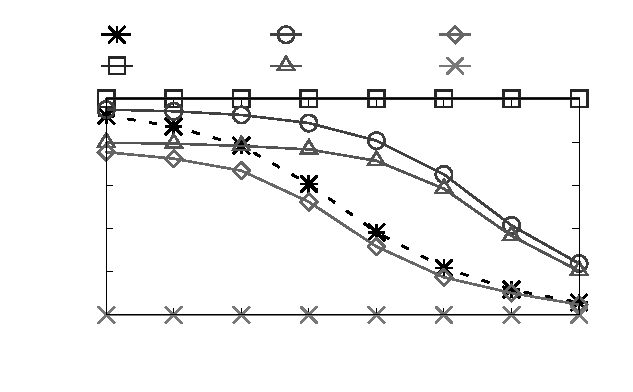
\includegraphics[width={288.00bp},height={172.80bp}]{dummy}}%
    \gplfronttext
  \end{picture}%
\endgroup
}
\caption{Measurement with vs. without declassification\label{fig:jaccardWithDeclass:dummy}}
\end{center}
\end{subfigure}% 
\caption{Declassification example}
\end{figure}

To illustrate the use of
\JaccardWithDeclass{\secretsSetSize}, consider the
simple procedure shown in \figref{code:dummy:proc}.  In this
procedure, $\SecFn{}(\SecVar)$ is an 8-bit value, and \proc simply
outputs the lowest 4 bits as $\AOOFn{}(\AOOVar)$.  The
declassification policy shown in \figref{code:dummy:declass} allows
the \declassifyLo-th to \declassifyHi-th bits of
$\SecFn{}(\SecVar)$ to be released.  We evaluate
\JaccardWithDeclass{\secretsSetSize} with differently
parameterized declassification policies in
\figref{fig:jaccardWithDeclass:dummy}.  Specifically, when the lowest
4 bits ($\declassifyLo=0$, $\declassifyHi=3$) are declassified, then
the additional leakage from \proc is nothing, which is demonstrated by
the ``$\proc+\declassify{0-3}$'' curve. When the declassification
policy declassifies all but the lowest 4 bits ($\declassifyLo=4$,
$\declassifyHi=7$), then the additional leakage by \proc is maximized,
as shown by the ``$\proc+\declassify{4-7}$'' curve.  Intuitively, if
$\AOOFn{}(\AOOVar)$ and $\DCFn{}(\declassifyVar)$ do not overlap
(e.g., ``$\proc+\declassify{4-7}$'' and ``$\proc+\declassify{4-5}$''),
then the \JaccardWithDeclass{\secretsSetSize} curve
should be higher than \JaccardRand{\secretsSetSize}, whereas if
$\AOOFn{}(\AOOVar)$ includes all of $\DCFn{}(\declassifyVar)$ (e.g.,
``$\proc+\declassify{0-3}$'' and ``$\proc+\declassify{0-1}$''), then
\JaccardWithDeclass{\secretsSetSize} should be lower
than \JaccardRand{\secretsSetSize}.  A hybrid case occurs when
$\AOOFn{}(\AOOVar)$ includes a portion of $\DCFn{}(\declassifyVar)$
(e.g., ``$\proc+\declassify{2-5}$''), where
\JaccardWithDeclass{\secretsSetSize} is lower than
\JaccardRand{\secretsSetSize} when \secretsSetSize is small but
becomes larger when \secretsSetSize is large. This is consistent with
the interpretation that \JaccardWithDeclass{\secretsSetSize} with
small \secretsSetSize primarily reflects the number of secret values
for which interference occurs~\cite{sscf}; e.g., when
$\secretsSetSize = 1$, two secret values share bits 0--1 (and so
cannot be distinguished by bits 0--3 after declassifying bits 2--5) in
25\% of cases, but share bits 0--3 (and so cannot be distinguished
using them) in only 6.25\% of cases. Larger \secretsSetSize, in
contrast, better reflects the amount of leakage that
occurs~\cite{sscf}. For example, in a random partition of all $2^8$
values into sets \secretsSet{} and \secretsSetAlt{} of equal size
(i.e., $\secretsSetSize = 2^7$), every value for bits 2--5 is
represented in both \secretsSet{} and \secretsSetAlt{} with high
probability.  In conjunction with the additional bits 0--1 output in
\AOOFn{} (yielding six bits of the secret value in total), however,
these bits give the attacker greater distinguishing power than do bits
0--3 alone.

\section{Interpreting Leakage}
\label{dinome:sec:interpret}

Our defined quantitative leakage metric can measure the interference
of a secret with the outputs observable to the attacker.  For this to
be useful to an analyst, however, it is helpful to provide guidance as
to \textit{why} this leakage occurs.  Specifically, while the
conditions under which leakage occurs are already represented in the
postcondition, it may be difficult to understand the formula without
further help. In this section, we provide a method for generating
short and understandable rules to explain the leakage to a user. 

\subsection{Noninterference and interference tuples}
\label{dinome:sec:interpret:samples}
Our first step toward providing an intuitive explanation 
for the leakage that occurs is to train a binary classifier to
classify 4-tuples
$\langle\ACIFn{},\AIIFn{},\SecFn{},\SecFnAlt{}\rangle$ into those that
illustrate leakage occurring (i.e., that permit the attacker to
distinguish $\SecFn{}(\SecVar)$ and $\SecFnAlt{}(\SecVar)$ from
the resulting output \AOOFn{}) and those that do not.  When using
declassification, the interference tuples should only include those
where the secrets can be distinguished using
$\ACIFn{},\AOOFn{},\DCFn{}$ but not using just $\ACIFn{},\DCFn{}$.

More specifically, we define the interference set \interferenceSet
based on \eqref{eqn:jaccardDeclass:diff}. That is, when the attacker
chooses \ACIFn{}, if an observable value is feasible for $\langle
\AIIFn{}, \SecFn{}\rangle$ for some \AIIFn{} but is never possible for
$\langle \AIIFnAlt{}, \SecFnAlt{}\rangle$ for any \AIIFnAlt{} that
shares a declassification value with $\langle \AIIFn{},
\SecFn{}\rangle$, then $\langle\ACIFn{}, \AIIFn{}, \SecFn{},
\SecFnAlt{}\rangle$ is added to \interferenceSet:
\begin{align}
\interferenceSet 
= \left\{\langle\ACIFn{},\AIIFn{},\SecFn{},\SecFnAlt{}\rangle
\left| \begin{array}[m]{@{\hspace{0.2em}}r@{\hspace{0.25em}}r@{}} 
  \exists \AOOFn{},\DCFn{}
  &:~\hfill \langle \ACIFn{},\AOOFn{},\DCFn{},\AIIFn{}\rangle \in \possibleTriplesWithDeclass{\secretsSet{}}\\
  &\wedge~\hfill
  \langle \ACIFn{},\DCFn{}\rangle \in \possibleDeclass{\secretsSetAlt{}}\cap\possibleDeclass{\secretsSetAlt{}}\\
  &\wedge~\hfill
  \langle \ACIFn{},\AOOFn{},\DCFn{}\rangle \in \possibleDoubleWithDeclass{\secretsSet{}}\setminus\possibleDoubleWithDeclass{\secretsSetAlt{}}
\end{array} 
\right.\right\}
\label{eqn:interferenceSet}
\end{align}
where $\secretsSet{} = \{\SecFn{}(\SecVar)\}$ and $\secretsSetAlt{}
= \{\SecFnAlt{}(\SecVar)\}$.
 
The noninterference set \noninterferenceSet should include two types
of tuples. For an attacker-chosen \ACIFn{}, if there is a observable
value \AOOFn{} that is feasible for an $\langle \AIIFn{},
\SecFn{}\rangle$ pair and an $\langle \AIIFnAlt{}, \SecFnAlt{}\rangle$
pair, tuple $\langle\ACIFn{}, \AIIFn{}, \SecFn{}, \SecFnAlt{}\rangle$
belongs to \noninterferenceSet as it is an example where no
interference occurs.  In addition, for an attacker-chosen \ACIFn{},
if there is a declassification value \DCFn{} that is feasible for
$\langle \AIIFn{}, \SecFn{}\rangle$ but not $\langle\AIIFnAlt{},
\SecFnAlt{}\rangle$ for any \AIIFnAlt{}, then $\langle\ACIFn{},
\AIIFn{}, \SecFn{}, \SecFnAlt{}\rangle$ should also be added to
\noninterferenceSet, as \SecFn{} and \SecFnAlt{} can already be
distinguished using the declassified value:
\begin{align}
\begin{array}{@{}r@{\hspace{0.5em}}r@{}}
\noninterferenceSet =
&\left\{\langle\ACIFn{},\AIIFn{},\SecFn{},\SecFnAlt{}\rangle
\left| \begin{array}[m]{@{\hspace{0.2em}}r@{\hspace{0.25em}}r@{}} 
  \exists \AOOFn, \DCFn{}
  &:~\hfill \langle\ACIFn{}, \AOOFn{}, \DCFn{}, \AIIFn{}\rangle \in \possibleTriplesWithDeclass{\secretsSet{}}
   \wedge~\hfill
  \langle \ACIFn{},\AOOFn{},\DCFn{}\rangle \in \possibleDoubleWithDeclass{\secretsSet{}}\cap\possibleDoubleWithDeclass{\secretsSetAlt{}}
\end{array} 
\right.\right\}\\
& \cup \left\{\langle\ACIFn{},\AIIFn{},\SecFn{},\SecFnAlt{}\rangle
\left| \begin{array}[m]{@{\hspace{0.2em}}r@{\hspace{0.25em}}r@{}} 
  \exists \AOOFn,\DCFn{}
  &:~\hfill \langle \ACIFn{},\AOOFn{},\DCFn{},\AIIFn{}\rangle \in \possibleTriplesWithDeclass{\secretsSet{}}
  \wedge~\hfill
  \langle \ACIFn{},\DCFn{}\rangle \in \possibleDeclass{\secretsSet{}}\setminus \possibleDeclass{\secretsSetAlt{}}
\end{array} 
\right.\right\}
\end{array}
\label{eqn:noninterferenceSet}
\end{align}
where $\secretsSet{} = \{\SecFn{}(\SecVar)\}$ and $\secretsSetAlt{}
= \{\SecFnAlt{}(\SecVar)\}$.

Since \noninterferenceSet and \interferenceSet are large in
practical scenarios, enumerating all tuples is generally
unfeasible.  Instead, we generate samples in each set to train a
machine learning model, from which explanations of the leakage will be
extracted (as described below).  Doing so with modern \sat solvers,
however, typically results in samples that cover \noninterferenceSet
and \interferenceSet unevenly, since solvers generally enumerate
the next solution by simply adding a conflict constraint to block out
previous solutions; as a result, the next solution found is typically
close to the previous.  Another drawback of using this ``blocking''
method to sample is that we cannot parallelize the sampling.

For this reason, we sample from \noninterferenceSet and
\interferenceSet using hash-based sampling
(cf.,~\chapref{chap:sscf}). Specifically, we sample a limited number of
solutions by adding a random universal hashing constraint to the
formula given to the solver. Due to the hash function's universality,
we can run multiple samplers in parallel to generate a large number of
uniformly distributed solutions. In most cases, the sizes of the
sampled sets \noninterferenceSetSamples and \interferenceSetSamples
differ either due to differences in the sizes of \noninterferenceSet
and \interferenceSet or due to the solving difficulty of one set
compared to the other.  We associate a sample weight to each element
to ensure that the weight of each set is equal in the training process
described below.

\subsection{Interpretation through a rule-based method}
\label{dinome:sec:interpret:rules}

Given \noninterferenceSetSamples and \interferenceSetSamples---i.e.,
$\langle\ACIFn{},\AIIFn{},\SecFn{},\SecFnAlt{}\rangle$ tuples labeled
according to whether they illustrate noninterference or
interference---we could train an interpretable machine-learning model
and then extract rules to explain to the user what gives rise to
interference.  A natural such model to consider is a decision tree.
In a decision tree, each decision node (i.e., interior node) is a
predicate on features of a
$\langle\ACIFn{},\AIIFn{},\SecFn{},\SecFnAlt{}\rangle$ tuple, and its
two children correspond to a \boolTrue or \boolFalse evaluation of
this predicate on a tuple, respectively.  A $\langle\ACIFn{}$,
\AIIFn{}, \SecFn{}, $\SecFnAlt{}\rangle$ tuple is classified by
traversing the tree from its root, following the branch from each
decision node corresponding to the result of evaluating the predicate
at that node on the tuple.  Each leaf is labeled with an estimate of
the probability that a tuple constrained by the predicates'
evaluations from the root to that leaf is in \interferenceSet.  We
will discuss what features we include in the process of building
decision trees in \secref{dinome:sec:interpret:features}, but an example
might be individual variables (e.g., $\ACIFn{}(\ACIVar)$).

A single decision tree can easily grow to be deep and complex, and it
can miss some useful combinations of predicates since each decision
predicate is highly influenced by the splits above it in the tree.  To
make the decision tree model more powerful in finding useful
predicates, we used a decision-tree ensemble called gradient boosted
trees~\cite{friedman2001greedy}.  This process produces \gbTreeNmbr
trees denoted $\gbTree{1}, \ldots, \gbTree{\gbTreeNmbr}$, with
associated weights.  If we denote by
$\gbTree{\gbTreeIdx}(\langle\ACIFn{}$, \AIIFn{}, \SecFn{},
$\SecFnAlt{}\rangle)$ the real number stored at the leaf to which
$\langle\ACIFn{}$, \AIIFn{}, \SecFn{}, $\SecFnAlt{}\rangle$ is
assigned by \gbTree{\gbTreeIdx}, then the weighted sum of
$\gbTree{\gbTreeIdx}(\langle\ACIFn{}$ , \AIIFn{}, \SecFn{},
$\SecFnAlt{}\rangle)$ for $\gbTreeIdx = 1, \ldots, \gbTreeNmbr$ is an
estimate of the probability that
$\langle\ACIFn{},\AIIFn{},\SecFn{},\SecFnAlt{}\rangle \in
\interferenceSet$.

To interpret tree ensembles, rule-based classifiers (e.g.,
RuleFit~\cite{friedman2008predictive}, Slipper~\cite{cohen1999simple},
Pre~\cite{fokkema2017pre}) were introduced to bridge the
interpretability of a decision tree with the modeling power of a tree
ensemble.  Our toolchain leverages
\SkopeRule\footnote{\url{https://skope-rules.readthedocs.io/}} to
generate logical rules from the tree ensemble.  Specifically,
consider any path from the root to a leaf in a tree
\gbTree{\gbTreeIdx}, and let $\gbPred{\gbTreeIdx}{1}, \ldots,
\gbPred{\gbTreeIdx}{\gbTreeLevel}$ denote the predicates along that
path that evaluated to \boolTrue.  So, for example, if the first
predicate encountered in \gbTree{\gbTreeIdx}, say ``$\ACIFn{}(\ACIVar)
= 1$'', evaluated to \boolFalse, then \gbPred{\gbTreeIdx}{1} $=$
``$\ACIFn{}(\ACIVar) \neq 1$''.  Then, \SkopeRule constructs a rule by
conjoining $\gbPred{\gbTreeIdx}{1}, \ldots,
\gbPred{\gbTreeIdx}{\gbTreeLevel}$, with the caveat that it limits the
number of predicates included in any rule by heuristically pruning
them.

Each such rule has an associated \textit{precision} and
\textit{recall}, which we evaluate empirically using a validation set
held out from \noninterferenceSetSamples and \interferenceSetSamples
during training.  That is, the \textit{recall} of a rule is the
fraction of validation samples held out from \interferenceSetSamples
for which the rule evaluates to \boolTrue, and the \textit{precision}
of the rule is the fraction of validation samples (from
\interferenceSetSamples or \noninterferenceSetSamples) for which the
rule evaluates to \boolTrue that were held out from
\interferenceSetSamples.  We further prune rules by iteratively
removing conjuncts from a long rule if the precision of the resulting
rule is at least 95\% of the original.  We then rank order rules
according first to precision, and then according to recall.

As we will show, these rules can assist in a quantitative analysis of
the leakage.  For example, a procedure may include a backdoor that
leaks the secret through a specific attacker-controllable condition
(e.g., leaking the secret only when a 64-bit attacker-controlled
variable equals 0). The worst-case interference could be masked by a
large number of weak interferences, as we mentioned in
\secref{sscf:sec:measurement}.  In that case, the interpretable rule
could reveal this specific condition and help the developer
re-evaluate the interference under that condition. The case studies in
\secrefs{dinome:sec:exp:cache}{dinome:sec:exp:modexp} illustrate how
we choose the attacker-controlled inputs based on the interpretable
leakage rules and then re-evaluate the interference caused by a
specific side-channel vector.


\subsection{Feature engineering}
\label{dinome:sec:interpret:features}

The utility of the rule generation described in the previous section
depends critically on the features of each $\langle\ACIFn{}$,
\AIIFn{}, \SecFn{}, $\SecFnAlt{}\rangle$ tuple exposed when training
the tree ensemble, from which the predicates making up the decision
nodes of each tree are formed.  One factor that makes feature
engineering especially critical here is that the \sat solver used to
produce elements of \interferenceSetSamples and
\noninterferenceSetSamples requires that the conditions defining
\interferenceSet and \noninterferenceSet (i.e., conditions
\eqnref{eqn:interferenceSet} and \eqnref{eqn:noninterferenceSet})
be presented to the \sat solver in terms of binary variables only.  As
such, each solution generated by the \sat solver is expressed as an
assignment to these binary variables.  While for some hardware logic,
a binary representation of the relevant variables is most natural, for
other types of logic (e.g., on integers), it is not.

For this reason, we augment each binary solution returned by the \sat
solver (i.e., each $\langle\ACIFn{}$, \AIIFn{}, \SecFn{},
$\SecFnAlt{}\rangle$ tuple) with additional features.  First, we
reconstruct features in a type-aware way from their binary
representations.  For example, if a variable was initially an integer
before being reduced to a collection of binary variables in the
formula presented to the \sat solver, we recover the integer value
from the bit-vector solution and include it as a feature on which the
tree ensemble can trained.  With such type-aware features, predicates
such as, e.g., ``$\SecFn{}(\SecVar)<15$'' can be learned in a
search for simple predicates testing only a single feature, i.e.,
unary predicates.

Unary predicates, however, will be unable to naturally capture some
relationships resulting in leakage.  For example, if leakage happens
only when $\SecFn{}(\SecVar)> \ACIFn{}(\ACIVar)$, permitting
only unary predicates will result in a boundary characterized
point-by-point, e.g., ``$\SecFn{}(\SecVar) \geq \genericThreshold
\wedge \ACIFn{}(\ACIVar)< \genericThreshold$'' where
$\genericThreshold = 1, 2, \ldots$ We thus expanded our feature set
to permit linear combinations of some features (e.g.,
``$\SecFn{}(\SecVar) - \ACIFn{}(\ACIVar)$''), chosen by a
linear classifier described below.  To accommodate branching in the
procedure that results in discontinuities in the boundary between
\interferenceSet and \noninterferenceSet, we opted for a
\textit{local} linear classifier (e.g.,~\cite{fan1993local,
ribeiro2018anchors}).

More specifically, to train the classifier with local constraints, we
pick \textit{anchor points}, around each of which we train a local
classifier that best separates the \textit{nearby} samples in
\interferenceSetSamples and \noninterferenceSetSamples.  (See
\figref{fig:linearfeature}.)  To select anchor points, we first find
pairs of $\langle\ACIFn{}$, \AIIFn{}, \SecFn{}, $\SecFnAlt{}\rangle$
tuples, one from \interferenceSetSamples and one from
\noninterferenceSetSamples, that are \textit{neighbors} in one feature
(i.e., after ranking all tuples by this feature, the pair are adjacent
in the ranking) and then take the pair's \textit{midpoint} tuple as
their per-feature means.  We then select anchors uniformly at random
from these midpoints.  For each anchor, we train a linear classifer
using the tuples in \interferenceSetSamples and
\noninterferenceSetSamples that are within a threshold Euclidean
distance from the anchor.  The linear combination of features used in
this linear classifier is then added as another feature to each
$\langle\ACIFn{}$, \AIIFn{}, \SecFn{}, $\SecFnAlt{}\rangle$ tuple.

\begin{figure}
\centering
\resizebox{0.7\linewidth}{!}
{\protect\small{\input{fig/dinome/localLinearfeature.tex}}}
\caption{Finding linear combinations of features near anchor points
\label{fig:linearfeature}}
\vspace{-4ex}
\end{figure}

\section{Implementation}
\label{dinome:sec:impl}

We developed our approach for evaluating and interpreting leakage,
described in \secref{dinome:sec:measure:declass} and \secref{dinome:sec:interpret}, with an eye toward
applying it to evaluate and understand leakage from hardware designs.
To do so, we define the procedure \proc to be a hardware design, say
written in Verilog, in its initial state but with a predefined program
stored in its memory.  Our system, \thirdsysname, enables the user to
annotate the configuration by marking components of the hardware state
as attacker-controlled (i.e., in \ACIKeys), attacker-observable (in
\AOOKeys), secret (in \SecKeys), or otherwise unknown to the attacker
(in \AIIKeys); to simplify discussion below, we will assume there is
one of each, denoted \ACIVar, \AOOVar, \SecVar, and \AIIVar,
respectively.  Our system converts this ``procedure,'' which we
continue to denote \proc, to a cycle-accurate logical formula
\postcondition{\proc}{} that characterizes hardware execution of the
program and that relates \ACIFn{}, \AOOFn{}, \AIIFn{}, and \SecFn{}.
The user can also declare a declassification function \declassify{}
that operates on the hardware state of the system (we will give
examples below), from which \thirdsysname similarly produces a logical
formula \postcondition{\declassify{}}{} that characterizes how the
declassified information \DCFn{} relates to inputs \ACIFn{}, \AIIFn{},
and \SecFn{} in the execution of \proc. From \postcondition{\proc}{}
and \postcondition{\declassify{}}{}, \thirdsysname generates
\JaccardWithDeclass{\secretsSetSize} for varying \secretsSetSize (see
\eqnref{eqn:jaccardDeclass}) and, if requested, sample sets
\interferenceSetSamples and \noninterferenceSetSamples from
\interferenceSet (see~\eqnref{eqn:interferenceSet}) and
\noninterferenceSet(see~\eqnref{eqn:noninterferenceSet}), respectively.
These sets seed the generation of the rules for interpreting leakage,
as discussed in \secref{dinome:sec:interpret}.

In the subsections below, we will discuss particular challenges we
encountered when building \thirdsysname and how we overcame them. We
focus on how to extract $\postcondition{\proc}{}(\ACIFn{},
\AIIFn{}, \SecFn{}, \AOOFn{})$ in \secref{dinome:sec:impl:logic}.  In
\secref{dinome:sec:impl:preprocess}, we describe simplification techniques we
leverage as a preprocessing step before performing projected model
counting, described in \secref{dinome:sec:impl:counter}.  Finally, we discuss
our technique for sampling to create \interferenceSetSamples and
\noninterferenceSetSamples in \secref{dinome:sec:impl:sampler}.


\subsection{Extracting $\postcondition{\proc}{}(\ACIFn{}, \AIIFn{},
\SecFn{}, \AOOFn{})$} 
\label{dinome:sec:impl:logic}

To analyze the leakage from \proc, we need an accurate postcondition
$\postcondition{\proc}{}(\ACIFn{}, \AIIFn{}, \SecFn{}, \AOOFn{})$ for
\proc. In practice, generating a postcondition for an arbitrary
procedure is not trivial.  Especially here, where our concern is
detecting leakage from a processor implementation when running an
application---i.e., the procedure \proc includes numerous cycles of a
cycle-accurate implementation of the processor logic as well as the
software logic---the postcondition will be quite large.

Our general strategy to construct $\postcondition{\proc}{}(\ACIFn{},
\AIIFn{}, \SecFn{}, \AOOFn{})$ in these circumstances is to assemble
it one cycle at a time. \yosys~\cite{Yosys} provides a framework to
convert the Verilog code for a processor design to its internal
register-transfer level (RTL) intermediate language, optimize or
modify the design using a series of passes, and finally translate the
design to targeted formula through its back-end pass.  The SMT2
back-end pass defines a data structure for each hardware module
representing the module's temporary hardware state, a function to
implement the module's state transition from one cycle to the
next, and an initialization function to initialize the module's state.
To incorporate the software logic of \proc, we compile the software to
its hardware-readable assembly and load the assembly into the
instruction memory unit.

To mark the symbolic variables, the analyst defines a configuration
file to mark as symbolic each input parameter of \proc (in this case,
\SecVar, \AIIVar, and \ACIVar), which can be a software variable
located at a fixed location in the memory unit or a wire/register
inside the hardware module. Our modified \yosys SMT2 backend pass then
tracks the constraints associated with this symbolic data throughout a
cycle execution.  Specifically, it outputs a logical postcondition
$\TmpTransConstraints{\proc}(\HwFn{}{\cycle-1}, \HwFn{}{\cycle})$ that
relates the hardware state $\HwFn{}{\cycle-1} : \HwKeys \rightarrow
\HwVals$ at the end of cycle $\cycle-1$ to the hardware state
\HwFn{}{\cycle} that results from executing cycle \cycle.  We also use
it to generate initialization logic
$\HwPostcondition{\proc}{0}(\ACIFn{}, \AIIFn{}, \SecFn{}, \HwFn{}{0})$
that characterizes the first-cycle starting state \HwFn{}{0} using the
configured symbolic inputs.

Using the transition logic, we construct a cycle-accurate
postcondition \HwPostcondition{\proc}{\ncycles} representing the logic
between symbolic inputs and its internal hardware state one cycle at a
time, leveraging the entire hardware state as an ``observable'' output
of the cycle.
\[\HwPostcondition{\proc}{\ncycles}(\ACIFn{}, \AIIFn{}, \SecFn{}, \HwFn{}{\ncycles})
    \leftarrow 
\HwPostcondition{\proc}{0}(\ACIFn{}, \AIIFn{}, \SecFn{},
\HwFn{}{0}) \wedge
   \bigwedge_{\cycle = 1}^{\ncycles} 
   \TmpTransConstraints{\proc}(\HwFn{}{\cycle-1},\HwFn{}{\cycle})
\]
We finally define $\postcondition{\proc}{}(\ACIFn{},
\AIIFn{}, \SecFn{}, \AOOFn{})$ by defining \AOOFn{} in terms of the sequence of
hardware states $\langle
\HwFn{}{\cycle}\rangle_{\cycle=0}^{\ncycles}$ using a formula
$\glueConstraints{}{}(\langle
\HwFn{}{\cycle}\rangle_{\cycle=0}^{\ncycles}, \AOOFn{})$.
\begin{align}
\postcondition{\proc}{}(\ACIFn{}, \AIIFn{}, \SecFn{}, \AOOFn{})\leftarrow
&\HwPostcondition{\proc}{\ncycles}(\ACIFn{} ,\AIIFn{},\SecFn{},\HwFn{}{\ncycles}) \wedge
\glueConstraints{}{}(\langle\HwFn{}{\cycle}\rangle_{\cycle=0}^{\ncycles}, \AOOFn{})
\label{eqn:build-postcondition}
\end{align}
For example, in cache-based side channels, the observable parameters
are whether there is a cache hit/miss during the execution, which is
constructed using the values of the $s2\_hit$ register across the
execution (as demonstrated in \secref{dinome:sec:exp:cache}).

In our experiments, we selected \ncycles to ensure the termination of
the execution, based on our knowledge gained by studying the CPU.  A
more conservative method would be to track the CPU pipeline and call
the \sat solver each cycle to check whether the last instruction has
certainly committed.  We have confirmed that adding more cycles after
the termination of the execution does not affect
\postcondition{\proc}{} meaningfully, as the additional cycles do not
process any valid opcodes and so only trivially change the hardware
state.

\subsection{Preprocessing formula for \#$\exists$\texttt{SAT}}
\label{dinome:sec:impl:preprocess}
Applying a correct combination of simplification techniques is
critical to scaling the sampling of \interferenceSet and
\noninterferenceSet to create \interferenceSetSamples and
\noninterferenceSetSamples and to count
$\setSize{\possibleTriplesDiffWithDeclass{\secretsSet{}}{\secretsSetAlt{}}}$
and
$\setSize{\possibleTriplesUnionWithDeclass{\secretsSet{}}{\secretsSetAlt{}}}$
to compute \JaccardWithDeclass{\secretsSetSize}.  Langniez et
al.~\cite{lagniez2017preprocessing} provides a summary of the options.
As defined in \secref{dinome:sec:measure:declass} and
\secref{dinome:sec:interpret:samples}, our computation task is
\textit{projected model counting} (\sharpESAT)~\cite{projectedmodelcount} which
counts feasible assignments of selected variables in a propositional
formula. The complexity of the counting problem is \#NP-hard.

To simplify the logical formula, we use preprocessing (similar to that
used in, e.g.,~\cite{klebanov2013sat,manthey2012coprocessor}) that
fully applies equivalence-preserving simplification techniques (e.g.,
vivification and occurrence reduction), and then partially applies
\sat-preserving simplifications (e.g., literal eliminations, variable
eliminations and clause eliminations) targeting variables not in our
counting target (i.e., not marked as \SecVar, \AIIVar, \ACIVar, or
\AOOVar). For example, the partially applied blocked-clause
elimination will remove a clause if it contains a variable not in the
counting target such that every resolvent obtained by resolving on it
is a tautology.  Especially for hardware designs where the number of
possible states increases with the cycle count but many registers are
not modified in some cycles, preprocessing the formula can
substantially reduce the redundancy between the initial and final cycle
formulas.

Although we only need the logic
$\postcondition{\proc}{}(\ACIFn{}, \AIIFn{}, \SecFn{}, \AOOFn{})$ to
describe the relationship between the attacker-observable outputs
\AOOFn{} and inputs \ACIFn{}, \AIIFn{}, \SecFn{} the translated
conjunctive-normal-form (CNF) propositional formula \satProp produced
by the commonly used Tseitin algorithm would have numerous auxiliary
variables.  The number of auxiliary variables and clauses increases
quickly with the number of cycles.  To reduce the use of auxiliary
variables, we applied a state-of-art preprocessing technique for
\textit{model counting} called \BE proposed by Lagniez et
al.~\cite{lagniez2016improving}, who also discussed a possible
application of this method to \textit{projected model counting}.  In
our modified version of \BE, we partition the variables in the CNF
formula representing \postcondition{\proc}{} into two disjoint variable
sets: \supportVars containing the variables in \AIIKeys, \ACIKeys,
\SecKeys, and \AOOKeys, and \reducibleVars containing all other
variables.  For each variable \redVar in \reducibleVars and pair of
clauses $\bar\redVar \vee \negCls{\negIdx}$ and $\redVar \vee
\posCls{\posIdx}$, we then resolve on \redVar and replace the clauses
with their resolvent $\negCls{\negIdx} \vee \posCls{\posIdx}$.  We do
this \textit{only} for variables $\redVar \in \reducibleVars$, since
this ensures:
\begin{align*}
  \left\{\langle \ACIFn{}, \AIIFn{}, \SecFn{}, \AOOFn{}\rangle
  \left|\bigwedge_{\posIdx=0}^{\nposCls}(\redVar \vee \posCls{\posIdx}) \wedge
\bigwedge_{\negIdx=0}^{\nnegCls}(\bar\redVar \vee
\negCls{\negIdx}) \right.\right\}
= \left\{\langle \ACIFn{}, \AIIFn{}, \SecFn{}, \AOOFn{}\rangle
\left| \bigwedge_{\posIdx=0}^{\nposCls}\bigwedge_{\negIdx=0}^{\nnegCls}
(\posCls{\posIdx}\vee\negCls{\negIdx})
\right.\right\}
\end{align*}

Using this algorithm, we eliminate variables in \reducibleVars so that
the final formula uses only \SecVar, \AIIVar, \ACIVar, and \AOOVar
without any auxiliary variables.  This does have the side effect of
introducing more complicated clauses, however, and so we avoid
eliminating $\redVar \in \reducibleVars$ when \redVar is present in
numerous clauses (e.g., $\nnegCls\cdot\nposCls > 500$).
\newcolumntype{d}{D{.}{.}{3.2}}
\begin{table}
\setlength{\tabcolsep}{0.65em}
\renewcommand{\arraystretch}{1.0}
\centering
\footnotesize{
\begin{tabular}{@{}m{30ex}ddddddd@{}}
\toprule
&\multicolumn{7}{d}{cycles} \\
& \multicolumn{1}{d}{5} &	\multicolumn{1}{d}{10} &
\multicolumn{1}{d}{15} & \multicolumn{1}{d}{20} &
\multicolumn{1}{d}{25} & \multicolumn{1}{d}{30} & \multicolumn{1}{d}{35} \\
\midrule
No simplification & 49.1	&  126.6 & 	177.0&	304.2&	459.0&	667.6&	867.6\\[8pt]
Simplified & 1.10	 &1.54	&1.98&	2.03	& 89.9&	167.3&	389.0\\[6pt]
$\sharpESAT$-preprocess& 1.10	 &1.41	&1.45&	1.65	 &1.71&	1.77	&1.88\\
\bottomrule
\end{tabular}
}
\caption[CNF file size for extracted logic formulas]{CNF file size (\megabytes) for logic formulas extracted from
  the RISC-V BOOM core configured with a small application program,
  starting from an initial state with some symbolic memory blocks and
  cache states (see \secref{dinome:sec:exp:cache}).  The CNF file size for a
  one-cycle execution with completely symbolic initial state is
  40\megabytes.  Only computations that terminated within 10 minutes
  are represented.\label{tb:cnf_size}}
\end{table}

In \tabref{tb:cnf_size}, we present example sizes of CNF formulas
generated using different simplification options, for our case studies
in \secref{dinome:sec:exp}.  The row denoted by ``No simplification"
represents the size of a directly translated CNF formula from the
multi-cycle SMT formula, which linearly increases with the number of
cycles. The ``Simplified'' row is generated by directly applying the
CNF simplifications provided by \cryptominisat to the formula in
``Original'', while the row ``\sharpESAT-preprocess'' is
obtained by incrementally applying the preprocessor described in this
section to each \HwPostcondition{\proc}{\ncycles}(\ACIFn{}
,\AIIFn{},\SecFn{},\HwFn{}{\ncycles}) before using it to build
\HwPostcondition{\proc}{\ncycles+1}(\ACIFn{}
,\AIIFn{},\SecFn{},\HwFn{}{\ncycles+1}).


\subsection{Measurement with declassification using projected model
  counting} 
\label{dinome:sec:impl:counter}
Using \cryptominisat as the basic solver, we
implemented a counter to estimate the numerator and the denominator in
the measurement $\JaccardWithDeclass{}(\secretsSet{},
\secretsSetAlt{})$ in \eqref{eqn:jaccardDeclass}.

\subsubsection{Counting $\JaccardWithDeclass{}(\secretsSet{}, \secretsSetAlt{})$}
To compute the measurement $\JaccardWithDeclass{}(\secretsSet{},
\secretsSetAlt{})$, \thirdsysname needs to count the size of
\possibleTriplesDiffWithDeclass{\secretsSet{}}{\secretsSetAlt{}} and
\possibleTriplesUnionWithDeclass{\secretsSet{}}{\secretsSetAlt{}}.
Directly counting
\possibleTriplesDiffWithDeclass{\secretsSet{}}{\secretsSetAlt{}} is
not easy as the set difference operation will introduce a ``forall"
quantifier.  Fortunately, since
$\setSize{\possibleTriplesDiffWithDeclass{\secretsSet{}}{\secretsSetAlt{}}}=
\setSize{\possibleTriplesUnionWithDeclass{\secretsSet{}}{\secretsSetAlt{}}}-
\setSize{\possibleTriplesIntersectWithDeclass{\secretsSet{}}{\secretsSetAlt{}}}$,
it suffices to count
\possibleTriplesUnionWithDeclass{\secretsSet{}}{\secretsSetAlt{}} and
\possibleTriplesIntersectWithDeclass{\secretsSet{}}{\secretsSetAlt{}}
for each sample pair \secretsSet{}, \secretsSetAlt{}. Intuitively,
counting
\possibleTriplesUnionWithDeclass{\secretsSet{}}{\secretsSetAlt{}}
could be expressed as a projected model counting task over
$\langle\ACIFn{}, \AOOFn{}, \AIIFn{}, \SecFn{}\rangle$ in a
quantifier-free SAT problem with two copies of \postcondition{\proc}{}
shown in \satPropUnion below.  \satPropUnion is translated to a CNF
proposition where it uses \satVars bit variables
%denoted by \countTuple
to represent $\langle\ACIFn{}, \AOOFn{}, \DCFn{}, \AIIFn{}\rangle$ and
others to represent $\langle \SecFn{}, \SecFnAlt{}, \AIIFn{},
\AIIFnAlt{}\rangle$ and
auxiliary variables.
\begin{align}
\begin{array}{@{}rr}
\satPropUnion\leftarrow
&\left(\postcondition{\proc}{}(\ACIFn{}, \AIIFn{}, \SecFn{}, \AOOFn{})
\vee
\postcondition{\proc}{}(\ACIFn{}, \AIIFnAlt{}, \SecFnAlt{}, \AOOFn{}) 
\right)\\[4pt]
&\wedge~\hfill
\postcondition{\declassify{}}{}(\ACIFn{}, \AIIFn{}, \SecFn{}, \DCFn{})
\wedge 
\postcondition{\declassify{}}{}(\ACIFn{}, \AIIFnAlt{}, \SecFnAlt{}, \DCFn{})\\[4pt]
&\wedge~\hfill
\left(\begin{array}{@{}r@{}}
(\SecFn{}(\SecVar)\in \secretsSet{}
\wedge
\SecFnAlt{}(\SecVar)\in\secretsSetAlt{}) \\
\vee~
(\SecFnAlt{}(\SecVar)\in \secretsSet{}
\wedge
\SecFn{}(\SecVar)\in\secretsSetAlt{})
\end{array}\right)
\end{array}
\label{eqn:jaccardDeclass:union:imp} 
\end{align}
Following the \secref{sscf:sec:impl:hash:secretsSetSize}, two random,
disjoint sets \secretsSet{} and \secretsSetAlt{} of expected size
\secretsSetSize are specified with distinct strings
$\hashFnOutputPrefix, \hashFnOutputPrefixAlt \in
\{0,1\}^\hashFnOutputPrefixBits$ where $\secretsSetSize =
\setSize{\secretsDomain}/2^\hashFnOutputPrefixBits$, and specifically
with the constraint that for a fixed hash function, the hash of each
$\secretVal \in \secretsSet{}$ is \hashFnOutputPrefix and the hash of
each $\secretValAlt \in \secretsSetAlt{}$ is \hashFnOutputPrefixAlt.

For
\possibleTriplesIntersectWithDeclass{\secretsSet{}}{\secretsSetAlt{}},
we can define another projected model
counting~\cite{projectedmodelcount} task over $\langle\ACIFn{},
\AOOFn{}, \DCFn{}, \AIIFn{}\rangle$ in a quantifier-free SAT problem
\satPropIntersect shown below.  \satPropIntersect uses the logical
postcondition \postcondition{\proc}{} twice, where the first copy is
for the execution with a secret $\SecFn{}(\SecVar) \in \secretsSet{}$
and the second checks for existence of a secret $\SecFnAlt{}(\SecVar)
\in \secretsSetAlt{}$ leading to a result \AOOFn{} also possible with
\SecFn{}.  \satPropIntersect also checks the existence of some secret
(denoted by $\SecFnAltAlt{}(\SecVar)$) in the secret set
\secretsSetAlt{} leading to the equivalent declassification value
\DCFn{} so that we can ensure the \SecFn{} and \SecFnAlt{} cannot be
distinguished by \DCFn{}.

\begin{align}
\begin{array}{@{}rr}
\satPropIntersect\leftarrow
&\postcondition{\proc,\declassify{}}{}(\ACIFn{},\AIIFn{},\SecFn{},
\AOOFn{}, \DCFn{})
\wedge 
\SecFn{}(\SecVar) \in \secretsSet{} \\[4pt]
&\wedge~\hfill
\postcondition{\proc}{}(\ACIFn{}, \AIIFnAlt{}, \SecFnAlt{}, \AOOFn{}) 
\wedge
\SecFnAlt{}(\SecVar) \in\secretsSetAlt{} \\[4pt]
& \wedge~\hfill
\postcondition{\declassify{}}{}(\ACIFn{}, \AIIFnAltAlt{},
\SecFnAltAlt{}, \DCFn{})
\wedge
\SecFnAltAlt{}(\SecVar)\in\secretsSetAlt{}
\end{array}
\label{eqn:jaccardDeclass:intersect:imp} 
\end{align}

\subsubsection{Optimizations for counting
\possibleTriplesDiffWithDeclass{\secretsSet{}}{\secretsSetAlt{}} and
\possibleTriplesUnionWithDeclass{\secretsSet{}}{\secretsSetAlt{}}}
Enumerating all solutions to \eqref{eqn:jaccardDeclass:union:imp} and
\eqref{eqn:jaccardDeclass:intersect:imp} using a solver is
intractable.  To estimate the number of solutions to each instead, we
used the approximate model counting technique due to Chakraborty et
al.~\cite{Chakraborty:2013:SAM:2961240.2961265}, specifically the
approach taken by Soos and Meel~\cite{SM19}.

That is, by specifying a randomly selected hash function
$\hashPrefixFnForIntersect{\hashFnOutputPrefixBitsForIntersect}:
\{0,1\}^{\satVars} \rightarrow
\{0,1\}^{\hashFnOutputPrefixBitsForIntersect}$ and an output
$\hashFnOutputPrefixForIntersect \in
\{0,1\}^{\hashFnOutputPrefixBits}$ as an additional constraint, we can
estimate
\setSize{\possibleTriplesIntersectWithDeclass{\secretsSet{}}{\secretsSetAlt{}}}
using the average value of multiple estimations of
$\setSize{\IntersectWithDeclassSubset{\secretsSet{}}{\secretsSetAlt{}}{\hashFnOutputPrefixForIntersect}}$
with some error \error and confidence \confidence (i.e.,
$\setSize{\possibleTriplesIntersectWithDeclass{\secretsSet{}}{\secretsSetAlt{}}}
\approx $\setSize{\IntersectWithDeclassSubset{\secretsSet{}}{\secretsSetAlt{}}{\hashFnOutputPrefixForIntersect}}$
\times 2^{\hashFnOutputPrefixBitsForIntersect}$).  Similarly, we
could estimate
\setSize{\possibleTriplesUnionWithDeclass{\secretsSet{}}{\secretsSetAlt{}}}
using
\UnionWithDeclassSubset{\secretsSet{}}{\secretsSetAlt{}}{\hashFnOutputPrefixForUnion}.

\begin{align}
\UnionWithDeclassSubset{\secretsSet{}}{\secretsSetAlt{}}{\hashFnOutputPrefixForIntersect}&= \left\{
\langle \ACIFn{},\AOOFn{},\DCFn{},\AIIFn{}\rangle 
 \left|\begin{array}{r}
\langle \ACIFn{},\AOOFn{},\DCFn{},\AIIFn{}\rangle 
\in \possibleTriplesUnionWithDeclass{\secretsSet{}}{\secretsSetAlt{}}
\wedge~\hfill 
\hashPrefixFnForUnion{\hashFnOutputPrefixBitsForUnion}(\langle \ACIFn{},\AOOFn{},\DCFn{},\AIIFn{}\rangle 
)=\hashFnOutputPrefixForUnion
\end{array}
\right.\right\}\\
\IntersectWithDeclassSubset{\secretsSet{}}{\secretsSetAlt{}}{\hashFnOutputPrefixForIntersect}&= \left\{
\langle \ACIFn{},\AOOFn{},\DCFn{},\AIIFn{}\rangle 
 \left|\begin{array}{r}
\langle \ACIFn{},\AOOFn{},\DCFn{},\AIIFn{}\rangle 
 \in \possibleTriplesIntersectWithDeclass{\secretsSet{}}{\secretsSetAlt{}} 
\wedge~\hfill
 \hashPrefixFnForIntersect{\hashFnOutputPrefixBitsForIntersect}(\langle \ACIFn{},\AOOFn{},\DCFn{},\AIIFn{}\rangle)=\hashFnOutputPrefixForIntersect
 \end{array}
\right.\right\}
\end{align}
This optimization for model counting will limit the number of calls to
the \sat solver by constraining the number of solutions available, and
thus make the counting more scalable for large set size. Thus,
\JaccardWithDeclass{}(\secretsSet{}, \secretsSetAlt{})
is estimated using the average value of
$1-\frac{\setSize{\IntersectWithDeclassSubset{\secretsSet{}}{\secretsSetAlt{}}{\hashFnOutputPrefixForIntersect}}}
{\setSize{\UnionWithDeclassSubset{\secretsSet{}}{\secretsSetAlt{}}{\hashFnOutputPrefixForUnion}}}$ for various \hashFnOutputPrefixForIntersect,
\hashFnOutputPrefixForUnion.

Our primary departure from the implementation by Soos and
Meel~\cite{SM19} lies in utilizing task-specific properties in our
counting tasks to reduce redundant effort in solution searching.
Specifically, since
$\possibleTriplesIntersectWithDeclass{\secretsSet{}}{\secretsSetAlt{}}
\subseteq
\possibleTriplesUnionWithDeclass{\secretsSet{}}{\secretsSetAlt{}}$, we
ensure that
$\possibleTriplesIntersectWithDeclass{\secretsSet{}}{\secretsSetAlt{}}
\cap
\UnionWithDeclassSubset{\secretsSet{}}{\secretsSetAlt{}}{\hashFnOutputPrefixForUnion}
\subseteq
\IntersectWithDeclassSubset{\secretsSet{}}{\secretsSetAlt{}}{\hashFnOutputPrefixForIntersect}$
in our counting by defining
$\hashPrefixFnForIntersect{\hashFnOutputPrefixBitsForIntersect}(\langle
\ACIFn{},\AOOFn{},\DCFn{},\AIIFn{}\rangle)$ to be the
\hashFnOutputPrefixBitsForIntersect-bit prefix of
$\hashPrefixFnForUnion{\hashFnOutputPrefixBitsForUnion}(\langle
\ACIFn{},\AOOFn{},\DCFn{},\AIIFn{}\rangle)$ for
$\hashFnOutputPrefixBitsForIntersect \le
\hashFnOutputPrefixBitsForUnion$.  Then once we have generated
solutions in
\UnionWithDeclassSubset{\secretsSet{}}{\secretsSetAlt{}}{\hashFnOutputPrefixForUnion},
we speed up finding solutions in
\IntersectWithDeclassSubset{\secretsSet{}}{\secretsSetAlt{}}{\hashFnOutputPrefixForIntersect}
for $\hashFnOutputPrefixBitsForIntersect =
\hashFnOutputPrefixBitsForUnion$ (and so
$\hashFnOutputPrefixForIntersect = \hashFnOutputPrefixForUnion$) by
first checking each solution in
\UnionWithDeclassSubset{\secretsSet{}}{\secretsSetAlt{}}{\hashFnOutputPrefixForUnion}
to see if it satisfies \satPropIntersect (i.e., is in
$\possibleTriplesIntersectWithDeclass{\secretsSet{}}{\secretsSetAlt{}}
\cap
\UnionWithDeclassSubset{\secretsSet{}}{\secretsSetAlt{}}{\hashFnOutputPrefixForUnion}$).
Only if insufficient solutions are found with
$\hashFnOutputPrefixBitsForIntersect =
\hashFnOutputPrefixBitsForUnion$ is
\hashFnOutputPrefixBitsForIntersect reduced and the solver used to
generate additional solutions in
\IntersectWithDeclassSubset{\secretsSet{}}{\secretsSetAlt{}}{\hashFnOutputPrefixForIntersect}
for \hashFnOutputPrefixForIntersect a
\hashFnOutputPrefixBitsForIntersect-bit prefix of
\hashFnOutputPrefixForUnion.

In the case studies in \secref{dinome:sec:exp}, we set the error $\error=0.4$
and confidence parameter $\confidence=0.9$ in this method of
estimating the sizes of
\possibleTriplesDiffWithDeclass{\secretsSet{}}{\secretsSetAlt{}} and
\possibleTriplesUnionWithDeclass{\secretsSet{}}{\secretsSetAlt{}},
from which $\JaccardWithDeclass{}(\secretsSet{}, \secretsSetAlt{})$ is
estimated using \eqnref{eqn:jaccardDeclass}. For each set size
\secretsSetSize, we compute \JaccardWithDeclass{\secretsSetSize} using
at least 100 hash functions, i.e., implicit selection of pairs
\secretsSet{}, \secretsSetAlt{} of expected size \secretsSetSize.

\subsection{Sampling \noninterferenceSetSamples and
\interferenceSetSamples for interpretable learning} 
\label{dinome:sec:impl:sampler}
Similar to the counting process, to construct
\noninterferenceSetSamples and \interferenceSetSamples, the sampler
will select hash functions \hashPrefixFn{} randomly from a family and
output values \hashFnOutputPrefix randomly from its range to solve for
tuples $\langle \ACIFn{},\AIIFn{},\SecFn{},\SecFnAlt{} \rangle$ for
which $\hashPrefixFn{}(\langle \ACIFn{},\AIIFn{},\SecFn{},\SecFnAlt{}
\rangle) = \hashFnOutputPrefix$ (and are in \noninterferenceSet or
\interferenceSet, respectively).  In the following experiments, we
will generate up to 100,000 solutions for each of
\noninterferenceSetSamples and \interferenceSetSamples, where 70\%
used for training and 30\% used for validation.

We cannot directly encode set difference, used in
\eqref{eqn:interferenceSet} and \eqref{eqn:noninterferenceSet}, using
an equivalent quantifier-free formula. To implement a sampler to
generate solutions in the set difference, we will use one solver
(``E-solver'') to search for candidate solutions and another
(``F-solver'') cancel candidates; this is a commonly used algorithm
for an SMT solver to solve exist-forall problems (e.g.,
see~\cite{dutertre2015solving}).  Here, we will illustrate sampling
\interferenceSet, while sampling \noninterferenceSet is similar.

\begin{figure}[tb]
\noindent
\interferenceSuperTest with \hashPrefixFn{} and \hashFnOutputPrefix{}
generates
$\langle\ACIFn{},\AIIFn{},\SecFn{},\SecFnAlt{},\AOOFn{},\DCFn{}\rangle$
satisfying
\begin{align}
\begin{array}[m]{rr}
\postcondition{\proc,\declassify{}}{}(\ACIFn{}, \AIIFn{}, \SecFn{},
\AOOFn{}, \DCFn{})
\wedge
\postcondition{\proc,\declassify{}}{}(\ACIFn{}, \AIIFnAlt{},
\SecFnAlt{}, \AOOFnAlt{}, \DCFn{})
\wedge  \AOOFn{} \neq \AOOFnAlt{} \wedge
\hashPrefixFn{}(\ACIFn{},\AIIFn{},\SecFn{},\SecFnAlt{})=\hashFnOutputPrefix
\end{array}
\label{eqn:interferenceSuperTest} 
\end{align}

\noindent
\interferenceFalseTest{} cancels
$\langle\ACIFn{},\AIIFn{},\SecFn{},\SecFnAlt{},\AOOFn{},\DCFn{}\rangle$
satisfying \eqnref{eqn:interferenceSuperTest} if there is some
\AIIFnAltAlt{} satisfying
\begin{align}
\begin{array}[m]{rr}
\postcondition{\proc,\declassify{}}{}(\ACIFn{}, \AIIFnAltAlt{},
\SecFnAlt{}, \AOOFn{}, \DCFn{})
\end{array}
\label{eqn:interferenceFalseTest}
\end{align}
\caption{Generating examples in \interferenceSetSamples using
EF-solver\label{fig:ef-solver}}
\end{figure}

Specifically, the sampler first uses the \interferenceSuperTest to
generate feasible solutions \sampleTuple (see
\eqref{eqn:interferenceSuperTest}) that guarantee, for an attacker's
choosen \ACIFn{}, the observable value \AOOFn{} derived from \SecFn{}
with \AIIFn{} could be different from an observable \AOOFnAlt{}
generated by \SecFnAlt{} with some \AIIFnAlt{}
when the declassified value \DCFn{} is the same.  However, it does not
guarantee the \AOOFn{} is never feasible for \SecFn{}. To further test
whether the \sampleTuple is in \interferenceSetSamples, we use the
\interferenceFalseTest to test whether
$\langle\AIIFnAltAlt{}, \SecFnAlt{}\rangle$ for some \AIIFnAltAlt{}
could generate \AOOFn{} with $\langle\AIIFn{},\SecFn{}\rangle$ when
they share the declassification value \DCFn{}, to check whether we
need to cancel the solution.  That is, \sampleTuple satisfying
\eqref{eqn:interferenceSuperTest} but not
\eqref{eqn:interferenceFalseTest} will be included in
\interferenceSetSamples{}.

After generating enough $\sampleTuple$ tuples in
\noninterferenceSetSamples and \interferenceSetSamples, the
interpretation module trains local support vector machine (SVM)
classifiers \cite{fan2008liblinear} around each of 50 anchor points,
after ruling out data whose normalized Euclidean distance (i.e., after
scaling each attribute to a value between 0 and 1, use Euclidean
distance divided by the number of attributes) is more than $0.2$ from
the anchor.
%\textit{LinearSVC} with \textit{L1} penalty and sample weights which
%are balanced
Then a logistic regression model for \noninterferenceSet and
\interferenceSet is learned using a gradient boosted tree
implementation \textit{xgboost}~\cite{chen2016xgboost}. To generate the
interpretable models, we implemented the rule learner using \SkopeRule.

\section{Case Studies} 
\label{dinome:sec:exp}
In this section, we illustrate \thirdsysname by describing its application
to the \boom core (\url{https://github.com/riscv-boom/riscv-boom}), an
open-source RISC-V core that is susceptible to cache-based side
channels and \spectre attacks.  The goal of these case studies was to
illustrate our methodology and to show how it can be useful to system
analysts.  We require these analysts to specify the secret to protect
and attacker-controlled and attacker-observable variables but,
critically, not the specific attacker algorithm.
\begin{compactitem}
\item We applied \thirdsysname to evaluate cache-based side-channel leakage
  due to secret-dependent memory accesses. With different parameter
  configurations for \boom (i.e., number of cache ways \cacheLineNmbr
  and whether to enable memory sharing), this case study shows how
  \JaccardWithDeclass{\secretsSetSize}{} curves demonstrate the
  effects of these settings on the leakage.  Moreover, we implemented
  and evaluated two possible mitigations, namely
  \scatterCache~\cite{scatterCache} and
  \phantomCache~\cite{phantomCache}, both of which use a
  per-security-domain memory-to-cache mapping to reduce but not
  eliminate the cache leakage.  Our measurements using
  \JaccardWithDeclass{\secretsSetSize}{} illustrate which mitigation
  is better for a specific \boom setting.
\item We used \thirdsysname to demonstrate information leakage due to
  cache-based side channels from a modular exponentiation function
  commonly used in cryptographic algorithms.  The rule-based
  interpretation explains how to choose attacker-controlled variables
  and which portion of the secret are leaked.
\item We evaluated software code snippets causing speculative
  execution and demonstrated how to use declassification to narrow in
  on leakage caused by speculative execution (i.e., by declassifying
other leakage to reveal it).  We found that some software with a short
speculative window is not sufficient to cause out-of-bound memory
leakage in the latest version of \boom.
\end{compactitem}

 
\subsection{\boom configurations}

\begin{figure}
\centering
%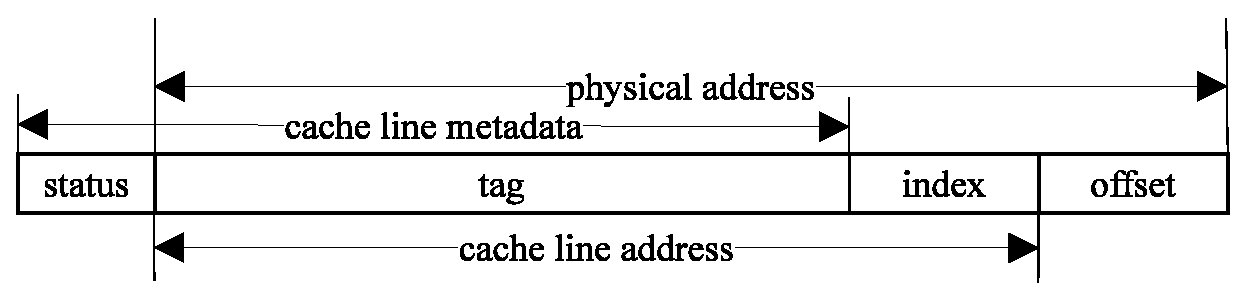
\includegraphics[width=\linewidth]{fig/dinome/tagarray.eps}
\resizebox{0.6\linewidth}{!}{\protect\scriptsize% Graphic for TeX using PGF
% Title: /Users/ziqiaozhou/zzdiss/paper/fig/tagarray_new.dia
% Creator: Dia v0.97.2
% CreationDate: Thu Jun 18 03:05:38 2020
% For: ziqiao
% \usepackage{tikz}
% The following commands are not supported in PSTricks at present
% We define them conditionally, so when they are implemented,
% this pgf file will use them.
\ifx\du\undefined
  \newlength{\du}
\fi
\setlength{\du}{15\unitlength}
\begin{tikzpicture}
\pgftransformxscale{1.000000}
\pgftransformyscale{-1.000000}
\definecolor{dialinecolor}{rgb}{0.000000, 0.000000, 0.000000}
\pgfsetstrokecolor{dialinecolor}
\definecolor{dialinecolor}{rgb}{1.000000, 1.000000, 1.000000}
\pgfsetfillcolor{dialinecolor}
\pgfsetlinewidth{0.100000\du}
\pgfsetdash{{1.000000\du}{1.000000\du}}{0\du}
\pgfsetdash{{0.100000\du}{0.100000\du}}{0\du}
\pgfsetmiterjoin
\definecolor{dialinecolor}{rgb}{1.000000, 1.000000, 1.000000}
\pgfsetfillcolor{dialinecolor}
\fill (27.608400\du,2.495308\du)--(27.608400\du,3.495308\du)--(29.941231\du,3.495308\du)--(29.941231\du,2.495308\du)--cycle;
\definecolor{dialinecolor}{rgb}{0.000000, 0.000000, 0.000000}
\pgfsetstrokecolor{dialinecolor}
\draw (27.608400\du,2.495308\du)--(27.608400\du,3.495308\du)--(29.941231\du,3.495308\du)--(29.941231\du,2.495308\du)--cycle;
\pgfsetlinewidth{0.100000\du}
\pgfsetdash{{0.100000\du}{0.100000\du}}{0\du}
\pgfsetdash{{0.100000\du}{0.100000\du}}{0\du}
\pgfsetmiterjoin
\definecolor{dialinecolor}{rgb}{1.000000, 1.000000, 1.000000}
\pgfsetfillcolor{dialinecolor}
\fill (27.609100\du,3.482218\du)--(27.609100\du,4.482218\du)--(29.941165\du,4.482218\du)--(29.941165\du,3.482218\du)--cycle;
\definecolor{dialinecolor}{rgb}{0.000000, 0.000000, 0.000000}
\pgfsetstrokecolor{dialinecolor}
\draw (27.609100\du,3.482218\du)--(27.609100\du,4.482218\du)--(29.941165\du,4.482218\du)--(29.941165\du,3.482218\du)--cycle;
\pgfsetlinewidth{0.100000\du}
\pgfsetdash{{0.100000\du}{0.100000\du}}{0\du}
\pgfsetdash{{0.100000\du}{0.100000\du}}{0\du}
\pgfsetmiterjoin
\definecolor{dialinecolor}{rgb}{1.000000, 1.000000, 1.000000}
\pgfsetfillcolor{dialinecolor}
\fill (25.970500\du,2.496208\du)--(25.970500\du,3.488975\du)--(27.605876\du,3.488975\du)--(27.605876\du,2.496208\du)--cycle;
\definecolor{dialinecolor}{rgb}{0.000000, 0.000000, 0.000000}
\pgfsetstrokecolor{dialinecolor}
\draw (25.970500\du,2.496208\du)--(25.970500\du,3.488975\du)--(27.605876\du,3.488975\du)--(27.605876\du,2.496208\du)--cycle;
\pgfsetlinewidth{0.100000\du}
\pgfsetdash{{0.100000\du}{0.100000\du}}{0\du}
\pgfsetdash{{0.100000\du}{0.100000\du}}{0\du}
\pgfsetmiterjoin
\definecolor{dialinecolor}{rgb}{1.000000, 1.000000, 1.000000}
\pgfsetfillcolor{dialinecolor}
\fill (24.270900\du,2.496208\du)--(24.270900\du,3.488975\du)--(25.963313\du,3.488975\du)--(25.963313\du,2.496208\du)--cycle;
\definecolor{dialinecolor}{rgb}{0.000000, 0.000000, 0.000000}
\pgfsetstrokecolor{dialinecolor}
\draw (24.270900\du,2.496208\du)--(24.270900\du,3.488975\du)--(25.963313\du,3.488975\du)--(25.963313\du,2.496208\du)--cycle;
\pgfsetlinewidth{0.100000\du}
\pgfsetdash{{0.100000\du}{0.100000\du}}{0\du}
\pgfsetdash{{0.100000\du}{0.100000\du}}{0\du}
\pgfsetmiterjoin
\definecolor{dialinecolor}{rgb}{1.000000, 1.000000, 1.000000}
\pgfsetfillcolor{dialinecolor}
\fill (25.962300\du,3.491218\du)--(25.962300\du,4.483985\du)--(27.597676\du,4.483985\du)--(27.597676\du,3.491218\du)--cycle;
\definecolor{dialinecolor}{rgb}{0.000000, 0.000000, 0.000000}
\pgfsetstrokecolor{dialinecolor}
\draw (25.962300\du,3.491218\du)--(25.962300\du,4.483985\du)--(27.597676\du,4.483985\du)--(27.597676\du,3.491218\du)--cycle;
\pgfsetlinewidth{0.100000\du}
\pgfsetdash{{0.100000\du}{0.100000\du}}{0\du}
\pgfsetdash{{0.100000\du}{0.100000\du}}{0\du}
\pgfsetmiterjoin
\definecolor{dialinecolor}{rgb}{1.000000, 1.000000, 1.000000}
\pgfsetfillcolor{dialinecolor}
\fill (24.262700\du,3.491218\du)--(24.262700\du,4.483985\du)--(25.955113\du,4.483985\du)--(25.955113\du,3.491218\du)--cycle;
\definecolor{dialinecolor}{rgb}{0.000000, 0.000000, 0.000000}
\pgfsetstrokecolor{dialinecolor}
\draw (24.262700\du,3.491218\du)--(24.262700\du,4.483985\du)--(25.955113\du,4.483985\du)--(25.955113\du,3.491218\du)--cycle;
\pgfsetlinewidth{0.030000\du}
\pgfsetdash{}{0pt}
\pgfsetdash{}{0pt}
\pgfsetmiterjoin
\definecolor{dialinecolor}{rgb}{1.000000, 1.000000, 1.000000}
\pgfsetfillcolor{dialinecolor}
\fill (27.929900\du,1.816670\du)--(27.929900\du,2.816670\du)--(30.262731\du,2.816670\du)--(30.262731\du,1.816670\du)--cycle;
\definecolor{dialinecolor}{rgb}{0.000000, 0.000000, 0.000000}
\pgfsetstrokecolor{dialinecolor}
\draw (27.929900\du,1.816670\du)--(27.929900\du,2.816670\du)--(30.262731\du,2.816670\du)--(30.262731\du,1.816670\du)--cycle;
\pgfsetlinewidth{0.030000\du}
\pgfsetdash{}{0pt}
\pgfsetdash{}{0pt}
\pgfsetmiterjoin
\definecolor{dialinecolor}{rgb}{1.000000, 1.000000, 1.000000}
\pgfsetfillcolor{dialinecolor}
\fill (27.930600\du,2.803580\du)--(27.930600\du,3.803580\du)--(30.262665\du,3.803580\du)--(30.262665\du,2.803580\du)--cycle;
\definecolor{dialinecolor}{rgb}{0.000000, 0.000000, 0.000000}
\pgfsetstrokecolor{dialinecolor}
\draw (27.930600\du,2.803580\du)--(27.930600\du,3.803580\du)--(30.262665\du,3.803580\du)--(30.262665\du,2.803580\du)--cycle;
\pgfsetlinewidth{0.030000\du}
\pgfsetdash{}{0pt}
\pgfsetdash{}{0pt}
\pgfsetmiterjoin
\definecolor{dialinecolor}{rgb}{1.000000, 1.000000, 1.000000}
\pgfsetfillcolor{dialinecolor}
\fill (26.292000\du,1.817570\du)--(26.292000\du,2.810338\du)--(27.927376\du,2.810338\du)--(27.927376\du,1.817570\du)--cycle;
\definecolor{dialinecolor}{rgb}{0.000000, 0.000000, 0.000000}
\pgfsetstrokecolor{dialinecolor}
\draw (26.292000\du,1.817570\du)--(26.292000\du,2.810338\du)--(27.927376\du,2.810338\du)--(27.927376\du,1.817570\du)--cycle;
\pgfsetlinewidth{0.030000\du}
\pgfsetdash{}{0pt}
\pgfsetdash{}{0pt}
\pgfsetmiterjoin
\definecolor{dialinecolor}{rgb}{1.000000, 1.000000, 1.000000}
\pgfsetfillcolor{dialinecolor}
\fill (24.592400\du,1.817570\du)--(24.592400\du,2.810338\du)--(26.284813\du,2.810338\du)--(26.284813\du,1.817570\du)--cycle;
\definecolor{dialinecolor}{rgb}{0.000000, 0.000000, 0.000000}
\pgfsetstrokecolor{dialinecolor}
\draw (24.592400\du,1.817570\du)--(24.592400\du,2.810338\du)--(26.284813\du,2.810338\du)--(26.284813\du,1.817570\du)--cycle;
\pgfsetlinewidth{0.030000\du}
\pgfsetdash{}{0pt}
\pgfsetdash{}{0pt}
\pgfsetmiterjoin
\definecolor{dialinecolor}{rgb}{1.000000, 1.000000, 1.000000}
\pgfsetfillcolor{dialinecolor}
\fill (26.283800\du,2.812580\du)--(26.283800\du,3.805348\du)--(27.919176\du,3.805348\du)--(27.919176\du,2.812580\du)--cycle;
\definecolor{dialinecolor}{rgb}{0.000000, 0.000000, 0.000000}
\pgfsetstrokecolor{dialinecolor}
\draw (26.283800\du,2.812580\du)--(26.283800\du,3.805348\du)--(27.919176\du,3.805348\du)--(27.919176\du,2.812580\du)--cycle;
\pgfsetlinewidth{0.030000\du}
\pgfsetdash{}{0pt}
\pgfsetdash{}{0pt}
\pgfsetmiterjoin
\definecolor{dialinecolor}{rgb}{1.000000, 1.000000, 1.000000}
\pgfsetfillcolor{dialinecolor}
\fill (24.584200\du,2.812580\du)--(24.584200\du,3.805348\du)--(26.276613\du,3.805348\du)--(26.276613\du,2.812580\du)--cycle;
\definecolor{dialinecolor}{rgb}{0.000000, 0.000000, 0.000000}
\pgfsetstrokecolor{dialinecolor}
\draw (24.584200\du,2.812580\du)--(24.584200\du,3.805348\du)--(26.276613\du,3.805348\du)--(26.276613\du,2.812580\du)--cycle;
\pgfsetlinewidth{0.030000\du}
\pgfsetdash{}{0pt}
\pgfsetdash{}{0pt}
\pgfsetmiterjoin
\definecolor{dialinecolor}{rgb}{1.000000, 1.000000, 1.000000}
\pgfsetfillcolor{dialinecolor}
\fill (28.344400\du,1.133710\du)--(28.344400\du,2.133710\du)--(30.677231\du,2.133710\du)--(30.677231\du,1.133710\du)--cycle;
\definecolor{dialinecolor}{rgb}{0.000000, 0.000000, 0.000000}
\pgfsetstrokecolor{dialinecolor}
\draw (28.344400\du,1.133710\du)--(28.344400\du,2.133710\du)--(30.677231\du,2.133710\du)--(30.677231\du,1.133710\du)--cycle;
\pgfsetlinewidth{0.030000\du}
\pgfsetdash{}{0pt}
\pgfsetdash{}{0pt}
\pgfsetmiterjoin
\definecolor{dialinecolor}{rgb}{1.000000, 1.000000, 1.000000}
\pgfsetfillcolor{dialinecolor}
\fill (28.345100\du,2.120620\du)--(28.345100\du,3.120620\du)--(30.677165\du,3.120620\du)--(30.677165\du,2.120620\du)--cycle;
\definecolor{dialinecolor}{rgb}{0.000000, 0.000000, 0.000000}
\pgfsetstrokecolor{dialinecolor}
\draw (28.345100\du,2.120620\du)--(28.345100\du,3.120620\du)--(30.677165\du,3.120620\du)--(30.677165\du,2.120620\du)--cycle;
\pgfsetlinewidth{0.030000\du}
\pgfsetdash{}{0pt}
\pgfsetdash{}{0pt}
\pgfsetmiterjoin
\definecolor{dialinecolor}{rgb}{1.000000, 1.000000, 1.000000}
\pgfsetfillcolor{dialinecolor}
\fill (26.706500\du,1.134610\du)--(26.706500\du,2.127378\du)--(28.341876\du,2.127378\du)--(28.341876\du,1.134610\du)--cycle;
\definecolor{dialinecolor}{rgb}{0.000000, 0.000000, 0.000000}
\pgfsetstrokecolor{dialinecolor}
\draw (26.706500\du,1.134610\du)--(26.706500\du,2.127378\du)--(28.341876\du,2.127378\du)--(28.341876\du,1.134610\du)--cycle;
\pgfsetlinewidth{0.030000\du}
\pgfsetdash{}{0pt}
\pgfsetdash{}{0pt}
\pgfsetmiterjoin
\definecolor{dialinecolor}{rgb}{1.000000, 1.000000, 1.000000}
\pgfsetfillcolor{dialinecolor}
\fill (25.006900\du,1.134610\du)--(25.006900\du,2.127378\du)--(26.699313\du,2.127378\du)--(26.699313\du,1.134610\du)--cycle;
\definecolor{dialinecolor}{rgb}{0.000000, 0.000000, 0.000000}
\pgfsetstrokecolor{dialinecolor}
\draw (25.006900\du,1.134610\du)--(25.006900\du,2.127378\du)--(26.699313\du,2.127378\du)--(26.699313\du,1.134610\du)--cycle;
\pgfsetlinewidth{0.030000\du}
\pgfsetdash{}{0pt}
\pgfsetdash{}{0pt}
\pgfsetmiterjoin
\definecolor{dialinecolor}{rgb}{1.000000, 1.000000, 1.000000}
\pgfsetfillcolor{dialinecolor}
\fill (26.698300\du,2.129620\du)--(26.698300\du,3.122388\du)--(28.333676\du,3.122388\du)--(28.333676\du,2.129620\du)--cycle;
\definecolor{dialinecolor}{rgb}{0.000000, 0.000000, 0.000000}
\pgfsetstrokecolor{dialinecolor}
\draw (26.698300\du,2.129620\du)--(26.698300\du,3.122388\du)--(28.333676\du,3.122388\du)--(28.333676\du,2.129620\du)--cycle;
\pgfsetlinewidth{0.030000\du}
\pgfsetdash{}{0pt}
\pgfsetdash{}{0pt}
\pgfsetmiterjoin
\definecolor{dialinecolor}{rgb}{1.000000, 1.000000, 1.000000}
\pgfsetfillcolor{dialinecolor}
\fill (24.998700\du,2.129620\du)--(24.998700\du,3.122388\du)--(26.691113\du,3.122388\du)--(26.691113\du,2.129620\du)--cycle;
\definecolor{dialinecolor}{rgb}{0.000000, 0.000000, 0.000000}
\pgfsetstrokecolor{dialinecolor}
\draw (24.998700\du,2.129620\du)--(24.998700\du,3.122388\du)--(26.691113\du,3.122388\du)--(26.691113\du,2.129620\du)--cycle;
\definecolor{dialinecolor}{rgb}{1.000000, 1.000000, 1.000000}
\pgfsetfillcolor{dialinecolor}
\fill (21.823667\du,1.111950\du)--(23.275433\du,2.126726\du)--(21.823667\du,3.141502\du)--(20.371900\du,2.126726\du)--cycle;
\pgfsetlinewidth{0.050000\du}
\pgfsetdash{}{0pt}
\pgfsetdash{}{0pt}
\pgfsetmiterjoin
\definecolor{dialinecolor}{rgb}{0.000000, 0.000000, 0.000000}
\pgfsetstrokecolor{dialinecolor}
\draw (21.823667\du,1.111950\du)--(23.275433\du,2.126726\du)--(21.823667\du,3.141502\du)--(20.371900\du,2.126726\du)--cycle;
% setfont left to latex
\definecolor{dialinecolor}{rgb}{0.000000, 0.000000, 0.000000}
\pgfsetstrokecolor{dialinecolor}
\node at (21.823667\du,2.296726\du){Match};
\pgfsetlinewidth{0.030000\du}
\pgfsetdash{}{0pt}
\pgfsetdash{}{0pt}
\pgfsetbuttcap
{
\definecolor{dialinecolor}{rgb}{0.000000, 0.000000, 0.000000}
\pgfsetfillcolor{dialinecolor}
% was here!!!
\pgfsetarrowsstart{latex}
\pgfsetarrowsend{latex}
\definecolor{dialinecolor}{rgb}{0.000000, 0.000000, 0.000000}
\pgfsetstrokecolor{dialinecolor}
\draw (17.397100\du,0.551166\du)--(23.224850\du,0.539583\du);
}
\definecolor{dialinecolor}{rgb}{1.000000, 1.000000, 1.000000}
\pgfsetfillcolor{dialinecolor}
\fill (17.979700\du,-0.024626\du)--(17.979700\du,0.682874\du)--(22.642200\du,0.682874\du)--(22.642200\du,-0.024626\du)--cycle;
% setfont left to latex
\definecolor{dialinecolor}{rgb}{0.000000, 0.000000, 0.000000}
\pgfsetstrokecolor{dialinecolor}
\node at (20.310950\du,0.545374\du){cache line address};
\pgfsetlinewidth{0.030000\du}
\pgfsetdash{}{0pt}
\pgfsetdash{}{0pt}
\pgfsetbuttcap
{
\definecolor{dialinecolor}{rgb}{0.000000, 0.000000, 0.000000}
\pgfsetfillcolor{dialinecolor}
% was here!!!
\definecolor{dialinecolor}{rgb}{0.000000, 0.000000, 0.000000}
\pgfsetstrokecolor{dialinecolor}
\draw (17.379900\du,0.073392\du)--(17.380700\du,1.023490\du);
}
\pgfsetlinewidth{0.030000\du}
\pgfsetdash{}{0pt}
\pgfsetdash{}{0pt}
\pgfsetbuttcap
{
\definecolor{dialinecolor}{rgb}{0.000000, 0.000000, 0.000000}
\pgfsetfillcolor{dialinecolor}
% was here!!!
\definecolor{dialinecolor}{rgb}{0.000000, 0.000000, 0.000000}
\pgfsetstrokecolor{dialinecolor}
\draw (23.226000\du,0.074327\du)--(23.223700\du,1.004840\du);
}
\pgfsetlinewidth{0.030000\du}
\pgfsetdash{}{0pt}
\pgfsetdash{}{0pt}
\pgfsetbuttcap
{
\definecolor{dialinecolor}{rgb}{0.000000, 0.000000, 0.000000}
\pgfsetfillcolor{dialinecolor}
% was here!!!
\definecolor{dialinecolor}{rgb}{0.000000, 0.000000, 0.000000}
\pgfsetstrokecolor{dialinecolor}
\draw (25.741900\du,-1.833290\du)--(25.735600\du,-0.925673\du);
}
\pgfsetlinewidth{0.030000\du}
\pgfsetdash{}{0pt}
\pgfsetdash{}{0pt}
\pgfsetbuttcap
{
\definecolor{dialinecolor}{rgb}{0.000000, 0.000000, 0.000000}
\pgfsetfillcolor{dialinecolor}
% was here!!!
\definecolor{dialinecolor}{rgb}{0.000000, 0.000000, 0.000000}
\pgfsetstrokecolor{dialinecolor}
\draw (17.389200\du,-1.830420\du)--(17.379900\du,-0.926608\du);
}
\pgfsetlinewidth{0.030000\du}
\pgfsetdash{}{0pt}
\pgfsetdash{}{0pt}
\pgfsetbuttcap
{
\definecolor{dialinecolor}{rgb}{0.000000, 0.000000, 0.000000}
\pgfsetfillcolor{dialinecolor}
% was here!!!
\pgfsetarrowsstart{latex}
\pgfsetarrowsend{latex}
\definecolor{dialinecolor}{rgb}{0.000000, 0.000000, 0.000000}
\pgfsetstrokecolor{dialinecolor}
\draw (17.384550\du,-1.378514\du)--(25.738750\du,-1.379482\du);
}
\definecolor{dialinecolor}{rgb}{1.000000, 1.000000, 1.000000}
\pgfsetfillcolor{dialinecolor}
\fill (19.434400\du,-1.983580\du)--(19.434400\du,-1.276080\du)--(23.654400\du,-1.276080\du)--(23.654400\du,-1.983580\du)--cycle;
% setfont left to latex
\definecolor{dialinecolor}{rgb}{0.000000, 0.000000, 0.000000}
\pgfsetstrokecolor{dialinecolor}
\node at (21.544400\du,-1.413580\du){physical address};
\pgfsetlinewidth{0.080000\du}
\pgfsetdash{}{0pt}
\pgfsetdash{}{0pt}
\pgfsetmiterjoin
\pgfsetbuttcap
{
\definecolor{dialinecolor}{rgb}{0.000000, 0.000000, 0.000000}
\pgfsetfillcolor{dialinecolor}
% was here!!!
{\pgfsetcornersarced{\pgfpoint{0.000000\du}{0.000000\du}}\definecolor{dialinecolor}{rgb}{0.000000, 0.000000, 0.000000}
\pgfsetstrokecolor{dialinecolor}
\draw (21.823667\du,3.141502\du)--(21.823667\du,3.555504\du)--(23.476300\du,3.555504\du)--(23.476300\du,2.992591\du)--(24.270900\du,2.992591\du);
}}
\pgfsetlinewidth{0.080000\du}
\pgfsetdash{}{0pt}
\pgfsetdash{}{0pt}
\pgfsetmiterjoin
\pgfsetbuttcap
{
\definecolor{dialinecolor}{rgb}{0.000000, 0.000000, 0.000000}
\pgfsetfillcolor{dialinecolor}
% was here!!!
{\pgfsetcornersarced{\pgfpoint{0.000000\du}{0.000000\du}}\definecolor{dialinecolor}{rgb}{0.000000, 0.000000, 0.000000}
\pgfsetstrokecolor{dialinecolor}
\draw (21.823667\du,3.141502\du)--(21.823667\du,4.000119\du)--(23.659100\du,4.000119\du)--(23.659100\du,3.987601\du)--(24.262700\du,3.987601\du);
}}
\pgfsetlinewidth{0.080000\du}
\pgfsetdash{}{0pt}
\pgfsetdash{}{0pt}
\pgfsetbuttcap
{
\definecolor{dialinecolor}{rgb}{0.000000, 0.000000, 0.000000}
\pgfsetfillcolor{dialinecolor}
% was here!!!
\pgfsetarrowsend{stealth}
\definecolor{dialinecolor}{rgb}{0.000000, 0.000000, 0.000000}
\pgfsetstrokecolor{dialinecolor}
\draw (21.816800\du,0.073392\du)--(21.823667\du,1.111950\du);
}
\pgfsetlinewidth{0.050000\du}
\pgfsetdash{}{0pt}
\pgfsetdash{}{0pt}
\pgfsetmiterjoin
\definecolor{dialinecolor}{rgb}{1.000000, 1.000000, 1.000000}
\pgfsetfillcolor{dialinecolor}
\fill (17.379900\du,-0.926608\du)--(17.379900\du,0.073392\du)--(20.402119\du,0.073392\du)--(20.402119\du,-0.926608\du)--cycle;
\definecolor{dialinecolor}{rgb}{0.000000, 0.000000, 0.000000}
\pgfsetstrokecolor{dialinecolor}
\draw (17.379900\du,-0.926608\du)--(17.379900\du,0.073392\du)--(20.402119\du,0.073392\du)--(20.402119\du,-0.926608\du)--cycle;
\pgfsetlinewidth{0.050000\du}
\pgfsetdash{}{0pt}
\pgfsetdash{}{0pt}
\pgfsetmiterjoin
\definecolor{dialinecolor}{rgb}{1.000000, 1.000000, 1.000000}
\pgfsetfillcolor{dialinecolor}
\fill (20.417300\du,-0.926608\du)--(20.417300\du,0.073392\du)--(23.216400\du,0.073392\du)--(23.216400\du,-0.926608\du)--cycle;
\definecolor{dialinecolor}{rgb}{0.000000, 0.000000, 0.000000}
\pgfsetstrokecolor{dialinecolor}
\draw (20.417300\du,-0.926608\du)--(20.417300\du,0.073392\du)--(23.216400\du,0.073392\du)--(23.216400\du,-0.926608\du)--cycle;
% setfont left to latex
\definecolor{dialinecolor}{rgb}{0.000000, 0.000000, 0.000000}
\pgfsetstrokecolor{dialinecolor}
\node at (18.891000\du,-0.426608\du){tag};
% setfont left to latex
\definecolor{dialinecolor}{rgb}{0.000000, 0.000000, 0.000000}
\pgfsetstrokecolor{dialinecolor}
\node at (21.816800\du,-0.426608\du){index};
\pgfsetlinewidth{0.050000\du}
\pgfsetdash{}{0pt}
\pgfsetdash{}{0pt}
\pgfsetmiterjoin
\definecolor{dialinecolor}{rgb}{1.000000, 1.000000, 1.000000}
\pgfsetfillcolor{dialinecolor}
\fill (23.226000\du,-0.925673\du)--(23.226000\du,0.074327\du)--(25.735645\du,0.074327\du)--(25.735645\du,-0.925673\du)--cycle;
\definecolor{dialinecolor}{rgb}{0.000000, 0.000000, 0.000000}
\pgfsetstrokecolor{dialinecolor}
\draw (23.226000\du,-0.925673\du)--(23.226000\du,0.074327\du)--(25.735645\du,0.074327\du)--(25.735645\du,-0.925673\du)--cycle;
% setfont left to latex
\definecolor{dialinecolor}{rgb}{0.000000, 0.000000, 0.000000}
\pgfsetstrokecolor{dialinecolor}
\node at (24.480800\du,-0.425673\du){offset};
\pgfsetlinewidth{0.030000\du}
\pgfsetdash{}{0pt}
\pgfsetdash{}{0pt}
\pgfsetmiterjoin
\definecolor{dialinecolor}{rgb}{1.000000, 1.000000, 1.000000}
\pgfsetfillcolor{dialinecolor}
\fill (28.734800\du,0.501120\du)--(28.734800\du,1.501120\du)--(31.067631\du,1.501120\du)--(31.067631\du,0.501120\du)--cycle;
\definecolor{dialinecolor}{rgb}{0.000000, 0.000000, 0.000000}
\pgfsetstrokecolor{dialinecolor}
\draw (28.734800\du,0.501120\du)--(28.734800\du,1.501120\du)--(31.067631\du,1.501120\du)--(31.067631\du,0.501120\du)--cycle;
\pgfsetlinewidth{0.030000\du}
\pgfsetdash{}{0pt}
\pgfsetdash{}{0pt}
\pgfsetmiterjoin
\definecolor{dialinecolor}{rgb}{1.000000, 1.000000, 1.000000}
\pgfsetfillcolor{dialinecolor}
\fill (28.735600\du,1.488020\du)--(28.735600\du,2.488020\du)--(31.067665\du,2.488020\du)--(31.067665\du,1.488020\du)--cycle;
\definecolor{dialinecolor}{rgb}{0.000000, 0.000000, 0.000000}
\pgfsetstrokecolor{dialinecolor}
\draw (28.735600\du,1.488020\du)--(28.735600\du,2.488020\du)--(31.067665\du,2.488020\du)--(31.067665\du,1.488020\du)--cycle;
\pgfsetlinewidth{0.030000\du}
\pgfsetdash{}{0pt}
\pgfsetdash{}{0pt}
\pgfsetmiterjoin
\definecolor{dialinecolor}{rgb}{1.000000, 1.000000, 1.000000}
\pgfsetfillcolor{dialinecolor}
\fill (27.096900\du,0.502020\du)--(27.096900\du,1.494788\du)--(28.732276\du,1.494788\du)--(28.732276\du,0.502020\du)--cycle;
\definecolor{dialinecolor}{rgb}{0.000000, 0.000000, 0.000000}
\pgfsetstrokecolor{dialinecolor}
\draw (27.096900\du,0.502020\du)--(27.096900\du,1.494788\du)--(28.732276\du,1.494788\du)--(28.732276\du,0.502020\du)--cycle;
\pgfsetlinewidth{0.030000\du}
\pgfsetdash{}{0pt}
\pgfsetdash{}{0pt}
\pgfsetmiterjoin
\definecolor{dialinecolor}{rgb}{1.000000, 1.000000, 1.000000}
\pgfsetfillcolor{dialinecolor}
\fill (25.397300\du,0.502020\du)--(25.397300\du,1.494788\du)--(27.089713\du,1.494788\du)--(27.089713\du,0.502020\du)--cycle;
\definecolor{dialinecolor}{rgb}{0.000000, 0.000000, 0.000000}
\pgfsetstrokecolor{dialinecolor}
\draw (25.397300\du,0.502020\du)--(25.397300\du,1.494788\du)--(27.089713\du,1.494788\du)--(27.089713\du,0.502020\du)--cycle;
% setfont left to latex
\definecolor{dialinecolor}{rgb}{0.000000, 0.000000, 0.000000}
\pgfsetstrokecolor{dialinecolor}
\node at (26.243500\du,0.998404\du){status};
% setfont left to latex
\definecolor{dialinecolor}{rgb}{0.000000, 0.000000, 0.000000}
\pgfsetstrokecolor{dialinecolor}
\node at (27.914600\du,0.998404\du){tag};
\pgfsetlinewidth{0.030000\du}
\pgfsetdash{}{0pt}
\pgfsetdash{}{0pt}
\pgfsetmiterjoin
\definecolor{dialinecolor}{rgb}{1.000000, 1.000000, 1.000000}
\pgfsetfillcolor{dialinecolor}
\fill (27.088700\du,1.497030\du)--(27.088700\du,2.489798\du)--(28.724076\du,2.489798\du)--(28.724076\du,1.497030\du)--cycle;
\definecolor{dialinecolor}{rgb}{0.000000, 0.000000, 0.000000}
\pgfsetstrokecolor{dialinecolor}
\draw (27.088700\du,1.497030\du)--(27.088700\du,2.489798\du)--(28.724076\du,2.489798\du)--(28.724076\du,1.497030\du)--cycle;
\pgfsetlinewidth{0.030000\du}
\pgfsetdash{}{0pt}
\pgfsetdash{}{0pt}
\pgfsetmiterjoin
\definecolor{dialinecolor}{rgb}{1.000000, 1.000000, 1.000000}
\pgfsetfillcolor{dialinecolor}
\fill (25.389100\du,1.497030\du)--(25.389100\du,2.489798\du)--(27.081513\du,2.489798\du)--(27.081513\du,1.497030\du)--cycle;
\definecolor{dialinecolor}{rgb}{0.000000, 0.000000, 0.000000}
\pgfsetstrokecolor{dialinecolor}
\draw (25.389100\du,1.497030\du)--(25.389100\du,2.489798\du)--(27.081513\du,2.489798\du)--(27.081513\du,1.497030\du)--cycle;
% setfont left to latex
\definecolor{dialinecolor}{rgb}{0.000000, 0.000000, 0.000000}
\pgfsetstrokecolor{dialinecolor}
\node at (26.235300\du,1.993410\du){status};
% setfont left to latex
\definecolor{dialinecolor}{rgb}{0.000000, 0.000000, 0.000000}
\pgfsetstrokecolor{dialinecolor}
\node at (27.906400\du,1.993410\du){tag};
\definecolor{dialinecolor}{rgb}{1.000000, 1.000000, 1.000000}
\pgfsetfillcolor{dialinecolor}
\fill (26.057200\du,-0.377595\du)--(26.057200\du,0.329905\du)--(28.367200\du,0.329905\du)--(28.367200\du,-0.377595\du)--cycle;
% setfont left to latex
\definecolor{dialinecolor}{rgb}{0.000000, 0.000000, 0.000000}
\pgfsetstrokecolor{dialinecolor}
\node at (27.212200\du,0.192405\du){metadata};
\definecolor{dialinecolor}{rgb}{1.000000, 1.000000, 1.000000}
\pgfsetfillcolor{dialinecolor}
\fill (29.483450\du,-0.374605\du)--(29.483450\du,0.332895\du)--(30.550950\du,0.332895\du)--(30.550950\du,-0.374605\du)--cycle;
% setfont left to latex
\definecolor{dialinecolor}{rgb}{0.000000, 0.000000, 0.000000}
\pgfsetstrokecolor{dialinecolor}
\node at (30.017200\du,0.195395\du){data};
\end{tikzpicture}
}
\caption{Way-associated cache in \boom}
\label{fig:tagarray}
\end{figure}

\boom provides a configurable L1 cache module using a random
replacement policy, where its memory-to-cache mapping is shown in
\figref{fig:tagarray}.  In the following experiments, we used
pocket-size hardware modules to replace the modules in the \boom
v2.2.3 configuration. Although the system we evaluated is configured
to be much smaller than an actual system, it preserves all of the
original functionality; analyzing artificially small but otherwise
faithful configurations of a system is not uncommon on model checking,
for example (e.g.,~\cite{ball2004slam,pnueli2002small}).
Specifically, we set the cache line size to $\blockBytes = 64\bytes$
and the total L1 data cache size to $1\kilobytes$ (16 cache lines in
total).  We then varied the cache ways \cacheLineNmbr and sets
\cachesetNmbr (i.e., subject to $\cacheLineNmbr \times \cachesetNmbr =
16$) in \secref{dinome:sec:exp:cache} but used a fixed setting $\cachesetNmbr
= 2$, $\cachesetNmbr = 8$ for other evaluations.  For the main memory,
we set the memory size to $4\kilobytes$ and thus a memory address is
only 12~bits. For evaluation purposes, we used the upper half of the
memory address space as instruction memory and the lower half as data
memory. To simplify the following analysis, we removed the \gls{PTW}
module and assumed virtual addresses were the same as physical
addresses.  For the instruction fetch, we set the fetch width to 4 and
configured the L1 instruction cache to a $1\kilobytes$, $8$-set,
$2$-way cache with a customized prefetching module that preloaded the
software workload at the first cycle.

One feature of \boom is that it supports speculative execution, with
which we will experiment in \secref{dinome:sec:exp:spectre}.  Speculative
execution leverages a \textit{branch predictor}, for which we used the
GShare branch predictor.  The logical structure of GShare is shown in
\figref{fig:gshare}. When a prediction request arrives for a branch
instruction, the GShare predictor derives a value \bpdIdx from the
certain bits (denoted `idx' in \figref{fig:gshare}) in the instruction
address and an instruction history register and then uses \bpdIdx to
index into a table to which we refer as `bpd'.  Each entry of the
`bpd' table includes a label called `CFI' and a 2-bit `state', of
which one bit indicates whether the entry holds a strong or weak
prediction and the other bit holds that prediction (i.e., whether the
branch will be taken or not).  If the \bpdCFI{\bpdIdx} value matches
the `CFI' portion of the instruction address, then the predictor uses
the \bpdState{\bpdIdx} value to make a branch prediction.  The GShare
predictor will globally tune entries based on executions in any user's
domain. Thus, an attacker can easily affect the `bpd' table before
victim's execution, and so we include `bpd' in \ACIKeys. In our
evaluation, we fix the number of `bpd' entries to 4 so that only 2
bits in the instruction address are used as `idx' while another 2 bits
(=$\log_2$(fetch width)) are used as its `CFI' label.

In the following case studies, we added the `bpd' table in the GShare
module to \ACIKeys and registers in the L1 data cache module including
the cache metadata, the replacement state (i.e., the \gls{LFSR} for
the random replacement policy), and the memory-to-cache mapping (if
using a nonfixed mapping) to \AIIKeys.

%Then the
%evaluation will focus on noninterference when an attacker can use
%\ACIFn{}(\loadVar)[\blockIdx]) to choose whether load or flush a memory
%block for his \nControlledMem controllable blocks and observe
%\AOOFn{}(\hitsVar{[\blockIdx]}) whether a memory block \blockIdx is in
%cache.
\begin{figure}[t]
%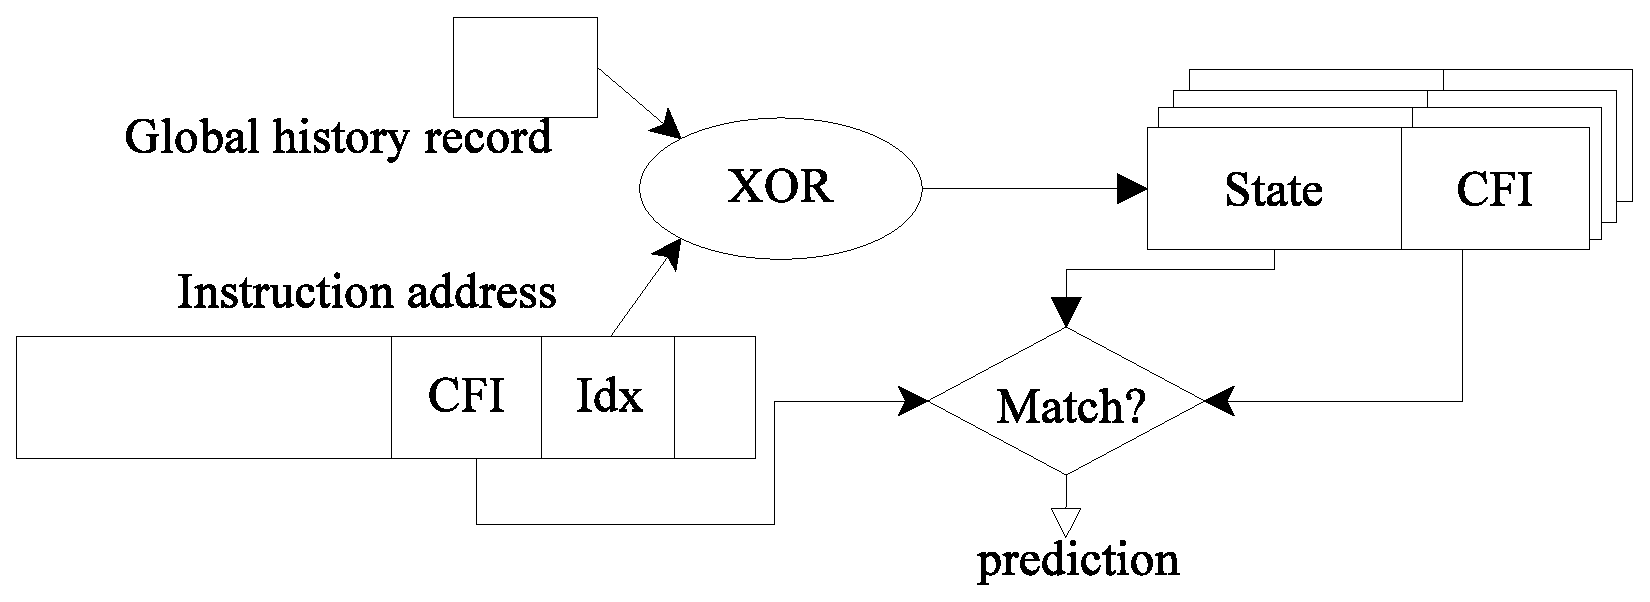
\includegraphics[width=\linewidth]{fig/dinome/gshare.eps}
\centering
\resizebox{0.7\linewidth}{!}{\protect\small% Graphic for TeX using PGF
% Title: /Users/ziqiaozhou/zzdiss/paper/fig/gshare.dia
% Creator: Dia v0.97.2
% CreationDate: Tue Jun 23 13:17:54 2020
% For: ziqiao
% \usepackage{tikz}
% The following commands are not supported in PSTricks at present
% We define them conditionally, so when they are implemented,
% this pgf file will use them.
\ifx\du\undefined
  \newlength{\du}
\fi
\setlength{\du}{11\unitlength}
\begin{tikzpicture}
\pgftransformxscale{1.000000}
\pgftransformyscale{-1.000000}
\definecolor{dialinecolor}{rgb}{0.000000, 0.000000, 0.000000}
\pgfsetstrokecolor{dialinecolor}
\definecolor{dialinecolor}{rgb}{1.000000, 1.000000, 1.000000}
\pgfsetfillcolor{dialinecolor}
\definecolor{dialinecolor}{rgb}{1.000000, 1.000000, 1.000000}
\pgfsetfillcolor{dialinecolor}
\fill (22.990082\du,10.143216\du)--(22.990082\du,11.547796\du)--(26.571524\du,11.547796\du)--(26.571524\du,10.143216\du)--cycle;
\pgfsetlinewidth{0.100000\du}
\pgfsetdash{}{0pt}
\pgfsetdash{}{0pt}
\pgfsetmiterjoin
\definecolor{dialinecolor}{rgb}{0.000000, 0.000000, 0.000000}
\pgfsetstrokecolor{dialinecolor}
\draw (22.990082\du,10.143216\du)--(22.990082\du,11.547796\du)--(26.571524\du,11.547796\du)--(26.571524\du,10.143216\du)--cycle;
% setfont left to latex
\definecolor{dialinecolor}{rgb}{0.000000, 0.000000, 0.000000}
\pgfsetstrokecolor{dialinecolor}
\node at (24.780803\du,11.056617\du){};
\definecolor{dialinecolor}{rgb}{1.000000, 1.000000, 1.000000}
\pgfsetfillcolor{dialinecolor}
\fill (26.559914\du,10.143016\du)--(26.559914\du,11.547796\du)--(29.758062\du,11.547796\du)--(29.758062\du,10.143016\du)--cycle;
\pgfsetlinewidth{0.100000\du}
\pgfsetdash{}{0pt}
\pgfsetdash{}{0pt}
\pgfsetmiterjoin
\definecolor{dialinecolor}{rgb}{0.000000, 0.000000, 0.000000}
\pgfsetstrokecolor{dialinecolor}
\draw (26.559914\du,10.143016\du)--(26.559914\du,11.547796\du)--(29.758062\du,11.547796\du)--(29.758062\du,10.143016\du)--cycle;
% setfont left to latex
\definecolor{dialinecolor}{rgb}{0.000000, 0.000000, 0.000000}
\pgfsetstrokecolor{dialinecolor}
\node at (28.158988\du,11.056517\du){};
\definecolor{dialinecolor}{rgb}{1.000000, 1.000000, 1.000000}
\pgfsetfillcolor{dialinecolor}
\fill (22.572803\du,10.417741\du)--(22.572803\du,11.822322\du)--(26.154245\du,11.822322\du)--(26.154245\du,10.417741\du)--cycle;
\pgfsetlinewidth{0.100000\du}
\pgfsetdash{}{0pt}
\pgfsetdash{}{0pt}
\pgfsetmiterjoin
\definecolor{dialinecolor}{rgb}{0.000000, 0.000000, 0.000000}
\pgfsetstrokecolor{dialinecolor}
\draw (22.572803\du,10.417741\du)--(22.572803\du,11.822322\du)--(26.154245\du,11.822322\du)--(26.154245\du,10.417741\du)--cycle;
% setfont left to latex
\definecolor{dialinecolor}{rgb}{0.000000, 0.000000, 0.000000}
\pgfsetstrokecolor{dialinecolor}
\node at (24.363524\du,11.331143\du){};
\definecolor{dialinecolor}{rgb}{1.000000, 1.000000, 1.000000}
\pgfsetfillcolor{dialinecolor}
\fill (26.142635\du,10.417541\du)--(26.142635\du,11.822322\du)--(29.340784\du,11.822322\du)--(29.340784\du,10.417541\du)--cycle;
\pgfsetlinewidth{0.100000\du}
\pgfsetdash{}{0pt}
\pgfsetdash{}{0pt}
\pgfsetmiterjoin
\definecolor{dialinecolor}{rgb}{0.000000, 0.000000, 0.000000}
\pgfsetstrokecolor{dialinecolor}
\draw (26.142635\du,10.417541\du)--(26.142635\du,11.822322\du)--(29.340784\du,11.822322\du)--(29.340784\du,10.417541\du)--cycle;
% setfont left to latex
\definecolor{dialinecolor}{rgb}{0.000000, 0.000000, 0.000000}
\pgfsetstrokecolor{dialinecolor}
\node at (27.741709\du,11.331043\du){};
\definecolor{dialinecolor}{rgb}{1.000000, 1.000000, 1.000000}
\pgfsetfillcolor{dialinecolor}
\fill (22.170165\du,10.740536\du)--(22.170165\du,12.145117\du)--(25.751607\du,12.145117\du)--(25.751607\du,10.740536\du)--cycle;
\pgfsetlinewidth{0.100000\du}
\pgfsetdash{}{0pt}
\pgfsetdash{}{0pt}
\pgfsetmiterjoin
\definecolor{dialinecolor}{rgb}{0.000000, 0.000000, 0.000000}
\pgfsetstrokecolor{dialinecolor}
\draw (22.170165\du,10.740536\du)--(22.170165\du,12.145117\du)--(25.751607\du,12.145117\du)--(25.751607\du,10.740536\du)--cycle;
% setfont left to latex
\definecolor{dialinecolor}{rgb}{0.000000, 0.000000, 0.000000}
\pgfsetstrokecolor{dialinecolor}
\node at (23.960886\du,11.653937\du){};
\definecolor{dialinecolor}{rgb}{1.000000, 1.000000, 1.000000}
\pgfsetfillcolor{dialinecolor}
\fill (25.739997\du,10.740336\du)--(25.739997\du,12.145117\du)--(28.938146\du,12.145117\du)--(28.938146\du,10.740336\du)--cycle;
\pgfsetlinewidth{0.100000\du}
\pgfsetdash{}{0pt}
\pgfsetdash{}{0pt}
\pgfsetmiterjoin
\definecolor{dialinecolor}{rgb}{0.000000, 0.000000, 0.000000}
\pgfsetstrokecolor{dialinecolor}
\draw (25.739997\du,10.740336\du)--(25.739997\du,12.145117\du)--(28.938146\du,12.145117\du)--(28.938146\du,10.740336\du)--cycle;
% setfont left to latex
\definecolor{dialinecolor}{rgb}{0.000000, 0.000000, 0.000000}
\pgfsetstrokecolor{dialinecolor}
\node at (27.339071\du,11.653837\du){};
% setfont left to latex
\definecolor{dialinecolor}{rgb}{0.000000, 0.000000, 0.000000}
\pgfsetstrokecolor{dialinecolor}
\node at (18.454000\du,9.857800\du){};
\definecolor{dialinecolor}{rgb}{1.000000, 1.000000, 1.000000}
\pgfsetfillcolor{dialinecolor}
\fill (16.107256\du,12.662545\du)--(18.452760\du,13.406780\du)--(16.107256\du,14.151015\du)--(13.761752\du,13.406780\du)--cycle;
\pgfsetlinewidth{0.180000\du}
\pgfsetdash{}{0pt}
\pgfsetdash{}{0pt}
\pgfsetmiterjoin
\definecolor{dialinecolor}{rgb}{0.000000, 0.000000, 0.000000}
\pgfsetstrokecolor{dialinecolor}
\draw (16.107256\du,12.662545\du)--(18.452760\du,13.406780\du)--(16.107256\du,14.151015\du)--(13.761752\du,13.406780\du)--cycle;
% setfont left to latex
\definecolor{dialinecolor}{rgb}{0.000000, 0.000000, 0.000000}
\pgfsetstrokecolor{dialinecolor}
\node at (16.107256\du,13.617892\du){};
% setfont left to latex
\definecolor{dialinecolor}{rgb}{0.000000, 0.000000, 0.000000}
\pgfsetstrokecolor{dialinecolor}
\node at (30.137432\du,16.256434\du){ prediction};
\definecolor{dialinecolor}{rgb}{1.000000, 1.000000, 1.000000}
\pgfsetfillcolor{dialinecolor}
\fill (21.928200\du,11.155200\du)--(21.928200\du,12.559780\du)--(25.509642\du,12.559780\du)--(25.509642\du,11.155200\du)--cycle;
\pgfsetlinewidth{0.100000\du}
\pgfsetdash{}{0pt}
\pgfsetdash{}{0pt}
\pgfsetmiterjoin
\definecolor{dialinecolor}{rgb}{0.000000, 0.000000, 0.000000}
\pgfsetstrokecolor{dialinecolor}
\draw (21.928200\du,11.155200\du)--(21.928200\du,12.559780\du)--(25.509642\du,12.559780\du)--(25.509642\du,11.155200\du)--cycle;
% setfont left to latex
\definecolor{dialinecolor}{rgb}{0.000000, 0.000000, 0.000000}
\pgfsetstrokecolor{dialinecolor}
\node at (23.718921\du,12.068601\du){};
\definecolor{dialinecolor}{rgb}{1.000000, 1.000000, 1.000000}
\pgfsetfillcolor{dialinecolor}
\fill (25.498032\du,11.155000\du)--(25.498032\du,12.559780\du)--(28.913760\du,12.559780\du)--(28.913760\du,11.155000\du)--cycle;
\pgfsetlinewidth{0.100000\du}
\pgfsetdash{}{0pt}
\pgfsetdash{}{0pt}
\pgfsetmiterjoin
\definecolor{dialinecolor}{rgb}{0.000000, 0.000000, 0.000000}
\pgfsetstrokecolor{dialinecolor}
\draw (25.498032\du,11.155000\du)--(25.498032\du,12.559780\du)--(28.913760\du,12.559780\du)--(28.913760\du,11.155000\du)--cycle;
% setfont left to latex
\definecolor{dialinecolor}{rgb}{0.000000, 0.000000, 0.000000}
\pgfsetstrokecolor{dialinecolor}
\node at (27.205896\du,12.068501\du){};
% setfont left to latex
\definecolor{dialinecolor}{rgb}{0.000000, 0.000000, 0.000000}
\pgfsetstrokecolor{dialinecolor}
\node at (23.718921\du,11.857490\du){CFI};
% setfont left to latex
\definecolor{dialinecolor}{rgb}{0.000000, 0.000000, 0.000000}
\pgfsetstrokecolor{dialinecolor}
\node at (27.205896\du,11.857390\du){state};
% setfont left to latex
\definecolor{dialinecolor}{rgb}{0.000000, 0.000000, 0.000000}
\pgfsetstrokecolor{dialinecolor}
\node at (25.457731\du,9.498925\du){GShare $\ACIFn{}(\textrm{`bpd'})$};
% setfont left to latex
\definecolor{dialinecolor}{rgb}{0.000000, 0.000000, 0.000000}
\pgfsetstrokecolor{dialinecolor}
\node at (19.094810\du,11.454096\du){\bpdIdx};
% setfont left to latex
\definecolor{dialinecolor}{rgb}{0.000000, 0.000000, 0.000000}
\pgfsetstrokecolor{dialinecolor}
\node at (25.417008\du,13.227528\du){untaken};
\pgfsetlinewidth{0.180000\du}
\pgfsetdash{}{0pt}
\pgfsetdash{}{0pt}
\pgfsetbuttcap
\pgfsetmiterjoin
\pgfsetlinewidth{0.180000\du}
\pgfsetbuttcap
\pgfsetmiterjoin
\pgfsetdash{}{0pt}
\definecolor{dialinecolor}{rgb}{1.000000, 1.000000, 1.000000}
\pgfsetfillcolor{dialinecolor}
\draw
(24.046019\du,14.540456\du)--(29.065995\du,14.540456\du)--(28.062000\du,15.726772\du)--(25.050014\du,15.726772\du)--(24.046019\du,14.540456\du)--cycle;
%\pgfpathmoveto{\pgfpoint{24.046019\du}{14.540456\du}}
%\pgfpathlineto{\pgfpoint{29.065995\du}{14.540456\du}}
%\pgfpathlineto{\pgfpoint{28.062000\du}{15.726772\du}}
%\pgfpathlineto{\pgfpoint{25.050014\du}{15.726772\du}}
%\pgfpathlineto{\pgfpoint{24.046019\du}{14.540456\du}}
%\pgfusepath{fill}
\definecolor{dialinecolor}{rgb}{0.000000, 0.000000, 0.000000}
\pgfsetstrokecolor{dialinecolor}
\draw
(24.046019\du,14.540456\du)--(29.065995\du,14.540456\du)--(28.062000\du,15.726772\du)--(25.050014\du,15.726772\du)--(24.046019\du,14.540456\du)--cycle;
%\pgfpathmoveto{\pgfpoint{24.046019\du}{14.540456\du}}
%\pgfpathlineto{\pgfpoint{29.065995\du}{14.540456\du}}
%\pgfpathlineto{\pgfpoint{28.062000\du}{15.726772\du}}
%\pgfpathlineto{\pgfpoint{25.050014\du}{15.726772\du}}
%\pgfpathlineto{\pgfpoint{24.046019\du}{14.540456\du}}
%\pgfusepath{stroke}
% setfont left to latex
\definecolor{dialinecolor}{rgb}{0.000000, 0.000000, 0.000000}
\pgfsetstrokecolor{dialinecolor}
\node at (26.556007\du,15.331169\du){};
\pgfsetlinewidth{0.100000\du}
\pgfsetdash{}{0pt}
\pgfsetdash{}{0pt}
\pgfsetmiterjoin
\pgfsetbuttcap
{
\definecolor{dialinecolor}{rgb}{0.000000, 0.000000, 0.000000}
\pgfsetfillcolor{dialinecolor}
% was here!!!
\pgfsetarrowsend{latex}
{\pgfsetcornersarced{\pgfpoint{0.000000\du}{0.000000\du}}\definecolor{dialinecolor}{rgb}{0.000000, 0.000000, 0.000000}
\pgfsetstrokecolor{dialinecolor}
\draw (16.107256\du,14.151015\du)--(16.107256\du,15.133614\du)--(24.548017\du,15.133614\du);
}}
\pgfsetlinewidth{0.100000\du}
\pgfsetdash{}{0pt}
\pgfsetdash{}{0pt}
\pgfsetmiterjoin
\pgfsetbuttcap
{
\definecolor{dialinecolor}{rgb}{0.000000, 0.000000, 0.000000}
\pgfsetfillcolor{dialinecolor}
% was here!!!
\pgfsetarrowsend{latex}
{\pgfsetcornersarced{\pgfpoint{0.000000\du}{0.000000\du}}\definecolor{dialinecolor}{rgb}{0.000000, 0.000000, 0.000000}
\pgfsetstrokecolor{dialinecolor}
\draw (23.718921\du,12.559780\du)--(23.718921\du,13.406780\du)--(18.452760\du,13.406780\du);
}}
% setfont left to latex
\definecolor{dialinecolor}{rgb}{0.000000, 0.000000, 0.000000}
\pgfsetstrokecolor{dialinecolor}
\node at (20.300610\du,14.650734\du){unmatch/match};
\pgfsetlinewidth{0.100000\du}
\pgfsetdash{}{0pt}
\pgfsetdash{}{0pt}
\pgfsetmiterjoin
\pgfsetbuttcap
{
\definecolor{dialinecolor}{rgb}{0.000000, 0.000000, 0.000000}
\pgfsetfillcolor{dialinecolor}
% was here!!!
\pgfsetarrowsend{latex}
{\pgfsetcornersarced{\pgfpoint{0.000000\du}{0.000000\du}}\definecolor{dialinecolor}{rgb}{0.000000, 0.000000, 0.000000}
\pgfsetstrokecolor{dialinecolor}
\draw (26.556007\du,15.726772\du)--(26.556007\du,16.223116\du)--(28.504550\du,16.223116\du);
}}
\pgfsetlinewidth{0.100000\du}
\pgfsetdash{}{0pt}
\pgfsetdash{}{0pt}
\pgfsetbuttcap
{
\definecolor{dialinecolor}{rgb}{0.000000, 0.000000, 0.000000}
\pgfsetfillcolor{dialinecolor}
% was here!!!
\pgfsetarrowsend{latex}
\definecolor{dialinecolor}{rgb}{0.000000, 0.000000, 0.000000}
\pgfsetstrokecolor{dialinecolor}
\draw (25.545504\du,13.566013\du)--(25.554156\du,14.443481\du);
}
\pgfsetlinewidth{0.100000\du}
\pgfsetdash{}{0pt}
\pgfsetdash{}{0pt}
\pgfsetbuttcap
{
\definecolor{dialinecolor}{rgb}{0.000000, 0.000000, 0.000000}
\pgfsetfillcolor{dialinecolor}
% was here!!!
\pgfsetarrowsend{latex}
\definecolor{dialinecolor}{rgb}{0.000000, 0.000000, 0.000000}
\pgfsetstrokecolor{dialinecolor}
\draw (27.205896\du,12.559780\du)--(27.206193\du,14.441649\du);
}
\pgfsetlinewidth{0.100000\du}
\pgfsetdash{}{0pt}
\pgfsetdash{}{0pt}
\pgfsetmiterjoin
\pgfsetbuttcap
{
\definecolor{dialinecolor}{rgb}{0.000000, 0.000000, 0.000000}
\pgfsetfillcolor{dialinecolor}
% was here!!!
\pgfsetarrowsend{latex}
{\pgfsetcornersarced{\pgfpoint{0.000000\du}{0.000000\du}}\definecolor{dialinecolor}{rgb}{0.000000, 0.000000, 0.000000}
\pgfsetstrokecolor{dialinecolor}
\draw (11.988491\du,11.354784\du)--(11.988491\du,13.406780\du)--(13.761752\du,13.406780\du);
}}
\pgfsetlinewidth{0.100000\du}
\pgfsetdash{{\pgflinewidth}{0.200000\du}}{0cm}
\pgfsetdash{{\pgflinewidth}{0.200000\du}}{0cm}
\pgfsetmiterjoin
\pgfsetbuttcap
{
\definecolor{dialinecolor}{rgb}{0.000000, 0.000000, 0.000000}
\pgfsetfillcolor{dialinecolor}
% was here!!!
\pgfsetarrowsend{latex}
{\pgfsetcornersarced{\pgfpoint{0.000000\du}{0.000000\du}}\definecolor{dialinecolor}{rgb}{0.000000, 0.000000, 0.000000}
\pgfsetstrokecolor{dialinecolor}
\draw (14.418341\du,11.354784\du)--(14.418341\du,11.857490\du)--(21.928200\du,11.857490\du);
}}
% setfont left to latex
\definecolor{dialinecolor}{rgb}{0.000000, 0.000000, 0.000000}
\pgfsetstrokecolor{dialinecolor}
\node at (12.785429\du,9.504472\du){Instruction address};
\definecolor{dialinecolor}{rgb}{1.000000, 1.000000, 1.000000}
\pgfsetfillcolor{dialinecolor}
\fill (8.222248\du,9.912439\du)--(8.222248\du,11.354784\du)--(10.715147\du,11.354784\du)--(10.715147\du,9.912439\du)--cycle;
\pgfsetlinewidth{0.100000\du}
\pgfsetdash{}{0pt}
\pgfsetdash{}{0pt}
\pgfsetmiterjoin
\definecolor{dialinecolor}{rgb}{0.000000, 0.000000, 0.000000}
\pgfsetstrokecolor{dialinecolor}
\draw (8.222248\du,9.912439\du)--(8.222248\du,11.354784\du)--(10.715147\du,11.354784\du)--(10.715147\du,9.912439\du)--cycle;
% setfont left to latex
\definecolor{dialinecolor}{rgb}{0.000000, 0.000000, 0.000000}
\pgfsetstrokecolor{dialinecolor}
\node at (9.468698\du,10.844722\du){};
\definecolor{dialinecolor}{rgb}{1.000000, 1.000000, 1.000000}
\pgfsetfillcolor{dialinecolor}
\fill (13.258341\du,9.912439\du)--(13.258341\du,11.354784\du)--(15.578341\du,11.354784\du)--(15.578341\du,9.912439\du)--cycle;
\pgfsetlinewidth{0.100000\du}
\pgfsetdash{}{0pt}
\pgfsetdash{}{0pt}
\pgfsetmiterjoin
\definecolor{dialinecolor}{rgb}{0.000000, 0.000000, 0.000000}
\pgfsetstrokecolor{dialinecolor}
\draw (13.258341\du,9.912439\du)--(13.258341\du,11.354784\du)--(15.578341\du,11.354784\du)--(15.578341\du,9.912439\du)--cycle;
% setfont left to latex
\definecolor{dialinecolor}{rgb}{0.000000, 0.000000, 0.000000}
\pgfsetstrokecolor{dialinecolor}
\node at (14.418341\du,10.844722\du){};
\definecolor{dialinecolor}{rgb}{1.000000, 1.000000, 1.000000}
\pgfsetfillcolor{dialinecolor}
\fill (15.509641\du,9.912439\du)--(15.509641\du,11.354784\du)--(16.872901\du,11.354784\du)--(16.872901\du,9.912439\du)--cycle;
\pgfsetlinewidth{0.100000\du}
\pgfsetdash{}{0pt}
\pgfsetdash{}{0pt}
\pgfsetmiterjoin
\definecolor{dialinecolor}{rgb}{0.000000, 0.000000, 0.000000}
\pgfsetstrokecolor{dialinecolor}
\draw (15.509641\du,9.912439\du)--(15.509641\du,11.354784\du)--(16.872901\du,11.354784\du)--(16.872901\du,9.912439\du)--cycle;
% setfont left to latex
\definecolor{dialinecolor}{rgb}{0.000000, 0.000000, 0.000000}
\pgfsetstrokecolor{dialinecolor}
\node at (16.191271\du,10.844722\du){};
\definecolor{dialinecolor}{rgb}{1.000000, 1.000000, 1.000000}
\pgfsetfillcolor{dialinecolor}
\fill (10.719741\du,9.914039\du)--(10.719741\du,11.354784\du)--(13.257241\du,11.354784\du)--(13.257241\du,9.914039\du)--cycle;
\pgfsetlinewidth{0.100000\du}
\pgfsetdash{}{0pt}
\pgfsetdash{}{0pt}
\pgfsetmiterjoin
\definecolor{dialinecolor}{rgb}{0.000000, 0.000000, 0.000000}
\pgfsetstrokecolor{dialinecolor}
\draw (10.719741\du,9.914039\du)--(10.719741\du,11.354784\du)--(13.257241\du,11.354784\du)--(13.257241\du,9.914039\du)--cycle;
% setfont left to latex
\definecolor{dialinecolor}{rgb}{0.000000, 0.000000, 0.000000}
\pgfsetstrokecolor{dialinecolor}
\node at (11.988491\du,10.845522\du){};
% setfont left to latex
\definecolor{dialinecolor}{rgb}{0.000000, 0.000000, 0.000000}
\pgfsetstrokecolor{dialinecolor}
\node at (11.988491\du,10.634411\du){CFI};
% setfont left to latex
\definecolor{dialinecolor}{rgb}{0.000000, 0.000000, 0.000000}
\pgfsetstrokecolor{dialinecolor}
\node at (14.418341\du,10.633611\du){idx};
% setfont left to latex
\definecolor{dialinecolor}{rgb}{0.000000, 0.000000, 0.000000}
\pgfsetstrokecolor{dialinecolor}
\node at (25.545504\du,15.026702\du){0};
% setfont left to latex
\definecolor{dialinecolor}{rgb}{0.000000, 0.000000, 0.000000}
\pgfsetstrokecolor{dialinecolor}
\node at (27.236388\du,15.026702\du){1};
\end{tikzpicture}
}
\caption{Logical architecture for GShare branch predictor}
\label{fig:gshare}
\end{figure}

\subsection{Logically modeling cache states}

The most common cache-based side-channel attacks are \primeprobe,
\flushreload, and their variants (e.g.,
see~\cite{zhang2012cross,yarom2014flush}).  In a \primeprobe attack,
the attacker loads memory blocks to fill (\Prime) cache sets, permits
the victim computation to run for a \primeprobe interval, and then
reads (\Probe{s}) these same blocks to determine which were evicted by
the victim computation during the \primeprobe interval.  In a
\flushreload attack, the attacker \Flush{es} a shared-memory block
from cache and then, after a \flushreload interval, accesses
(\Reload{s}) the block to determine whether the block was brought
back into the cache by the victim computation.

To model these attacks in our framework, it is necessary to model the
effects on the cache of the phases before victim execution (the \Prime
and \Flush steps) and to define \AOOFn{} to include the results of the
phases after victim execution (the \Probe and \Reload steps).  To do
so, we assume that the adversary has access to memory blocks
\block{1}, \block{2}, $\ldots$, \block{\blockNmbr} aligned to cache
lines, and we define the RISC-V assembly routine \accessProc by which
the adversary can access the block with index $\blockIdx =
\ACIFnAccess{}(\blockIdxVar)$ and empty \SecFnAccess{}:
\begin{center}
\begin{minipage}{0.6\columnwidth}
\begin{tabbing}
\accessProc(\ACIFnAccess{}, \AIIFnAccess{},  \SecFnAccess{}) \\
** \= ** \= \kill
\> \texttt{li s0, 0x2000000}\\ 
\> \texttt{add s1, s0, \blockIdx} \\
\> \texttt{sll s1, s1, 6}\\
\> \texttt{lbu a2, 0(s1)}
\end{tabbing}
\end{minipage}
\end{center}
Starting from hardware state \HwFnAccess{\blockIdx}{0}
($=~\AIIFnAccess{}$) that is completely symbolic, we generate the
per-cycle logical postcondition
$\TmpTransConstraints{\accessProc}(\HwFnAccess{\blockIdx}{\cycle-1},
\HwFnAccess{\blockIdx}{\cycle})$ for each $0 < \cycle \le
\ncyclesAccess$ as in \secref{dinome:sec:impl:logic}, where we empirically
choose $\ncyclesAccess = 45$.

We use these postconditions in two ways.  First, we use them to
extract a constraint
$\glueConstraints{}{}(\langle\HwFn{}{\cycle}\rangle_{\cycle=1}^{\ncycles},
\AOOFn{})$ that defines the attacker's observations \AOOFn{} in terms
of the hardware states
$\langle\HwFn{}{\cycle}\rangle_{\cycle=1}^{\ncycles}$ induced by the
execution (see~\eqnref{eqn:build-postcondition}). A naive attempt to
do so would be to simply include in \AOOFn{} the metadata for each
cache line at every step of the execution.  However, this would grant
too much power to an attacker, who should not be given access to the
tag values and the exact locations of blocks inside a set.  Instead,
we permit only a weaker attacker (cf., abstract
noninterference~\cite{giacobazzi2004abstract}) by defining the
constraint
$\glueConstraints{}{}(\langle\HwFn{}{\cycle}\rangle_{\cycle=1}^{\ncycles},\AOOFn{})$
that represents the view of cache hits and misses immediately
observable by the adversary, by:
\begin{align*}
  \AOOFn{}(\hitVar)[\blockIdx] = &
  \left(\begin{array}{ll}
    (\HwFnAccess{\blockIdx}{0} = \HwFn{}{\ncycles}) \wedge \left(\bigwedge_{\cycle
  = 1}^{\ncyclesAccess}
\TmpTransConstraints{\accessProc}(\HwFnAccess{\blockIdx}{\cycle-1},
\HwFnAccess{\blockIdx}{\cycle})\right) \\
\wedge~\hfill\left(1 - \bigvee_{\cycle = 1}^{\ncyclesAccess}
\cachemiss(\HwFnAccess{\blockIdx}{\cycle}, \block{\blockIdx})\right)
\end{array}\right)
\end{align*}
for $\blockIdx = \ACIFnAccess{}(\blockIdxVar)$.  Here, \cachemiss is a
\boom-defined Verilog code snippet that, intuitively, checks a set of
cache lines where \block{\blockIdx} might reside and returns $1$ (in a
register called \hitRegisterVar) if none of those cache lines has a
valid tag matched with \block{\blockIdx} (and returns $0$ otherwise).
In this way, we characterize the procedure \accessProc using a logical
postcondition without manually modeling \cachemiss.

Second, we permit the attacker to control which of its blocks are
loaded into the cache before the victim runs.  Specifically, the
predicate $\HwPostcondition{\proc}{0}(\ACIFn{}, \AIIFn{}, \SecFn{},
\HwFn{}{0})$ that controls the initial hardware state from which the
victim executes is modified to constrain which of the attacker's
blocks are present in cache, as communicated through a reserved
variable $\loadVar \in \ACIKeys$, for which the
$\ACIFn{}(\loadVar)$ is a bit vector of length \blockNmbr.  That is,
attacker block \block{\blockIdx} should be loaded before the victim
runs if and only if $\ACIFn{}(\loadVar)[\blockIdx] = 1$.  To effect
this in the $\HwPostcondition{\proc}{0}(\ACIFn{},
\AIIFn{}, \SecFn{}, \HwFn{}{0})$, we construct
$\HwPostcondition{\proc}{0}(\ACIFn{}, \AIIFn{}, \SecFn{}, \HwFn{}{0})$
to include
\begin{align*}
  \ACIFn{}(\loadVar)[\blockIdx] = &
  \left(\!\!\!\begin{array}{ll}
    (\HwFnAccess{\blockIdx}{0} = \HwFn{}{0}) \wedge \left(\bigwedge_{\cycle
  = 1}^{\ncyclesAccess}
\TmpTransConstraints{\accessProc}(\HwFnAccess{\blockIdx}{\cycle-1},
\HwFnAccess{\blockIdx}{\cycle})\right) \\
\wedge~\hfill\left(1 - \bigvee_{\cycle = 1}^{\ncyclesAccess}
\cachemiss(\HwFnAccess{\blockIdx}{\cycle}, \block{\blockIdx})\right)
\end{array}\!\!\!\right)
\end{align*}
Of course, we rename variables to ensure no conflicts between copies
of \HwFnAccess{\blockIdx}{\cycle} included within the
$\ACIFn{}(\loadVar)[\blockIdx]$ and $\AOOFn{}(\hitVar)[\blockIdx]$
constraints.

For an attacker, it is sufficient to control the cache using
$\blockNmbr=16$ blocks as the L1 data cache consists of only 16
cache lines in our experiments.

\subsection{Cache-based side channels}
\label{dinome:sec:exp:cache}

In this section, we evaluate cache-based side channels under different
memory isolation and cache configurations.

\subsubsection{Without shared memory}
\label{dinome:sec:exp:cache:normal:unshared}
\begin{figure}
\begin{subfigure}[t]{0.495\linewidth}
\resizebox{\linewidth}{!}{\protect\small% GNUPLOT: LaTeX picture with Postscript
\begingroup
  \fontfamily{Times-Roman}%
  \selectfont
  \makeatletter
  \providecommand\color[2][]{%
    \GenericError{(gnuplot) \space\space\space\@spaces}{%
      Package color not loaded in conjunction with
      terminal option `colourtext'%
    }{See the gnuplot documentation for explanation.%
    }{Either use 'blacktext' in gnuplot or load the package
      color.sty in LaTeX.}%
    \renewcommand\color[2][]{}%
  }%
  \providecommand\includegraphics[2][]{%
    \GenericError{(gnuplot) \space\space\space\@spaces}{%
      Package graphicx or graphics not loaded%
    }{See the gnuplot documentation for explanation.%
    }{The gnuplot epslatex terminal needs graphicx.sty or graphics.sty.}%
    \renewcommand\includegraphics[2][]{}%
  }%
  \providecommand\rotatebox[2]{#2}%
  \@ifundefined{ifGPcolor}{%
    \newif\ifGPcolor
    \GPcolortrue
  }{}%
  \@ifundefined{ifGPblacktext}{%
    \newif\ifGPblacktext
    \GPblacktexttrue
  }{}%
  % define a \g@addto@macro without @ in the name:
  \let\gplgaddtomacro\g@addto@macro
  % define empty templates for all commands taking text:
  \gdef\gplbacktext{}%
  \gdef\gplfronttext{}%
  \makeatother
  \ifGPblacktext
    % no textcolor at all
    \def\colorrgb#1{}%
    \def\colorgray#1{}%
  \else
    % gray or color?
    \ifGPcolor
      \def\colorrgb#1{\color[rgb]{#1}}%
      \def\colorgray#1{\color[gray]{#1}}%
      \expandafter\def\csname LTw\endcsname{\color{white}}%
      \expandafter\def\csname LTb\endcsname{\color{black}}%
      \expandafter\def\csname LTa\endcsname{\color{black}}%
      \expandafter\def\csname LT0\endcsname{\color[rgb]{1,0,0}}%
      \expandafter\def\csname LT1\endcsname{\color[rgb]{0,1,0}}%
      \expandafter\def\csname LT2\endcsname{\color[rgb]{0,0,1}}%
      \expandafter\def\csname LT3\endcsname{\color[rgb]{1,0,1}}%
      \expandafter\def\csname LT4\endcsname{\color[rgb]{0,1,1}}%
      \expandafter\def\csname LT5\endcsname{\color[rgb]{1,1,0}}%
      \expandafter\def\csname LT6\endcsname{\color[rgb]{0,0,0}}%
      \expandafter\def\csname LT7\endcsname{\color[rgb]{1,0.3,0}}%
      \expandafter\def\csname LT8\endcsname{\color[rgb]{0.5,0.5,0.5}}%
    \else
      % gray
      \def\colorrgb#1{\color{black}}%
      \def\colorgray#1{\color[gray]{#1}}%
      \expandafter\def\csname LTw\endcsname{\color{white}}%
      \expandafter\def\csname LTb\endcsname{\color{black}}%
      \expandafter\def\csname LTa\endcsname{\color{black}}%
      \expandafter\def\csname LT0\endcsname{\color{black}}%
      \expandafter\def\csname LT1\endcsname{\color{black}}%
      \expandafter\def\csname LT2\endcsname{\color{black}}%
      \expandafter\def\csname LT3\endcsname{\color{black}}%
      \expandafter\def\csname LT4\endcsname{\color{black}}%
      \expandafter\def\csname LT5\endcsname{\color{black}}%
      \expandafter\def\csname LT6\endcsname{\color{black}}%
      \expandafter\def\csname LT7\endcsname{\color{black}}%
      \expandafter\def\csname LT8\endcsname{\color{black}}%
    \fi
  \fi
    \setlength{\unitlength}{0.0500bp}%
    \ifx\gptboxheight\undefined%
      \newlength{\gptboxheight}%
      \newlength{\gptboxwidth}%
      \newsavebox{\gptboxtext}%
    \fi%
    \setlength{\fboxrule}{0.5pt}%
    \setlength{\fboxsep}{1pt}%
\begin{picture}(5040.00,3456.00)%
    \gplgaddtomacro\gplbacktext{%
      \csname LTb\endcsname%%
      \put(962,780){\makebox(0,0)[r]{\strut{}$0$}}%
      \put(962,1133){\makebox(0,0)[r]{\strut{}$0.2$}}%
      \put(962,1486){\makebox(0,0)[r]{\strut{}$0.4$}}%
      \put(962,1839){\makebox(0,0)[r]{\strut{}$0.6$}}%
      \put(962,2192){\makebox(0,0)[r]{\strut{}$0.8$}}%
      \put(962,2545){\makebox(0,0)[r]{\strut{}$1$}}%
      \put(1118,520){\makebox(0,0){\strut{}$0$}}%
      \put(2373,520){\makebox(0,0){\strut{}$1$}}%
      \put(3628,520){\makebox(0,0){\strut{}$2$}}%
      \put(4883,520){\makebox(0,0){\strut{}$3$}}%
    }%
    \gplgaddtomacro\gplfronttext{%
      \csname LTb\endcsname%%
      \put(309,1662){\rotatebox{-270}{\makebox(0,0){\strut{}\JaccardRand{\secretsSetSize}}}}%
      \put(3000,182){\makebox(0,0){\strut{}$\log_2{\secretsSetSize}$}}%
      \csname LTb\endcsname%%
      \put(1365,3161){\makebox(0,0)[l]{\strut{}$\cachesetNmbr=1$}}%
      \csname LTb\endcsname%%
      \put(1365,2849){\makebox(0,0)[l]{\strut{}$\cachesetNmbr=2$}}%
      \csname LTb\endcsname%%
      \put(2754,3161){\makebox(0,0)[l]{\strut{}$\cachesetNmbr=4$}}%
      \csname LTb\endcsname%%
      \put(2754,2849){\makebox(0,0)[l]{\strut{}$\cachesetNmbr=8$}}%
      \csname LTb\endcsname%%
      \put(4143,3161){\makebox(0,0)[l]{\strut{}$\cachesetNmbr=16$}}%
    }%
    \gplbacktext
    \put(0,0){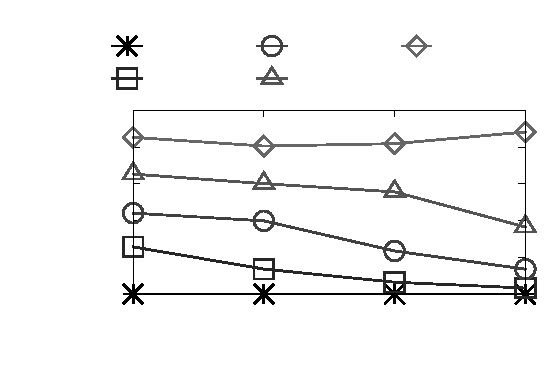
\includegraphics{normalunshared}}%
    \gplfronttext
  \end{picture}%
\endgroup
}
\caption{Symbolic $\ACIFn{}(\loadVar)$ \label{fig:normalcache:jaccard:unsharedsymload} }
\end{subfigure}%
\begin{subfigure}[t]{0.495\linewidth}
\resizebox{\linewidth}{!}{\protect\small% GNUPLOT: LaTeX picture with Postscript
\begingroup
  \fontfamily{Times-Roman}%
  \selectfont
  \makeatletter
  \providecommand\color[2][]{%
    \GenericError{(gnuplot) \space\space\space\@spaces}{%
      Package color not loaded in conjunction with
      terminal option `colourtext'%
    }{See the gnuplot documentation for explanation.%
    }{Either use 'blacktext' in gnuplot or load the package
      color.sty in LaTeX.}%
    \renewcommand\color[2][]{}%
  }%
  \providecommand\includegraphics[2][]{%
    \GenericError{(gnuplot) \space\space\space\@spaces}{%
      Package graphicx or graphics not loaded%
    }{See the gnuplot documentation for explanation.%
    }{The gnuplot epslatex terminal needs graphicx.sty or graphics.sty.}%
    \renewcommand\includegraphics[2][]{}%
  }%
  \providecommand\rotatebox[2]{#2}%
  \@ifundefined{ifGPcolor}{%
    \newif\ifGPcolor
    \GPcolortrue
  }{}%
  \@ifundefined{ifGPblacktext}{%
    \newif\ifGPblacktext
    \GPblacktexttrue
  }{}%
  % define a \g@addto@macro without @ in the name:
  \let\gplgaddtomacro\g@addto@macro
  % define empty templates for all commands taking text:
  \gdef\gplbacktext{}%
  \gdef\gplfronttext{}%
  \makeatother
  \ifGPblacktext
    % no textcolor at all
    \def\colorrgb#1{}%
    \def\colorgray#1{}%
  \else
    % gray or color?
    \ifGPcolor
      \def\colorrgb#1{\color[rgb]{#1}}%
      \def\colorgray#1{\color[gray]{#1}}%
      \expandafter\def\csname LTw\endcsname{\color{white}}%
      \expandafter\def\csname LTb\endcsname{\color{black}}%
      \expandafter\def\csname LTa\endcsname{\color{black}}%
      \expandafter\def\csname LT0\endcsname{\color[rgb]{1,0,0}}%
      \expandafter\def\csname LT1\endcsname{\color[rgb]{0,1,0}}%
      \expandafter\def\csname LT2\endcsname{\color[rgb]{0,0,1}}%
      \expandafter\def\csname LT3\endcsname{\color[rgb]{1,0,1}}%
      \expandafter\def\csname LT4\endcsname{\color[rgb]{0,1,1}}%
      \expandafter\def\csname LT5\endcsname{\color[rgb]{1,1,0}}%
      \expandafter\def\csname LT6\endcsname{\color[rgb]{0,0,0}}%
      \expandafter\def\csname LT7\endcsname{\color[rgb]{1,0.3,0}}%
      \expandafter\def\csname LT8\endcsname{\color[rgb]{0.5,0.5,0.5}}%
    \else
      % gray
      \def\colorrgb#1{\color{black}}%
      \def\colorgray#1{\color[gray]{#1}}%
      \expandafter\def\csname LTw\endcsname{\color{white}}%
      \expandafter\def\csname LTb\endcsname{\color{black}}%
      \expandafter\def\csname LTa\endcsname{\color{black}}%
      \expandafter\def\csname LT0\endcsname{\color{black}}%
      \expandafter\def\csname LT1\endcsname{\color{black}}%
      \expandafter\def\csname LT2\endcsname{\color{black}}%
      \expandafter\def\csname LT3\endcsname{\color{black}}%
      \expandafter\def\csname LT4\endcsname{\color{black}}%
      \expandafter\def\csname LT5\endcsname{\color{black}}%
      \expandafter\def\csname LT6\endcsname{\color{black}}%
      \expandafter\def\csname LT7\endcsname{\color{black}}%
      \expandafter\def\csname LT8\endcsname{\color{black}}%
    \fi
  \fi
    \setlength{\unitlength}{0.0500bp}%
    \ifx\gptboxheight\undefined%
      \newlength{\gptboxheight}%
      \newlength{\gptboxwidth}%
      \newsavebox{\gptboxtext}%
    \fi%
    \setlength{\fboxrule}{0.5pt}%
    \setlength{\fboxsep}{1pt}%
\begin{picture}(5040.00,3456.00)%
    \gplgaddtomacro\gplbacktext{%
      \csname LTb\endcsname%%
      \put(962,780){\makebox(0,0)[r]{\strut{}$0$}}%
      \put(962,1133){\makebox(0,0)[r]{\strut{}$0.2$}}%
      \put(962,1486){\makebox(0,0)[r]{\strut{}$0.4$}}%
      \put(962,1839){\makebox(0,0)[r]{\strut{}$0.6$}}%
      \put(962,2192){\makebox(0,0)[r]{\strut{}$0.8$}}%
      \put(962,2545){\makebox(0,0)[r]{\strut{}$1$}}%
      \put(1118,520){\makebox(0,0){\strut{}$0$}}%
      \put(2373,520){\makebox(0,0){\strut{}$1$}}%
      \put(3628,520){\makebox(0,0){\strut{}$2$}}%
      \put(4883,520){\makebox(0,0){\strut{}$3$}}%
    }%
    \gplgaddtomacro\gplfronttext{%
      \csname LTb\endcsname%%
      \put(309,1662){\rotatebox{-270}{\makebox(0,0){\strut{}\JaccardRand{\secretsSetSize}}}}%
      \put(3000,182){\makebox(0,0){\strut{}$\log_2{\secretsSetSize}$}}%
      \csname LTb\endcsname%%
      \put(1365,3161){\makebox(0,0)[l]{\strut{}$\cachesetNmbr=1$}}%
      \csname LTb\endcsname%%
      \put(1365,2849){\makebox(0,0)[l]{\strut{}$\cachesetNmbr=2$}}%
      \csname LTb\endcsname%%
      \put(2754,3161){\makebox(0,0)[l]{\strut{}$\cachesetNmbr=4$}}%
      \csname LTb\endcsname%%
      \put(2754,2849){\makebox(0,0)[l]{\strut{}$\cachesetNmbr=8$}}%
      \csname LTb\endcsname%%
      \put(4143,3161){\makebox(0,0)[l]{\strut{}$\cachesetNmbr=16$}}%
    }%
    \gplbacktext
    \put(0,0){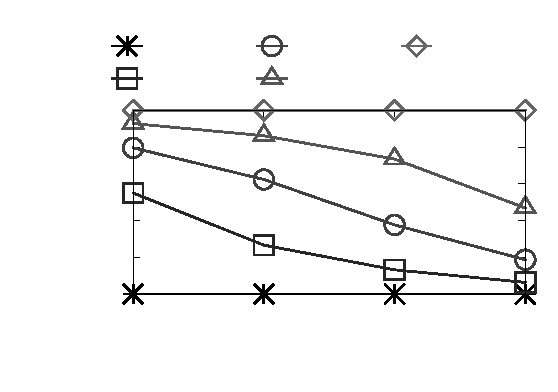
\includegraphics{normalprimeprobe}}%
    \gplfronttext
  \end{picture}%
\endgroup
}
\caption{$\forall \blockIdx: \ACIFn{}(\loadVar)[\blockIdx] = 1$ }
\label{fig:normalcache:jaccard:prime}
\end{subfigure}%
\caption{\JaccardRand{\secretsSetSize} for \primeprobe attacks}
\label{fig:normalcache:jaccard:unshared}
\end{figure}
\setlength{\tabcolsep}{0.3ex}
\renewcommand{\arraystretch}{1.3}

\iffalse
\begin{table}
\caption{An rule for \interferenceSet{} in a 2-way 8-set cache w/o shared memory
 \label{tab:s8w2:unshared}}
\vspace{-1ex}
%(depth=8, ntree=64)
\scriptsize{
\begingroup
\everymath{\scriptstyle}
\footnotesize
%your equation
\begin{tabular}{m{\colR}m{\colRule}m{\colPrecision}m{\colRecall}}
\toprule
 & Interference Rule (\interferenceRule{}) & Precision & Recall \\
\midrule
$\interferenceRule{0}$&$\SecFn{}(\secretVar)[2]\ge 1 \wedge
\SecFn{}(\secretVar)[1]< 1 \wedge \SecFn{}(\secretVar)[0]\ge 1 \wedge
\SecFnAlt{}(\secretVar)[1]\ge 1 \wedge \ACIFn{}(\loadVar)[5]\ge 1
\wedge \ACIFn{}(\loadVar)[13]\ge 1$&1.00&0.04\\
\if0
$\interferenceRule{1}$&$\diffFeature{0}\ge 1 \wedge
\SecFn{}(\secretVar)[2]< 1 \wedge \SecFn{}(\secretVar)[1]\ge 1 \wedge
\SecFn{}(\secretVar)[0]\ge 1 \wedge \ACIFn{}(\loadVar)[3]\ge 1 \wedge
\ACIFn{}(\loadVar)[11]\ge 1$&1.00&0.04\\
$\interferenceRule{2}$&$\SecFn{}(\secretVar)\ge 2 \wedge
\SecFnAlt{}(\text{`secret})\ge 9 \wedge \SecFnAlt{}(\text{`secret})< 10
\wedge \ACIFn{}(\loadVar)[9]\ge 1 \wedge \ACIFn{}(\loadVar)[1]\ge
1$&1.00&0.03\\ $\interferenceRule{3}$&$\SecFn{}(\secretVar)\ge 3
\wedge \SecFnAlt{}(\text{`secret})\ge 10 \wedge
\SecFnAlt{}(\text{`secret})< 11 \wedge \ACIFn{}(\loadVar)[2]\ge 1
\wedge \ACIFn{}(\loadVar)[10]\ge 1$&1.00&0.03\\
$\interferenceRule{4}$&$\SecFn{}(\secretVar)\ge 4 \wedge
\SecFnAlt{}(\text{`secret})\ge 11 \wedge \SecFnAlt{}(\secretVar)[2]< 1
\wedge \ACIFn{}(\loadVar)[3]\ge 1 \wedge \ACIFn{}(\loadVar)[11]\ge
1$&1.00&0.03\\ $\interferenceRule{5}$&$\SecFn{}(\secretVar)[0]\ge 1
\wedge \SecFnAlt{}(\text{`secret})< 1 \wedge \ACIFn{}(\loadVar)[8]\ge 1
\wedge \ACIFn{}(\loadVar)[0]\ge 1$&1.00&0.02\\
\fi
\bottomrule
\end{tabular}
\endgroup
}
\vspace{1.5ex}
\caption{Rules for \noninterferenceSet{} for 2-way 8-set cache w/o
memory sharing
\vspace{-1ex}
\label{tab:s8w2:unshared:noninterference}}
\scriptsize{
\begingroup
\everymath{\scriptstyle}
\footnotesize
%your equation
\begin{tabular}{m{\colR}m{\colRule}m{\colPrecision}m{\colRecall}}
\toprule
 & Noninterference rule (\noninterferenceRule{}) & Precision & Recall \\
\midrule
$\noninterferenceRule{0}$&$\diffFeature{2}< 1 \wedge \diffFeature{1}< 1 \wedge \diffFeature{0}< 1$&1.00&0.11\\
\if
$\interferenceRule{1}$&$\SecFn{}(\secretVar)[2]\ge 1 \wedge
\SecFn{}(\secretVar)[0]\ge 1 \wedge \SecFnAlt{}(\secretVar)[2]\ge 1
\wedge \SecFnAlt{}(\secretVar)[0]\ge 1 \wedge \ACIFn{}(\loadVar)[15]< 1 \wedge \ACIFn{}(\loadVar)[13]< 1$&1.00&0.02\\
$\interferenceRule{2}$&$\diffFeature{2}< 1 \wedge \diffFeature{0}< 1 \wedge \SecFn{}(\secretVar)[2]\ge 1 \wedge \SecFn{}(\secretVar)[0]< 1 \wedge \ACIFn{}(\loadVar)[6]< 1 \wedge \ACIFn{}(\loadVar)[12]< 1$&1.00&0.02\\
$\interferenceRule{3}$&$\SecFn{}(\secretVar)[2]\ge 1 \wedge \SecFn{}(\secretVar)[1]\ge 1 \wedge \SecFnAlt{}(\text{`secret})\ge 3 \wedge \SecFnAlt{}(\secretVar)[1]\ge 1 \wedge \ACIFn{}(\loadVar)[7]< 1 \wedge \ACIFn{}(\loadVar)[14]< 1 \wedge \ACIFn{}(\loadVar)[11]< 1$&0.94&0.02\\
$\interferenceRule{4}$&$\diffFeature{2}\ge 1 \wedge \diffFeature{1}\ge 1 \wedge \SecFn{}(\secretVar)\ge 2 \wedge \SecFn{}(\secretVar)< 6 \wedge \ACIFn{}(\loadVar)[5]< 1 \wedge \ACIFn{}(\loadVar)[11]< 1 \wedge \ACIFn{}(\loadVar)[10]< 1$&0.83&0.01\\
$\interferenceRule{5}$&$\diffFeature{2}\ge 1 \wedge \diffFeature{0}\ge 1 \wedge \SecFn{}(\secretVar)\ge 3 \wedge \SecFn{}(\secretVar)[1]\ge 1 \wedge \SecFn{}(\secretVar)< 7 \wedge \ACIFn{}(\loadVar)[6]< 1 \wedge \ACIFn{}(\loadVar)[3]< 1$&0.83&0.01\\
$\interferenceRule{6}$&$\diffFeature{2}< 1 \wedge \SecFn{}(\secretVar)\ge 1 \wedge \SecFn{}(\secretVar)[2]< 1 \wedge \SecFnAlt{}(\secretVar)[1]\ge 1 \wedge \ACIFn{}(\loadVar)[3]< 1 \wedge \ACIFn{}(\loadVar)[2]< 1$&0.83&0.04\\
$\interferenceRule{7}$&$\SecFn{}(\secretVar)[2]< 1 \wedge \SecFn{}(\secretVar)[1]< 1 \wedge \SecFn{}(\secretVar)[0]< 1 \wedge \SecFnAlt{}(\secretVar)[2]\ge 1 \wedge \SecFnAlt{}(\secretVar)[0]\ge 1 \wedge \ACIFn{}(\loadVar)[5]< 1 \wedge \ACIFn{}(\loadVar)[0]< 1$&0.83&0.01\\
$\interferenceRule{8}$&$\SecFn{}(\secretVar)[2]\ge 1 \wedge \SecFn{}(\secretVar)[1]< 1 \wedge \SecFnAlt{}(\text{`secret})\ge 2 \wedge \SecFnAlt{}(\text{`secret})< 6 \wedge \ACIFn{}(\loadVar)[5]< 1 \wedge \ACIFn{}(\loadVar)[4]< 1$&0.80&0.02\\
$\interferenceRule{9}$&$\SecFn{}(\secretVar)[2]\ge 1 \wedge \SecFn{}(\secretVar)[1]< 1 \wedge \ACIFn{}(\loadVar)[4]< 1 \wedge \ACIFn{}(\loadVar)[2]< 1 \wedge \ACIFn{}(\loadVar)[13]< 1$&0.78&0.04\\
\fi
\bottomrule
\end{tabular}
\endgroup
}
\end{table} 
\fi

Here, we target a victim's RISC-V assembly \proc to access a
secret-indexed memory block not shared with the attacker, by setting
the base address in \texttt{s0} to a value \texttt{0x2000010}, in
contrast to the one used in \accessProc.
\begin{align}
\begin{minipage}{0.6\columnwidth}
\begin{tabbing}
\proc(\ACIFn{}, \AIIFn{}, \SecFn{}) \\
** \= ** \= \kill
\> \texttt{li s0, 0x2000010}\\ 
\> \texttt{add s1, s0, $\SecFn{}(\secretVar)$} \\
\> \texttt{sll s1, s1, 6}\\
\> \texttt{lbu a2, 0(s1)}
\end{tabbing}
\end{minipage}
\label{eqn:proc}
\end{align}

We experimented with different numbers of cache sets \cachesetNmbr
including $\cachesetNmbr=1$ (i.e., 1-way, 16-set, fully associative),
$\cachesetNmbr=2$ (i.e., 8-way, 2-set), $\cachesetNmbr=4$ (i.e., 4-way,
4-set), $\cachesetNmbr=8$ (2-way, 8-set), and $\cachesetNmbr=16$ (i.e.,
1-way, 16-set, direct-mapped). As shown in
\figref{fig:normalcache:jaccard:unsharedsymload},
\JaccardRand{\secretsSetSize} increases when the number of sets
increases.  Specifically, there is no leakage
($\JaccardRand{\secretsSetSize} = 0$ for all \secretsSetSize) when
$\cachesetNmbr=1$. Using fewer cache sets, each cache set is shared by
more memory blocks, and so an attacker will have more difficulty
distinguishing one execution from others. When $1 < \cachesetNmbr <
16$, \JaccardRand{\secretsSetSize} decreases as \secretsSetSize grows,
since the attacker can learn only $log_2(\cachesetNmbr)$ bits about the
secret and thus may be unable to distinguish secrets in large sets
(i.e., large \secretsSetSize).

An example \textit{interference} rule for \interferenceSet generated
as described in \secref{dinome:sec:interpret} with the highest precision
(1.00) and a recall $\approx 0.04$ in a 2-way, 8-set cache is:
\begin{align}
  \begin{array}{rrrr}
    & \SecFn{}(\secretVar)[2]\ge 1 & \wedge & \SecFn{}(\secretVar)[1]< 1 \\
    \wedge & \SecFn{}(\secretVar)[0]\ge 1 & \wedge & \SecFnAlt{}(\secretVar)[1]\ge 1 \\
    \wedge & \ACIFn{}(\loadVar)[5]\ge 1   & \wedge & \ACIFn{}(\loadVar)[13]\ge 1
  \end{array}
  \label{eqn:prime-probe-interference}
\end{align}
In this rule, the \SecFn{} and \SecFnAlt{} conjuncts concretize the
least significant 3 bits of $\SecFn{}(\secretVar)$ (i.e.,
$\SecFn{}(\secretVar) \equiv 5 \bmod 8$) and the lowest bit of
$\SecFnAlt{}(\secretVar)$ (i.e., $\SecFnAlt{}(\secretVar) \equiv 0 \bmod 2$). The \ACIFn{} conjuncts are $\ACIFn{}(\loadVar)[5]\ge 1$ and
$\ACIFn{}(\loadVar)[13]\ge 1$; note that $13\equiv 5 \bmod 8$. That
is, an attacker could load all blocks \block{\blockIdx} with
$\blockIdx \equiv 5 \bmod 8$ into cache to distinguish a secret
$\SecFn{}(\secretVar) \equiv 5 \bmod 8$ from $\SecFnAlt{}(\secretVar)
\bmod 8 \in \{0,2,4,6\}$.

Our approach could not directly represent
$\ACIFn{}(\loadVar)[\blockIdx] \equiv \SecFn{}(\secretVar) \bmod
\cachesetNmbr$.  So, the trees in the model split the dataset based on
the cache set index.  As such, there were many other top-ranking rules
similar to \eqnref{eqn:prime-probe-interference}, each focusing on one
residue class of the secret value modulo \cachesetNmbr where
$\cachesetNmbr=8$ and constraining $\ACIFn{}(\loadVar)[\blockIdx] = 1$
for all \blockIdx with that residue class modulo \cachesetNmbr.  Each
such rule works for $\frac{1}{8}$ of \SecFn{}'s domain and
$\frac{1}{2}$ of \SecFnAlt{}'s domain, thus only for
$\frac{1}{8}\times\frac{1}{2}\approx0.06$ of secret pairs. The recall
rate $0.04 < 0.06$ indicates that priming the corresponding cache set
ensures (i.e., precision $=~1.0$) the interference but is not
necessary to cause it.

Analogously, we can generate rules for the \textit{noninterference}
set \noninterferenceSet, as well.  One example with precision 1.0
(i.e., that ensures noninterference) and recall 0.11 constrains the
secret's least-significant 3 bits to be the same for \SecFn{} and
\SecFnAlt{}:
\begin{align}
  \begin{array}{rr}
  & \diffFeature{2}< 1 \\
  \wedge & \diffFeature{1}< 1 \\
  \wedge & \diffFeature{0}< 1
  \end{array}
  \label{eqn:prime-probe-noninterference}
\end{align}
This analysis illustrates that an attacker can easily distinguish
$\SecFn{}(\secretVar)$ and $\SecFnAlt{}(\secretVar)$ when priming a
cache set used by $\SecFn{}(\secretVar)$ or $\SecFnAlt{}(\secretVar)$
but not both.  It is therefore safe to assume that the attacker will
\Prime the cache using all its controlled memory blocks to maximize
the chances for leakage.  The \JaccardRand{ \secretsSetSize} measure
under this specific attack is shown in
\figref{fig:normalcache:jaccard:prime}. The worst case will leak all
of the 4-bit secret when using high-granularity memory-to-cache
mapping, i.e., where $\cachesetNmbr=16$.

\if
For
example, an attacker could partially fill one cache set by only set
$\ACIFn{}(\loadVar)[5]\ge 1$, then he still have some chance to observe
the cache miss caused by the victim with a random replacement policy.
\fi
 
\subsubsection{With shared memory}

\begin{figure}
\begin{subfigure}[t]{0.495\linewidth}
\resizebox{\linewidth}{!}{\protect\small% GNUPLOT: LaTeX picture with Postscript
\begingroup
  \fontfamily{Times-Roman}%
  \selectfont
  \makeatletter
  \providecommand\color[2][]{%
    \GenericError{(gnuplot) \space\space\space\@spaces}{%
      Package color not loaded in conjunction with
      terminal option `colourtext'%
    }{See the gnuplot documentation for explanation.%
    }{Either use 'blacktext' in gnuplot or load the package
      color.sty in LaTeX.}%
    \renewcommand\color[2][]{}%
  }%
  \providecommand\includegraphics[2][]{%
    \GenericError{(gnuplot) \space\space\space\@spaces}{%
      Package graphicx or graphics not loaded%
    }{See the gnuplot documentation for explanation.%
    }{The gnuplot epslatex terminal needs graphicx.sty or graphics.sty.}%
    \renewcommand\includegraphics[2][]{}%
  }%
  \providecommand\rotatebox[2]{#2}%
  \@ifundefined{ifGPcolor}{%
    \newif\ifGPcolor
    \GPcolortrue
  }{}%
  \@ifundefined{ifGPblacktext}{%
    \newif\ifGPblacktext
    \GPblacktexttrue
  }{}%
  % define a \g@addto@macro without @ in the name:
  \let\gplgaddtomacro\g@addto@macro
  % define empty templates for all commands taking text:
  \gdef\gplbacktext{}%
  \gdef\gplfronttext{}%
  \makeatother
  \ifGPblacktext
    % no textcolor at all
    \def\colorrgb#1{}%
    \def\colorgray#1{}%
  \else
    % gray or color?
    \ifGPcolor
      \def\colorrgb#1{\color[rgb]{#1}}%
      \def\colorgray#1{\color[gray]{#1}}%
      \expandafter\def\csname LTw\endcsname{\color{white}}%
      \expandafter\def\csname LTb\endcsname{\color{black}}%
      \expandafter\def\csname LTa\endcsname{\color{black}}%
      \expandafter\def\csname LT0\endcsname{\color[rgb]{1,0,0}}%
      \expandafter\def\csname LT1\endcsname{\color[rgb]{0,1,0}}%
      \expandafter\def\csname LT2\endcsname{\color[rgb]{0,0,1}}%
      \expandafter\def\csname LT3\endcsname{\color[rgb]{1,0,1}}%
      \expandafter\def\csname LT4\endcsname{\color[rgb]{0,1,1}}%
      \expandafter\def\csname LT5\endcsname{\color[rgb]{1,1,0}}%
      \expandafter\def\csname LT6\endcsname{\color[rgb]{0,0,0}}%
      \expandafter\def\csname LT7\endcsname{\color[rgb]{1,0.3,0}}%
      \expandafter\def\csname LT8\endcsname{\color[rgb]{0.5,0.5,0.5}}%
    \else
      % gray
      \def\colorrgb#1{\color{black}}%
      \def\colorgray#1{\color[gray]{#1}}%
      \expandafter\def\csname LTw\endcsname{\color{white}}%
      \expandafter\def\csname LTb\endcsname{\color{black}}%
      \expandafter\def\csname LTa\endcsname{\color{black}}%
      \expandafter\def\csname LT0\endcsname{\color{black}}%
      \expandafter\def\csname LT1\endcsname{\color{black}}%
      \expandafter\def\csname LT2\endcsname{\color{black}}%
      \expandafter\def\csname LT3\endcsname{\color{black}}%
      \expandafter\def\csname LT4\endcsname{\color{black}}%
      \expandafter\def\csname LT5\endcsname{\color{black}}%
      \expandafter\def\csname LT6\endcsname{\color{black}}%
      \expandafter\def\csname LT7\endcsname{\color{black}}%
      \expandafter\def\csname LT8\endcsname{\color{black}}%
    \fi
  \fi
    \setlength{\unitlength}{0.0500bp}%
    \ifx\gptboxheight\undefined%
      \newlength{\gptboxheight}%
      \newlength{\gptboxwidth}%
      \newsavebox{\gptboxtext}%
    \fi%
    \setlength{\fboxrule}{0.5pt}%
    \setlength{\fboxsep}{1pt}%
\begin{picture}(5616.00,3310.00)%
    \gplgaddtomacro\gplbacktext{%
      \csname LTb\endcsname%%
      \put(962,780){\makebox(0,0)[r]{\strut{}$0$}}%
      \put(962,1260){\makebox(0,0)[r]{\strut{}$0.2$}}%
      \put(962,1740){\makebox(0,0)[r]{\strut{}$0.4$}}%
      \put(962,2219){\makebox(0,0)[r]{\strut{}$0.6$}}%
      \put(962,2699){\makebox(0,0)[r]{\strut{}$0.8$}}%
      \put(962,3179){\makebox(0,0)[r]{\strut{}$1$}}%
      \put(1118,520){\makebox(0,0){\strut{}$0$}}%
      \put(2565,520){\makebox(0,0){\strut{}$1$}}%
      \put(4012,520){\makebox(0,0){\strut{}$2$}}%
      \put(5459,520){\makebox(0,0){\strut{}$3$}}%
    }%
    \gplgaddtomacro\gplfronttext{%
      \csname LTb\endcsname%%
      \put(309,1979){\rotatebox{-270}{\makebox(0,0){\strut{}\JaccardRand{\secretsSetSize}}}}%
      \put(3288,182){\makebox(0,0){\strut{}$\log_2{\secretsSetSize}$}}%
      \csname LTb\endcsname%%
      \put(1883,1350){\makebox(0,0)[l]{\strut{}$\cachesetNmbr=1$}}%
      \csname LTb\endcsname%%
      \put(1883,1012){\makebox(0,0)[l]{\strut{}$\cachesetNmbr=2$}}%
      \csname LTb\endcsname%%
      \put(3272,1350){\makebox(0,0)[l]{\strut{}$\cachesetNmbr=4$}}%
      \csname LTb\endcsname%%
      \put(3272,1012){\makebox(0,0)[l]{\strut{}$\cachesetNmbr=8$}}%
      \csname LTb\endcsname%%
      \put(4661,1350){\makebox(0,0)[l]{\strut{}$\cachesetNmbr=16$}}%
    }%
    \gplbacktext
    \put(0,0){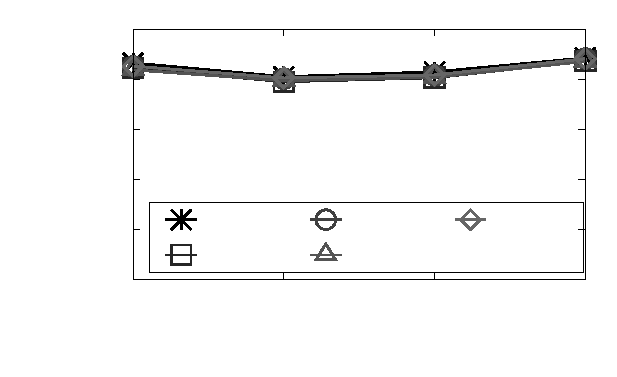
\includegraphics{normalshared}}%
    \gplfronttext
  \end{picture}%
\endgroup
}
\caption{Symbolic $\ACIFn{}(\loadVar)$ \label{fig:normalcache:jaccard:sharedsymloads}
}
\end{subfigure}%
\begin{subfigure}[t]{0.495\linewidth}
\resizebox{\linewidth}{!}{\protect\small% GNUPLOT: LaTeX picture with Postscript
\begingroup
  \fontfamily{Times-Roman}%
  \selectfont
  \makeatletter
  \providecommand\color[2][]{%
    \GenericError{(gnuplot) \space\space\space\@spaces}{%
      Package color not loaded in conjunction with
      terminal option `colourtext'%
    }{See the gnuplot documentation for explanation.%
    }{Either use 'blacktext' in gnuplot or load the package
      color.sty in LaTeX.}%
    \renewcommand\color[2][]{}%
  }%
  \providecommand\includegraphics[2][]{%
    \GenericError{(gnuplot) \space\space\space\@spaces}{%
      Package graphicx or graphics not loaded%
    }{See the gnuplot documentation for explanation.%
    }{The gnuplot epslatex terminal needs graphicx.sty or graphics.sty.}%
    \renewcommand\includegraphics[2][]{}%
  }%
  \providecommand\rotatebox[2]{#2}%
  \@ifundefined{ifGPcolor}{%
    \newif\ifGPcolor
    \GPcolortrue
  }{}%
  \@ifundefined{ifGPblacktext}{%
    \newif\ifGPblacktext
    \GPblacktexttrue
  }{}%
  % define a \g@addto@macro without @ in the name:
  \let\gplgaddtomacro\g@addto@macro
  % define empty templates for all commands taking text:
  \gdef\gplbacktext{}%
  \gdef\gplfronttext{}%
  \makeatother
  \ifGPblacktext
    % no textcolor at all
    \def\colorrgb#1{}%
    \def\colorgray#1{}%
  \else
    % gray or color?
    \ifGPcolor
      \def\colorrgb#1{\color[rgb]{#1}}%
      \def\colorgray#1{\color[gray]{#1}}%
      \expandafter\def\csname LTw\endcsname{\color{white}}%
      \expandafter\def\csname LTb\endcsname{\color{black}}%
      \expandafter\def\csname LTa\endcsname{\color{black}}%
      \expandafter\def\csname LT0\endcsname{\color[rgb]{1,0,0}}%
      \expandafter\def\csname LT1\endcsname{\color[rgb]{0,1,0}}%
      \expandafter\def\csname LT2\endcsname{\color[rgb]{0,0,1}}%
      \expandafter\def\csname LT3\endcsname{\color[rgb]{1,0,1}}%
      \expandafter\def\csname LT4\endcsname{\color[rgb]{0,1,1}}%
      \expandafter\def\csname LT5\endcsname{\color[rgb]{1,1,0}}%
      \expandafter\def\csname LT6\endcsname{\color[rgb]{0,0,0}}%
      \expandafter\def\csname LT7\endcsname{\color[rgb]{1,0.3,0}}%
      \expandafter\def\csname LT8\endcsname{\color[rgb]{0.5,0.5,0.5}}%
    \else
      % gray
      \def\colorrgb#1{\color{black}}%
      \def\colorgray#1{\color[gray]{#1}}%
      \expandafter\def\csname LTw\endcsname{\color{white}}%
      \expandafter\def\csname LTb\endcsname{\color{black}}%
      \expandafter\def\csname LTa\endcsname{\color{black}}%
      \expandafter\def\csname LT0\endcsname{\color{black}}%
      \expandafter\def\csname LT1\endcsname{\color{black}}%
      \expandafter\def\csname LT2\endcsname{\color{black}}%
      \expandafter\def\csname LT3\endcsname{\color{black}}%
      \expandafter\def\csname LT4\endcsname{\color{black}}%
      \expandafter\def\csname LT5\endcsname{\color{black}}%
      \expandafter\def\csname LT6\endcsname{\color{black}}%
      \expandafter\def\csname LT7\endcsname{\color{black}}%
      \expandafter\def\csname LT8\endcsname{\color{black}}%
    \fi
  \fi
    \setlength{\unitlength}{0.0500bp}%
    \ifx\gptboxheight\undefined%
      \newlength{\gptboxheight}%
      \newlength{\gptboxwidth}%
      \newsavebox{\gptboxtext}%
    \fi%
    \setlength{\fboxrule}{0.5pt}%
    \setlength{\fboxsep}{1pt}%
\begin{picture}(5616.00,3310.00)%
    \gplgaddtomacro\gplbacktext{%
      \csname LTb\endcsname%%
      \put(962,780){\makebox(0,0)[r]{\strut{}$0$}}%
      \put(962,1260){\makebox(0,0)[r]{\strut{}$0.2$}}%
      \put(962,1740){\makebox(0,0)[r]{\strut{}$0.4$}}%
      \put(962,2219){\makebox(0,0)[r]{\strut{}$0.6$}}%
      \put(962,2699){\makebox(0,0)[r]{\strut{}$0.8$}}%
      \put(962,3179){\makebox(0,0)[r]{\strut{}$1$}}%
      \put(1118,520){\makebox(0,0){\strut{}$0$}}%
      \put(2565,520){\makebox(0,0){\strut{}$1$}}%
      \put(4012,520){\makebox(0,0){\strut{}$2$}}%
      \put(5459,520){\makebox(0,0){\strut{}$3$}}%
    }%
    \gplgaddtomacro\gplfronttext{%
      \csname LTb\endcsname%%
      \put(309,1979){\rotatebox{-270}{\makebox(0,0){\strut{}\JaccardRand{\secretsSetSize}}}}%
      \put(3288,182){\makebox(0,0){\strut{}$\log_2{\secretsSetSize}$}}%
      \csname LTb\endcsname%%
      \put(1883,1350){\makebox(0,0)[l]{\strut{}$\cachesetNmbr=1$}}%
      \csname LTb\endcsname%%
      \put(1883,1012){\makebox(0,0)[l]{\strut{}$\cachesetNmbr=2$}}%
      \csname LTb\endcsname%%
      \put(3272,1350){\makebox(0,0)[l]{\strut{}$\cachesetNmbr=4$}}%
      \csname LTb\endcsname%%
      \put(3272,1012){\makebox(0,0)[l]{\strut{}$\cachesetNmbr=8$}}%
      \csname LTb\endcsname%%
      \put(4661,1350){\makebox(0,0)[l]{\strut{}$\cachesetNmbr=16$}}%
    }%
    \gplbacktext
    \put(0,0){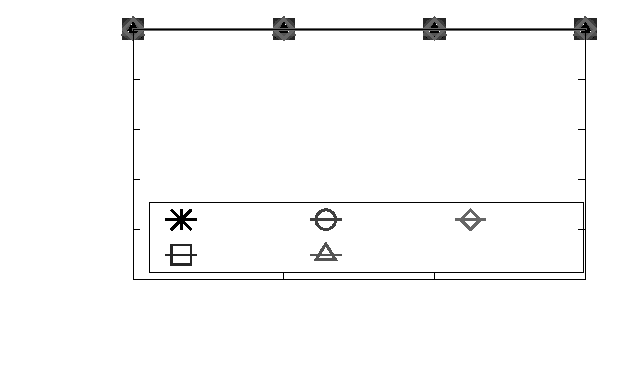
\includegraphics{normalflushreload}}%
    \gplfronttext
  \end{picture}%
\endgroup
}
\caption{$\forall \blockIdx: \ACIFn{}(\loadVar)[\blockIdx] = 0$
  \label{fig:normalcache:jaccard:flushreload}
}
\end{subfigure}% 
\caption{\JaccardRand{\secretsSetSize} for \flushreload attacks}
\end{figure}


\iffalse
\begin{table}
\caption{Selected interference rules when \cachesetNmbr=8 with memory sharing\label{tab:s8w2:shared}.}
\scriptsize{
\begingroup
\everymath{\scriptstyle}
\footnotesize
%your equation
\begin{tabular}{m{\colR}m{\colRule}m{\colPrecision}m{\colRecall}}
\toprule
 & Interference Rule (\interferenceRule{}) & Precision & Recall \\
\midrule
$\interferenceRule{0}$&$\SecFnAlt{}(\secretVar)< 2 \wedge \SecFnAlt{}(\secretVar)\ge 1 \wedge \ACIFn{}(\loadVar)[1]< 1$&1.00&0.04\\
\if 0
$\interferenceRule{1}$&$\SecFn{}(\secretVar)[1]< 1 \wedge \SecFn{}(\secretVar)< 4 \wedge \ACIFn{}(\loadVar)[1]< 1 \wedge \ACIFn{}(\loadVar)[0]< 1$&1.00&0.04\\
$\interferenceRule{2}$&$\SecFnAlt{}(\secretVar)\ge 15 \wedge \ACIFn{}(\loadVar)[15]< 1$&1.00&0.04\\
$\interferenceRule{3}$&$\SecFnAlt{}(\secretVar)\ge 13 \wedge \SecFnAlt{}(\secretVar)[1]\ge 1 \wedge \SecFnAlt{}(\secretVar)[0]\ge 1 \wedge \ACIFn{}(\loadVar)[15]< 1$&1.00&0.04\\
$\interferenceRule{4}$&$\SecFn{}(\secretVar)\ge 12 \wedge \SecFn{}(\secretVar)[1]< 1 \wedge \ACIFn{}(\loadVar)[13]< 1 \wedge \ACIFn{}(\loadVar)[12]< 1$&1.00&0.04\\
$\interferenceRule{5}$&$\SecFn{}(\secretVar)[2]\ge 1 \wedge \SecFn{}(\secretVar)[1]\ge 1 \wedge \SecFn{}(\secretVar)< 7 \wedge \ACIFn{}(\loadVar)[6]< 1$&1.00&0.04\\
$\interferenceRule{6}$&$\SecFn{}(\secretVar)\ge 11 \wedge \SecFn{}(\secretVar)[2]\ge 1 \wedge \SecFn{}(\secretVar)< 13 \wedge \ACIFn{}(\loadVar)[12]< 1$&1.00&0.04\\
$\interferenceRule{7}$&$\SecFnAlt{}(\secretVar)\ge 5 \wedge \SecFnAlt{}(\secretVar)< 7 \wedge \ACIFn{}(\loadVar)[6]< 1 \wedge \ACIFn{}(\loadVar)[5]< 1$&1.00&0.04\\
$\interferenceRule{8}$&$\SecFn{}(\secretVar)\ge 10 \wedge \SecFn{}(\secretVar)[1]< 1 \wedge \SecFn{}(\secretVar)[0]\ge 1 \wedge \ACIFn{}(\loadVar)[13]< 1$&1.00&0.04\\
$\interferenceRule{9}$&$\SecFn{}(\secretVar)[3]\ge 1 \wedge \SecFn{}(\secretVar)[2]\ge 1 \wedge \SecFn{}(\secretVar)[1]< 1 \wedge \SecFn{}(\secretVar)[0]\ge 1 \wedge \ACIFn{}(\loadVar)[13]< 1$&1.00&0.04\\
$\interferenceRule{10}$&$\SecFnAlt{}(\secretVar)\ge 4 \wedge
\SecFnAlt{}(\secretVar)[3]< 1 \wedge
\SecFnAlt{}(\secretVar)[1]\ge 1 \wedge
\SecFnAlt{}(\secretVar)[0]< 1 \wedge \ACIFn{}(\loadVar)[6]<
1$&1.00&0.04\\
\fi
\bottomrule
\end{tabular}
\endgroup
}
\end{table} 
\fi

To evaluate the leakage with memory sharing enabled (i.e., with
\Flush+\Reload attacks), we allow the attacker to control and observe
all memory blocks used by the victim by setting the base to
\texttt{0x2000000} in \proc instead of to \texttt{0x2000010} (see
\eqnref{eqn:proc}).  \figref{fig:normalcache:jaccard:sharedsymloads}
shows the corresponding \JaccardRand{\secretsSetSize}.  The
\JaccardRand{\secretsSetSize} curves are similar and close to 1 for
all settings, indicating that the leakage does not have much
correlation with \cacheLineNmbr.  An example rule for interference
derived using the methodology of \secref{dinome:sec:interpret}, having a
precision of $1.0$ and recall of $\approx 0.04$, is
\begin{align}
  \SecFnAlt{}(\secretVar)< 2 \wedge \SecFnAlt{}(\secretVar)\ge 1 \wedge \ACIFn{}(\loadVar)[1]< 1
  \label{eqn:flush-reload-interference}
\end{align}
That is, if $\SecFnAlt{}(\secretVar)=1$ then $\ACIFn{}(\loadVar)[1]=0$
results in interference.  Indeed, the other top-ranked rules for this
example (not shown) were roughly 32 similar rules, each one setting
$\ACIFn{}(\loadVar)[\blockIdx]=0$ for a specific secret value
$\SecFn{}(\secretVar)=\blockIdx$ or
$\SecFnAlt{}(\secretVar)=\blockIdx$.  The intuition behind these rules
is that an attacker can precisely detect if $\SecFn{}(\secretVar) =
\blockIdx$ by setting $\ACIFn{}(\loadVar)[\blockIdx]=0$ (i.e.,
\Flush{}ing \block{\blockIdx} so he can later \Reload it), and
similarly for $\SecFnAlt{}(\secretVar)$.  Going further, if an
attacker sets $\ACIFn{}(\loadVar)[\blockIdx] = 0$ for all \blockIdx,
he can detect the victim's access to any \block{\blockIdx}, as shown
in \figref{fig:normalcache:jaccard:flushreload} where
$\JaccardRand{\secretsSetSize}=1$ for all \secretsSetSize.

\if0
\subsubsection{Partially shared memory}
\zz{Add it \figref{fig:normal:jaccard:partial} here or not? 8-bit
\SecFn{}(\secretVar) in \proc and \texttt{base=0x2000000}. Then 16/256
memory blocks are shared and 240/256 is unshared.} The interesting
question reflected by this evaluation is when \primeprobe or
\flushreload is the best strategy when the memory is partially
shared. In \figref{fig:normal:jaccard:partial}, we present the
\JaccardRand{\secretsSetSize} when we symbolized the
\ACIFn{}(\loadVar) (denoted by `sym') or applied \primeprobe and
\flushreload. Without a specific attack strategy,
\JaccardRand{\secretsSetSize} is relatively high when
\secretsSetSize is either small enough or large enough. This indicate
that most secret value would be slightly leaked with high chance while
only a portion of secret value would be highly leaked. Under
\primeprobe attack among all cache sets, the
\JaccardRand{\secretsSetSize} decreases with the \secretsSetSize,
indicating that only a limited amount of information about the secret
could be leaked. Under \flushreload attacks among all shared blocks,
\JaccardRand{\secretsSetSize} increases with the \secretsSetSize,
indicating that a secret value would be fully leaked under a limited
chance $\leakChance = 16/256 =\approx$ 0.06 where $\JaccardRand{1} = (1-
(1-\leakChance)^2)\approx 0.12$.
\begin{figure}
\resizebox{\linewidth}{!}{\protect\footnotesize% GNUPLOT: LaTeX picture with Postscript
\begingroup
  \fontfamily{Times-Roman}%
  \selectfont
  \makeatletter
  \providecommand\color[2][]{%
    \GenericError{(gnuplot) \space\space\space\@spaces}{%
      Package color not loaded in conjunction with
      terminal option `colourtext'%
    }{See the gnuplot documentation for explanation.%
    }{Either use 'blacktext' in gnuplot or load the package
      color.sty in LaTeX.}%
    \renewcommand\color[2][]{}%
  }%
  \providecommand\includegraphics[2][]{%
    \GenericError{(gnuplot) \space\space\space\@spaces}{%
      Package graphicx or graphics not loaded%
    }{See the gnuplot documentation for explanation.%
    }{The gnuplot epslatex terminal needs graphicx.sty or graphics.sty.}%
    \renewcommand\includegraphics[2][]{}%
  }%
  \providecommand\rotatebox[2]{#2}%
  \@ifundefined{ifGPcolor}{%
    \newif\ifGPcolor
    \GPcolortrue
  }{}%
  \@ifundefined{ifGPblacktext}{%
    \newif\ifGPblacktext
    \GPblacktexttrue
  }{}%
  % define a \g@addto@macro without @ in the name:
  \let\gplgaddtomacro\g@addto@macro
  % define empty templates for all commands taking text:
  \gdef\gplbacktext{}%
  \gdef\gplfronttext{}%
  \makeatother
  \ifGPblacktext
    % no textcolor at all
    \def\colorrgb#1{}%
    \def\colorgray#1{}%
  \else
    % gray or color?
    \ifGPcolor
      \def\colorrgb#1{\color[rgb]{#1}}%
      \def\colorgray#1{\color[gray]{#1}}%
      \expandafter\def\csname LTw\endcsname{\color{white}}%
      \expandafter\def\csname LTb\endcsname{\color{black}}%
      \expandafter\def\csname LTa\endcsname{\color{black}}%
      \expandafter\def\csname LT0\endcsname{\color[rgb]{1,0,0}}%
      \expandafter\def\csname LT1\endcsname{\color[rgb]{0,1,0}}%
      \expandafter\def\csname LT2\endcsname{\color[rgb]{0,0,1}}%
      \expandafter\def\csname LT3\endcsname{\color[rgb]{1,0,1}}%
      \expandafter\def\csname LT4\endcsname{\color[rgb]{0,1,1}}%
      \expandafter\def\csname LT5\endcsname{\color[rgb]{1,1,0}}%
      \expandafter\def\csname LT6\endcsname{\color[rgb]{0,0,0}}%
      \expandafter\def\csname LT7\endcsname{\color[rgb]{1,0.3,0}}%
      \expandafter\def\csname LT8\endcsname{\color[rgb]{0.5,0.5,0.5}}%
    \else
      % gray
      \def\colorrgb#1{\color{black}}%
      \def\colorgray#1{\color[gray]{#1}}%
      \expandafter\def\csname LTw\endcsname{\color{white}}%
      \expandafter\def\csname LTb\endcsname{\color{black}}%
      \expandafter\def\csname LTa\endcsname{\color{black}}%
      \expandafter\def\csname LT0\endcsname{\color{black}}%
      \expandafter\def\csname LT1\endcsname{\color{black}}%
      \expandafter\def\csname LT2\endcsname{\color{black}}%
      \expandafter\def\csname LT3\endcsname{\color{black}}%
      \expandafter\def\csname LT4\endcsname{\color{black}}%
      \expandafter\def\csname LT5\endcsname{\color{black}}%
      \expandafter\def\csname LT6\endcsname{\color{black}}%
      \expandafter\def\csname LT7\endcsname{\color{black}}%
      \expandafter\def\csname LT8\endcsname{\color{black}}%
    \fi
  \fi
    \setlength{\unitlength}{0.0500bp}%
    \ifx\gptboxheight\undefined%
      \newlength{\gptboxheight}%
      \newlength{\gptboxwidth}%
      \newsavebox{\gptboxtext}%
    \fi%
    \setlength{\fboxrule}{0.5pt}%
    \setlength{\fboxsep}{1pt}%
\begin{picture}(5040.00,3600.00)%
    \gplgaddtomacro\gplbacktext{%
      \csname LTb\endcsname%%
      \put(962,780){\makebox(0,0)[r]{\strut{}$0$}}%
      \put(962,1318){\makebox(0,0)[r]{\strut{}$0.2$}}%
      \put(962,1856){\makebox(0,0)[r]{\strut{}$0.4$}}%
      \put(962,2393){\makebox(0,0)[r]{\strut{}$0.6$}}%
      \put(962,2931){\makebox(0,0)[r]{\strut{}$0.8$}}%
      \put(962,3469){\makebox(0,0)[r]{\strut{}$1$}}%
      \put(1118,520){\makebox(0,0){\strut{}$0$}}%
      \put(1746,520){\makebox(0,0){\strut{}$1$}}%
      \put(2373,520){\makebox(0,0){\strut{}$2$}}%
      \put(3001,520){\makebox(0,0){\strut{}$3$}}%
      \put(3628,520){\makebox(0,0){\strut{}$4$}}%
      \put(4256,520){\makebox(0,0){\strut{}$5$}}%
      \put(4883,520){\makebox(0,0){\strut{}$6$}}%
    }%
    \gplgaddtomacro\gplfronttext{%
      \csname LTb\endcsname%%
      \put(309,2124){\rotatebox{-270}{\makebox(0,0){\strut{}\JaccardRand{\secretsSetSize}}}}%
      \put(3000,182){\makebox(0,0){\strut{}$\log_2{\secretsSetSize}$}}%
      \csname LTb\endcsname%%
      \put(1805,3381){\makebox(0,0)[l]{\strut{}sym}}%
      \csname LTb\endcsname%%
      \put(1805,3069){\makebox(0,0)[l]{\strut{}primeprobe}}%
      \csname LTb\endcsname%%
      \put(1805,2757){\makebox(0,0)[l]{\strut{}flushreload}}%
    }%
    \gplbacktext
    \put(0,0){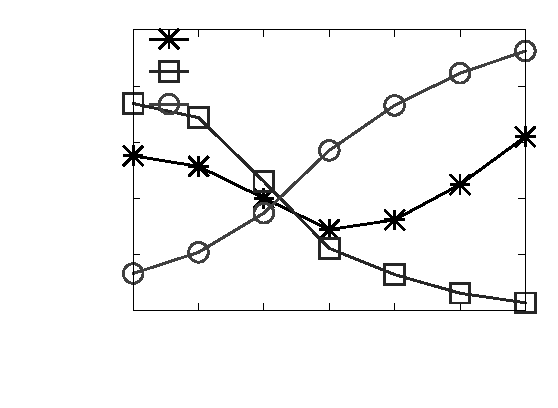
\includegraphics{normal8bit_partialshared}}%
    \gplfronttext
  \end{picture}%
\endgroup
}
\caption{8-bit secret + partially shared memory with symbolized \ACIFn{}(\loadVar)}
\label{fig:normal:jaccard:partial}
\end{figure}
\fi

\subsection{Side-channel-resistant cache designs}
\label{dinome:sec:exp:cachedefense}
\begin{figure*}
\centering
\minipage{0.49\textwidth}
%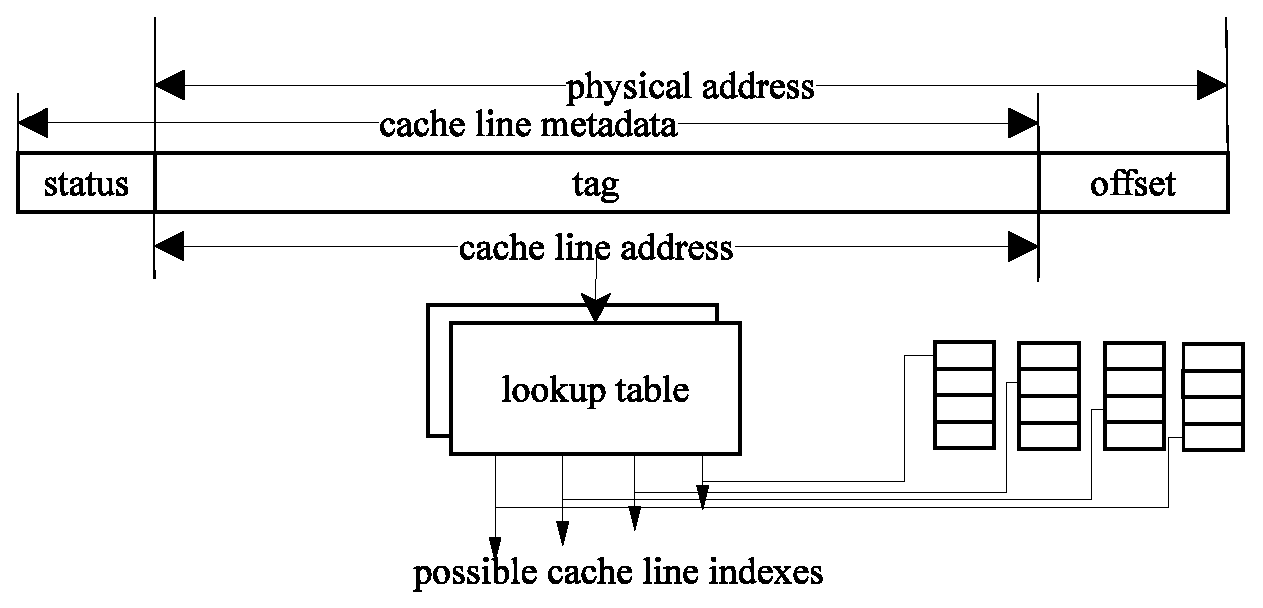
\includegraphics[width=\linewidth]{fig/dinome/scatter_tagarray.eps}
\resizebox{0.95\linewidth}{!}{\protect\footnotesize% Graphic for TeX using PGF
% Title: /Users/ziqiaozhou/zzdiss/paper/fig/scatter_tagarray_new.dia
% Creator: Dia v0.97.2
% CreationDate: Thu Jun 18 03:05:47 2020
% For: ziqiao
% \usepackage{tikz}
% The following commands are not supported in PSTricks at present
% We define them conditionally, so when they are implemented,
% this pgf file will use them.
\ifx\du\undefined
  \newlength{\du}
\fi
\setlength{\du}{15\unitlength}
\begin{tikzpicture}
\pgftransformxscale{1.000000}
\pgftransformyscale{-1.000000}
\definecolor{dialinecolor}{rgb}{0.000000, 0.000000, 0.000000}
\pgfsetstrokecolor{dialinecolor}
\definecolor{dialinecolor}{rgb}{1.000000, 1.000000, 1.000000}
\pgfsetfillcolor{dialinecolor}
\pgfsetlinewidth{0.030000\du}
\pgfsetdash{}{0pt}
\pgfsetdash{}{0pt}
\pgfsetmiterjoin
\definecolor{dialinecolor}{rgb}{1.000000, 1.000000, 1.000000}
\pgfsetfillcolor{dialinecolor}
\fill (14.953400\du,7.517166\du)--(14.953400\du,8.517166\du)--(17.286231\du,8.517166\du)--(17.286231\du,7.517166\du)--cycle;
\definecolor{dialinecolor}{rgb}{0.000000, 0.000000, 0.000000}
\pgfsetstrokecolor{dialinecolor}
\draw (14.953400\du,7.517166\du)--(14.953400\du,8.517166\du)--(17.286231\du,8.517166\du)--(17.286231\du,7.517166\du)--cycle;
\pgfsetlinewidth{0.030000\du}
\pgfsetdash{}{0pt}
\pgfsetdash{}{0pt}
\pgfsetmiterjoin
\definecolor{dialinecolor}{rgb}{1.000000, 1.000000, 1.000000}
\pgfsetfillcolor{dialinecolor}
\fill (13.315500\du,7.518066\du)--(13.315500\du,8.510834\du)--(14.950876\du,8.510834\du)--(14.950876\du,7.518066\du)--cycle;
\definecolor{dialinecolor}{rgb}{0.000000, 0.000000, 0.000000}
\pgfsetstrokecolor{dialinecolor}
\draw (13.315500\du,7.518066\du)--(13.315500\du,8.510834\du)--(14.950876\du,8.510834\du)--(14.950876\du,7.518066\du)--cycle;
\pgfsetlinewidth{0.030000\du}
\pgfsetdash{}{0pt}
\pgfsetdash{}{0pt}
\pgfsetmiterjoin
\definecolor{dialinecolor}{rgb}{1.000000, 1.000000, 1.000000}
\pgfsetfillcolor{dialinecolor}
\fill (11.615900\du,7.518066\du)--(11.615900\du,8.510834\du)--(13.308313\du,8.510834\du)--(13.308313\du,7.518066\du)--cycle;
\definecolor{dialinecolor}{rgb}{0.000000, 0.000000, 0.000000}
\pgfsetstrokecolor{dialinecolor}
\draw (11.615900\du,7.518066\du)--(11.615900\du,8.510834\du)--(13.308313\du,8.510834\du)--(13.308313\du,7.518066\du)--cycle;
\pgfsetlinewidth{0.100000\du}
\pgfsetdash{{\pgflinewidth}{0.200000\du}}{0cm}
\pgfsetdash{{\pgflinewidth}{0.200000\du}}{0cm}
\pgfsetmiterjoin
\definecolor{dialinecolor}{rgb}{1.000000, 1.000000, 1.000000}
\pgfsetfillcolor{dialinecolor}
\fill (14.954200\du,8.520716\du)--(14.954200\du,9.520716\du)--(17.286265\du,9.520716\du)--(17.286265\du,8.520716\du)--cycle;
\definecolor{dialinecolor}{rgb}{0.000000, 0.000000, 0.000000}
\pgfsetstrokecolor{dialinecolor}
\draw (14.954200\du,8.520716\du)--(14.954200\du,9.520716\du)--(17.286265\du,9.520716\du)--(17.286265\du,8.520716\du)--cycle;
\pgfsetlinewidth{0.100000\du}
\pgfsetdash{{\pgflinewidth}{0.200000\du}}{0cm}
\pgfsetdash{{\pgflinewidth}{0.200000\du}}{0cm}
\pgfsetmiterjoin
\definecolor{dialinecolor}{rgb}{1.000000, 1.000000, 1.000000}
\pgfsetfillcolor{dialinecolor}
\fill (13.307300\du,8.513076\du)--(13.307300\du,9.505844\du)--(14.942676\du,9.505844\du)--(14.942676\du,8.513076\du)--cycle;
\definecolor{dialinecolor}{rgb}{0.000000, 0.000000, 0.000000}
\pgfsetstrokecolor{dialinecolor}
\draw (13.307300\du,8.513076\du)--(13.307300\du,9.505844\du)--(14.942676\du,9.505844\du)--(14.942676\du,8.513076\du)--cycle;
\pgfsetlinewidth{0.100000\du}
\pgfsetdash{{\pgflinewidth}{0.200000\du}}{0cm}
\pgfsetdash{{\pgflinewidth}{0.200000\du}}{0cm}
\pgfsetmiterjoin
\definecolor{dialinecolor}{rgb}{1.000000, 1.000000, 1.000000}
\pgfsetfillcolor{dialinecolor}
\fill (11.607700\du,8.513076\du)--(11.607700\du,9.505844\du)--(13.300113\du,9.505844\du)--(13.300113\du,8.513076\du)--cycle;
\definecolor{dialinecolor}{rgb}{0.000000, 0.000000, 0.000000}
\pgfsetstrokecolor{dialinecolor}
\draw (11.607700\du,8.513076\du)--(11.607700\du,9.505844\du)--(13.300113\du,9.505844\du)--(13.300113\du,8.513076\du)--cycle;
\pgfsetlinewidth{0.030000\du}
\pgfsetdash{}{0pt}
\pgfsetdash{}{0pt}
\pgfsetmiterjoin
\definecolor{dialinecolor}{rgb}{1.000000, 1.000000, 1.000000}
\pgfsetfillcolor{dialinecolor}
\fill (15.360200\du,6.904006\du)--(15.360200\du,7.904006\du)--(17.693031\du,7.904006\du)--(17.693031\du,6.904006\du)--cycle;
\definecolor{dialinecolor}{rgb}{0.000000, 0.000000, 0.000000}
\pgfsetstrokecolor{dialinecolor}
\draw (15.360200\du,6.904006\du)--(15.360200\du,7.904006\du)--(17.693031\du,7.904006\du)--(17.693031\du,6.904006\du)--cycle;
\pgfsetlinewidth{0.030000\du}
\pgfsetdash{}{0pt}
\pgfsetdash{}{0pt}
\pgfsetmiterjoin
\definecolor{dialinecolor}{rgb}{1.000000, 1.000000, 1.000000}
\pgfsetfillcolor{dialinecolor}
\fill (15.360900\du,7.890906\du)--(15.360900\du,8.890906\du)--(17.692965\du,8.890906\du)--(17.692965\du,7.890906\du)--cycle;
\definecolor{dialinecolor}{rgb}{0.000000, 0.000000, 0.000000}
\pgfsetstrokecolor{dialinecolor}
\draw (15.360900\du,7.890906\du)--(15.360900\du,8.890906\du)--(17.692965\du,8.890906\du)--(17.692965\du,7.890906\du)--cycle;
\pgfsetlinewidth{0.030000\du}
\pgfsetdash{}{0pt}
\pgfsetdash{}{0pt}
\pgfsetmiterjoin
\definecolor{dialinecolor}{rgb}{1.000000, 1.000000, 1.000000}
\pgfsetfillcolor{dialinecolor}
\fill (13.722200\du,6.904896\du)--(13.722200\du,7.897664\du)--(15.357576\du,7.897664\du)--(15.357576\du,6.904896\du)--cycle;
\definecolor{dialinecolor}{rgb}{0.000000, 0.000000, 0.000000}
\pgfsetstrokecolor{dialinecolor}
\draw (13.722200\du,6.904896\du)--(13.722200\du,7.897664\du)--(15.357576\du,7.897664\du)--(15.357576\du,6.904896\du)--cycle;
\pgfsetlinewidth{0.030000\du}
\pgfsetdash{}{0pt}
\pgfsetdash{}{0pt}
\pgfsetmiterjoin
\definecolor{dialinecolor}{rgb}{1.000000, 1.000000, 1.000000}
\pgfsetfillcolor{dialinecolor}
\fill (12.022700\du,6.904896\du)--(12.022700\du,7.897664\du)--(13.715113\du,7.897664\du)--(13.715113\du,6.904896\du)--cycle;
\definecolor{dialinecolor}{rgb}{0.000000, 0.000000, 0.000000}
\pgfsetstrokecolor{dialinecolor}
\draw (12.022700\du,6.904896\du)--(12.022700\du,7.897664\du)--(13.715113\du,7.897664\du)--(13.715113\du,6.904896\du)--cycle;
\pgfsetlinewidth{0.030000\du}
\pgfsetdash{}{0pt}
\pgfsetdash{}{0pt}
\pgfsetmiterjoin
\definecolor{dialinecolor}{rgb}{1.000000, 1.000000, 1.000000}
\pgfsetfillcolor{dialinecolor}
\fill (13.714000\du,7.899916\du)--(13.714000\du,8.892684\du)--(15.349376\du,8.892684\du)--(15.349376\du,7.899916\du)--cycle;
\definecolor{dialinecolor}{rgb}{0.000000, 0.000000, 0.000000}
\pgfsetstrokecolor{dialinecolor}
\draw (13.714000\du,7.899916\du)--(13.714000\du,8.892684\du)--(15.349376\du,8.892684\du)--(15.349376\du,7.899916\du)--cycle;
\pgfsetlinewidth{0.030000\du}
\pgfsetdash{}{0pt}
\pgfsetdash{}{0pt}
\pgfsetmiterjoin
\definecolor{dialinecolor}{rgb}{1.000000, 1.000000, 1.000000}
\pgfsetfillcolor{dialinecolor}
\fill (12.014500\du,7.899916\du)--(12.014500\du,8.892684\du)--(13.706913\du,8.892684\du)--(13.706913\du,7.899916\du)--cycle;
\definecolor{dialinecolor}{rgb}{0.000000, 0.000000, 0.000000}
\pgfsetstrokecolor{dialinecolor}
\draw (12.014500\du,7.899916\du)--(12.014500\du,8.892684\du)--(13.706913\du,8.892684\du)--(13.706913\du,7.899916\du)--cycle;
\pgfsetlinewidth{0.030000\du}
\pgfsetdash{}{0pt}
\pgfsetdash{}{0pt}
\pgfsetmiterjoin
\definecolor{dialinecolor}{rgb}{1.000000, 1.000000, 1.000000}
\pgfsetfillcolor{dialinecolor}
\fill (15.773700\du,6.261216\du)--(15.773700\du,7.261216\du)--(18.105765\du,7.261216\du)--(18.105765\du,6.261216\du)--cycle;
\definecolor{dialinecolor}{rgb}{0.000000, 0.000000, 0.000000}
\pgfsetstrokecolor{dialinecolor}
\draw (15.773700\du,6.261216\du)--(15.773700\du,7.261216\du)--(18.105765\du,7.261216\du)--(18.105765\du,6.261216\du)--cycle;
\pgfsetlinewidth{0.030000\du}
\pgfsetdash{}{0pt}
\pgfsetdash{}{0pt}
\pgfsetmiterjoin
\definecolor{dialinecolor}{rgb}{1.000000, 1.000000, 1.000000}
\pgfsetfillcolor{dialinecolor}
\fill (15.766600\du,7.223906\du)--(15.766600\du,8.223906\du)--(18.098665\du,8.223906\du)--(18.098665\du,7.223906\du)--cycle;
\definecolor{dialinecolor}{rgb}{0.000000, 0.000000, 0.000000}
\pgfsetstrokecolor{dialinecolor}
\draw (15.766600\du,7.223906\du)--(15.766600\du,8.223906\du)--(18.098665\du,8.223906\du)--(18.098665\du,7.223906\du)--cycle;
\pgfsetlinewidth{0.030000\du}
\pgfsetdash{}{0pt}
\pgfsetdash{}{0pt}
\pgfsetmiterjoin
\definecolor{dialinecolor}{rgb}{1.000000, 1.000000, 1.000000}
\pgfsetfillcolor{dialinecolor}
\fill (14.128000\du,6.255506\du)--(14.128000\du,7.248274\du)--(15.763376\du,7.248274\du)--(15.763376\du,6.255506\du)--cycle;
\definecolor{dialinecolor}{rgb}{0.000000, 0.000000, 0.000000}
\pgfsetstrokecolor{dialinecolor}
\draw (14.128000\du,6.255506\du)--(14.128000\du,7.248274\du)--(15.763376\du,7.248274\du)--(15.763376\du,6.255506\du)--cycle;
\pgfsetlinewidth{0.030000\du}
\pgfsetdash{}{0pt}
\pgfsetdash{}{0pt}
\pgfsetmiterjoin
\definecolor{dialinecolor}{rgb}{1.000000, 1.000000, 1.000000}
\pgfsetfillcolor{dialinecolor}
\fill (12.428400\du,6.255506\du)--(12.428400\du,7.248274\du)--(14.120813\du,7.248274\du)--(14.120813\du,6.255506\du)--cycle;
\definecolor{dialinecolor}{rgb}{0.000000, 0.000000, 0.000000}
\pgfsetstrokecolor{dialinecolor}
\draw (12.428400\du,6.255506\du)--(12.428400\du,7.248274\du)--(14.120813\du,7.248274\du)--(14.120813\du,6.255506\du)--cycle;
\pgfsetlinewidth{0.030000\du}
\pgfsetdash{}{0pt}
\pgfsetdash{}{0pt}
\pgfsetmiterjoin
\definecolor{dialinecolor}{rgb}{1.000000, 1.000000, 1.000000}
\pgfsetfillcolor{dialinecolor}
\fill (14.127100\du,7.226636\du)--(14.127100\du,8.219404\du)--(15.762476\du,8.219404\du)--(15.762476\du,7.226636\du)--cycle;
\definecolor{dialinecolor}{rgb}{0.000000, 0.000000, 0.000000}
\pgfsetstrokecolor{dialinecolor}
\draw (14.127100\du,7.226636\du)--(14.127100\du,8.219404\du)--(15.762476\du,8.219404\du)--(15.762476\du,7.226636\du)--cycle;
\pgfsetlinewidth{0.030000\du}
\pgfsetdash{}{0pt}
\pgfsetdash{}{0pt}
\pgfsetmiterjoin
\definecolor{dialinecolor}{rgb}{1.000000, 1.000000, 1.000000}
\pgfsetfillcolor{dialinecolor}
\fill (12.427500\du,7.226636\du)--(12.427500\du,8.219404\du)--(14.119913\du,8.219404\du)--(14.119913\du,7.226636\du)--cycle;
\definecolor{dialinecolor}{rgb}{0.000000, 0.000000, 0.000000}
\pgfsetstrokecolor{dialinecolor}
\draw (12.427500\du,7.226636\du)--(12.427500\du,8.219404\du)--(14.119913\du,8.219404\du)--(14.119913\du,7.226636\du)--cycle;
\definecolor{dialinecolor}{rgb}{1.000000, 1.000000, 1.000000}
\pgfsetfillcolor{dialinecolor}
\fill (13.576000\du,4.664585\du)--(13.576000\du,5.372085\du)--(15.886000\du,5.372085\du)--(15.886000\du,4.664585\du)--cycle;
% setfont left to latex
\definecolor{dialinecolor}{rgb}{0.000000, 0.000000, 0.000000}
\pgfsetstrokecolor{dialinecolor}
\node at (14.731000\du,5.234585\du){metadata};
\pgfsetlinewidth{0.080000\du}
\pgfsetdash{}{0pt}
\pgfsetdash{}{0pt}
\pgfsetmiterjoin
\pgfsetbuttcap
{
\definecolor{dialinecolor}{rgb}{0.000000, 0.000000, 0.000000}
\pgfsetfillcolor{dialinecolor}
% was here!!!
\pgfsetarrowsend{latex}
{\pgfsetcornersarced{\pgfpoint{0.000000\du}{0.000000\du}}\definecolor{dialinecolor}{rgb}{0.000000, 0.000000, 0.000000}
\pgfsetstrokecolor{dialinecolor}
\draw (7.651291\du,5.313240\du)--(7.651291\du,5.995305\du)--(7.654036\du,5.995305\du)--(7.654036\du,6.677370\du);
}}
\pgfsetlinewidth{0.080000\du}
\pgfsetdash{}{0pt}
\pgfsetdash{}{0pt}
\pgfsetmiterjoin
\pgfsetbuttcap
{
\definecolor{dialinecolor}{rgb}{0.000000, 0.000000, 0.000000}
\pgfsetfillcolor{dialinecolor}
% was here!!!
{\pgfsetcornersarced{\pgfpoint{0.000000\du}{0.000000\du}}\definecolor{dialinecolor}{rgb}{0.000000, 0.000000, 0.000000}
\pgfsetstrokecolor{dialinecolor}
\draw (8.868025\du,8.836026\du)--(10.625000\du,8.836026\du)--(10.625000\du,6.095930\du)--(12.827600\du,6.095930\du);
}}
% setfont left to latex
\definecolor{dialinecolor}{rgb}{0.000000, 0.000000, 0.000000}
\pgfsetstrokecolor{dialinecolor}
\node at (9.407599\du,9.793287\du){cache line indexes};
\pgfsetlinewidth{0.030000\du}
\pgfsetdash{}{0pt}
\pgfsetdash{}{0pt}
\pgfsetbuttcap
{
\definecolor{dialinecolor}{rgb}{0.000000, 0.000000, 0.000000}
\pgfsetfillcolor{dialinecolor}
% was here!!!
\pgfsetarrowsstart{latex}
\pgfsetarrowsend{latex}
\definecolor{dialinecolor}{rgb}{0.000000, 0.000000, 0.000000}
\pgfsetstrokecolor{dialinecolor}
\draw (4.731420\du,5.855600\du)--(10.577600\du,5.857115\du);
}
\definecolor{dialinecolor}{rgb}{1.000000, 1.000000, 1.000000}
\pgfsetfillcolor{dialinecolor}
\fill (5.496750\du,5.282290\du)--(5.496750\du,5.989790\du)--(10.159250\du,5.989790\du)--(10.159250\du,5.282290\du)--cycle;
% setfont left to latex
\definecolor{dialinecolor}{rgb}{0.000000, 0.000000, 0.000000}
\pgfsetstrokecolor{dialinecolor}
\node at (7.828000\du,5.852290\du){cache line address};
\pgfsetlinewidth{0.030000\du}
\pgfsetdash{}{0pt}
\pgfsetdash{}{0pt}
\pgfsetbuttcap
{
\definecolor{dialinecolor}{rgb}{0.000000, 0.000000, 0.000000}
\pgfsetfillcolor{dialinecolor}
% was here!!!
\definecolor{dialinecolor}{rgb}{0.000000, 0.000000, 0.000000}
\pgfsetstrokecolor{dialinecolor}
\draw (4.729300\du,5.313240\du)--(4.733540\du,6.397960\du);
}
\pgfsetlinewidth{0.030000\du}
\pgfsetdash{}{0pt}
\pgfsetdash{}{0pt}
\pgfsetbuttcap
{
\definecolor{dialinecolor}{rgb}{0.000000, 0.000000, 0.000000}
\pgfsetfillcolor{dialinecolor}
% was here!!!
\definecolor{dialinecolor}{rgb}{0.000000, 0.000000, 0.000000}
\pgfsetstrokecolor{dialinecolor}
\draw (10.575500\du,5.312920\du)--(10.579700\du,6.401310\du);
}
\pgfsetlinewidth{0.030000\du}
\pgfsetdash{}{0pt}
\pgfsetdash{}{0pt}
\pgfsetbuttcap
{
\definecolor{dialinecolor}{rgb}{0.000000, 0.000000, 0.000000}
\pgfsetfillcolor{dialinecolor}
% was here!!!
\definecolor{dialinecolor}{rgb}{0.000000, 0.000000, 0.000000}
\pgfsetstrokecolor{dialinecolor}
\draw (13.086300\du,3.570320\du)--(13.085100\du,4.312920\du);
}
\pgfsetlinewidth{0.030000\du}
\pgfsetdash{}{0pt}
\pgfsetdash{}{0pt}
\pgfsetbuttcap
{
\definecolor{dialinecolor}{rgb}{0.000000, 0.000000, 0.000000}
\pgfsetfillcolor{dialinecolor}
% was here!!!
\pgfsetarrowsstart{latex}
\pgfsetarrowsend{latex}
\definecolor{dialinecolor}{rgb}{0.000000, 0.000000, 0.000000}
\pgfsetstrokecolor{dialinecolor}
\draw (4.723030\du,3.887680\du)--(13.088300\du,3.890470\du);
}
\definecolor{dialinecolor}{rgb}{1.000000, 1.000000, 1.000000}
\pgfsetfillcolor{dialinecolor}
\fill (6.795665\du,3.319075\du)--(6.795665\du,4.026575\du)--(11.015665\du,4.026575\du)--(11.015665\du,3.319075\du)--cycle;
% setfont left to latex
\definecolor{dialinecolor}{rgb}{0.000000, 0.000000, 0.000000}
\pgfsetstrokecolor{dialinecolor}
\node at (8.905665\du,3.889075\du){physical address};
\pgfsetlinewidth{0.030000\du}
\pgfsetdash{}{0pt}
\pgfsetdash{}{0pt}
\pgfsetbuttcap
{
\definecolor{dialinecolor}{rgb}{0.000000, 0.000000, 0.000000}
\pgfsetfillcolor{dialinecolor}
% was here!!!
\definecolor{dialinecolor}{rgb}{0.000000, 0.000000, 0.000000}
\pgfsetstrokecolor{dialinecolor}
\draw (4.732750\du,3.578350\du)--(4.729300\du,4.313240\du);
}
\pgfsetlinewidth{0.050000\du}
\pgfsetdash{}{0pt}
\pgfsetdash{}{0pt}
\pgfsetmiterjoin
\definecolor{dialinecolor}{rgb}{1.000000, 1.000000, 1.000000}
\pgfsetfillcolor{dialinecolor}
\fill (4.729300\du,4.313240\du)--(4.729300\du,5.313240\du)--(10.573283\du,5.313240\du)--(10.573283\du,4.313240\du)--cycle;
\definecolor{dialinecolor}{rgb}{0.000000, 0.000000, 0.000000}
\pgfsetstrokecolor{dialinecolor}
\draw (4.729300\du,4.313240\du)--(4.729300\du,5.313240\du)--(10.573283\du,5.313240\du)--(10.573283\du,4.313240\du)--cycle;
% setfont left to latex
\definecolor{dialinecolor}{rgb}{0.000000, 0.000000, 0.000000}
\pgfsetstrokecolor{dialinecolor}
\node at (7.651290\du,4.813240\du){tag};
\pgfsetlinewidth{0.050000\du}
\pgfsetdash{}{0pt}
\pgfsetdash{}{0pt}
\pgfsetmiterjoin
\definecolor{dialinecolor}{rgb}{1.000000, 1.000000, 1.000000}
\pgfsetfillcolor{dialinecolor}
\fill (10.575500\du,4.312920\du)--(10.575500\du,5.312920\du)--(13.085145\du,5.312920\du)--(13.085145\du,4.312920\du)--cycle;
\definecolor{dialinecolor}{rgb}{0.000000, 0.000000, 0.000000}
\pgfsetstrokecolor{dialinecolor}
\draw (10.575500\du,4.312920\du)--(10.575500\du,5.312920\du)--(13.085145\du,5.312920\du)--(13.085145\du,4.312920\du)--cycle;
% setfont left to latex
\definecolor{dialinecolor}{rgb}{0.000000, 0.000000, 0.000000}
\pgfsetstrokecolor{dialinecolor}
\node at (11.830300\du,4.812920\du){offset};
\pgfsetlinewidth{0.030000\du}
\pgfsetdash{}{0pt}
\pgfsetdash{}{0pt}
\pgfsetmiterjoin
\definecolor{dialinecolor}{rgb}{1.000000, 1.000000, 1.000000}
\pgfsetfillcolor{dialinecolor}
\fill (14.518900\du,6.594556\du)--(14.518900\du,7.587324\du)--(16.154276\du,7.587324\du)--(16.154276\du,6.594556\du)--cycle;
\definecolor{dialinecolor}{rgb}{0.000000, 0.000000, 0.000000}
\pgfsetstrokecolor{dialinecolor}
\draw (14.518900\du,6.594556\du)--(14.518900\du,7.587324\du)--(16.154276\du,7.587324\du)--(16.154276\du,6.594556\du)--cycle;
\pgfsetlinewidth{0.030000\du}
\pgfsetdash{}{0pt}
\pgfsetdash{}{0pt}
\pgfsetmiterjoin
\definecolor{dialinecolor}{rgb}{1.000000, 1.000000, 1.000000}
\pgfsetfillcolor{dialinecolor}
\fill (12.819400\du,6.594556\du)--(12.819400\du,7.587324\du)--(14.511813\du,7.587324\du)--(14.511813\du,6.594556\du)--cycle;
\definecolor{dialinecolor}{rgb}{0.000000, 0.000000, 0.000000}
\pgfsetstrokecolor{dialinecolor}
\draw (12.819400\du,6.594556\du)--(12.819400\du,7.587324\du)--(14.511813\du,7.587324\du)--(14.511813\du,6.594556\du)--cycle;
% setfont left to latex
\definecolor{dialinecolor}{rgb}{0.000000, 0.000000, 0.000000}
\pgfsetstrokecolor{dialinecolor}
\node at (13.665606\du,7.090940\du){status};
% setfont left to latex
\definecolor{dialinecolor}{rgb}{0.000000, 0.000000, 0.000000}
\pgfsetstrokecolor{dialinecolor}
\node at (15.336588\du,7.090940\du){tag};
\pgfsetlinewidth{0.100000\du}
\pgfsetdash{{1.000000\du}{1.000000\du}}{0\du}
\pgfsetdash{{0.100000\du}{0.100000\du}}{0\du}
\pgfsetmiterjoin
\definecolor{dialinecolor}{rgb}{1.000000, 1.000000, 1.000000}
\pgfsetfillcolor{dialinecolor}
\fill (14.527100\du,5.599546\du)--(14.527100\du,6.592314\du)--(16.162476\du,6.592314\du)--(16.162476\du,5.599546\du)--cycle;
\definecolor{dialinecolor}{rgb}{0.000000, 0.000000, 0.000000}
\pgfsetstrokecolor{dialinecolor}
\draw (14.527100\du,5.599546\du)--(14.527100\du,6.592314\du)--(16.162476\du,6.592314\du)--(16.162476\du,5.599546\du)--cycle;
\pgfsetlinewidth{0.100000\du}
\pgfsetdash{{0.100000\du}{0.100000\du}}{0\du}
\pgfsetdash{{0.100000\du}{0.100000\du}}{0\du}
\pgfsetmiterjoin
\definecolor{dialinecolor}{rgb}{1.000000, 1.000000, 1.000000}
\pgfsetfillcolor{dialinecolor}
\fill (12.827600\du,5.599546\du)--(12.827600\du,6.592314\du)--(14.520013\du,6.592314\du)--(14.520013\du,5.599546\du)--cycle;
\definecolor{dialinecolor}{rgb}{0.000000, 0.000000, 0.000000}
\pgfsetstrokecolor{dialinecolor}
\draw (12.827600\du,5.599546\du)--(12.827600\du,6.592314\du)--(14.520013\du,6.592314\du)--(14.520013\du,5.599546\du)--cycle;
% setfont left to latex
\definecolor{dialinecolor}{rgb}{0.000000, 0.000000, 0.000000}
\pgfsetstrokecolor{dialinecolor}
\node at (13.673806\du,6.095930\du){status};
% setfont left to latex
\definecolor{dialinecolor}{rgb}{0.000000, 0.000000, 0.000000}
\pgfsetstrokecolor{dialinecolor}
\node at (15.344788\du,6.095930\du){tag};
\pgfsetlinewidth{0.030000\du}
\pgfsetdash{}{0pt}
\pgfsetdash{}{0pt}
\pgfsetmiterjoin
\definecolor{dialinecolor}{rgb}{1.000000, 1.000000, 1.000000}
\pgfsetfillcolor{dialinecolor}
\fill (16.143700\du,6.585556\du)--(16.143700\du,7.585556\du)--(18.475765\du,7.585556\du)--(18.475765\du,6.585556\du)--cycle;
\definecolor{dialinecolor}{rgb}{0.000000, 0.000000, 0.000000}
\pgfsetstrokecolor{dialinecolor}
\draw (16.143700\du,6.585556\du)--(16.143700\du,7.585556\du)--(18.475765\du,7.585556\du)--(18.475765\du,6.585556\du)--cycle;
\pgfsetlinewidth{0.100000\du}
\pgfsetdash{{1.000000\du}{1.000000\du}}{0\du}
\pgfsetdash{{0.100000\du}{0.100000\du}}{0\du}
\pgfsetmiterjoin
\definecolor{dialinecolor}{rgb}{1.000000, 1.000000, 1.000000}
\pgfsetfillcolor{dialinecolor}
\fill (16.165000\du,5.598646\du)--(16.165000\du,6.588899\du)--(18.466926\du,6.588899\du)--(18.466926\du,5.598646\du)--cycle;
\definecolor{dialinecolor}{rgb}{0.000000, 0.000000, 0.000000}
\pgfsetstrokecolor{dialinecolor}
\draw (16.165000\du,5.598646\du)--(16.165000\du,6.588899\du)--(18.466926\du,6.588899\du)--(18.466926\du,5.598646\du)--cycle;
\definecolor{dialinecolor}{rgb}{1.000000, 1.000000, 1.000000}
\pgfsetfillcolor{dialinecolor}
\fill (17.002250\du,4.667575\du)--(17.002250\du,5.375075\du)--(18.069750\du,5.375075\du)--(18.069750\du,4.667575\du)--cycle;
% setfont left to latex
\definecolor{dialinecolor}{rgb}{0.000000, 0.000000, 0.000000}
\pgfsetstrokecolor{dialinecolor}
\node at (17.536000\du,5.237575\du){data};
\pgfsetlinewidth{0.080000\du}
\pgfsetdash{}{0pt}
\pgfsetdash{}{0pt}
\pgfsetbuttcap
{
\definecolor{dialinecolor}{rgb}{0.000000, 0.000000, 0.000000}
\pgfsetfillcolor{dialinecolor}
% was here!!!
\pgfsetarrowsend{latex}
\definecolor{dialinecolor}{rgb}{0.000000, 0.000000, 0.000000}
\pgfsetstrokecolor{dialinecolor}
\draw (8.868570\du,8.505796\du)--(8.867480\du,9.166256\du);
}
\pgfsetlinewidth{0.080000\du}
\pgfsetdash{}{0pt}
\pgfsetdash{}{0pt}
\pgfsetbuttcap
{
\definecolor{dialinecolor}{rgb}{0.000000, 0.000000, 0.000000}
\pgfsetfillcolor{dialinecolor}
% was here!!!
\pgfsetarrowsend{latex}
\definecolor{dialinecolor}{rgb}{0.000000, 0.000000, 0.000000}
\pgfsetstrokecolor{dialinecolor}
\draw (7.085750\du,8.507996\du)--(7.090980\du,9.510936\du);
}
\pgfsetlinewidth{0.050000\du}
\pgfsetdash{}{0pt}
\pgfsetdash{}{0pt}
\pgfsetmiterjoin
\definecolor{dialinecolor}{rgb}{1.000000, 1.000000, 1.000000}
\pgfsetfillcolor{dialinecolor}
\fill (6.013821\du,6.677370\du)--(6.013821\du,8.205134\du)--(9.294250\du,8.205134\du)--(9.294250\du,6.677370\du)--cycle;
\definecolor{dialinecolor}{rgb}{0.000000, 0.000000, 0.000000}
\pgfsetstrokecolor{dialinecolor}
\draw (6.013821\du,6.677370\du)--(6.013821\du,8.205134\du)--(9.294250\du,8.205134\du)--(9.294250\du,6.677370\du)--cycle;
\pgfsetlinewidth{0.050000\du}
\pgfsetdash{}{0pt}
\pgfsetdash{}{0pt}
\pgfsetmiterjoin
\definecolor{dialinecolor}{rgb}{1.000000, 1.000000, 1.000000}
\pgfsetfillcolor{dialinecolor}
\fill (6.300070\du,6.924497\du)--(6.300070\du,8.493756\du)--(9.580499\du,8.493756\du)--(9.580499\du,6.924497\du)--cycle;
\definecolor{dialinecolor}{rgb}{0.000000, 0.000000, 0.000000}
\pgfsetstrokecolor{dialinecolor}
\draw (6.300070\du,6.924497\du)--(6.300070\du,8.493756\du)--(9.580499\du,8.493756\du)--(9.580499\du,6.924497\du)--cycle;
% setfont left to latex
\definecolor{dialinecolor}{rgb}{0.000000, 0.000000, 0.000000}
\pgfsetstrokecolor{dialinecolor}
\node at (7.940284\du,7.709126\du){\ensuremath{\cacheMap{0}}};
\pgfsetlinewidth{0.080000\du}
\pgfsetdash{}{0pt}
\pgfsetdash{}{0pt}
\pgfsetbuttcap
{
\definecolor{dialinecolor}{rgb}{0.000000, 0.000000, 0.000000}
\pgfsetfillcolor{dialinecolor}
% was here!!!
\definecolor{dialinecolor}{rgb}{0.000000, 0.000000, 0.000000}
\pgfsetstrokecolor{dialinecolor}
\draw (7.088365\du,9.009466\du)--(11.607700\du,9.009460\du);
}
\end{tikzpicture}
}
\caption{\scatterCache \label{fig:scatterTagarray}}
\endminipage
\centering
\minipage{0.49\textwidth}
%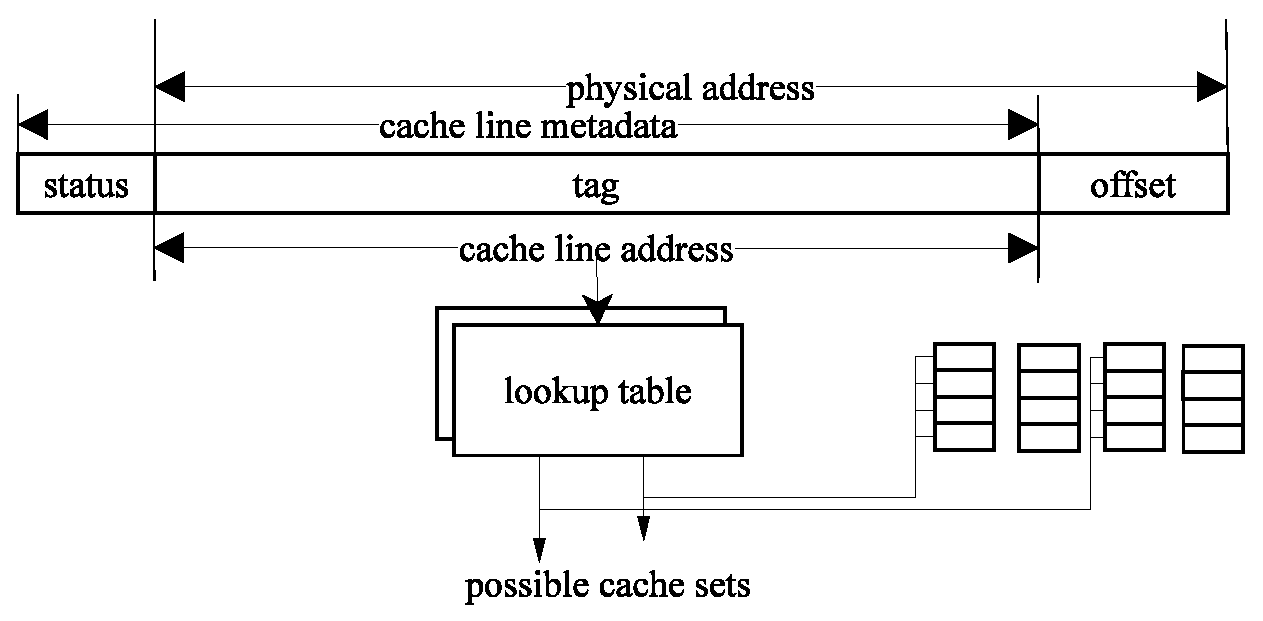
\includegraphics[width=\linewidth]{fig/dinome/phantom_tagarray.eps}
\resizebox{0.95\linewidth}{!}{\protect\footnotesize% Graphic for TeX using PGF
% Title: /Users/ziqiaozhou/zzdiss/paper/fig/phantom_tagarray_new.dia
% Creator: Dia v0.97.2
% CreationDate: Thu Jun 18 03:05:32 2020
% For: ziqiao
% \usepackage{tikz}
% The following commands are not supported in PSTricks at present
% We define them conditionally, so when they are implemented,
% this pgf file will use them.
\ifx\du\undefined
  \newlength{\du}
\fi
\setlength{\du}{15\unitlength}
\begin{tikzpicture}
\pgftransformxscale{1.000000}
\pgftransformyscale{-1.000000}
\definecolor{dialinecolor}{rgb}{0.000000, 0.000000, 0.000000}
\pgfsetstrokecolor{dialinecolor}
\definecolor{dialinecolor}{rgb}{1.000000, 1.000000, 1.000000}
\pgfsetfillcolor{dialinecolor}
\pgfsetlinewidth{0.100000\du}
\pgfsetdash{{1.000000\du}{1.000000\du}}{0\du}
\pgfsetdash{{0.100000\du}{0.100000\du}}{0\du}
\pgfsetmiterjoin
\definecolor{dialinecolor}{rgb}{1.000000, 1.000000, 1.000000}
\pgfsetfillcolor{dialinecolor}
\fill (13.751400\du,8.540526\du)--(13.751400\du,9.533293\du)--(15.386776\du,9.533293\du)--(15.386776\du,8.540526\du)--cycle;
\definecolor{dialinecolor}{rgb}{0.000000, 0.000000, 0.000000}
\pgfsetstrokecolor{dialinecolor}
\draw (13.751400\du,8.540526\du)--(13.751400\du,9.533293\du)--(15.386776\du,9.533293\du)--(15.386776\du,8.540526\du)--cycle;
\pgfsetlinewidth{0.100000\du}
\pgfsetdash{{0.100000\du}{0.100000\du}}{0\du}
\pgfsetdash{{0.100000\du}{0.100000\du}}{0\du}
\pgfsetmiterjoin
\definecolor{dialinecolor}{rgb}{1.000000, 1.000000, 1.000000}
\pgfsetfillcolor{dialinecolor}
\fill (13.759600\du,7.545516\du)--(13.759600\du,8.538283\du)--(15.394976\du,8.538283\du)--(15.394976\du,7.545516\du)--cycle;
\definecolor{dialinecolor}{rgb}{0.000000, 0.000000, 0.000000}
\pgfsetstrokecolor{dialinecolor}
\draw (13.759600\du,7.545516\du)--(13.759600\du,8.538283\du)--(15.394976\du,8.538283\du)--(15.394976\du,7.545516\du)--cycle;
\pgfsetlinewidth{0.100000\du}
\pgfsetdash{{0.100000\du}{0.100000\du}}{0\du}
\pgfsetdash{{0.100000\du}{0.100000\du}}{0\du}
\pgfsetmiterjoin
\definecolor{dialinecolor}{rgb}{1.000000, 1.000000, 1.000000}
\pgfsetfillcolor{dialinecolor}
\fill (12.060100\du,7.545516\du)--(12.060100\du,8.538283\du)--(13.803126\du,8.538283\du)--(13.803126\du,7.545516\du)--cycle;
\definecolor{dialinecolor}{rgb}{0.000000, 0.000000, 0.000000}
\pgfsetstrokecolor{dialinecolor}
\draw (12.060100\du,7.545516\du)--(12.060100\du,8.538283\du)--(13.803126\du,8.538283\du)--(13.803126\du,7.545516\du)--cycle;
\pgfsetlinewidth{0.100000\du}
\pgfsetdash{{0.100000\du}{0.100000\du}}{0\du}
\pgfsetdash{{0.100000\du}{0.100000\du}}{0\du}
\pgfsetmiterjoin
\definecolor{dialinecolor}{rgb}{1.000000, 1.000000, 1.000000}
\pgfsetfillcolor{dialinecolor}
\fill (15.376200\du,8.531526\du)--(15.376200\du,9.531526\du)--(17.708265\du,9.531526\du)--(17.708265\du,8.531526\du)--cycle;
\definecolor{dialinecolor}{rgb}{0.000000, 0.000000, 0.000000}
\pgfsetstrokecolor{dialinecolor}
\draw (15.376200\du,8.531526\du)--(15.376200\du,9.531526\du)--(17.708265\du,9.531526\du)--(17.708265\du,8.531526\du)--cycle;
\pgfsetlinewidth{0.100000\du}
\pgfsetdash{{0.100000\du}{0.100000\du}}{0\du}
\pgfsetdash{{0.100000\du}{0.100000\du}}{0\du}
\pgfsetmiterjoin
\definecolor{dialinecolor}{rgb}{1.000000, 1.000000, 1.000000}
\pgfsetfillcolor{dialinecolor}
\fill (15.397600\du,7.544616\du)--(15.397600\du,8.534869\du)--(17.730431\du,8.534869\du)--(17.730431\du,7.544616\du)--cycle;
\definecolor{dialinecolor}{rgb}{0.000000, 0.000000, 0.000000}
\pgfsetstrokecolor{dialinecolor}
\draw (15.397600\du,7.544616\du)--(15.397600\du,8.534869\du)--(17.730431\du,8.534869\du)--(17.730431\du,7.544616\du)--cycle;
\pgfsetlinewidth{0.100000\du}
\pgfsetdash{{0.100000\du}{0.100000\du}}{0\du}
\pgfsetdash{{0.100000\du}{0.100000\du}}{0\du}
\pgfsetmiterjoin
\definecolor{dialinecolor}{rgb}{1.000000, 1.000000, 1.000000}
\pgfsetfillcolor{dialinecolor}
\fill (12.048300\du,8.528306\du)--(12.048300\du,9.521073\du)--(13.791326\du,9.521073\du)--(13.791326\du,8.528306\du)--cycle;
\definecolor{dialinecolor}{rgb}{0.000000, 0.000000, 0.000000}
\pgfsetstrokecolor{dialinecolor}
\draw (12.048300\du,8.528306\du)--(12.048300\du,9.521073\du)--(13.791326\du,9.521073\du)--(13.791326\du,8.528306\du)--cycle;
\pgfsetlinewidth{0.030000\du}
\pgfsetdash{}{0pt}
\pgfsetdash{}{0pt}
\pgfsetmiterjoin
\definecolor{dialinecolor}{rgb}{1.000000, 1.000000, 1.000000}
\pgfsetfillcolor{dialinecolor}
\fill (14.118400\du,7.888695\du)--(14.118400\du,8.881463\du)--(15.753776\du,8.881463\du)--(15.753776\du,7.888695\du)--cycle;
\definecolor{dialinecolor}{rgb}{0.000000, 0.000000, 0.000000}
\pgfsetstrokecolor{dialinecolor}
\draw (14.118400\du,7.888695\du)--(14.118400\du,8.881463\du)--(15.753776\du,8.881463\du)--(15.753776\du,7.888695\du)--cycle;
\pgfsetlinewidth{0.030000\du}
\pgfsetdash{}{0pt}
\pgfsetdash{}{0pt}
\pgfsetmiterjoin
\definecolor{dialinecolor}{rgb}{1.000000, 1.000000, 1.000000}
\pgfsetfillcolor{dialinecolor}
\fill (12.418800\du,7.888695\du)--(12.418800\du,8.881463\du)--(14.111213\du,8.881463\du)--(14.111213\du,7.888695\du)--cycle;
\definecolor{dialinecolor}{rgb}{0.000000, 0.000000, 0.000000}
\pgfsetstrokecolor{dialinecolor}
\draw (12.418800\du,7.888695\du)--(12.418800\du,8.881463\du)--(14.111213\du,8.881463\du)--(14.111213\du,7.888695\du)--cycle;
\pgfsetlinewidth{0.030000\du}
\pgfsetdash{}{0pt}
\pgfsetdash{}{0pt}
\pgfsetmiterjoin
\definecolor{dialinecolor}{rgb}{1.000000, 1.000000, 1.000000}
\pgfsetfillcolor{dialinecolor}
\fill (14.126600\du,6.893685\du)--(14.126600\du,7.886453\du)--(15.761976\du,7.886453\du)--(15.761976\du,6.893685\du)--cycle;
\definecolor{dialinecolor}{rgb}{0.000000, 0.000000, 0.000000}
\pgfsetstrokecolor{dialinecolor}
\draw (14.126600\du,6.893685\du)--(14.126600\du,7.886453\du)--(15.761976\du,7.886453\du)--(15.761976\du,6.893685\du)--cycle;
\pgfsetlinewidth{0.030000\du}
\pgfsetdash{}{0pt}
\pgfsetdash{}{0pt}
\pgfsetmiterjoin
\definecolor{dialinecolor}{rgb}{1.000000, 1.000000, 1.000000}
\pgfsetfillcolor{dialinecolor}
\fill (12.427000\du,6.893685\du)--(12.427000\du,7.886453\du)--(14.119413\du,7.886453\du)--(14.119413\du,6.893685\du)--cycle;
\definecolor{dialinecolor}{rgb}{0.000000, 0.000000, 0.000000}
\pgfsetstrokecolor{dialinecolor}
\draw (12.427000\du,6.893685\du)--(12.427000\du,7.886453\du)--(14.119413\du,7.886453\du)--(14.119413\du,6.893685\du)--cycle;
\pgfsetlinewidth{0.030000\du}
\pgfsetdash{}{0pt}
\pgfsetdash{}{0pt}
\pgfsetmiterjoin
\definecolor{dialinecolor}{rgb}{1.000000, 1.000000, 1.000000}
\pgfsetfillcolor{dialinecolor}
\fill (15.743100\du,7.879695\du)--(15.743100\du,8.879695\du)--(18.075165\du,8.879695\du)--(18.075165\du,7.879695\du)--cycle;
\definecolor{dialinecolor}{rgb}{0.000000, 0.000000, 0.000000}
\pgfsetstrokecolor{dialinecolor}
\draw (15.743100\du,7.879695\du)--(15.743100\du,8.879695\du)--(18.075165\du,8.879695\du)--(18.075165\du,7.879695\du)--cycle;
\pgfsetlinewidth{0.030000\du}
\pgfsetdash{}{0pt}
\pgfsetdash{}{0pt}
\pgfsetmiterjoin
\definecolor{dialinecolor}{rgb}{1.000000, 1.000000, 1.000000}
\pgfsetfillcolor{dialinecolor}
\fill (15.764500\du,6.892785\du)--(15.764500\du,7.883038\du)--(18.097331\du,7.883038\du)--(18.097331\du,6.892785\du)--cycle;
\definecolor{dialinecolor}{rgb}{0.000000, 0.000000, 0.000000}
\pgfsetstrokecolor{dialinecolor}
\draw (15.764500\du,6.892785\du)--(15.764500\du,7.883038\du)--(18.097331\du,7.883038\du)--(18.097331\du,6.892785\du)--cycle;
\pgfsetlinewidth{0.050000\du}
\pgfsetdash{}{0pt}
\pgfsetdash{}{0pt}
\pgfsetmiterjoin
\definecolor{dialinecolor}{rgb}{1.000000, 1.000000, 1.000000}
\pgfsetfillcolor{dialinecolor}
\fill (6.379780\du,6.658681\du)--(6.379780\du,8.243927\du)--(9.660209\du,8.243927\du)--(9.660209\du,6.658681\du)--cycle;
\definecolor{dialinecolor}{rgb}{0.000000, 0.000000, 0.000000}
\pgfsetstrokecolor{dialinecolor}
\draw (6.379780\du,6.658681\du)--(6.379780\du,8.243927\du)--(9.660209\du,8.243927\du)--(9.660209\du,6.658681\du)--cycle;
\pgfsetlinewidth{0.080000\du}
\pgfsetdash{}{0pt}
\pgfsetdash{}{0pt}
\pgfsetmiterjoin
\pgfsetbuttcap
{
\definecolor{dialinecolor}{rgb}{0.000000, 0.000000, 0.000000}
\pgfsetfillcolor{dialinecolor}
% was here!!!
\pgfsetarrowsend{latex}
{\pgfsetcornersarced{\pgfpoint{0.000000\du}{0.000000\du}}\definecolor{dialinecolor}{rgb}{0.000000, 0.000000, 0.000000}
\pgfsetstrokecolor{dialinecolor}
\draw (8.030260\du,5.325730\du)--(8.030260\du,6.260100\du)--(8.019994\du,6.260100\du)--(8.019994\du,6.658681\du);
}}
\pgfsetlinewidth{0.080000\du}
\pgfsetdash{}{0pt}
\pgfsetdash{}{0pt}
\pgfsetbuttcap
{
\definecolor{dialinecolor}{rgb}{0.000000, 0.000000, 0.000000}
\pgfsetfillcolor{dialinecolor}
% was here!!!
\pgfsetarrowsend{latex}
\definecolor{dialinecolor}{rgb}{0.000000, 0.000000, 0.000000}
\pgfsetstrokecolor{dialinecolor}
\draw (9.172990\du,8.527596\du)--(9.167870\du,9.192426\du);
}
\pgfsetlinewidth{0.080000\du}
\pgfsetdash{}{0pt}
\pgfsetdash{}{0pt}
\pgfsetbuttcap
{
\definecolor{dialinecolor}{rgb}{0.000000, 0.000000, 0.000000}
\pgfsetfillcolor{dialinecolor}
% was here!!!
\pgfsetarrowsend{latex}
\definecolor{dialinecolor}{rgb}{0.000000, 0.000000, 0.000000}
\pgfsetstrokecolor{dialinecolor}
\draw (7.390160\du,8.523196\du)--(7.386740\du,9.533366\du);
}
% setfont left to latex
\definecolor{dialinecolor}{rgb}{0.000000, 0.000000, 0.000000}
\pgfsetstrokecolor{dialinecolor}
\node at (9.824187\du,9.868416\du){possible cache sets};
\pgfsetlinewidth{0.030000\du}
\pgfsetdash{}{0pt}
\pgfsetdash{}{0pt}
\pgfsetbuttcap
{
\definecolor{dialinecolor}{rgb}{0.000000, 0.000000, 0.000000}
\pgfsetfillcolor{dialinecolor}
% was here!!!
\pgfsetarrowsstart{latex}
\pgfsetarrowsend{latex}
\definecolor{dialinecolor}{rgb}{0.000000, 0.000000, 0.000000}
\pgfsetstrokecolor{dialinecolor}
\draw (5.110015\du,5.763980\du)--(10.954550\du,5.740960\du);
}
\definecolor{dialinecolor}{rgb}{1.000000, 1.000000, 1.000000}
\pgfsetfillcolor{dialinecolor}
\fill (5.783770\du,5.290130\du)--(5.783770\du,5.977630\du)--(10.296270\du,5.977630\du)--(10.296270\du,5.290130\du)--cycle;
% setfont left to latex
\definecolor{dialinecolor}{rgb}{0.000000, 0.000000, 0.000000}
\pgfsetstrokecolor{dialinecolor}
\node at (8.040020\du,5.842630\du){cache line address};
\pgfsetlinewidth{0.030000\du}
\pgfsetdash{}{0pt}
\pgfsetdash{}{0pt}
\pgfsetbuttcap
{
\definecolor{dialinecolor}{rgb}{0.000000, 0.000000, 0.000000}
\pgfsetfillcolor{dialinecolor}
% was here!!!
\definecolor{dialinecolor}{rgb}{0.000000, 0.000000, 0.000000}
\pgfsetstrokecolor{dialinecolor}
\draw (5.108270\du,5.325730\du)--(5.111760\du,6.202230\du);
}
\pgfsetlinewidth{0.030000\du}
\pgfsetdash{}{0pt}
\pgfsetdash{}{0pt}
\pgfsetbuttcap
{
\definecolor{dialinecolor}{rgb}{0.000000, 0.000000, 0.000000}
\pgfsetfillcolor{dialinecolor}
% was here!!!
\definecolor{dialinecolor}{rgb}{0.000000, 0.000000, 0.000000}
\pgfsetstrokecolor{dialinecolor}
\draw (10.954400\du,5.326320\du)--(10.954700\du,6.155600\du);
}
\pgfsetlinewidth{0.030000\du}
\pgfsetdash{}{0pt}
\pgfsetdash{}{0pt}
\pgfsetbuttcap
{
\definecolor{dialinecolor}{rgb}{0.000000, 0.000000, 0.000000}
\pgfsetfillcolor{dialinecolor}
% was here!!!
\pgfsetarrowsstart{latex}
\pgfsetarrowsend{latex}
\definecolor{dialinecolor}{rgb}{0.000000, 0.000000, 0.000000}
\pgfsetstrokecolor{dialinecolor}
\draw (5.110770\du,4.053755\du)--(13.466300\du,4.054050\du);
}
\definecolor{dialinecolor}{rgb}{1.000000, 1.000000, 1.000000}
\pgfsetfillcolor{dialinecolor}
\fill (7.243535\du,3.501405\du)--(7.243535\du,4.188905\du)--(11.333535\du,4.188905\du)--(11.333535\du,3.501405\du)--cycle;
% setfont left to latex
\definecolor{dialinecolor}{rgb}{0.000000, 0.000000, 0.000000}
\pgfsetstrokecolor{dialinecolor}
\node at (9.288535\du,4.053905\du){physical address};
\pgfsetlinewidth{0.030000\du}
\pgfsetdash{}{0pt}
\pgfsetdash{}{0pt}
\pgfsetbuttcap
{
\definecolor{dialinecolor}{rgb}{0.000000, 0.000000, 0.000000}
\pgfsetfillcolor{dialinecolor}
% was here!!!
\definecolor{dialinecolor}{rgb}{0.000000, 0.000000, 0.000000}
\pgfsetstrokecolor{dialinecolor}
\draw (5.113270\du,3.781780\du)--(5.108270\du,4.325730\du);
}
\pgfsetlinewidth{0.030000\du}
\pgfsetdash{}{0pt}
\pgfsetdash{}{0pt}
\pgfsetbuttcap
{
\definecolor{dialinecolor}{rgb}{0.000000, 0.000000, 0.000000}
\pgfsetfillcolor{dialinecolor}
% was here!!!
\definecolor{dialinecolor}{rgb}{0.000000, 0.000000, 0.000000}
\pgfsetstrokecolor{dialinecolor}
\draw (13.468600\du,3.781780\du)--(13.464000\du,4.326320\du);
}
\pgfsetlinewidth{0.050000\du}
\pgfsetdash{}{0pt}
\pgfsetdash{}{0pt}
\pgfsetmiterjoin
\definecolor{dialinecolor}{rgb}{1.000000, 1.000000, 1.000000}
\pgfsetfillcolor{dialinecolor}
\fill (5.108270\du,4.325730\du)--(5.108270\du,5.325730\du)--(10.952253\du,5.325730\du)--(10.952253\du,4.325730\du)--cycle;
\definecolor{dialinecolor}{rgb}{0.000000, 0.000000, 0.000000}
\pgfsetstrokecolor{dialinecolor}
\draw (5.108270\du,4.325730\du)--(5.108270\du,5.325730\du)--(10.952253\du,5.325730\du)--(10.952253\du,4.325730\du)--cycle;
% setfont left to latex
\definecolor{dialinecolor}{rgb}{0.000000, 0.000000, 0.000000}
\pgfsetstrokecolor{dialinecolor}
\node at (8.030260\du,4.825730\du){tag};
\pgfsetlinewidth{0.050000\du}
\pgfsetdash{}{0pt}
\pgfsetdash{}{0pt}
\pgfsetmiterjoin
\definecolor{dialinecolor}{rgb}{1.000000, 1.000000, 1.000000}
\pgfsetfillcolor{dialinecolor}
\fill (10.954400\du,4.326320\du)--(10.954400\du,5.326320\du)--(13.464045\du,5.326320\du)--(13.464045\du,4.326320\du)--cycle;
\definecolor{dialinecolor}{rgb}{0.000000, 0.000000, 0.000000}
\pgfsetstrokecolor{dialinecolor}
\draw (10.954400\du,4.326320\du)--(10.954400\du,5.326320\du)--(13.464045\du,5.326320\du)--(13.464045\du,4.326320\du)--cycle;
% setfont left to latex
\definecolor{dialinecolor}{rgb}{0.000000, 0.000000, 0.000000}
\pgfsetstrokecolor{dialinecolor}
\node at (12.209200\du,4.826320\du){offset};
\pgfsetlinewidth{0.030000\du}
\pgfsetdash{}{0pt}
\pgfsetdash{}{0pt}
\pgfsetmiterjoin
\definecolor{dialinecolor}{rgb}{1.000000, 1.000000, 1.000000}
\pgfsetfillcolor{dialinecolor}
\fill (14.532300\du,7.267677\du)--(14.532300\du,8.260445\du)--(16.167676\du,8.260445\du)--(16.167676\du,7.267677\du)--cycle;
\definecolor{dialinecolor}{rgb}{0.000000, 0.000000, 0.000000}
\pgfsetstrokecolor{dialinecolor}
\draw (14.532300\du,7.267677\du)--(14.532300\du,8.260445\du)--(16.167676\du,8.260445\du)--(16.167676\du,7.267677\du)--cycle;
\pgfsetlinewidth{0.030000\du}
\pgfsetdash{}{0pt}
\pgfsetdash{}{0pt}
\pgfsetmiterjoin
\definecolor{dialinecolor}{rgb}{1.000000, 1.000000, 1.000000}
\pgfsetfillcolor{dialinecolor}
\fill (12.832700\du,7.267677\du)--(12.832700\du,8.260445\du)--(14.525113\du,8.260445\du)--(14.525113\du,7.267677\du)--cycle;
\definecolor{dialinecolor}{rgb}{0.000000, 0.000000, 0.000000}
\pgfsetstrokecolor{dialinecolor}
\draw (12.832700\du,7.267677\du)--(12.832700\du,8.260445\du)--(14.525113\du,8.260445\du)--(14.525113\du,7.267677\du)--cycle;
\pgfsetlinewidth{0.030000\du}
\pgfsetdash{}{0pt}
\pgfsetdash{}{0pt}
\pgfsetmiterjoin
\definecolor{dialinecolor}{rgb}{1.000000, 1.000000, 1.000000}
\pgfsetfillcolor{dialinecolor}
\fill (14.540500\du,6.272667\du)--(14.540500\du,7.265435\du)--(16.175876\du,7.265435\du)--(16.175876\du,6.272667\du)--cycle;
\definecolor{dialinecolor}{rgb}{0.000000, 0.000000, 0.000000}
\pgfsetstrokecolor{dialinecolor}
\draw (14.540500\du,6.272667\du)--(14.540500\du,7.265435\du)--(16.175876\du,7.265435\du)--(16.175876\du,6.272667\du)--cycle;
\pgfsetlinewidth{0.030000\du}
\pgfsetdash{}{0pt}
\pgfsetdash{}{0pt}
\pgfsetmiterjoin
\definecolor{dialinecolor}{rgb}{1.000000, 1.000000, 1.000000}
\pgfsetfillcolor{dialinecolor}
\fill (12.840900\du,6.272667\du)--(12.840900\du,7.265435\du)--(14.533313\du,7.265435\du)--(14.533313\du,6.272667\du)--cycle;
\definecolor{dialinecolor}{rgb}{0.000000, 0.000000, 0.000000}
\pgfsetstrokecolor{dialinecolor}
\draw (12.840900\du,6.272667\du)--(12.840900\du,7.265435\du)--(14.533313\du,7.265435\du)--(14.533313\du,6.272667\du)--cycle;
\pgfsetlinewidth{0.030000\du}
\pgfsetdash{}{0pt}
\pgfsetdash{}{0pt}
\pgfsetmiterjoin
\definecolor{dialinecolor}{rgb}{1.000000, 1.000000, 1.000000}
\pgfsetfillcolor{dialinecolor}
\fill (16.157000\du,7.258677\du)--(16.157000\du,8.258677\du)--(18.489065\du,8.258677\du)--(18.489065\du,7.258677\du)--cycle;
\definecolor{dialinecolor}{rgb}{0.000000, 0.000000, 0.000000}
\pgfsetstrokecolor{dialinecolor}
\draw (16.157000\du,7.258677\du)--(16.157000\du,8.258677\du)--(18.489065\du,8.258677\du)--(18.489065\du,7.258677\du)--cycle;
\pgfsetlinewidth{0.030000\du}
\pgfsetdash{}{0pt}
\pgfsetdash{}{0pt}
\pgfsetmiterjoin
\definecolor{dialinecolor}{rgb}{1.000000, 1.000000, 1.000000}
\pgfsetfillcolor{dialinecolor}
\fill (16.178400\du,6.271767\du)--(16.178400\du,7.262021\du)--(18.511231\du,7.262021\du)--(18.511231\du,6.271767\du)--cycle;
\definecolor{dialinecolor}{rgb}{0.000000, 0.000000, 0.000000}
\pgfsetstrokecolor{dialinecolor}
\draw (16.178400\du,6.271767\du)--(16.178400\du,7.262021\du)--(18.511231\du,7.262021\du)--(18.511231\du,6.271767\du)--cycle;
\pgfsetlinewidth{0.100000\du}
\pgfsetdash{{1.000000\du}{1.000000\du}}{0\du}
\pgfsetdash{{0.100000\du}{0.100000\du}}{0\du}
\pgfsetmiterjoin
\definecolor{dialinecolor}{rgb}{1.000000, 1.000000, 1.000000}
\pgfsetfillcolor{dialinecolor}
\fill (14.914500\du,6.635819\du)--(14.914500\du,7.628587\du)--(16.549876\du,7.628587\du)--(16.549876\du,6.635819\du)--cycle;
\definecolor{dialinecolor}{rgb}{0.000000, 0.000000, 0.000000}
\pgfsetstrokecolor{dialinecolor}
\draw (14.914500\du,6.635819\du)--(14.914500\du,7.628587\du)--(16.549876\du,7.628587\du)--(16.549876\du,6.635819\du)--cycle;
\pgfsetlinewidth{0.100000\du}
\pgfsetdash{{0.100000\du}{0.100000\du}}{0\du}
\pgfsetdash{{0.100000\du}{0.100000\du}}{0\du}
\pgfsetmiterjoin
\definecolor{dialinecolor}{rgb}{1.000000, 1.000000, 1.000000}
\pgfsetfillcolor{dialinecolor}
\fill (13.214900\du,6.635819\du)--(13.214900\du,7.628587\du)--(14.907313\du,7.628587\du)--(14.907313\du,6.635819\du)--cycle;
\definecolor{dialinecolor}{rgb}{0.000000, 0.000000, 0.000000}
\pgfsetstrokecolor{dialinecolor}
\draw (13.214900\du,6.635819\du)--(13.214900\du,7.628587\du)--(14.907313\du,7.628587\du)--(14.907313\du,6.635819\du)--cycle;
% setfont left to latex
\definecolor{dialinecolor}{rgb}{0.000000, 0.000000, 0.000000}
\pgfsetstrokecolor{dialinecolor}
\node at (14.061106\du,7.132203\du){status};
% setfont left to latex
\definecolor{dialinecolor}{rgb}{0.000000, 0.000000, 0.000000}
\pgfsetstrokecolor{dialinecolor}
\node at (15.732188\du,7.132203\du){tag};
\pgfsetlinewidth{0.100000\du}
\pgfsetdash{{0.100000\du}{0.100000\du}}{0\du}
\pgfsetdash{{0.100000\du}{0.100000\du}}{0\du}
\pgfsetmiterjoin
\definecolor{dialinecolor}{rgb}{1.000000, 1.000000, 1.000000}
\pgfsetfillcolor{dialinecolor}
\fill (14.922700\du,5.640809\du)--(14.922700\du,6.633577\du)--(16.558076\du,6.633577\du)--(16.558076\du,5.640809\du)--cycle;
\definecolor{dialinecolor}{rgb}{0.000000, 0.000000, 0.000000}
\pgfsetstrokecolor{dialinecolor}
\draw (14.922700\du,5.640809\du)--(14.922700\du,6.633577\du)--(16.558076\du,6.633577\du)--(16.558076\du,5.640809\du)--cycle;
\pgfsetlinewidth{0.100000\du}
\pgfsetdash{{0.100000\du}{0.100000\du}}{0\du}
\pgfsetdash{{0.100000\du}{0.100000\du}}{0\du}
\pgfsetmiterjoin
\definecolor{dialinecolor}{rgb}{1.000000, 1.000000, 1.000000}
\pgfsetfillcolor{dialinecolor}
\fill (13.223100\du,5.640809\du)--(13.223100\du,6.633577\du)--(14.915513\du,6.633577\du)--(14.915513\du,5.640809\du)--cycle;
\definecolor{dialinecolor}{rgb}{0.000000, 0.000000, 0.000000}
\pgfsetstrokecolor{dialinecolor}
\draw (13.223100\du,5.640809\du)--(13.223100\du,6.633577\du)--(14.915513\du,6.633577\du)--(14.915513\du,5.640809\du)--cycle;
% setfont left to latex
\definecolor{dialinecolor}{rgb}{0.000000, 0.000000, 0.000000}
\pgfsetstrokecolor{dialinecolor}
\node at (14.069306\du,6.137193\du){status};
% setfont left to latex
\definecolor{dialinecolor}{rgb}{0.000000, 0.000000, 0.000000}
\pgfsetstrokecolor{dialinecolor}
\node at (15.740388\du,6.137193\du){tag};
\pgfsetlinewidth{0.100000\du}
\pgfsetdash{{0.100000\du}{0.100000\du}}{0\du}
\pgfsetdash{{0.100000\du}{0.100000\du}}{0\du}
\pgfsetmiterjoin
\definecolor{dialinecolor}{rgb}{1.000000, 1.000000, 1.000000}
\pgfsetfillcolor{dialinecolor}
\fill (16.539200\du,6.626819\du)--(16.539200\du,7.626819\du)--(18.871265\du,7.626819\du)--(18.871265\du,6.626819\du)--cycle;
\definecolor{dialinecolor}{rgb}{0.000000, 0.000000, 0.000000}
\pgfsetstrokecolor{dialinecolor}
\draw (16.539200\du,6.626819\du)--(16.539200\du,7.626819\du)--(18.871265\du,7.626819\du)--(18.871265\du,6.626819\du)--cycle;
\pgfsetlinewidth{0.100000\du}
\pgfsetdash{{0.100000\du}{0.100000\du}}{0\du}
\pgfsetdash{{0.100000\du}{0.100000\du}}{0\du}
\pgfsetmiterjoin
\definecolor{dialinecolor}{rgb}{1.000000, 1.000000, 1.000000}
\pgfsetfillcolor{dialinecolor}
\fill (16.560600\du,5.639909\du)--(16.560600\du,6.630163\du)--(18.893431\du,6.630163\du)--(18.893431\du,5.639909\du)--cycle;
\definecolor{dialinecolor}{rgb}{0.000000, 0.000000, 0.000000}
\pgfsetstrokecolor{dialinecolor}
\draw (16.560600\du,5.639909\du)--(16.560600\du,6.630163\du)--(18.893431\du,6.630163\du)--(18.893431\du,5.639909\du)--cycle;
\pgfsetlinewidth{0.080000\du}
\pgfsetdash{}{0pt}
\pgfsetdash{}{0pt}
\pgfsetmiterjoin
\pgfsetbuttcap
{
\definecolor{dialinecolor}{rgb}{0.000000, 0.000000, 0.000000}
\pgfsetfillcolor{dialinecolor}
% was here!!!
{\pgfsetcornersarced{\pgfpoint{0.000000\du}{0.000000\du}}\definecolor{dialinecolor}{rgb}{0.000000, 0.000000, 0.000000}
\pgfsetstrokecolor{dialinecolor}
\draw (9.170430\du,8.860011\du)--(11.065400\du,8.860011\du)--(11.065400\du,7.132203\du)--(13.214900\du,7.132203\du);
}}
\pgfsetlinewidth{0.080000\du}
\pgfsetdash{}{0pt}
\pgfsetdash{}{0pt}
\pgfsetmiterjoin
\pgfsetbuttcap
{
\definecolor{dialinecolor}{rgb}{0.000000, 0.000000, 0.000000}
\pgfsetfillcolor{dialinecolor}
% was here!!!
{\pgfsetcornersarced{\pgfpoint{0.000000\du}{0.000000\du}}\definecolor{dialinecolor}{rgb}{0.000000, 0.000000, 0.000000}
\pgfsetstrokecolor{dialinecolor}
\draw (9.170430\du,8.860011\du)--(11.065400\du,8.860011\du)--(11.065400\du,6.137193\du)--(13.223100\du,6.137193\du);
}}
\pgfsetlinewidth{0.080000\du}
\pgfsetdash{}{0pt}
\pgfsetdash{}{0pt}
\pgfsetmiterjoin
\pgfsetbuttcap
{
\definecolor{dialinecolor}{rgb}{0.000000, 0.000000, 0.000000}
\pgfsetfillcolor{dialinecolor}
% was here!!!
{\pgfsetcornersarced{\pgfpoint{0.000000\du}{0.000000\du}}\definecolor{dialinecolor}{rgb}{0.000000, 0.000000, 0.000000}
\pgfsetstrokecolor{dialinecolor}
\draw (7.388450\du,9.028281\du)--(11.484800\du,9.028281\du)--(11.484800\du,8.041899\du)--(12.060100\du,8.041899\du);
}}
\definecolor{dialinecolor}{rgb}{1.000000, 1.000000, 1.000000}
\pgfsetfillcolor{dialinecolor}
\fill (13.986200\du,4.699725\du)--(13.986200\du,5.387225\du)--(16.221200\du,5.387225\du)--(16.221200\du,4.699725\du)--cycle;
% setfont left to latex
\definecolor{dialinecolor}{rgb}{0.000000, 0.000000, 0.000000}
\pgfsetstrokecolor{dialinecolor}
\node at (15.103700\du,5.252225\du){metadata};
\definecolor{dialinecolor}{rgb}{1.000000, 1.000000, 1.000000}
\pgfsetfillcolor{dialinecolor}
\fill (17.392450\du,4.702715\du)--(17.392450\du,5.390215\du)--(18.424950\du,5.390215\du)--(18.424950\du,4.702715\du)--cycle;
% setfont left to latex
\definecolor{dialinecolor}{rgb}{0.000000, 0.000000, 0.000000}
\pgfsetstrokecolor{dialinecolor}
\node at (17.908700\du,5.255215\du){data};
\pgfsetlinewidth{0.050000\du}
\pgfsetdash{}{0pt}
\pgfsetdash{}{0pt}
\pgfsetmiterjoin
\definecolor{dialinecolor}{rgb}{1.000000, 1.000000, 1.000000}
\pgfsetfillcolor{dialinecolor}
\fill (6.622537\du,6.949101\du)--(6.622537\du,8.519061\du)--(9.902966\du,8.519061\du)--(9.902966\du,6.949101\du)--cycle;
\definecolor{dialinecolor}{rgb}{0.000000, 0.000000, 0.000000}
\pgfsetstrokecolor{dialinecolor}
\draw (6.622537\du,6.949101\du)--(6.622537\du,8.519061\du)--(9.902966\du,8.519061\du)--(9.902966\du,6.949101\du)--cycle;
% setfont left to latex
\definecolor{dialinecolor}{rgb}{0.000000, 0.000000, 0.000000}
\pgfsetstrokecolor{dialinecolor}
\node at (8.262751\du,7.734081\du){\ensuremath{\phantomCacheMap{0}}};
\pgfsetlinewidth{0.080000\du}
\pgfsetdash{}{0pt}
\pgfsetdash{}{0pt}
\pgfsetbuttcap
{
\definecolor{dialinecolor}{rgb}{0.000000, 0.000000, 0.000000}
\pgfsetfillcolor{dialinecolor}
% was here!!!
\definecolor{dialinecolor}{rgb}{0.000000, 0.000000, 0.000000}
\pgfsetstrokecolor{dialinecolor}
\draw (7.388450\du,9.028281\du)--(12.048300\du,9.024689\du);
}
\end{tikzpicture}
}
\caption{\phantomCache(\phantomR=2) }
\label{fig:phantomTagarray}
\endminipage
\end{figure*}
To demonstrate the power of \thirdsysname in comparing different
implementations, we evaluate two cache designs for mitigating side
channels, namely \scatterCache~\cite{scatterCache} and
\phantomCache~\cite{phantomCache}.  Unfortunately, Verilog
specifications of these are unavailable, and so we implemented two
simplified cache modules (which we continue to refer to as
\scatterCache and \phantomCache) in \boom following their paper
designs.

\scatterCache maps a memory block to a cache line using a
cryptographic index derivation function computed using the block's
physical address and a private key. To simulate this index derivation
without choosing a concrete function, in \figref{fig:scatterTagarray},
we use a symbolic look-up table denoted by \cacheMap{\domainIdx} per
security domain \domainIdx ($\domainIdx=0$ denotes the victim's domain
and $\domainIdx=1$ denotes the attacker's) to store the mapping from
memory address to cache line. For security domain \domainIdx, its
access to memory contents at physical address \memAddr and so with
block address $\blockAddr = \lfloor \memAddr/\blockBytes \rfloor$ is
mapped to cache lines with way index \wayIdx and set index
$\cachesetIdx = \cacheMapEntry{\domainIdx}{\blockAddr}{\wayIdx}$ for
$\wayIdx=0,1,\ldots,\cacheLineNmbr-1$.  Similarly, for \phantomCache,
we used a domain-specific memory-to-cache mapping represented by
\phantomCacheMap{\domainIdx} to allow a memory block to use cache
lines in \textit{up to} \phantomR cache sets indexed by
\phantomCacheMapEntry{\domainIdx}{\blockAddr}{\wayIdx} for $\wayIdx=0,
1, \ldots, \phantomR$.\footnote{In contrast to the
  original paper~\cite{phantomCache}, we do not force each memory
  block to map to \phantomR \textit{unique} cache sets,
  i.e., we do not constrain
  $\phantomCacheMapEntry{\domainIdx}{\blockAddr}{\wayIdx}\neq
  \phantomCacheMapEntry{\domainIdx}{\blockAddr}{\wayIdxAlt}$ for
  $\wayIdx\neq\wayIdxAlt$.} In the following evaluation, we have
$\cacheMap{\domainIdx}, \phantomCacheMap{\domainIdx} \in \AIIKeys$.

\subsubsection{Random memory-to-cache mappings}
\begin{figure}[t]
\begin{subfigure}[t]{0.49\columnwidth}
\resizebox{\linewidth}{!}{\protect\small% GNUPLOT: LaTeX picture with Postscript
\begingroup
  \fontfamily{Times-Roman}%
  \selectfont
  \makeatletter
  \providecommand\color[2][]{%
    \GenericError{(gnuplot) \space\space\space\@spaces}{%
      Package color not loaded in conjunction with
      terminal option `colourtext'%
    }{See the gnuplot documentation for explanation.%
    }{Either use 'blacktext' in gnuplot or load the package
      color.sty in LaTeX.}%
    \renewcommand\color[2][]{}%
  }%
  \providecommand\includegraphics[2][]{%
    \GenericError{(gnuplot) \space\space\space\@spaces}{%
      Package graphicx or graphics not loaded%
    }{See the gnuplot documentation for explanation.%
    }{The gnuplot epslatex terminal needs graphicx.sty or graphics.sty.}%
    \renewcommand\includegraphics[2][]{}%
  }%
  \providecommand\rotatebox[2]{#2}%
  \@ifundefined{ifGPcolor}{%
    \newif\ifGPcolor
    \GPcolortrue
  }{}%
  \@ifundefined{ifGPblacktext}{%
    \newif\ifGPblacktext
    \GPblacktexttrue
  }{}%
  % define a \g@addto@macro without @ in the name:
  \let\gplgaddtomacro\g@addto@macro
  % define empty templates for all commands taking text:
  \gdef\gplbacktext{}%
  \gdef\gplfronttext{}%
  \makeatother
  \ifGPblacktext
    % no textcolor at all
    \def\colorrgb#1{}%
    \def\colorgray#1{}%
  \else
    % gray or color?
    \ifGPcolor
      \def\colorrgb#1{\color[rgb]{#1}}%
      \def\colorgray#1{\color[gray]{#1}}%
      \expandafter\def\csname LTw\endcsname{\color{white}}%
      \expandafter\def\csname LTb\endcsname{\color{black}}%
      \expandafter\def\csname LTa\endcsname{\color{black}}%
      \expandafter\def\csname LT0\endcsname{\color[rgb]{1,0,0}}%
      \expandafter\def\csname LT1\endcsname{\color[rgb]{0,1,0}}%
      \expandafter\def\csname LT2\endcsname{\color[rgb]{0,0,1}}%
      \expandafter\def\csname LT3\endcsname{\color[rgb]{1,0,1}}%
      \expandafter\def\csname LT4\endcsname{\color[rgb]{0,1,1}}%
      \expandafter\def\csname LT5\endcsname{\color[rgb]{1,1,0}}%
      \expandafter\def\csname LT6\endcsname{\color[rgb]{0,0,0}}%
      \expandafter\def\csname LT7\endcsname{\color[rgb]{1,0.3,0}}%
      \expandafter\def\csname LT8\endcsname{\color[rgb]{0.5,0.5,0.5}}%
    \else
      % gray
      \def\colorrgb#1{\color{black}}%
      \def\colorgray#1{\color[gray]{#1}}%
      \expandafter\def\csname LTw\endcsname{\color{white}}%
      \expandafter\def\csname LTb\endcsname{\color{black}}%
      \expandafter\def\csname LTa\endcsname{\color{black}}%
      \expandafter\def\csname LT0\endcsname{\color{black}}%
      \expandafter\def\csname LT1\endcsname{\color{black}}%
      \expandafter\def\csname LT2\endcsname{\color{black}}%
      \expandafter\def\csname LT3\endcsname{\color{black}}%
      \expandafter\def\csname LT4\endcsname{\color{black}}%
      \expandafter\def\csname LT5\endcsname{\color{black}}%
      \expandafter\def\csname LT6\endcsname{\color{black}}%
      \expandafter\def\csname LT7\endcsname{\color{black}}%
      \expandafter\def\csname LT8\endcsname{\color{black}}%
    \fi
  \fi
    \setlength{\unitlength}{0.0500bp}%
    \ifx\gptboxheight\undefined%
      \newlength{\gptboxheight}%
      \newlength{\gptboxwidth}%
      \newsavebox{\gptboxtext}%
    \fi%
    \setlength{\fboxrule}{0.5pt}%
    \setlength{\fboxsep}{1pt}%
\begin{picture}(5040.00,3888.00)%
    \gplgaddtomacro\gplbacktext{%
      \csname LTb\endcsname%%
      \put(962,780){\makebox(0,0)[r]{\strut{}$0$}}%
      \put(962,1183){\makebox(0,0)[r]{\strut{}$0.2$}}%
      \put(962,1586){\makebox(0,0)[r]{\strut{}$0.4$}}%
      \put(962,1989){\makebox(0,0)[r]{\strut{}$0.6$}}%
      \put(962,2392){\makebox(0,0)[r]{\strut{}$0.8$}}%
      \put(962,2795){\makebox(0,0)[r]{\strut{}$1$}}%
      \put(1118,520){\makebox(0,0){\strut{}$0$}}%
      \put(2373,520){\makebox(0,0){\strut{}$1$}}%
      \put(3628,520){\makebox(0,0){\strut{}$2$}}%
      \put(4883,520){\makebox(0,0){\strut{}$3$}}%
    }%
    \gplgaddtomacro\gplfronttext{%
      \csname LTb\endcsname%%
      \put(309,1787){\rotatebox{-270}{\makebox(0,0){\strut{}\JaccardRand{\secretsSetSize}}}}%
      \put(3000,182){\makebox(0,0){\strut{}$\log_2{\secretsSetSize}$}}%
      \csname LTb\endcsname%%
      \put(1365,3576){\makebox(0,0)[l]{\strut{}$\cachesetNmbr=1$}}%
      \csname LTb\endcsname%%
      \put(1365,3264){\makebox(0,0)[l]{\strut{}$\cachesetNmbr=2$}}%
      \csname LTb\endcsname%%
      \put(2832,3576){\makebox(0,0)[l]{\strut{}$\cachesetNmbr=4$}}%
      \csname LTb\endcsname%%
      \put(2832,3264){\makebox(0,0)[l]{\strut{}$\cachesetNmbr=8$}}%
      \csname LTb\endcsname%%
      \put(4299,3576){\makebox(0,0)[l]{\strut{}$\cachesetNmbr=16$}}%
    }%
    \gplbacktext
    \put(0,0){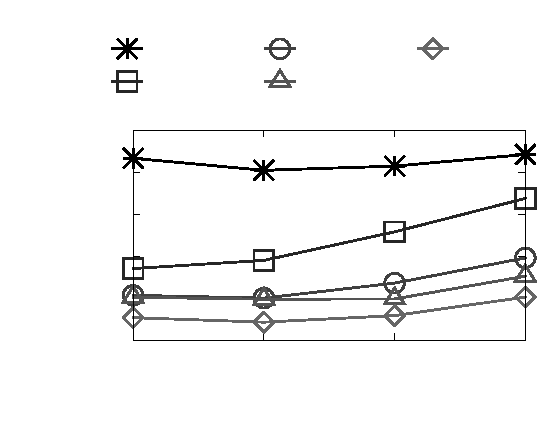
\includegraphics{scattershared}}%
    \gplfronttext
  \end{picture}%
\endgroup
}
\caption{Symbolic $\ACIFn{}(\loadVar)$}
\label{fig:scatter:jaccard:sharedsymload}
\end{subfigure}%
\hfill
\begin{subfigure}[t]{0.49\columnwidth}
\resizebox{\linewidth}{!}{\protect\small% GNUPLOT: LaTeX picture with Postscript
\begingroup
  \fontfamily{Times-Roman}%
  \selectfont
  \makeatletter
  \providecommand\color[2][]{%
    \GenericError{(gnuplot) \space\space\space\@spaces}{%
      Package color not loaded in conjunction with
      terminal option `colourtext'%
    }{See the gnuplot documentation for explanation.%
    }{Either use 'blacktext' in gnuplot or load the package
      color.sty in LaTeX.}%
    \renewcommand\color[2][]{}%
  }%
  \providecommand\includegraphics[2][]{%
    \GenericError{(gnuplot) \space\space\space\@spaces}{%
      Package graphicx or graphics not loaded%
    }{See the gnuplot documentation for explanation.%
    }{The gnuplot epslatex terminal needs graphicx.sty or graphics.sty.}%
    \renewcommand\includegraphics[2][]{}%
  }%
  \providecommand\rotatebox[2]{#2}%
  \@ifundefined{ifGPcolor}{%
    \newif\ifGPcolor
    \GPcolortrue
  }{}%
  \@ifundefined{ifGPblacktext}{%
    \newif\ifGPblacktext
    \GPblacktexttrue
  }{}%
  % define a \g@addto@macro without @ in the name:
  \let\gplgaddtomacro\g@addto@macro
  % define empty templates for all commands taking text:
  \gdef\gplbacktext{}%
  \gdef\gplfronttext{}%
  \makeatother
  \ifGPblacktext
    % no textcolor at all
    \def\colorrgb#1{}%
    \def\colorgray#1{}%
  \else
    % gray or color?
    \ifGPcolor
      \def\colorrgb#1{\color[rgb]{#1}}%
      \def\colorgray#1{\color[gray]{#1}}%
      \expandafter\def\csname LTw\endcsname{\color{white}}%
      \expandafter\def\csname LTb\endcsname{\color{black}}%
      \expandafter\def\csname LTa\endcsname{\color{black}}%
      \expandafter\def\csname LT0\endcsname{\color[rgb]{1,0,0}}%
      \expandafter\def\csname LT1\endcsname{\color[rgb]{0,1,0}}%
      \expandafter\def\csname LT2\endcsname{\color[rgb]{0,0,1}}%
      \expandafter\def\csname LT3\endcsname{\color[rgb]{1,0,1}}%
      \expandafter\def\csname LT4\endcsname{\color[rgb]{0,1,1}}%
      \expandafter\def\csname LT5\endcsname{\color[rgb]{1,1,0}}%
      \expandafter\def\csname LT6\endcsname{\color[rgb]{0,0,0}}%
      \expandafter\def\csname LT7\endcsname{\color[rgb]{1,0.3,0}}%
      \expandafter\def\csname LT8\endcsname{\color[rgb]{0.5,0.5,0.5}}%
    \else
      % gray
      \def\colorrgb#1{\color{black}}%
      \def\colorgray#1{\color[gray]{#1}}%
      \expandafter\def\csname LTw\endcsname{\color{white}}%
      \expandafter\def\csname LTb\endcsname{\color{black}}%
      \expandafter\def\csname LTa\endcsname{\color{black}}%
      \expandafter\def\csname LT0\endcsname{\color{black}}%
      \expandafter\def\csname LT1\endcsname{\color{black}}%
      \expandafter\def\csname LT2\endcsname{\color{black}}%
      \expandafter\def\csname LT3\endcsname{\color{black}}%
      \expandafter\def\csname LT4\endcsname{\color{black}}%
      \expandafter\def\csname LT5\endcsname{\color{black}}%
      \expandafter\def\csname LT6\endcsname{\color{black}}%
      \expandafter\def\csname LT7\endcsname{\color{black}}%
      \expandafter\def\csname LT8\endcsname{\color{black}}%
    \fi
  \fi
    \setlength{\unitlength}{0.0500bp}%
    \ifx\gptboxheight\undefined%
      \newlength{\gptboxheight}%
      \newlength{\gptboxwidth}%
      \newsavebox{\gptboxtext}%
    \fi%
    \setlength{\fboxrule}{0.5pt}%
    \setlength{\fboxsep}{1pt}%
\begin{picture}(5040.00,3888.00)%
    \gplgaddtomacro\gplbacktext{%
      \csname LTb\endcsname%%
      \put(962,780){\makebox(0,0)[r]{\strut{}$0$}}%
      \put(962,1183){\makebox(0,0)[r]{\strut{}$0.2$}}%
      \put(962,1586){\makebox(0,0)[r]{\strut{}$0.4$}}%
      \put(962,1989){\makebox(0,0)[r]{\strut{}$0.6$}}%
      \put(962,2392){\makebox(0,0)[r]{\strut{}$0.8$}}%
      \put(962,2795){\makebox(0,0)[r]{\strut{}$1$}}%
      \put(1118,520){\makebox(0,0){\strut{}$0$}}%
      \put(2373,520){\makebox(0,0){\strut{}$1$}}%
      \put(3628,520){\makebox(0,0){\strut{}$2$}}%
      \put(4883,520){\makebox(0,0){\strut{}$3$}}%
    }%
    \gplgaddtomacro\gplfronttext{%
      \csname LTb\endcsname%%
      \put(309,1787){\rotatebox{-270}{\makebox(0,0){\strut{}\JaccardRand{\secretsSetSize}}}}%
      \put(3000,182){\makebox(0,0){\strut{}$\log_2{\secretsSetSize}$}}%
      \csname LTb\endcsname%%
      \put(1365,3576){\makebox(0,0)[l]{\strut{}$\cachesetNmbr=1$}}%
      \csname LTb\endcsname%%
      \put(1365,3264){\makebox(0,0)[l]{\strut{}$\cachesetNmbr=2$}}%
      \csname LTb\endcsname%%
      \put(2832,3576){\makebox(0,0)[l]{\strut{}$\cachesetNmbr=4$}}%
      \csname LTb\endcsname%%
      \put(2832,3264){\makebox(0,0)[l]{\strut{}$\cachesetNmbr=8$}}%
      \csname LTb\endcsname%%
      \put(4299,3576){\makebox(0,0)[l]{\strut{}$\cachesetNmbr=16$}}%
    }%
    \gplbacktext
    \put(0,0){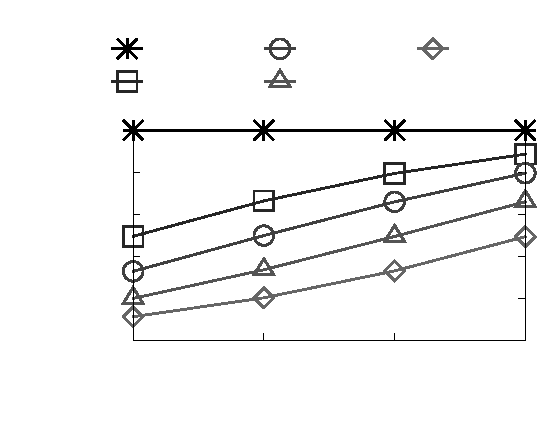
\includegraphics{scatterflushreload}}%
    \gplfronttext
  \end{picture}%
\endgroup
}
\caption{$\forall \blockIdx: \ACIFn{}(\loadVar)[\blockIdx] = 0$}
\label{fig:scatter:jaccard:flushreload}
\end{subfigure}%
\caption{\scatterCache, unknown \cacheMap{\domainIdx}, memory
  sharing enabled (\flushreload attack)\label{fig:scatter:jaccard:shared}}
\end{figure}

\begin{figure}[t]
\begin{subfigure}[t]{0.49\columnwidth}
\resizebox{\linewidth}{!}{\protect\small% GNUPLOT: LaTeX picture with Postscript
\begingroup
  \fontfamily{Times-Roman}%
  \selectfont
  \makeatletter
  \providecommand\color[2][]{%
    \GenericError{(gnuplot) \space\space\space\@spaces}{%
      Package color not loaded in conjunction with
      terminal option `colourtext'%
    }{See the gnuplot documentation for explanation.%
    }{Either use 'blacktext' in gnuplot or load the package
      color.sty in LaTeX.}%
    \renewcommand\color[2][]{}%
  }%
  \providecommand\includegraphics[2][]{%
    \GenericError{(gnuplot) \space\space\space\@spaces}{%
      Package graphicx or graphics not loaded%
    }{See the gnuplot documentation for explanation.%
    }{The gnuplot epslatex terminal needs graphicx.sty or graphics.sty.}%
    \renewcommand\includegraphics[2][]{}%
  }%
  \providecommand\rotatebox[2]{#2}%
  \@ifundefined{ifGPcolor}{%
    \newif\ifGPcolor
    \GPcolortrue
  }{}%
  \@ifundefined{ifGPblacktext}{%
    \newif\ifGPblacktext
    \GPblacktexttrue
  }{}%
  % define a \g@addto@macro without @ in the name:
  \let\gplgaddtomacro\g@addto@macro
  % define empty templates for all commands taking text:
  \gdef\gplbacktext{}%
  \gdef\gplfronttext{}%
  \makeatother
  \ifGPblacktext
    % no textcolor at all
    \def\colorrgb#1{}%
    \def\colorgray#1{}%
  \else
    % gray or color?
    \ifGPcolor
      \def\colorrgb#1{\color[rgb]{#1}}%
      \def\colorgray#1{\color[gray]{#1}}%
      \expandafter\def\csname LTw\endcsname{\color{white}}%
      \expandafter\def\csname LTb\endcsname{\color{black}}%
      \expandafter\def\csname LTa\endcsname{\color{black}}%
      \expandafter\def\csname LT0\endcsname{\color[rgb]{1,0,0}}%
      \expandafter\def\csname LT1\endcsname{\color[rgb]{0,1,0}}%
      \expandafter\def\csname LT2\endcsname{\color[rgb]{0,0,1}}%
      \expandafter\def\csname LT3\endcsname{\color[rgb]{1,0,1}}%
      \expandafter\def\csname LT4\endcsname{\color[rgb]{0,1,1}}%
      \expandafter\def\csname LT5\endcsname{\color[rgb]{1,1,0}}%
      \expandafter\def\csname LT6\endcsname{\color[rgb]{0,0,0}}%
      \expandafter\def\csname LT7\endcsname{\color[rgb]{1,0.3,0}}%
      \expandafter\def\csname LT8\endcsname{\color[rgb]{0.5,0.5,0.5}}%
    \else
      % gray
      \def\colorrgb#1{\color{black}}%
      \def\colorgray#1{\color[gray]{#1}}%
      \expandafter\def\csname LTw\endcsname{\color{white}}%
      \expandafter\def\csname LTb\endcsname{\color{black}}%
      \expandafter\def\csname LTa\endcsname{\color{black}}%
      \expandafter\def\csname LT0\endcsname{\color{black}}%
      \expandafter\def\csname LT1\endcsname{\color{black}}%
      \expandafter\def\csname LT2\endcsname{\color{black}}%
      \expandafter\def\csname LT3\endcsname{\color{black}}%
      \expandafter\def\csname LT4\endcsname{\color{black}}%
      \expandafter\def\csname LT5\endcsname{\color{black}}%
      \expandafter\def\csname LT6\endcsname{\color{black}}%
      \expandafter\def\csname LT7\endcsname{\color{black}}%
      \expandafter\def\csname LT8\endcsname{\color{black}}%
    \fi
  \fi
    \setlength{\unitlength}{0.0500bp}%
    \ifx\gptboxheight\undefined%
      \newlength{\gptboxheight}%
      \newlength{\gptboxwidth}%
      \newsavebox{\gptboxtext}%
    \fi%
    \setlength{\fboxrule}{0.5pt}%
    \setlength{\fboxsep}{1pt}%
\begin{picture}(5040.00,3888.00)%
    \gplgaddtomacro\gplbacktext{%
      \csname LTb\endcsname%%
      \put(962,780){\makebox(0,0)[r]{\strut{}$0$}}%
      \put(962,1183){\makebox(0,0)[r]{\strut{}$0.2$}}%
      \put(962,1586){\makebox(0,0)[r]{\strut{}$0.4$}}%
      \put(962,1989){\makebox(0,0)[r]{\strut{}$0.6$}}%
      \put(962,2392){\makebox(0,0)[r]{\strut{}$0.8$}}%
      \put(962,2795){\makebox(0,0)[r]{\strut{}$1$}}%
      \put(1118,520){\makebox(0,0){\strut{}$0$}}%
      \put(2373,520){\makebox(0,0){\strut{}$1$}}%
      \put(3628,520){\makebox(0,0){\strut{}$2$}}%
      \put(4883,520){\makebox(0,0){\strut{}$3$}}%
    }%
    \gplgaddtomacro\gplfronttext{%
      \csname LTb\endcsname%%
      \put(309,1787){\rotatebox{-270}{\makebox(0,0){\strut{}\JaccardRand{\secretsSetSize}}}}%
      \put(3000,182){\makebox(0,0){\strut{}$\log_2{\secretsSetSize}$}}%
      \csname LTb\endcsname%%
      \put(1365,3653){\makebox(0,0)[l]{\strut{}$\cachesetNmbr=1,\phantomR=1$}}%
      \csname LTb\endcsname%%
      \put(1365,3341){\makebox(0,0)[l]{\strut{}$\cachesetNmbr=4,\phantomR=1$}}%
      \csname LTb\endcsname%%
      \put(1365,3029){\makebox(0,0)[l]{\strut{}$\cachesetNmbr=4,\phantomR=2$}}%
      \csname LTb\endcsname%%
      \put(3534,3653){\makebox(0,0)[l]{\strut{}$\cachesetNmbr=8,\phantomR=1$}}%
      \csname LTb\endcsname%%
      \put(3534,3341){\makebox(0,0)[l]{\strut{}$\cachesetNmbr=8,\phantomR=2$}}%
      \csname LTb\endcsname%%
      \put(3534,3029){\makebox(0,0)[l]{\strut{}$\cachesetNmbr=16,\phantomR=1$}}%
    }%
    \gplbacktext
    \put(0,0){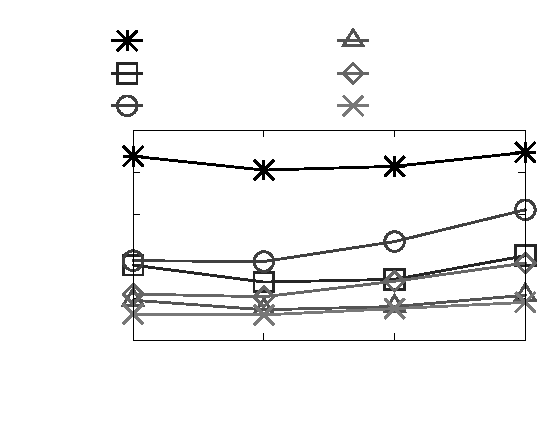
\includegraphics{phantomshared}}%
    \gplfronttext
  \end{picture}%
\endgroup
}
\caption{Symbolic $\ACIFn{}(\loadVar)$}
\label{fig:phantom:jaccard:sharedsymload}
\end{subfigure}%
\hfill
\begin{subfigure}[t]{0.49\columnwidth}
\resizebox{\linewidth}{!}{\protect\small% GNUPLOT: LaTeX picture with Postscript
\begingroup
  \fontfamily{Times-Roman}%
  \selectfont
  \makeatletter
  \providecommand\color[2][]{%
    \GenericError{(gnuplot) \space\space\space\@spaces}{%
      Package color not loaded in conjunction with
      terminal option `colourtext'%
    }{See the gnuplot documentation for explanation.%
    }{Either use 'blacktext' in gnuplot or load the package
      color.sty in LaTeX.}%
    \renewcommand\color[2][]{}%
  }%
  \providecommand\includegraphics[2][]{%
    \GenericError{(gnuplot) \space\space\space\@spaces}{%
      Package graphicx or graphics not loaded%
    }{See the gnuplot documentation for explanation.%
    }{The gnuplot epslatex terminal needs graphicx.sty or graphics.sty.}%
    \renewcommand\includegraphics[2][]{}%
  }%
  \providecommand\rotatebox[2]{#2}%
  \@ifundefined{ifGPcolor}{%
    \newif\ifGPcolor
    \GPcolortrue
  }{}%
  \@ifundefined{ifGPblacktext}{%
    \newif\ifGPblacktext
    \GPblacktexttrue
  }{}%
  % define a \g@addto@macro without @ in the name:
  \let\gplgaddtomacro\g@addto@macro
  % define empty templates for all commands taking text:
  \gdef\gplbacktext{}%
  \gdef\gplfronttext{}%
  \makeatother
  \ifGPblacktext
    % no textcolor at all
    \def\colorrgb#1{}%
    \def\colorgray#1{}%
  \else
    % gray or color?
    \ifGPcolor
      \def\colorrgb#1{\color[rgb]{#1}}%
      \def\colorgray#1{\color[gray]{#1}}%
      \expandafter\def\csname LTw\endcsname{\color{white}}%
      \expandafter\def\csname LTb\endcsname{\color{black}}%
      \expandafter\def\csname LTa\endcsname{\color{black}}%
      \expandafter\def\csname LT0\endcsname{\color[rgb]{1,0,0}}%
      \expandafter\def\csname LT1\endcsname{\color[rgb]{0,1,0}}%
      \expandafter\def\csname LT2\endcsname{\color[rgb]{0,0,1}}%
      \expandafter\def\csname LT3\endcsname{\color[rgb]{1,0,1}}%
      \expandafter\def\csname LT4\endcsname{\color[rgb]{0,1,1}}%
      \expandafter\def\csname LT5\endcsname{\color[rgb]{1,1,0}}%
      \expandafter\def\csname LT6\endcsname{\color[rgb]{0,0,0}}%
      \expandafter\def\csname LT7\endcsname{\color[rgb]{1,0.3,0}}%
      \expandafter\def\csname LT8\endcsname{\color[rgb]{0.5,0.5,0.5}}%
    \else
      % gray
      \def\colorrgb#1{\color{black}}%
      \def\colorgray#1{\color[gray]{#1}}%
      \expandafter\def\csname LTw\endcsname{\color{white}}%
      \expandafter\def\csname LTb\endcsname{\color{black}}%
      \expandafter\def\csname LTa\endcsname{\color{black}}%
      \expandafter\def\csname LT0\endcsname{\color{black}}%
      \expandafter\def\csname LT1\endcsname{\color{black}}%
      \expandafter\def\csname LT2\endcsname{\color{black}}%
      \expandafter\def\csname LT3\endcsname{\color{black}}%
      \expandafter\def\csname LT4\endcsname{\color{black}}%
      \expandafter\def\csname LT5\endcsname{\color{black}}%
      \expandafter\def\csname LT6\endcsname{\color{black}}%
      \expandafter\def\csname LT7\endcsname{\color{black}}%
      \expandafter\def\csname LT8\endcsname{\color{black}}%
    \fi
  \fi
    \setlength{\unitlength}{0.0500bp}%
    \ifx\gptboxheight\undefined%
      \newlength{\gptboxheight}%
      \newlength{\gptboxwidth}%
      \newsavebox{\gptboxtext}%
    \fi%
    \setlength{\fboxrule}{0.5pt}%
    \setlength{\fboxsep}{1pt}%
\begin{picture}(5040.00,3888.00)%
    \gplgaddtomacro\gplbacktext{%
      \csname LTb\endcsname%%
      \put(962,780){\makebox(0,0)[r]{\strut{}$0$}}%
      \put(962,1183){\makebox(0,0)[r]{\strut{}$0.2$}}%
      \put(962,1586){\makebox(0,0)[r]{\strut{}$0.4$}}%
      \put(962,1989){\makebox(0,0)[r]{\strut{}$0.6$}}%
      \put(962,2392){\makebox(0,0)[r]{\strut{}$0.8$}}%
      \put(962,2795){\makebox(0,0)[r]{\strut{}$1$}}%
      \put(1118,520){\makebox(0,0){\strut{}$0$}}%
      \put(2373,520){\makebox(0,0){\strut{}$1$}}%
      \put(3628,520){\makebox(0,0){\strut{}$2$}}%
      \put(4883,520){\makebox(0,0){\strut{}$3$}}%
    }%
    \gplgaddtomacro\gplfronttext{%
      \csname LTb\endcsname%%
      \put(309,1787){\rotatebox{-270}{\makebox(0,0){\strut{}\JaccardRand{\secretsSetSize}}}}%
      \put(3000,182){\makebox(0,0){\strut{}$\log_2{\secretsSetSize}$}}%
      \csname LTb\endcsname%%
      \put(1365,3653){\makebox(0,0)[l]{\strut{}$\cachesetNmbr=1,\phantomR=1$}}%
      \csname LTb\endcsname%%
      \put(1365,3341){\makebox(0,0)[l]{\strut{}$\cachesetNmbr=4,\phantomR=1$}}%
      \csname LTb\endcsname%%
      \put(1365,3029){\makebox(0,0)[l]{\strut{}$\cachesetNmbr=4,\phantomR=2$}}%
      \csname LTb\endcsname%%
      \put(3534,3653){\makebox(0,0)[l]{\strut{}$\cachesetNmbr=8,\phantomR=1$}}%
      \csname LTb\endcsname%%
      \put(3534,3341){\makebox(0,0)[l]{\strut{}$\cachesetNmbr=8,\phantomR=2$}}%
      \csname LTb\endcsname%%
      \put(3534,3029){\makebox(0,0)[l]{\strut{}$\cachesetNmbr=16,\phantomR=1$}}%
    }%
    \gplbacktext
    \put(0,0){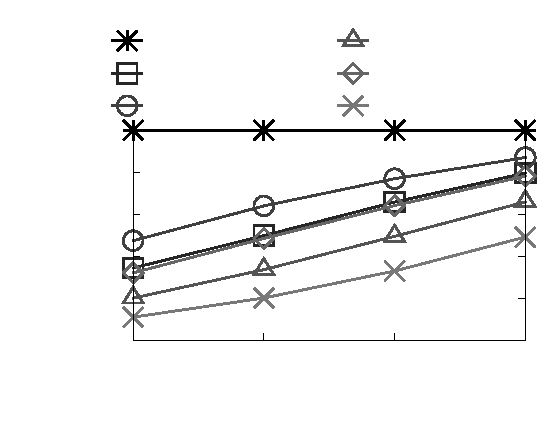
\includegraphics{phantomflushreload}}%
    \gplfronttext
  \end{picture}%
\endgroup
}
\caption{$\forall \blockIdx: \ACIFn{}(\loadVar)[\blockIdx] = 0$}
\label{fig:phantom:jaccard:flushreload}
\end{subfigure}%
\caption{\phantomCache, unknown \phantomCacheMap{\domainIdx},
  memory sharing enabled (\flushreload attack)
  \label{fig:phantom:jaccard:shared}}
\end{figure}
\label{dinome:sec:cacheMitigations:random}
First, we experimented without memory sharing when assuming the
memory-to-cache mapping is completely unknown to the attacker.  We
ended up with $\JaccardRand{\secretsSetSize}=0$ for all
\secretsSetSize in both \scatterCache and \phantomCache. The attacker
cannot tell which memory blocks are accessed by the victim, as an
memory block could be mapped to any cache line if the mapping is
unknown. However, with shared memory, shown in
\figref{fig:scatter:jaccard:sharedsymload} and
\figref{fig:scatter:jaccard:flushreload}, it is still possible to
learn some information about which memory block is accessed by the
victim. \JaccardRand{\secretsSetSize} is high when \secretsSetSize is
large, indicating the attacker can precisely determine
$\SecFn{}(\secretVar)$ when leakage occurs.  Our results indicate that
lower cache set granularity leaks more: In
\figref{fig:scatter:jaccard:sharedsymload}, $\cachesetNmbr=1$ leaks
the most, which is similar to the normal cache.  When
$\cachesetNmbr>1$, the leakage is reduced.

Overall, with same cache set granularity,
\JaccardRand{\secretsSetSize} is higher with \phantomCache with
$\phantomR=2$ than \phantomCache with $\phantomR=1$ and \scatterCache
when memory is shared. This is because setting $\phantomR=2$ allows
one physical address to be mapped to more cache sets and so gains more
chance to share cache lines cross domains.

Intuitively, \flushreload is the best attacker strategy for a normal
cache design when memory sharing is enabled.  However, for a new cache
design, it may not be clear that it is still the best.  Our leakage
rules provide some insight for \scatterCache and \phantomCache.  For
example, two top-ranking rules for \scatterCache, both with precision
$\ge 0.80$ and recall of $\approx 0.02$, are:
\begin{align}
  {\small\begin{array}{rrrrrrrr}
    & \SecFn{}(\secretVar)[3]\ge 1 & \wedge
    & \SecFn{}(\secretVar)[2]<1 
    \wedge
    & \SecFn{}(\secretVar)[1]<1 & \wedge
     \SecFn{}(\secretVar)[0]<1 \\
    \wedge
    & \AIIFn{}(\cacheMapEntry{\victimDomainId}{8}{1}) \ge 5 & \wedge
    & \AIIFn{}(\cacheMapEntry{\attackerDomainId}{8}{1}) \ge 5 
    \wedge
    & \ACIFn{}(\loadVar)[8]<1
  \end{array}} \label{eqn:scatter-interference-ruleOne}
\if 0
\\
  {\small\begin{array}{rrrrrrrr}
    & \SecFn{}(\secretVar)[0]<1 & \wedge
    & \SecFn{}(\secretVar)\ge 10 \\
    \wedge
    & \SecFn{}(\secretVar)<12 & \wedge
    & \AIIFn{}(\cacheMapEntry{\victimDomainId}{10}{0}) \ge 5 \\
    \wedge
    & \AIIFn{}(\cacheMapEntry{\attackerDomainId}{10}{0}) \ge 5 & \wedge
    & \ACIFn{}(\loadVar)[10]<1
  \end{array}} \label{eqn:scatter-interference-ruleTwo}
\fi
\end{align}
These rules are similar to \eqref{eqn:flush-reload-interference} but
with some additional predicates about
\cacheMap{\victimDomainId}. Specifically,
\eqnref{eqn:scatter-interference-ruleOne} adds
$\AIIFn{}(\cacheMapEntry{\victimDomainId}{8}{1})\ge 5 \wedge
\AIIFn{}(\cacheMapEntry{\attackerDomainId}{8}{1})\ge 5$ to the rule
when setting $\ACIFn{}(\loadVar)[8]=0$ (i.e., attacker \Flush{es}
\block{8}) and $\SecFn{}(\secretVar) = 8$, which indicates that the
\block{8} should occupy line $\wayIdx=1$ in set $\cachesetIdx=5$ in
both the victim's and attacker's domains to ensure leakage about
whether $\SecFn{}(\secretVar) = 8$ when the attacker \Reload{s}
\block{8}. 

Thus, an attacker should \flushreload all blocks that could share
cache lines between victim's and attacker's domain to cause more
leakage.  Since the memory-to-cache mapping is unknown, an attacker
may \flushreload all shared memory blocks. The resulting
\JaccardRand{\secretsSetSize} is shown in
\figref{fig:scatter:jaccard:flushreload} for \scatterCache and
\figref{fig:phantom:jaccard:flushreload} for \phantomCache. Under the
equivalent cache settings, \JaccardRand{\secretsSetSize} is higher
when the attacker takes maximum advantage of \flushreload attacks
(versus not, shown in \figref{fig:scatter:jaccard:sharedsymload} and
\figref{fig:phantom:jaccard:sharedsymload}).  We also see that
\JaccardRand{\secretsSetSize} for `$\cachesetNmbr=8,\phantomR=2$' is
close to that for `$\cachesetNmbr=4,\phantomR=1$', as randomly mapping
to 2 out of 8 sets is similar to mapping to 1 out of 4 cache sets.
Our evaluation results suggests that \scatterCache and \phantomCache
eliminate side-channel leakage when there is no shared memory and
largely restrict it when there is shared memory, if the
address-to-cache mapping is random and remains unknown to the
attacker.

\iffalse
\begin{table}
\caption{Selected interference rules for \scatterCache w/ memory sharing\label{tab:scatter:shared}}
\scriptsize{
\begingroup
\everymath{\scriptstyle}
\footnotesize
%your equation
\begin{tabular}{m{\colR}m{\colRule}m{\colPrecision}m{\colRecall}}
\toprule
 & Interference rules (\interferenceRule{}) & Precision & Recall \\
\midrule
$\interferenceRule{0}$&$\SecFn{}(\secretVar)[3]\ge 1 \wedge
\SecFn{}(\secretVar)[2]<1 \wedge \SecFn{}(\secretVar)[1]<1 \wedge
\SecFn{}(\secretVar)[0]<1 \wedge
\AIIFn{}(\cacheMapEntry{\victimDomainId}{8}{1})
\ge 5 \wedge \AIIFn{}(\cacheMapEntry{\attackerDomainId}{8}{1}) \ge 5 \wedge \ACIFn{}(\loadVar)[8]<1$&0.81&0.02\\
$\interferenceRule{1}$&$\SecFn{}(\secretVar)[0]<1 \wedge
\SecFn{}(\secretVar)\ge 10 \wedge \SecFn{}(\secretVar)<12
\wedge \AIIFn{}(\cacheMapEntry{\victimDomainId}{10}{0}) \ge 5 \wedge
\AIIFn{}(\cacheMapEntry{\attackerDomainId}{10}{0}) \ge 5 \wedge \ACIFn{}(\loadVar)[10]<
1$&0.80&0.02\\
\if0
$\interferenceRule{2}$&$\SecFn{}(\secretVar)[3]<1 \wedge
\SecFn{}(\secretVar)[0]\ge 1 \wedge \SecFn{}(\secretVar)\ge 6 \wedge
\AIIFn{}(\cacheMapEntry{\vitimDomainIdx}{7}{1})[1]\ge 1 \wedge
\AIIFn{}(\cacheMapEntry{\attackerDomainId}{7}{1})[1]\ge 1 \wedge
\ACIFn{}(\loadVar)[7]<1 $&0.77&0.01\\
$\interferenceRule{3}$&$\SecFn{}(\secretVar)[3]<1 \wedge
\SecFn{}(\secretVar)[2]\ge 1 \wedge \SecFn{}(\secretVar)[1]<1 \wedge
\SecFn{}(\secretVar)[0]\ge 1 \wedge
\AIIFn{}(\cacheMapEntry{\victimDomainId}{5}{1})[1]<1 \wedge
\AIIFn{}(\cacheMapEntry{\attackerDomainId}{5}{1})[1]<1 \wedge \ACIFn{}(\loadVar)[5]<1$&0.77&0.03\\
$\interferenceRule{4}$&$\SecFn{}(\secretVar)[2]\ge 1 \wedge
\SecFn{}(\secretVar)[0]\ge 1 \wedge \SecFn{}(\secretVar)<6 \wedge
\AIIFn{}(\cacheMapEntry{\victimDomainId}{5}{1})[0]\ge 1 \wedge
\AIIFn{}(\cacheMapEntry{\attackerDomainId}{5}{1})[0]\ge 1 \wedge \ACIFn{}(\loadVar)[5]<1$&0.76&0.02\\
$\interferenceRule{5}$&$\SecFn{}(\secretVar)[3]\ge 1 \wedge
\SecFn{}(\secretVar)[2]<1 \wedge \SecFn{}(\secretVar)[1]\ge 1 \wedge
\SecFn{}(\secretVar)[0]<1 \wedge
\AIIFn{}(\cacheMap{\victimDomainId}{10}{0})[0]\ge 1 \wedge
\AIIFn{}(\cacheMapEntry{\attackerDomainId}{10}{0})[0]\ge 1 \wedge \ACIFn{}(\loadVar)[10]<1$&0.76&0.02\\
\fi
\bottomrule
\end{tabular}
\endgroup
}
\end{table}
\fi


\subsubsection{Declassifying the memory-to-cache mapping}
\begin{figure}
\begin{subfigure}[t]{0.495\linewidth}
\resizebox{\linewidth}{!}{\protect\small% GNUPLOT: LaTeX picture with Postscript
\begingroup
  \fontfamily{Times-Roman}%
  \selectfont
  \makeatletter
  \providecommand\color[2][]{%
    \GenericError{(gnuplot) \space\space\space\@spaces}{%
      Package color not loaded in conjunction with
      terminal option `colourtext'%
    }{See the gnuplot documentation for explanation.%
    }{Either use 'blacktext' in gnuplot or load the package
      color.sty in LaTeX.}%
    \renewcommand\color[2][]{}%
  }%
  \providecommand\includegraphics[2][]{%
    \GenericError{(gnuplot) \space\space\space\@spaces}{%
      Package graphicx or graphics not loaded%
    }{See the gnuplot documentation for explanation.%
    }{The gnuplot epslatex terminal needs graphicx.sty or graphics.sty.}%
    \renewcommand\includegraphics[2][]{}%
  }%
  \providecommand\rotatebox[2]{#2}%
  \@ifundefined{ifGPcolor}{%
    \newif\ifGPcolor
    \GPcolortrue
  }{}%
  \@ifundefined{ifGPblacktext}{%
    \newif\ifGPblacktext
    \GPblacktexttrue
  }{}%
  % define a \g@addto@macro without @ in the name:
  \let\gplgaddtomacro\g@addto@macro
  % define empty templates for all commands taking text:
  \gdef\gplbacktext{}%
  \gdef\gplfronttext{}%
  \makeatother
  \ifGPblacktext
    % no textcolor at all
    \def\colorrgb#1{}%
    \def\colorgray#1{}%
  \else
    % gray or color?
    \ifGPcolor
      \def\colorrgb#1{\color[rgb]{#1}}%
      \def\colorgray#1{\color[gray]{#1}}%
      \expandafter\def\csname LTw\endcsname{\color{white}}%
      \expandafter\def\csname LTb\endcsname{\color{black}}%
      \expandafter\def\csname LTa\endcsname{\color{black}}%
      \expandafter\def\csname LT0\endcsname{\color[rgb]{1,0,0}}%
      \expandafter\def\csname LT1\endcsname{\color[rgb]{0,1,0}}%
      \expandafter\def\csname LT2\endcsname{\color[rgb]{0,0,1}}%
      \expandafter\def\csname LT3\endcsname{\color[rgb]{1,0,1}}%
      \expandafter\def\csname LT4\endcsname{\color[rgb]{0,1,1}}%
      \expandafter\def\csname LT5\endcsname{\color[rgb]{1,1,0}}%
      \expandafter\def\csname LT6\endcsname{\color[rgb]{0,0,0}}%
      \expandafter\def\csname LT7\endcsname{\color[rgb]{1,0.3,0}}%
      \expandafter\def\csname LT8\endcsname{\color[rgb]{0.5,0.5,0.5}}%
    \else
      % gray
      \def\colorrgb#1{\color{black}}%
      \def\colorgray#1{\color[gray]{#1}}%
      \expandafter\def\csname LTw\endcsname{\color{white}}%
      \expandafter\def\csname LTb\endcsname{\color{black}}%
      \expandafter\def\csname LTa\endcsname{\color{black}}%
      \expandafter\def\csname LT0\endcsname{\color{black}}%
      \expandafter\def\csname LT1\endcsname{\color{black}}%
      \expandafter\def\csname LT2\endcsname{\color{black}}%
      \expandafter\def\csname LT3\endcsname{\color{black}}%
      \expandafter\def\csname LT4\endcsname{\color{black}}%
      \expandafter\def\csname LT5\endcsname{\color{black}}%
      \expandafter\def\csname LT6\endcsname{\color{black}}%
      \expandafter\def\csname LT7\endcsname{\color{black}}%
      \expandafter\def\csname LT8\endcsname{\color{black}}%
    \fi
  \fi
    \setlength{\unitlength}{0.0500bp}%
    \ifx\gptboxheight\undefined%
      \newlength{\gptboxheight}%
      \newlength{\gptboxwidth}%
      \newsavebox{\gptboxtext}%
    \fi%
    \setlength{\fboxrule}{0.5pt}%
    \setlength{\fboxsep}{1pt}%
\begin{picture}(5040.00,3888.00)%
    \gplgaddtomacro\gplbacktext{%
      \csname LTb\endcsname%%
      \put(962,780){\makebox(0,0)[r]{\strut{}$0$}}%
      \put(962,1183){\makebox(0,0)[r]{\strut{}$0.2$}}%
      \put(962,1586){\makebox(0,0)[r]{\strut{}$0.4$}}%
      \put(962,1989){\makebox(0,0)[r]{\strut{}$0.6$}}%
      \put(962,2392){\makebox(0,0)[r]{\strut{}$0.8$}}%
      \put(962,2795){\makebox(0,0)[r]{\strut{}$1$}}%
      \put(1118,520){\makebox(0,0){\strut{}$0$}}%
      \put(2373,520){\makebox(0,0){\strut{}$1$}}%
      \put(3628,520){\makebox(0,0){\strut{}$2$}}%
      \put(4883,520){\makebox(0,0){\strut{}$3$}}%
    }%
    \gplgaddtomacro\gplfronttext{%
      \csname LTb\endcsname%%
      \put(309,1787){\rotatebox{-270}{\makebox(0,0){\strut{}\JaccardWithDeclass{\secretsSetSize}}}}%
      \put(3000,182){\makebox(0,0){\strut{}$\log_2{\secretsSetSize}$}}%
      \csname LTb\endcsname%%
      \put(1365,3576){\makebox(0,0)[l]{\strut{}$\cachesetNmbr=1$}}%
      \csname LTb\endcsname%%
      \put(1365,3264){\makebox(0,0)[l]{\strut{}$\cachesetNmbr=2$}}%
      \csname LTb\endcsname%%
      \put(2832,3576){\makebox(0,0)[l]{\strut{}$\cachesetNmbr=4$}}%
      \csname LTb\endcsname%%
      \put(2832,3264){\makebox(0,0)[l]{\strut{}$\cachesetNmbr=8$}}%
      \csname LTb\endcsname%%
      \put(4299,3576){\makebox(0,0)[l]{\strut{}$\cachesetNmbr=16$}}%
    }%
    \gplbacktext
    \put(0,0){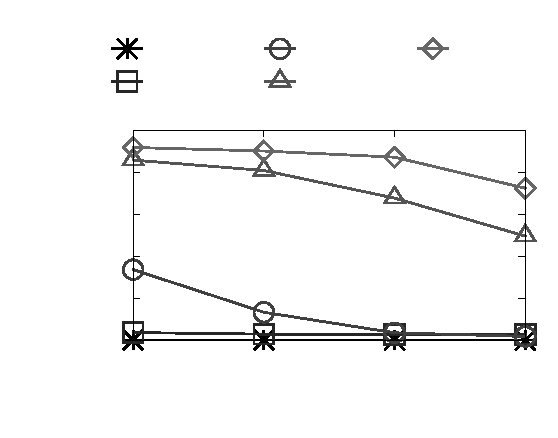
\includegraphics{scatterprimeprobe-declass}}%
    \gplfronttext
  \end{picture}%
\endgroup
}
\caption{\scatterCache
\label{fig:scatter:jaccard:primeprobe:declass}}
\end{subfigure}%
\begin{subfigure}[t]{0.495\linewidth}
\resizebox{\linewidth}{!}{\protect\small% GNUPLOT: LaTeX picture with Postscript
\begingroup
  \fontfamily{Times-Roman}%
  \selectfont
  \makeatletter
  \providecommand\color[2][]{%
    \GenericError{(gnuplot) \space\space\space\@spaces}{%
      Package color not loaded in conjunction with
      terminal option `colourtext'%
    }{See the gnuplot documentation for explanation.%
    }{Either use 'blacktext' in gnuplot or load the package
      color.sty in LaTeX.}%
    \renewcommand\color[2][]{}%
  }%
  \providecommand\includegraphics[2][]{%
    \GenericError{(gnuplot) \space\space\space\@spaces}{%
      Package graphicx or graphics not loaded%
    }{See the gnuplot documentation for explanation.%
    }{The gnuplot epslatex terminal needs graphicx.sty or graphics.sty.}%
    \renewcommand\includegraphics[2][]{}%
  }%
  \providecommand\rotatebox[2]{#2}%
  \@ifundefined{ifGPcolor}{%
    \newif\ifGPcolor
    \GPcolortrue
  }{}%
  \@ifundefined{ifGPblacktext}{%
    \newif\ifGPblacktext
    \GPblacktexttrue
  }{}%
  % define a \g@addto@macro without @ in the name:
  \let\gplgaddtomacro\g@addto@macro
  % define empty templates for all commands taking text:
  \gdef\gplbacktext{}%
  \gdef\gplfronttext{}%
  \makeatother
  \ifGPblacktext
    % no textcolor at all
    \def\colorrgb#1{}%
    \def\colorgray#1{}%
  \else
    % gray or color?
    \ifGPcolor
      \def\colorrgb#1{\color[rgb]{#1}}%
      \def\colorgray#1{\color[gray]{#1}}%
      \expandafter\def\csname LTw\endcsname{\color{white}}%
      \expandafter\def\csname LTb\endcsname{\color{black}}%
      \expandafter\def\csname LTa\endcsname{\color{black}}%
      \expandafter\def\csname LT0\endcsname{\color[rgb]{1,0,0}}%
      \expandafter\def\csname LT1\endcsname{\color[rgb]{0,1,0}}%
      \expandafter\def\csname LT2\endcsname{\color[rgb]{0,0,1}}%
      \expandafter\def\csname LT3\endcsname{\color[rgb]{1,0,1}}%
      \expandafter\def\csname LT4\endcsname{\color[rgb]{0,1,1}}%
      \expandafter\def\csname LT5\endcsname{\color[rgb]{1,1,0}}%
      \expandafter\def\csname LT6\endcsname{\color[rgb]{0,0,0}}%
      \expandafter\def\csname LT7\endcsname{\color[rgb]{1,0.3,0}}%
      \expandafter\def\csname LT8\endcsname{\color[rgb]{0.5,0.5,0.5}}%
    \else
      % gray
      \def\colorrgb#1{\color{black}}%
      \def\colorgray#1{\color[gray]{#1}}%
      \expandafter\def\csname LTw\endcsname{\color{white}}%
      \expandafter\def\csname LTb\endcsname{\color{black}}%
      \expandafter\def\csname LTa\endcsname{\color{black}}%
      \expandafter\def\csname LT0\endcsname{\color{black}}%
      \expandafter\def\csname LT1\endcsname{\color{black}}%
      \expandafter\def\csname LT2\endcsname{\color{black}}%
      \expandafter\def\csname LT3\endcsname{\color{black}}%
      \expandafter\def\csname LT4\endcsname{\color{black}}%
      \expandafter\def\csname LT5\endcsname{\color{black}}%
      \expandafter\def\csname LT6\endcsname{\color{black}}%
      \expandafter\def\csname LT7\endcsname{\color{black}}%
      \expandafter\def\csname LT8\endcsname{\color{black}}%
    \fi
  \fi
    \setlength{\unitlength}{0.0500bp}%
    \ifx\gptboxheight\undefined%
      \newlength{\gptboxheight}%
      \newlength{\gptboxwidth}%
      \newsavebox{\gptboxtext}%
    \fi%
    \setlength{\fboxrule}{0.5pt}%
    \setlength{\fboxsep}{1pt}%
\begin{picture}(5040.00,3888.00)%
    \gplgaddtomacro\gplbacktext{%
      \csname LTb\endcsname%%
      \put(962,780){\makebox(0,0)[r]{\strut{}$0$}}%
      \put(962,1183){\makebox(0,0)[r]{\strut{}$0.2$}}%
      \put(962,1586){\makebox(0,0)[r]{\strut{}$0.4$}}%
      \put(962,1989){\makebox(0,0)[r]{\strut{}$0.6$}}%
      \put(962,2392){\makebox(0,0)[r]{\strut{}$0.8$}}%
      \put(962,2795){\makebox(0,0)[r]{\strut{}$1$}}%
      \put(1118,520){\makebox(0,0){\strut{}$0$}}%
      \put(2373,520){\makebox(0,0){\strut{}$1$}}%
      \put(3628,520){\makebox(0,0){\strut{}$2$}}%
      \put(4883,520){\makebox(0,0){\strut{}$3$}}%
    }%
    \gplgaddtomacro\gplfronttext{%
      \csname LTb\endcsname%%
      \put(309,1787){\rotatebox{-270}{\makebox(0,0){\strut{}\JaccardWithDeclass{\secretsSetSize}}}}%
      \put(3000,182){\makebox(0,0){\strut{}$\log_2{\secretsSetSize}$}}%
      \csname LTb\endcsname%%
      \put(1365,3653){\makebox(0,0)[l]{\strut{}$\cachesetNmbr=1,\phantomR=1$}}%
      \csname LTb\endcsname%%
      \put(1365,3341){\makebox(0,0)[l]{\strut{}$\cachesetNmbr=4,\phantomR=1$}}%
      \csname LTb\endcsname%%
      \put(1365,3029){\makebox(0,0)[l]{\strut{}$\cachesetNmbr=4,\phantomR=2$}}%
      \csname LTb\endcsname%%
      \put(3534,3653){\makebox(0,0)[l]{\strut{}$\cachesetNmbr=8,\phantomR=1$}}%
      \csname LTb\endcsname%%
      \put(3534,3341){\makebox(0,0)[l]{\strut{}$\cachesetNmbr=8,\phantomR=2$}}%
      \csname LTb\endcsname%%
      \put(3534,3029){\makebox(0,0)[l]{\strut{}$\cachesetNmbr=16,\phantomR=1$}}%
    }%
    \gplbacktext
    \put(0,0){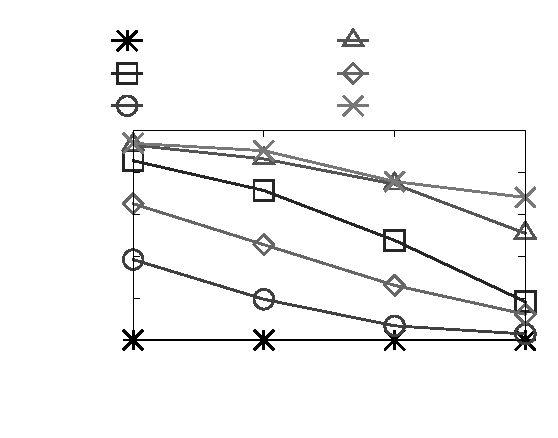
\includegraphics{phantomprimeprobe-declass}}%
    \gplfronttext
  \end{picture}%
\endgroup
}
\caption{\phantomCache\label{fig:phantom:jaccard:primeprobe:declass}}
\end{subfigure}%
\caption{Memory sharing disabled (\primeprobe attack),
  $\DCFn{}(\declassifyVar)\leftarrow\AIIFn{}(\cacheMap{})$ (or
  $\AIIFn{}(\phantomCacheMap{})$)}
\label{fig:defenseprimeprobe:declass}
\end{figure}

\begin{figure}
\begin{subfigure}[t]{0.495\linewidth}
\resizebox{\linewidth}{!}{\protect\small% GNUPLOT: LaTeX picture with Postscript
\begingroup
  \fontfamily{Times-Roman}%
  \selectfont
  \makeatletter
  \providecommand\color[2][]{%
    \GenericError{(gnuplot) \space\space\space\@spaces}{%
      Package color not loaded in conjunction with
      terminal option `colourtext'%
    }{See the gnuplot documentation for explanation.%
    }{Either use 'blacktext' in gnuplot or load the package
      color.sty in LaTeX.}%
    \renewcommand\color[2][]{}%
  }%
  \providecommand\includegraphics[2][]{%
    \GenericError{(gnuplot) \space\space\space\@spaces}{%
      Package graphicx or graphics not loaded%
    }{See the gnuplot documentation for explanation.%
    }{The gnuplot epslatex terminal needs graphicx.sty or graphics.sty.}%
    \renewcommand\includegraphics[2][]{}%
  }%
  \providecommand\rotatebox[2]{#2}%
  \@ifundefined{ifGPcolor}{%
    \newif\ifGPcolor
    \GPcolortrue
  }{}%
  \@ifundefined{ifGPblacktext}{%
    \newif\ifGPblacktext
    \GPblacktexttrue
  }{}%
  % define a \g@addto@macro without @ in the name:
  \let\gplgaddtomacro\g@addto@macro
  % define empty templates for all commands taking text:
  \gdef\gplbacktext{}%
  \gdef\gplfronttext{}%
  \makeatother
  \ifGPblacktext
    % no textcolor at all
    \def\colorrgb#1{}%
    \def\colorgray#1{}%
  \else
    % gray or color?
    \ifGPcolor
      \def\colorrgb#1{\color[rgb]{#1}}%
      \def\colorgray#1{\color[gray]{#1}}%
      \expandafter\def\csname LTw\endcsname{\color{white}}%
      \expandafter\def\csname LTb\endcsname{\color{black}}%
      \expandafter\def\csname LTa\endcsname{\color{black}}%
      \expandafter\def\csname LT0\endcsname{\color[rgb]{1,0,0}}%
      \expandafter\def\csname LT1\endcsname{\color[rgb]{0,1,0}}%
      \expandafter\def\csname LT2\endcsname{\color[rgb]{0,0,1}}%
      \expandafter\def\csname LT3\endcsname{\color[rgb]{1,0,1}}%
      \expandafter\def\csname LT4\endcsname{\color[rgb]{0,1,1}}%
      \expandafter\def\csname LT5\endcsname{\color[rgb]{1,1,0}}%
      \expandafter\def\csname LT6\endcsname{\color[rgb]{0,0,0}}%
      \expandafter\def\csname LT7\endcsname{\color[rgb]{1,0.3,0}}%
      \expandafter\def\csname LT8\endcsname{\color[rgb]{0.5,0.5,0.5}}%
    \else
      % gray
      \def\colorrgb#1{\color{black}}%
      \def\colorgray#1{\color[gray]{#1}}%
      \expandafter\def\csname LTw\endcsname{\color{white}}%
      \expandafter\def\csname LTb\endcsname{\color{black}}%
      \expandafter\def\csname LTa\endcsname{\color{black}}%
      \expandafter\def\csname LT0\endcsname{\color{black}}%
      \expandafter\def\csname LT1\endcsname{\color{black}}%
      \expandafter\def\csname LT2\endcsname{\color{black}}%
      \expandafter\def\csname LT3\endcsname{\color{black}}%
      \expandafter\def\csname LT4\endcsname{\color{black}}%
      \expandafter\def\csname LT5\endcsname{\color{black}}%
      \expandafter\def\csname LT6\endcsname{\color{black}}%
      \expandafter\def\csname LT7\endcsname{\color{black}}%
      \expandafter\def\csname LT8\endcsname{\color{black}}%
    \fi
  \fi
    \setlength{\unitlength}{0.0500bp}%
    \ifx\gptboxheight\undefined%
      \newlength{\gptboxheight}%
      \newlength{\gptboxwidth}%
      \newsavebox{\gptboxtext}%
    \fi%
    \setlength{\fboxrule}{0.5pt}%
    \setlength{\fboxsep}{1pt}%
\begin{picture}(5040.00,3888.00)%
    \gplgaddtomacro\gplbacktext{%
      \csname LTb\endcsname%%
      \put(962,780){\makebox(0,0)[r]{\strut{}$0$}}%
      \put(962,1183){\makebox(0,0)[r]{\strut{}$0.2$}}%
      \put(962,1586){\makebox(0,0)[r]{\strut{}$0.4$}}%
      \put(962,1989){\makebox(0,0)[r]{\strut{}$0.6$}}%
      \put(962,2392){\makebox(0,0)[r]{\strut{}$0.8$}}%
      \put(962,2795){\makebox(0,0)[r]{\strut{}$1$}}%
      \put(1118,520){\makebox(0,0){\strut{}$0$}}%
      \put(2373,520){\makebox(0,0){\strut{}$1$}}%
      \put(3628,520){\makebox(0,0){\strut{}$2$}}%
      \put(4883,520){\makebox(0,0){\strut{}$3$}}%
    }%
    \gplgaddtomacro\gplfronttext{%
      \csname LTb\endcsname%%
      \put(309,1787){\rotatebox{-270}{\makebox(0,0){\strut{}\JaccardWithDeclass{\secretsSetSize}}}}%
      \put(3000,182){\makebox(0,0){\strut{}$\log_2{\secretsSetSize}$}}%
      \csname LTb\endcsname%%
      \put(1365,3576){\makebox(0,0)[l]{\strut{}$\cachesetNmbr=1$}}%
      \csname LTb\endcsname%%
      \put(1365,3264){\makebox(0,0)[l]{\strut{}$\cachesetNmbr=2$}}%
      \csname LTb\endcsname%%
      \put(2832,3576){\makebox(0,0)[l]{\strut{}$\cachesetNmbr=4$}}%
      \csname LTb\endcsname%%
      \put(2832,3264){\makebox(0,0)[l]{\strut{}$\cachesetNmbr=8$}}%
      \csname LTb\endcsname%%
      \put(4299,3576){\makebox(0,0)[l]{\strut{}$\cachesetNmbr=16$}}%
    }%
    \gplbacktext
    \put(0,0){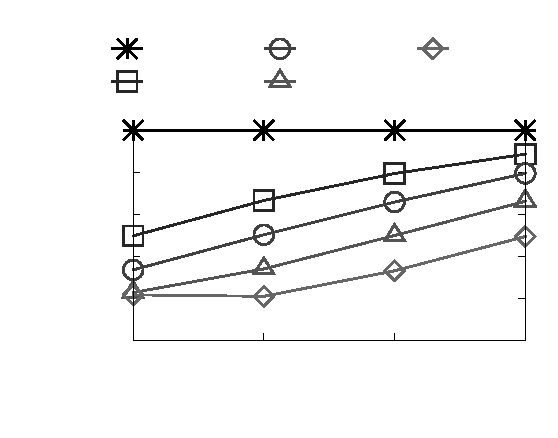
\includegraphics{scatterflushreload-declass}}%
    \gplfronttext
  \end{picture}%
\endgroup
}
\caption{\scatterCache\label{fig:scatter:jaccard:flushreload:declass}}
\end{subfigure}%
\centering
\begin{subfigure}[t]{0.495\linewidth}
\resizebox{\linewidth}{!}{\protect\small% GNUPLOT: LaTeX picture with Postscript
\begingroup
  \fontfamily{Times-Roman}%
  \selectfont
  \makeatletter
  \providecommand\color[2][]{%
    \GenericError{(gnuplot) \space\space\space\@spaces}{%
      Package color not loaded in conjunction with
      terminal option `colourtext'%
    }{See the gnuplot documentation for explanation.%
    }{Either use 'blacktext' in gnuplot or load the package
      color.sty in LaTeX.}%
    \renewcommand\color[2][]{}%
  }%
  \providecommand\includegraphics[2][]{%
    \GenericError{(gnuplot) \space\space\space\@spaces}{%
      Package graphicx or graphics not loaded%
    }{See the gnuplot documentation for explanation.%
    }{The gnuplot epslatex terminal needs graphicx.sty or graphics.sty.}%
    \renewcommand\includegraphics[2][]{}%
  }%
  \providecommand\rotatebox[2]{#2}%
  \@ifundefined{ifGPcolor}{%
    \newif\ifGPcolor
    \GPcolortrue
  }{}%
  \@ifundefined{ifGPblacktext}{%
    \newif\ifGPblacktext
    \GPblacktexttrue
  }{}%
  % define a \g@addto@macro without @ in the name:
  \let\gplgaddtomacro\g@addto@macro
  % define empty templates for all commands taking text:
  \gdef\gplbacktext{}%
  \gdef\gplfronttext{}%
  \makeatother
  \ifGPblacktext
    % no textcolor at all
    \def\colorrgb#1{}%
    \def\colorgray#1{}%
  \else
    % gray or color?
    \ifGPcolor
      \def\colorrgb#1{\color[rgb]{#1}}%
      \def\colorgray#1{\color[gray]{#1}}%
      \expandafter\def\csname LTw\endcsname{\color{white}}%
      \expandafter\def\csname LTb\endcsname{\color{black}}%
      \expandafter\def\csname LTa\endcsname{\color{black}}%
      \expandafter\def\csname LT0\endcsname{\color[rgb]{1,0,0}}%
      \expandafter\def\csname LT1\endcsname{\color[rgb]{0,1,0}}%
      \expandafter\def\csname LT2\endcsname{\color[rgb]{0,0,1}}%
      \expandafter\def\csname LT3\endcsname{\color[rgb]{1,0,1}}%
      \expandafter\def\csname LT4\endcsname{\color[rgb]{0,1,1}}%
      \expandafter\def\csname LT5\endcsname{\color[rgb]{1,1,0}}%
      \expandafter\def\csname LT6\endcsname{\color[rgb]{0,0,0}}%
      \expandafter\def\csname LT7\endcsname{\color[rgb]{1,0.3,0}}%
      \expandafter\def\csname LT8\endcsname{\color[rgb]{0.5,0.5,0.5}}%
    \else
      % gray
      \def\colorrgb#1{\color{black}}%
      \def\colorgray#1{\color[gray]{#1}}%
      \expandafter\def\csname LTw\endcsname{\color{white}}%
      \expandafter\def\csname LTb\endcsname{\color{black}}%
      \expandafter\def\csname LTa\endcsname{\color{black}}%
      \expandafter\def\csname LT0\endcsname{\color{black}}%
      \expandafter\def\csname LT1\endcsname{\color{black}}%
      \expandafter\def\csname LT2\endcsname{\color{black}}%
      \expandafter\def\csname LT3\endcsname{\color{black}}%
      \expandafter\def\csname LT4\endcsname{\color{black}}%
      \expandafter\def\csname LT5\endcsname{\color{black}}%
      \expandafter\def\csname LT6\endcsname{\color{black}}%
      \expandafter\def\csname LT7\endcsname{\color{black}}%
      \expandafter\def\csname LT8\endcsname{\color{black}}%
    \fi
  \fi
    \setlength{\unitlength}{0.0500bp}%
    \ifx\gptboxheight\undefined%
      \newlength{\gptboxheight}%
      \newlength{\gptboxwidth}%
      \newsavebox{\gptboxtext}%
    \fi%
    \setlength{\fboxrule}{0.5pt}%
    \setlength{\fboxsep}{1pt}%
\begin{picture}(5040.00,3888.00)%
    \gplgaddtomacro\gplbacktext{%
      \csname LTb\endcsname%%
      \put(962,780){\makebox(0,0)[r]{\strut{}$0$}}%
      \put(962,1183){\makebox(0,0)[r]{\strut{}$0.2$}}%
      \put(962,1586){\makebox(0,0)[r]{\strut{}$0.4$}}%
      \put(962,1989){\makebox(0,0)[r]{\strut{}$0.6$}}%
      \put(962,2392){\makebox(0,0)[r]{\strut{}$0.8$}}%
      \put(962,2795){\makebox(0,0)[r]{\strut{}$1$}}%
      \put(1118,520){\makebox(0,0){\strut{}$0$}}%
      \put(2373,520){\makebox(0,0){\strut{}$1$}}%
      \put(3628,520){\makebox(0,0){\strut{}$2$}}%
      \put(4883,520){\makebox(0,0){\strut{}$3$}}%
    }%
    \gplgaddtomacro\gplfronttext{%
      \csname LTb\endcsname%%
      \put(309,1787){\rotatebox{-270}{\makebox(0,0){\strut{}\JaccardWithDeclass{\secretsSetSize}}}}%
      \put(3000,182){\makebox(0,0){\strut{}$\log_2{\secretsSetSize}$}}%
      \csname LTb\endcsname%%
      \put(1365,3653){\makebox(0,0)[l]{\strut{}$\cachesetNmbr=1,\phantomR=1$}}%
      \csname LTb\endcsname%%
      \put(1365,3341){\makebox(0,0)[l]{\strut{}$\cachesetNmbr=4,\phantomR=1$}}%
      \csname LTb\endcsname%%
      \put(1365,3029){\makebox(0,0)[l]{\strut{}$\cachesetNmbr=4,\phantomR=2$}}%
      \csname LTb\endcsname%%
      \put(3534,3653){\makebox(0,0)[l]{\strut{}$\cachesetNmbr=8,\phantomR=1$}}%
      \csname LTb\endcsname%%
      \put(3534,3341){\makebox(0,0)[l]{\strut{}$\cachesetNmbr=8,\phantomR=2$}}%
      \csname LTb\endcsname%%
      \put(3534,3029){\makebox(0,0)[l]{\strut{}$\cachesetNmbr=16,\phantomR=1$}}%
    }%
    \gplbacktext
    \put(0,0){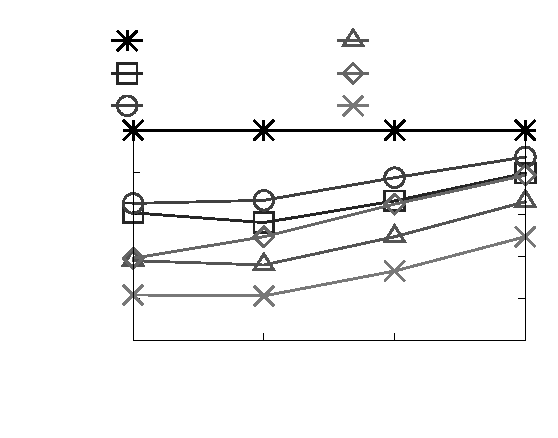
\includegraphics{phantomflushreload-declass}}%
    \gplfronttext
  \end{picture}%
\endgroup
}
\caption{\phantomCache\label{fig:phantom:jaccard:flushreload:declass} }
\end{subfigure}%
\caption{Memory sharing enabled (\flushreload attack),
$\DCFn{}(\declassifyVar)\leftarrow\AIIFn{}(\cacheMap{})$ (or $\AIIFn{}(\phantomCacheMap{})$) }
\end{figure}

When $\AIIFn{}(\cacheMap{})$ is unknown to the attacker, our previous
analysis shows that cache-based side channels are mitigated.  Werner
et al.~\cite{scatterCache} also discuss the possibility of this mapping
being disclosed to the attacker, however, through a profiling procedure.
If we declassify $\AIIFn{}(\cacheMap{})$, the interference
\JaccardWithDeclass{\secretsSetSize} will increase:
\figref{fig:scatter:jaccard:primeprobe:declass} shows
\JaccardWithDeclass{\secretsSetSize} due to \primeprobe attacks in
this case, and \figref{fig:scatter:jaccard:flushreload:declass} shows
the impact of this declassification on \flushreload attacks.

\if0
Declassifying the
$\DCFn{}(\textrm{`info'})\leftarrow\AIIFn{}(\cacheMap{})$ will help an
attacker to reverse engineer the possible domain of victim's memory address as only the
address shares the cache lines with the attacker's memory block cause
the cache contention. 
\fi

Similarly, using $\DCFn{}(\declassifyVar)\leftarrow
\AIIFn{}(\phantomCacheMap{\domainIdx})$, we evaluate \phantomCache's
leakage when the random mapping is declassified; results are shown in
\figref{fig:phantom:jaccard:primeprobe:declass} and
\figref{fig:phantom:jaccard:flushreload:declass}.  Comparing
\figref{fig:phantom:jaccard:primeprobe:declass} and
\figref{fig:scatter:jaccard:primeprobe:declass}, \phantomCache's
leakage (measured by \JaccardWithDeclass{\secretsSetSize}) for
unshared memory is higher than \scatterCache's when $\phantomR=1$. The
strength of \phantomCache is revealed when \phantomR increases, since
it allows memory blocks to map to more than one cache set.
Specifically, the leakage for \scatterCache's `$\cachesetNmbr=4$' is
much less than \phantomCache's `$\cachesetNmbr=4$, $\phantomR=1$' but
is similar to \phantomCache's `$\cachesetNmbr=4$,
$\phantomR=2$'. However, \phantomCache with $\phantomR=2$ provides
weaker protection for \flushreload than \phantomCache with
$\phantomR=1$ and \scatterCache.


\subsection{Leaking exponent in modular exponentiation}
\label{dinome:sec:exp:modexp}

\begin{figure}
\begin{subfigure}[b]{0.47\columnwidth}
\begin{algorithmic}[1]
\footnotesize{
\Function{modexp}{\plaintext{},\privK{}}
\State $\encrypted \leftarrow 1$
\if0
\State $\precomputedPlaintext{2} \leftarrow \plaintext{}\times\plaintext{}\bmod\modulus$
\For{$\modexpRound \leftarrow 1 \text{ to } 2^{\window-1}-1$}
\State $\precomputedPlaintext{2\modexpRound+1} \leftarrow$
\Statex \hfill$\precomputedPlaintext{2\modexpRound-1}\times\precomputedPlaintext{2}\bmod\modulus$
\EndFor
\fi
\For {$\modexpRound \leftarrow n$ \text{ to } 1} \label{line:round:start}
\State $\encrypted\leftarrow \encrypted\times\encrypted \bmod\modulus$
\If{$\privK{\modexpRound}\neq 0$} \label{line:beqz}
\State $\encrypted\leftarrow\encrypted \times\precomputedPlaintext{\privK{\modexpRound}}$
\EndIf
\EndFor\\\label{line:round:end}
\Return \encrypted
\EndFunction
}
\end{algorithmic}
\vspace{4ex}
\caption{Algorithm \label{fig:alg:modexp}}
\end{subfigure}%
\hfill
\begin{subfigure}[b]{0.47\linewidth}
\centering
\if 0
\footnotesize{
\begin{tabbing}
** \= ** \= ** \= \kill
\>	li sp, 0x80000000\\
\>	li  a0,1 \\
\>	li a2, \modulus \\
\>	li a3, $\SecFn{}(\privK{\modexpRound})$\\
.OneIteration:\\
\>	mulw	a0,a0,a0\\
\>	sll	a5,a3,2\\
\>	add	a5,sp,a5\\
\>	remw	a0,a0,a2\\
\>	beqz	a3,.NextIteration\\
\>	lw	a5,0(a5)\\
\>	mulw	a0,a0,a5\\
\>	remw	a0,a0,a2\\
.NextIteration:\\
\end{tabbing}
}
\fi
\lstset{language=[riscv]Assembler,style=customriscv,escapechar=|}
\centering
\begin{lstlisting}
|$\proc(\ACIFn{}, \AIIFn{}, \SecFn{})$|
  li sp, 0x80000400    
  li  a0,1     
  li a2, |\modulus|
  li a3, |$\SecFn{}(\privK{\modexpRound})$|   
.oneIteration:    
  mulw  a0,a0,a0      
  remw  a0,a0,a2    
  beqz  a3,.NextIteration   
  sll  a5,a3,2    
  add  a5,sp,a5   
  lw  a5,0(a5)    
  mulw  a0,a0,a5    
  remw  a0,a0,a2
.NextIteration: 
\end{lstlisting}
\vspace{-1ex}
\caption{Assembly for one iteration}
\label{code:assembly:modexp}
\end{subfigure}%
\if0
\begin{subfigure}{0.3\linewidth}
\footnotesize{
\begin{tabbing}
** \= ** \= ** \= \kill
\proc(\ACIFn{},  \AIIFn{}, \SecFn{}) \\
\> multiply \encrypted with \encrypted\\
\> \encrypted modulo \modulus\\ 
\> \addr{} $\leftarrow$ $\plaintext{0}$.addr+$\SecFn{}(\privK_{i})\ll 2$ \\
\> if $\SecFn{}(\privK_{i})\neq0$\\
\>\> if \cachemiss(\HwFn{}{\cycle}(\meta), \addr)\\
\>\>\> fill \addr to  \HwFn{}{\nextCycle}(\meta)\\
\>\>\> fill  \HwFn{}{\nextNextCycle}(`cachedata') from memory\\
\>\>load $\plaintext{\privK_{i}}$ at \addr from cache\\ 
\> ...
\end{tabbing}
}
\caption{\proc logic snippet\label{fig:pseudo:modexp}}
\end{subfigure}%
\fi
\caption[Sliding window modular exponentiation with window size
  \window]{Sliding window modular exponentiation with window size
  \window.  $\privK{n} \ldots \privK{1}$ is the private key \privK{} where
  each $\privK{\modexpRound}$ ($\modexpRound=1, \ldots, n$) is a
  \window-bit value.}
\label{fig:code:modexp}
\end{figure}

The evaluations in \secref{dinome:sec:exp:cache} and
\secref{dinome:sec:exp:cachedefense} focused on whether the adversary could
detect the victim's access to a particular memory block, which is a
well-known vector of information leakage.  To further demonstrate the
utility of our framework in measuring this type of leakage, here we
consider a classic example whereby the secret is not a memory address,
but rather is a cryptographic secret that, due to the algorithm in
use, can influence the victim's cache footprint.

The particular example we evaluate here is modular exponentiation as
used in algorithms such as RSA.  A textbook implementation of modular
exponentiation uses a sliding-window method that is known to leak
information in caches~\cite{zhang2012cross,bernstein2017sliding}.  As
shown in \figref{fig:alg:modexp}, the algorithm leverages some small
powers \precomputedPlaintext{\powerIdx} of a base \plaintext{} (where
$\powerIdx< 2^{\window}-1$) to compute a larger power.  Accesses to
those precomputed powers is determined by the window-sized segment
\privK{\modexpRound} of the private key \privK{} in each loop
iteration \modexpRound.  First, this procedure will leak via the cache
whether \privK{\modexpRound} is zero.  Second, since the precomputed
elements are addressed by \privK{\modexpRound}, an attacker may
identify up to $\log_2 \cachesetNmbr$ bits about
$\privK{\modexpRound}$ if those precomputed powers map to different
cache sets.  \if0
Besides,  the window-sized segment
\privK{\modexpRound} is not an arbitrary \window-bit value where
\window is the sliding-window size; instead, it is either zero or a
odd value.  
\mkr{Are you sure that's true?  I'm not sure I've ever
thought about that before ...}\zz{I got this from Sec 2.2 in
\cite{bernstein2017sliding}.
$\privK{}=\sum_{\modexpRound}^{n-1}\privK{\modexpRound}*
2^{\modexpRound}$ where \privK{\modexpRound} is either 0 or an odd
number between 1 and $2^\window$.}  \zz{ I think this assumption is
used to reduce the number of loops but is not that necessary
to make the above algorithm true. I should remove this assumption as my
current evaluation does not constrain \privK{\modexpRound}}That is, the
lowest bit is surely leaked no matter the window size choice.
\fi

To evaluate the one-round leakage of \figref{fig:alg:modexp}, we used
the RISC-V assembly shown in \figref{code:assembly:modexp} in \boom
with a 2-way, 8-set cache ($\cachesetNmbr=8$). The
\JaccardRand{\secretsSetSize} measure shown in
\figref{fig:modexp:jaccard:sym} indicates that the amount of leakage
for one loop iteration \modexpRound is limited, when $\window\le4$ and
so the precomputed \plaintext{} only uses up to $4 \times 2^4=64$ bytes
(i.e., one cache line).  When $4<\window<8$, the side channel will
leak more about $\privK{\modexpRound}$ when \window increases. Thus,
choosing $\window=4$ is the best choice to protect the secret in our
cache configuration.

To further diagnose the cause of leakage, we generated the interference
rules for $\window=1$, $\window=4$, and $\window=8$. When $\window=1$,
we obtain a single rule with precision and recall of 1.0, namely
\[
\ACIFn{}(\loadVar)[0]\ge 1 \wedge \ACIFn{}(\loadVar)[8]\ge1
\]
This has no \SecFn{} or \SecFnAlt{} related conjuncts, indicating that
the 1-bit secret $\privK{\modexpRound}$ is fully leaked when an
attacker \Prime{s} one cache set.  In contrast, when $\window=4$, the
top rules (precision of 1.0, recall $\ge 0.5$) include some \SecFn{}
or \SecFnAlt{} related conjuncts, constraining the secret value to be
zero, e.g.,
\[
\SecFn{}(\privK{\modexpRound}) <1
\wedge \ACIFn{}(\loadVar)[0]\ge 1 \wedge \ACIFn{}(\loadVar)[8]\ge
1
\]
That is, it only leaks whether it is zero or not for a 4-bit secret.

When $\window>4$, however, the most important cause of leakage changes
from whether a memory access happens to which cache set is used by
\privK{\modexpRound}. For example, when $\window=8$, one highly ranked
rule (precision of 1.0, recall $\ge 0.04$) is
\begin{align*}
\begin{array}{@{}r@{\hspace{0.25em}}r@{\hspace{0.25em}}r@{\hspace{0.25em}}r@{\hspace{0.25em}}r@{\hspace{0.25em}}r}
& \SecFnAlt{}(\privK{\modexpRound})[6]< 1 & \wedge
& \SecFnAlt{}(\privK{\modexpRound})[5]\ge 1 & \wedge
& \SecFnAlt{}(\privK{\modexpRound})[4]< 1\\
  \wedge & \SecFn{}(\privK{\modexpRound})[4]\ge 1 & \wedge & \ACIFn{}(\loadVar)[10]\ge 1 & \wedge & \ACIFn{}(\loadVar)[2]\ge 1
\end{array}
%\label{eqn:modexp8-interference-rule}
\end{align*}
which indicates that the attacker can distinguish an
$\SecFnAlt{}(\privK{\modexpRound})$ with
$\SecFnAlt{}(\privK{\modexpRound})[4:6]=2$ from an
$\SecFn{}(\privK{\modexpRound})$ with
$\SecFn{}(\privK{\modexpRound})[4:6] \in \{1,3,5,7\}$ if the attacker
\Prime{s} cache set 2. Similar to the analysis in
\secref{dinome:sec:exp:cache:normal:unshared}, rules for $\window=8$
illustrate that an attacker can reveal the cache set used by the
victim (e.g., secret bits 4-6) when priming all cache sets.

\if0
to the BOOM's instructions buffer and allow the CPU running it for 100
cycles. Then our framework will generate a formula
\HwPostcondition{\proc}{100}(\ACIFn{}, \AIIFn{}, \SecFn{}, \HwFn{}{})
encoding the software and hardware combined logic(the pseudo logic is
described in \figref{fig:pseudo:modexp}) among your
$\AIIFn{\proc}(\plaintext),\SecFn{\proc}(\privK),\HwFn{\proc}{0}(\meta),
\HwFn{}{100}(\meta)$. 
\fi

\begin{figure}
\begin{subfigure}{0.495\linewidth}
\resizebox{\linewidth}{!}{\protect\small% GNUPLOT: LaTeX picture with Postscript
\begingroup
  \fontfamily{Times-Roman}%
  \selectfont
  \makeatletter
  \providecommand\color[2][]{%
    \GenericError{(gnuplot) \space\space\space\@spaces}{%
      Package color not loaded in conjunction with
      terminal option `colourtext'%
    }{See the gnuplot documentation for explanation.%
    }{Either use 'blacktext' in gnuplot or load the package
      color.sty in LaTeX.}%
    \renewcommand\color[2][]{}%
  }%
  \providecommand\includegraphics[2][]{%
    \GenericError{(gnuplot) \space\space\space\@spaces}{%
      Package graphicx or graphics not loaded%
    }{See the gnuplot documentation for explanation.%
    }{The gnuplot epslatex terminal needs graphicx.sty or graphics.sty.}%
    \renewcommand\includegraphics[2][]{}%
  }%
  \providecommand\rotatebox[2]{#2}%
  \@ifundefined{ifGPcolor}{%
    \newif\ifGPcolor
    \GPcolortrue
  }{}%
  \@ifundefined{ifGPblacktext}{%
    \newif\ifGPblacktext
    \GPblacktexttrue
  }{}%
  % define a \g@addto@macro without @ in the name:
  \let\gplgaddtomacro\g@addto@macro
  % define empty templates for all commands taking text:
  \gdef\gplbacktext{}%
  \gdef\gplfronttext{}%
  \makeatother
  \ifGPblacktext
    % no textcolor at all
    \def\colorrgb#1{}%
    \def\colorgray#1{}%
  \else
    % gray or color?
    \ifGPcolor
      \def\colorrgb#1{\color[rgb]{#1}}%
      \def\colorgray#1{\color[gray]{#1}}%
      \expandafter\def\csname LTw\endcsname{\color{white}}%
      \expandafter\def\csname LTb\endcsname{\color{black}}%
      \expandafter\def\csname LTa\endcsname{\color{black}}%
      \expandafter\def\csname LT0\endcsname{\color[rgb]{1,0,0}}%
      \expandafter\def\csname LT1\endcsname{\color[rgb]{0,1,0}}%
      \expandafter\def\csname LT2\endcsname{\color[rgb]{0,0,1}}%
      \expandafter\def\csname LT3\endcsname{\color[rgb]{1,0,1}}%
      \expandafter\def\csname LT4\endcsname{\color[rgb]{0,1,1}}%
      \expandafter\def\csname LT5\endcsname{\color[rgb]{1,1,0}}%
      \expandafter\def\csname LT6\endcsname{\color[rgb]{0,0,0}}%
      \expandafter\def\csname LT7\endcsname{\color[rgb]{1,0.3,0}}%
      \expandafter\def\csname LT8\endcsname{\color[rgb]{0.5,0.5,0.5}}%
    \else
      % gray
      \def\colorrgb#1{\color{black}}%
      \def\colorgray#1{\color[gray]{#1}}%
      \expandafter\def\csname LTw\endcsname{\color{white}}%
      \expandafter\def\csname LTb\endcsname{\color{black}}%
      \expandafter\def\csname LTa\endcsname{\color{black}}%
      \expandafter\def\csname LT0\endcsname{\color{black}}%
      \expandafter\def\csname LT1\endcsname{\color{black}}%
      \expandafter\def\csname LT2\endcsname{\color{black}}%
      \expandafter\def\csname LT3\endcsname{\color{black}}%
      \expandafter\def\csname LT4\endcsname{\color{black}}%
      \expandafter\def\csname LT5\endcsname{\color{black}}%
      \expandafter\def\csname LT6\endcsname{\color{black}}%
      \expandafter\def\csname LT7\endcsname{\color{black}}%
      \expandafter\def\csname LT8\endcsname{\color{black}}%
    \fi
  \fi
    \setlength{\unitlength}{0.0500bp}%
    \ifx\gptboxheight\undefined%
      \newlength{\gptboxheight}%
      \newlength{\gptboxwidth}%
      \newsavebox{\gptboxtext}%
    \fi%
    \setlength{\fboxrule}{0.5pt}%
    \setlength{\fboxsep}{1pt}%
\begin{picture}(5040.00,3600.00)%
    \gplgaddtomacro\gplbacktext{%
      \csname LTb\endcsname%
      \put(695,660){\makebox(0,0)[r]{\strut{}$0$}}%
      \put(695,1195){\makebox(0,0)[r]{\strut{}$0.2$}}%
      \put(695,1730){\makebox(0,0)[r]{\strut{}$0.4$}}%
      \put(695,2265){\makebox(0,0)[r]{\strut{}$0.6$}}%
      \put(695,2800){\makebox(0,0)[r]{\strut{}$0.8$}}%
      \put(695,3335){\makebox(0,0)[r]{\strut{}$1$}}%
      \put(827,440){\makebox(0,0){\strut{}$0$}}%
      \put(1410,440){\makebox(0,0){\strut{}$1$}}%
      \put(1993,440){\makebox(0,0){\strut{}$2$}}%
      \put(2576,440){\makebox(0,0){\strut{}$3$}}%
      \put(3158,440){\makebox(0,0){\strut{}$4$}}%
      \put(3741,440){\makebox(0,0){\strut{}$5$}}%
      \put(4324,440){\makebox(0,0){\strut{}$6$}}%
      \put(4907,440){\makebox(0,0){\strut{}$7$}}%
    }%
    \gplgaddtomacro\gplfronttext{%
      \csname LTb\endcsname%
      \put(176,1997){\rotatebox{-270}{\makebox(0,0){\strut{}\JaccardRand{\secretsSetSize}}}}%
      \put(2867,154){\makebox(0,0){\strut{}$\log_2{\secretsSetSize}$}}%
      \csname LTb\endcsname%
      \put(2626,3190){\makebox(0,0)[l]{\strut{}$\window=1$}}%
      \csname LTb\endcsname%
      \put(2626,2948){\makebox(0,0)[l]{\strut{}$\window=2$}}%
      \csname LTb\endcsname%
      \put(2626,2706){\makebox(0,0)[l]{\strut{}$\window=3$}}%
      \csname LTb\endcsname%
      \put(2626,2464){\makebox(0,0)[l]{\strut{}$\window=4$}}%
      \csname LTb\endcsname%
      \put(3982,3190){\makebox(0,0)[l]{\strut{}$\window=5$}}%
      \csname LTb\endcsname%
      \put(3982,2948){\makebox(0,0)[l]{\strut{}$\window=6$}}%
      \csname LTb\endcsname%
      \put(3982,2706){\makebox(0,0)[l]{\strut{}$\window=7$}}%
      \csname LTb\endcsname%
      \put(3982,2464){\makebox(0,0)[l]{\strut{}$\window=8$}}%
    }%
    \gplbacktext
    \put(0,0){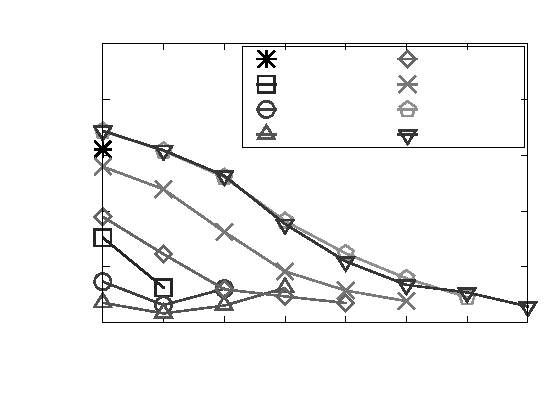
\includegraphics{modexp_sym}}%
    \gplfronttext
  \end{picture}%
\endgroup
}
\caption{Symbolic $\ACIFn{}(\loadVar)$}
\label{fig:modexp:jaccard:sym}
\end{subfigure}%
\begin{subfigure}{0.495\linewidth}
\resizebox{\linewidth}{!}{\protect\small% GNUPLOT: LaTeX picture with Postscript
\begingroup
  \fontfamily{Times-Roman}%
  \selectfont
  \makeatletter
  \providecommand\color[2][]{%
    \GenericError{(gnuplot) \space\space\space\@spaces}{%
      Package color not loaded in conjunction with
      terminal option `colourtext'%
    }{See the gnuplot documentation for explanation.%
    }{Either use 'blacktext' in gnuplot or load the package
      color.sty in LaTeX.}%
    \renewcommand\color[2][]{}%
  }%
  \providecommand\includegraphics[2][]{%
    \GenericError{(gnuplot) \space\space\space\@spaces}{%
      Package graphicx or graphics not loaded%
    }{See the gnuplot documentation for explanation.%
    }{The gnuplot epslatex terminal needs graphicx.sty or graphics.sty.}%
    \renewcommand\includegraphics[2][]{}%
  }%
  \providecommand\rotatebox[2]{#2}%
  \@ifundefined{ifGPcolor}{%
    \newif\ifGPcolor
    \GPcolortrue
  }{}%
  \@ifundefined{ifGPblacktext}{%
    \newif\ifGPblacktext
    \GPblacktexttrue
  }{}%
  % define a \g@addto@macro without @ in the name:
  \let\gplgaddtomacro\g@addto@macro
  % define empty templates for all commands taking text:
  \gdef\gplbacktext{}%
  \gdef\gplfronttext{}%
  \makeatother
  \ifGPblacktext
    % no textcolor at all
    \def\colorrgb#1{}%
    \def\colorgray#1{}%
  \else
    % gray or color?
    \ifGPcolor
      \def\colorrgb#1{\color[rgb]{#1}}%
      \def\colorgray#1{\color[gray]{#1}}%
      \expandafter\def\csname LTw\endcsname{\color{white}}%
      \expandafter\def\csname LTb\endcsname{\color{black}}%
      \expandafter\def\csname LTa\endcsname{\color{black}}%
      \expandafter\def\csname LT0\endcsname{\color[rgb]{1,0,0}}%
      \expandafter\def\csname LT1\endcsname{\color[rgb]{0,1,0}}%
      \expandafter\def\csname LT2\endcsname{\color[rgb]{0,0,1}}%
      \expandafter\def\csname LT3\endcsname{\color[rgb]{1,0,1}}%
      \expandafter\def\csname LT4\endcsname{\color[rgb]{0,1,1}}%
      \expandafter\def\csname LT5\endcsname{\color[rgb]{1,1,0}}%
      \expandafter\def\csname LT6\endcsname{\color[rgb]{0,0,0}}%
      \expandafter\def\csname LT7\endcsname{\color[rgb]{1,0.3,0}}%
      \expandafter\def\csname LT8\endcsname{\color[rgb]{0.5,0.5,0.5}}%
    \else
      % gray
      \def\colorrgb#1{\color{black}}%
      \def\colorgray#1{\color[gray]{#1}}%
      \expandafter\def\csname LTw\endcsname{\color{white}}%
      \expandafter\def\csname LTb\endcsname{\color{black}}%
      \expandafter\def\csname LTa\endcsname{\color{black}}%
      \expandafter\def\csname LT0\endcsname{\color{black}}%
      \expandafter\def\csname LT1\endcsname{\color{black}}%
      \expandafter\def\csname LT2\endcsname{\color{black}}%
      \expandafter\def\csname LT3\endcsname{\color{black}}%
      \expandafter\def\csname LT4\endcsname{\color{black}}%
      \expandafter\def\csname LT5\endcsname{\color{black}}%
      \expandafter\def\csname LT6\endcsname{\color{black}}%
      \expandafter\def\csname LT7\endcsname{\color{black}}%
      \expandafter\def\csname LT8\endcsname{\color{black}}%
    \fi
  \fi
    \setlength{\unitlength}{0.0500bp}%
    \ifx\gptboxheight\undefined%
      \newlength{\gptboxheight}%
      \newlength{\gptboxwidth}%
      \newsavebox{\gptboxtext}%
    \fi%
    \setlength{\fboxrule}{0.5pt}%
    \setlength{\fboxsep}{1pt}%
\begin{picture}(5040.00,3600.00)%
    \gplgaddtomacro\gplbacktext{%
      \csname LTb\endcsname%
      \put(695,660){\makebox(0,0)[r]{\strut{}$0$}}%
      \put(695,1195){\makebox(0,0)[r]{\strut{}$0.2$}}%
      \put(695,1730){\makebox(0,0)[r]{\strut{}$0.4$}}%
      \put(695,2265){\makebox(0,0)[r]{\strut{}$0.6$}}%
      \put(695,2800){\makebox(0,0)[r]{\strut{}$0.8$}}%
      \put(695,3335){\makebox(0,0)[r]{\strut{}$1$}}%
      \put(827,440){\makebox(0,0){\strut{}$0$}}%
      \put(1410,440){\makebox(0,0){\strut{}$1$}}%
      \put(1993,440){\makebox(0,0){\strut{}$2$}}%
      \put(2576,440){\makebox(0,0){\strut{}$3$}}%
      \put(3158,440){\makebox(0,0){\strut{}$4$}}%
      \put(3741,440){\makebox(0,0){\strut{}$5$}}%
      \put(4324,440){\makebox(0,0){\strut{}$6$}}%
      \put(4907,440){\makebox(0,0){\strut{}$7$}}%
    }%
    \gplgaddtomacro\gplfronttext{%
      \csname LTb\endcsname%
      \put(176,1997){\rotatebox{-270}{\makebox(0,0){\strut{}\JaccardRand{\secretsSetSize}}}}%
      \put(2867,154){\makebox(0,0){\strut{}$\log_2{\secretsSetSize}$}}%
      \csname LTb\endcsname%
      \put(2626,3190){\makebox(0,0)[l]{\strut{}$\window=1$}}%
      \csname LTb\endcsname%
      \put(2626,2948){\makebox(0,0)[l]{\strut{}$\window=2$}}%
      \csname LTb\endcsname%
      \put(2626,2706){\makebox(0,0)[l]{\strut{}$\window=3$}}%
      \csname LTb\endcsname%
      \put(2626,2464){\makebox(0,0)[l]{\strut{}$\window=4$}}%
      \csname LTb\endcsname%
      \put(3982,3190){\makebox(0,0)[l]{\strut{}$\window=5$}}%
      \csname LTb\endcsname%
      \put(3982,2948){\makebox(0,0)[l]{\strut{}$\window=6$}}%
      \csname LTb\endcsname%
      \put(3982,2706){\makebox(0,0)[l]{\strut{}$\window=7$}}%
      \csname LTb\endcsname%
      \put(3982,2464){\makebox(0,0)[l]{\strut{}$\window=8$}}%
    }%
    \gplbacktext
    \put(0,0){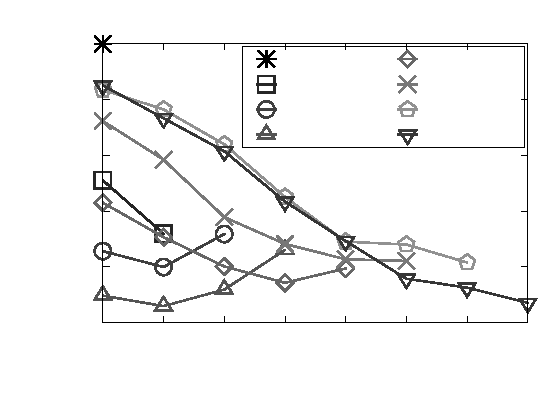
\includegraphics{modexp_primeprobe}}%
    \gplfronttext
  \end{picture}%
\endgroup
}
\caption{$\forall \blockIdx: \ACIFn{}(\loadVar)[\blockIdx] = 1$}
\label{fig:modexp:jaccard:prime}
\end{subfigure}%
\caption{\JaccardRand{\secretsSetSize} for \textsc{Modexp} in 2-way, 8-set cache}
\end{figure}

\iffalse
\begin{table}
{\scriptsize
\caption{Interference decision rules for modexp}
\label{tab:modexp:rule}
\begin{tabular}{m{\colW}m{\colR}m{\colRule-\colW}m{\colPrecision}m{\colRecall}}
\toprule
\window && Interference rule (\interferenceRule{}) & Precision & Recall \\
\midrule
1&$\interferenceRule{0}$&$\ACIFn{}(\loadVar)[0]\ge 1 \wedge
\ACIFn{}(\loadVar)[8]\ge1$&1.00&1.00\\
\hline
\multirow{2}{*}{4}&$\interferenceRule{0}$&$\SecFn{}(\privK{\modexpRound}) <1
\wedge \ACIFn{}(\loadVar)[0]\ge 1 \wedge \ACIFn{}(\loadVar)[8]\ge
1$&1.00&0.50\\
& $\interferenceRule{1}$&$ \SecFnAlt{}(\privK{\modexpRound})<1 \wedge
\ACIFn{}(\loadVar)[0]\ge 1 \wedge \ACIFn{}(\loadVar)[8]\ge 1$&1.00&0.53\\
\hline
\multirow{3}{*}{8} &
$\interferenceRule{0}$&$\SecFn{}(\privK{\modexpRound})[4]\ge 1 \wedge \SecFnAlt{}(\privK{\modexpRound})[6]< 1 \wedge \SecFnAlt{}(\privK{\modexpRound})[5]\ge 1 \wedge \SecFnAlt{}(\privK{\modexpRound})[4]< 1 \wedge \ACIFn{}(\loadVar)[10]\ge 1 \wedge \ACIFn{}(\loadVar)[2]\ge 1$&1.00&0.04\\
&$\interferenceRule{1}$&$\SecFn{}(\privK{\modexpRound})[6]\ge 1 \wedge \SecFn{}(\privK{\modexpRound})[6]< 1 \wedge \SecFn{}(\privK{\modexpRound})[5]< 1 \wedge \SecFn{}(\privK{\modexpRound})[4]\ge 1 \wedge \ACIFn{}(\loadVar)[9]\ge 1 \wedge \ACIFn{}(\loadVar)[1]\ge 1$&1.00&0.04\\
&$\interferenceRule{2}$&$\SecFn{}(\privK{\modexpRound})[6]\ge 1 \wedge \SecFnAlt{}(\privK{\modexpRound})[6]< 1 \wedge \SecFnAlt{}(\privK{\modexpRound})[5]\ge 1 \wedge \SecFnAlt{}(\privK{\modexpRound})[4]\ge 1 \wedge \ACIFn{}(\loadVar)[11]\ge 1 \wedge \ACIFn{}(\loadVar)[3]\ge 1$&1.00&0.04\\
\bottomrule
\end{tabular}
}
\end{table}
\fi

\if0
\begin{table}
{\scriptsize
\caption{Interference decision rules for modexp ($\window=1$)}
\label{table:modexp:rule:1}
\begin{tabular}{m{\colR}m{\colRule}m{\colPrecision}m{\colRecall}}
\toprule
 & Interference rule (\interferenceRule{}) & Precision & Recall \\
\midrule
$\interferenceRule{0}$&$\ACIFn{}(\loadVar)[0]\ge 1 \wedge
\ACIFn{}(\loadVar)[8]\ge1$&1.00&1.00\\
\bottomrule
\end{tabular}
}
\end{table}
\begin{table}
\begingroup
\everymath{\scriptstyle}
\footnotesize{
\caption{Interference decision rules for modexp ($\window=4$)}
\label{table:cache:morerule}
$\linearFeature{0}=0.555208\SecFn{}(\secretVar)+0.444792\SecFnAlt{}(\secretVar)$\\
\begin{tabular}{m{\colR}m{\colRule}m{\colPrecision}m{\colRecall}}
\toprule
 &Interference rule (\interferenceRule{}) & Precision & Recall \\
\midrule
$\interferenceRule{0}$&$  \SecFn{}(\secretVar) <1 \wedge \ACIFn{}(\loadVar)[0]\ge 1 \wedge \ACIFn{}(\loadVar)[8]\ge 1$&1.00&0.50\\
$\interferenceRule{1}$&$ \SecFnAlt{}(\secretVar)<1 \wedge
\ACIFn{}(\loadVar)[0]\ge 1 \wedge \ACIFn{}(\loadVar)[8]\ge 1$&1.00&0.53\\
$\interferenceRule{2}$&$\linearFeature{0}<7 \wedge
\ACIFn{}(\loadVar)[8]\ge 1 \wedge \ACIFn{}(\loadVar)[0]\ge 1$&0.91&0.90\\
$\interferenceRule{3}$&$  \SecFn{}(\secretVar) <1$&0.91&0.50\\
$\interferenceRule{4}$&$\linearFeature{0}<9 \wedge \ACIFn{}(\loadVar)[8]\ge 1 \wedge \ACIFn{}(\loadVar)[0]\ge 1$&0.87&1.00\\
\bottomrule
\end{tabular}
}
\endgroup
\end{table}
\begin{table}
\begingroup
\everymath{\scriptstyle}
\footnotesize{
\caption{Selected interference decision rules for modexp ($\window=8$)}
\label{table:cache:morerule}
\begin{tabular}{m{\colR}m{\colRule}m{\colPrecision}m{\colRecall}}
\toprule
 &Interference rule (\interferenceRule{}) & Precision & Recall \\
\midrule
$\interferenceRule{0}$&$\SecFn{}(\privK{\modexpRound})[4]\ge 1 \wedge \SecFnAlt{}(\privK{\modexpRound})[6]< 1 \wedge \SecFnAlt{}(\privK{\modexpRound})[5]\ge 1 \wedge \SecFnAlt{}(\privK{\modexpRound})[4]< 1 \wedge \ACIFn{}(\loadVar)[10]\ge 1 \wedge \ACIFn{}(\loadVar)[2]\ge 1$&1.00&0.04\\
$\interferenceRule{1}$&$\diffFeature{6}\ge 1 \wedge \SecFn{}(\privK{\modexpRound})[6]< 1 \wedge \SecFn{}(\privK{\modexpRound})[5]< 1 \wedge \SecFn{}(\privK{\modexpRound})[4]\ge 1 \wedge \ACIFn{}(\loadVar)[9]\ge 1 \wedge \ACIFn{}(\loadVar)[1]\ge 1$&1.00&0.04\\
$\interferenceRule{2}$&$\SecFn{}(\privK{\modexpRound})[6]\ge 1 \wedge \SecFnAlt{}(\privK{\modexpRound})[6]< 1 \wedge \SecFnAlt{}(\privK{\modexpRound})[5]\ge 1 \wedge \SecFnAlt{}(\privK{\modexpRound})[4]\ge 1 \wedge \ACIFn{}(\loadVar)[11]\ge 1 \wedge \ACIFn{}(\loadVar)[3]\ge 1$&1.00&0.04\\
$\interferenceRule{3}$&$\diffFeature{6}\ge 1 \wedge \SecFn{}(\privK{\modexpRound})[6]\ge 1 \wedge \SecFn{}(\privK{\modexpRound})[5]\ge 1 \wedge \SecFn{}(\privK{\modexpRound})[4]\ge 1 \wedge \ACIFn{}[31]\ge 1 \wedge \ACIFn{}[23]\ge 1$&1.00&0.04\\
$\interferenceRule{4}$&$\SecFn{}(\privK{\modexpRound})[5]< 1 \wedge \SecFnAlt{}(\privK{\modexpRound})[6]< 1 \wedge \SecFnAlt{}(\privK{\modexpRound})[5]\ge 1 \wedge \SecFnAlt{}(\privK{\modexpRound})[4]< 1 \wedge \ACIFn{}(\loadVar)[10]\ge 1 \wedge \ACIFn{}(\loadVar)[2]\ge 1$&1.00&0.04\\
$\interferenceRule{5}$&$\SecFn{}(\privK{\modexpRound})[6]\ge 1 \wedge \SecFnAlt{}(\privK{\modexpRound})[6]< 1 \wedge \SecFnAlt{}(\privK{\modexpRound})[5]\ge 1 \wedge \SecFnAlt{}(\privK{\modexpRound})[4]< 1 \wedge \ACIFn{}(\loadVar)[10]\ge 1 \wedge \ACIFn{}(\loadVar)[2]\ge 1$&1.00&0.04\\
$\interferenceRule{6}$&$\SecFn{}(\privK{\modexpRound})[6]< 1 \wedge \SecFn{}(\privK{\modexpRound})[5]\ge 1 \wedge \SecFn{}(\privK{\modexpRound})[4]< 1 \wedge \SecFnAlt{}(\privK{\modexpRound})[4]\ge 1 \wedge \ACIFn{}(\loadVar)[10]\ge 1 \wedge \ACIFn{}(\loadVar)[2]\ge 1$&1.00&0.04\\
$\interferenceRule{7}$&$\diffFeature[4]\ge 1 \wedge \SecFn{}(\privK{\modexpRound})[6]< 1 \wedge \SecFn{}(\privK{\modexpRound})[5]\ge 1 \wedge \SecFn{}(\privK{\modexpRound})[4]< 1 \wedge \ACIFn{}(\loadVar)[10]\ge 1 \wedge \ACIFn{}(\loadVar)[2]\ge 1$&1.00&0.04\\
$\interferenceRule{8}$&$\diffFeature{6}\ge 1 \wedge \SecFn{}(\privK{\modexpRound})[6]\ge 1 \wedge \SecFn{}(\privK{\modexpRound})[5]< 1 \wedge \SecFn{}(\privK{\modexpRound})[4]< 1 \wedge \ACIFn{}(\loadVar)[12]\ge 1 \wedge \ACIFn{}(\loadVar)[4]\ge 1$&1.00&0.04\\
$\interferenceRule{9}$&$\SecFn{}(\privK{\modexpRound})[5]< 1 \wedge \SecFnAlt{}(\privK{\modexpRound})[6]< 1 \wedge \SecFnAlt{}(\privK{\modexpRound})[5]\ge 1 \wedge \SecFnAlt{}(\privK{\modexpRound})[4]\ge 1 \wedge \ACIFn{}(\loadVar)[11]\ge 1 \wedge \ACIFn{}(\loadVar)[3]\ge 1$&1.00&0.04\\
$\interferenceRule{32}$&$\diffFeature{6}\ge 1 \wedge \SecFn{}(\privK{\modexpRound})[7]\ge 1 \wedge \SecFn{}(\privK{\modexpRound})< 144 \wedge \ACIFn{}[24]\ge 1 \wedge \ACIFn{}[16]\ge 1$&1.00&0.02\\
\bottomrule
\end{tabular}
}
\endgroup
\end{table}
\fi

\subsection{Cache-based side channels in speculative execution}
\label{dinome:sec:exp:spectre}

\spectre and its variants have received widespread attention in recent
years.  In a \spectre attack, a CPU predicts the outcome of a
conditional branch and executes instructions based on that prediction
to reduce delays incurred by those instructions if its prediction was
correct.  However, even if the prediction is incorrect, then some
changes to the hardware state caused by speculative execution will
persist even after the mispredicted computations have been discarded.
These changes propagate information to exploitable side channels
(cache-based side channels), allowing the attacker to steal it.

To explore such leaks using our framework, we used the software
pseudocode in \figref{code:victim:spectre:short} and
\figref{code:victim:spectre:long}, each of which accesses an element
of array arr2 at a secret index arr1[offset].  The bounds check on
offset is dependent on reading arr1.size from memory in
\figref{code:victim:spectre:short} and on a complex sequence of
computations in \figref{code:victim:spectre:long}.  In the latter
case, speculative execution might leak arr1[offset] through
cache-based side channels, i.e., by bringing arr2[(arr1[offset]
  $\times$ 64) \& 1023] into cache.
\figref{code:assembly:spectre:long} shows an important snippet of
RISC-V assembly for \figref{code:victim:spectre:long} running above
\boom with a 2-way, 8-set cache. To evaluate the software snippet in
\figref{code:victim:spectre:short}, we change the block denoted by
\texttt{.complexDependency}
(\linerefs{line:spectre:longDep:start}{line:spectre:longDep:end}) with
the \texttt{.shortDependency} in \figref{code:assembly:spectre:short}.
Furthermore, we evaluated a mitigation similar to
\texttt{\textbf{lfence}}~\cite{intelSpectre}, by adding a RISC-V
instruction `\texttt{\textbf{fence} r,r}' just after
\lineref{line:spectre:branch} in \figref{code:assembly:spectre:long}.

\lstset{language=[riscv]Assembler,style=customriscv,numbers=left,escapechar=|,numberstyle=\footnotesize,
numbersep=3pt}
\begin{figure}
\begin{tabular}{@{}c@{}c@{}}
\begin{subfigure}{0.65\columnwidth}
\begin{subfigure}{\linewidth}
\footnotesize{
\begin{tabbing}
* \= * \= * \= \kill
conditionalAccess(offset, arr1.size)\\
\> if (offset $<$ arr1.size)\\
\>\> tmp $\leftarrow$ arr2[(arr1[offset] $\times$ 64) \& 1023]\\
\>\> declassify(arr1[offset])
\end{tabbing}
}
\vspace{-1.5em}
\caption{Conditional memory access}
\vspace{1em}
\end{subfigure}
\begin{subfigure}{\linewidth}
\centering
\footnotesize{
\begin{tabbing}
* \= * \= * \= \kill
victimFunc(offset,secret)\\
\> arr1[offset] $\leftarrow$ secret\\
\> read arr1.size from memory;\\
\> conditionalAccess(offset, arr1.size)
\end{tabbing}
}
\vspace{-1.5em}
\caption{No bounds check bypass \label{code:victim:spectre:short}}
\vspace{1em}
\end{subfigure}
\begin{subfigure}{\linewidth}
\centering
\footnotesize{
\begin{tabbing}
* \= * \= * \= \kill
victimFunc(offset,secret,arr1.size)\\
\> arr1[offset] $\leftarrow$ secret\\
\> arr1.size$\leftarrow$ (arr1.size $\times$ 257) $\bmod$ 256\\
\> arr1.size$\leftarrow$ (arr1.size $\times$ 257) $\bmod$ 256\\
\> conditionalAccess(offset, arr1.size)
\end{tabbing}
}
\vspace{-1.5em}
\caption{Bounds check bypass\label{code:victim:spectre:long}}
\vspace{0em}
\end{subfigure}

\begin{subfigure}{\linewidth}
\centering
\hspace{2ex}
\lstset{language=[riscv]Assembler,style=customriscv,escapechar=|,numberstyle=\footnotesize}
\begin{lstlisting}
.shortDependency:
  lbu  a0, 0x100(t3)
\end{lstlisting}
\vspace{-0.5em}
\caption{Short speculation\label{code:assembly:spectre:short}}
\end{subfigure}
\end{subfigure}
&
\begin{subfigure}{0.4\columnwidth}
\begin{minipage}{0.88\textwidth}
\begin{lstlisting}
|$\proc(\ACIFn{}, \AIIFn{}, \SecFn{})$|
.prepareData:
  li a0, |$\AIIFn{}(\textrm{`arr1.size'})$|
  li a1, |$\ACIFn{}(\textrm{`offset'})$|
  li a2, |$\SecFn{}(\secretVar)$|
  //t3 |$\leftarrow$| arr1.addr
  //t4 |$\leftarrow$| arr2.addr
  add a3, t3, a1 
  sb s2, 0(a3)
.complexDependency:|\label{line:spectre:longDep:start}|
  li  t1,0x101
  li  t2,0x100
  mul  a4,a0,t1
  remuw  a4,a4,t2
  mul  a4,a4,t1
  remuw  a0,a4,t2 |\label{line:spectre:longDep:end}|
.conditionalAccess:
  bleu  a0,a1,.end  |\label{line:spectre:branch}|
  add  t3,t3,a1   |\label{line:spectre:memaccess:start}|
  lbu  a3,0x0(t3)
  sll  a3,a3,6
  and  a3,a3,0x3ff
  add  a3,t4,a3
  lbu  a4,0(a3) |\label{line:spectre:memaccess:end}|
.end:
\end{lstlisting}
\end{minipage}
\vspace{-1em}
\caption{Long speculation \label{code:assembly:spectre:long}}
\end{subfigure}
\end{tabular}
\caption[Speculative execution example]{Speculative execution example.  Assembly in
  \subref{code:assembly:spectre:long} is snippet from compilation of
  pseudocode in \subref{code:victim:spectre:long}.  Replacing
  lines~\ref{line:spectre:longDep:start}--\ref{line:spectre:longDep:end}
  with \subref{code:assembly:spectre:short} gives the analogous assembly
  for the pseudocode in \subref{code:victim:spectre:short}.}
\label{fig:spectre-code}
\end{figure}

We assume the attacker can control the offset value
$\ACIFn{}(\textrm{`offset'})$, train the \textit{GShare} branch
predictor $\ACIFn{}(\textrm{`bpd'})$ shown in \figref{fig:gshare}, and
use \flushreload to observe $\AOOFn{}(\hitVar)$.  The attacker can use
the \flushreload-style attacks to precisely determine the index into
arr2 if arr2 is shared and thus four bits of arr1[offset].
Note that the secret value
$\SecFn{}(\secretVar)$ is assigned to arr1[offset] as the first step
of \figref{code:victim:spectre:short} and
\figref{code:victim:spectre:long}.  We presume that
$\AIIFn{}(\textrm{`arr1.size'})$ is an attacker-known but not
controlled variable; thus, we include it as one output parameters as
well, i.e., $\AOOFn{}(\textrm{`arr1.size'}) \gets
\AIIFn{}(\textrm{`arr1.size'})$.

As shown in \figref{fig:spectre:jaccard}, the
\JaccardRand{\secretsSetSize} measures for `ShortSpec' (denoting
\figref{code:assembly:spectre:short}) and `Fence' are somewhat similar
to that for `LongSpec' (denoting
\figref{code:assembly:spectre:long})---contrary to what intuition
would suggest.  This
counterintuitive result is due to the fact that leakage from
\textit{in-bounds} array accesses is also being counted.  By
declassifying in-bounds array elements (i.e., declassifying
arr1[offset] if $\ACIFn{}(\textrm{`offset'}) <
\AIIFn{}(\textrm{`arr1.size'})$), we obtain a better picture of when
leakage occurs.  Specifically, when measuring the leakage with
declassification of in-bounds array elements,
\JaccardWithDeclass{\secretsSetSize} indicates that both \proc with
the short dependency (`ShortSpec+\declassify{}') and \proc with the
\texttt{\textbf{fence}} mitigation (`Fence+\declassify{}') do not leak
out-of-boundary memory contents, while the \proc with the longer
dependency (`LongSpec+\declassify{}') continues to leak secret data and
indeed, is just slightly lower than `complexDepend'.

\begin{figure}[t]
\centering
\resizebox{0.7\columnwidth}{!}{\protect\footnotesize% GNUPLOT: LaTeX picture with Postscript
\begingroup
  \fontfamily{Times-Roman}%
  \selectfont
  \makeatletter
  \providecommand\color[2][]{%
    \GenericError{(gnuplot) \space\space\space\@spaces}{%
      Package color not loaded in conjunction with
      terminal option `colourtext'%
    }{See the gnuplot documentation for explanation.%
    }{Either use 'blacktext' in gnuplot or load the package
      color.sty in LaTeX.}%
    \renewcommand\color[2][]{}%
  }%
  \providecommand\includegraphics[2][]{%
    \GenericError{(gnuplot) \space\space\space\@spaces}{%
      Package graphicx or graphics not loaded%
    }{See the gnuplot documentation for explanation.%
    }{The gnuplot epslatex terminal needs graphicx.sty or graphics.sty.}%
    \renewcommand\includegraphics[2][]{}%
  }%
  \providecommand\rotatebox[2]{#2}%
  \@ifundefined{ifGPcolor}{%
    \newif\ifGPcolor
    \GPcolortrue
  }{}%
  \@ifundefined{ifGPblacktext}{%
    \newif\ifGPblacktext
    \GPblacktexttrue
  }{}%
  % define a \g@addto@macro without @ in the name:
  \let\gplgaddtomacro\g@addto@macro
  % define empty templates for all commands taking text:
  \gdef\gplbacktext{}%
  \gdef\gplfronttext{}%
  \makeatother
  \ifGPblacktext
    % no textcolor at all
    \def\colorrgb#1{}%
    \def\colorgray#1{}%
  \else
    % gray or color?
    \ifGPcolor
      \def\colorrgb#1{\color[rgb]{#1}}%
      \def\colorgray#1{\color[gray]{#1}}%
      \expandafter\def\csname LTw\endcsname{\color{white}}%
      \expandafter\def\csname LTb\endcsname{\color{black}}%
      \expandafter\def\csname LTa\endcsname{\color{black}}%
      \expandafter\def\csname LT0\endcsname{\color[rgb]{1,0,0}}%
      \expandafter\def\csname LT1\endcsname{\color[rgb]{0,1,0}}%
      \expandafter\def\csname LT2\endcsname{\color[rgb]{0,0,1}}%
      \expandafter\def\csname LT3\endcsname{\color[rgb]{1,0,1}}%
      \expandafter\def\csname LT4\endcsname{\color[rgb]{0,1,1}}%
      \expandafter\def\csname LT5\endcsname{\color[rgb]{1,1,0}}%
      \expandafter\def\csname LT6\endcsname{\color[rgb]{0,0,0}}%
      \expandafter\def\csname LT7\endcsname{\color[rgb]{1,0.3,0}}%
      \expandafter\def\csname LT8\endcsname{\color[rgb]{0.5,0.5,0.5}}%
    \else
      % gray
      \def\colorrgb#1{\color{black}}%
      \def\colorgray#1{\color[gray]{#1}}%
      \expandafter\def\csname LTw\endcsname{\color{white}}%
      \expandafter\def\csname LTb\endcsname{\color{black}}%
      \expandafter\def\csname LTa\endcsname{\color{black}}%
      \expandafter\def\csname LT0\endcsname{\color{black}}%
      \expandafter\def\csname LT1\endcsname{\color{black}}%
      \expandafter\def\csname LT2\endcsname{\color{black}}%
      \expandafter\def\csname LT3\endcsname{\color{black}}%
      \expandafter\def\csname LT4\endcsname{\color{black}}%
      \expandafter\def\csname LT5\endcsname{\color{black}}%
      \expandafter\def\csname LT6\endcsname{\color{black}}%
      \expandafter\def\csname LT7\endcsname{\color{black}}%
      \expandafter\def\csname LT8\endcsname{\color{black}}%
    \fi
  \fi
    \setlength{\unitlength}{0.0500bp}%
    \ifx\gptboxheight\undefined%
      \newlength{\gptboxheight}%
      \newlength{\gptboxwidth}%
      \newsavebox{\gptboxtext}%
    \fi%
    \setlength{\fboxrule}{0.5pt}%
    \setlength{\fboxsep}{1pt}%
\begin{picture}(6480.00,3600.00)%
    \gplgaddtomacro\gplbacktext{%
      \csname LTb\endcsname%%
      \put(740,600){\makebox(0,0)[r]{\strut{}$0$}}%
      \put(740,1056){\makebox(0,0)[r]{\strut{}$0.2$}}%
      \put(740,1512){\makebox(0,0)[r]{\strut{}$0.4$}}%
      \put(740,1967){\makebox(0,0)[r]{\strut{}$0.6$}}%
      \put(740,2423){\makebox(0,0)[r]{\strut{}$0.8$}}%
      \put(740,2879){\makebox(0,0)[r]{\strut{}$1$}}%
      \put(860,400){\makebox(0,0){\strut{}$0$}}%
      \put(1611,400){\makebox(0,0){\strut{}$1$}}%
      \put(2363,400){\makebox(0,0){\strut{}$2$}}%
      \put(3114,400){\makebox(0,0){\strut{}$3$}}%
      \put(3865,400){\makebox(0,0){\strut{}$4$}}%
      \put(4616,400){\makebox(0,0){\strut{}$5$}}%
      \put(5368,400){\makebox(0,0){\strut{}$6$}}%
      \put(6119,400){\makebox(0,0){\strut{}$7$}}%
    }%
    \gplgaddtomacro\gplfronttext{%
      \csname LTb\endcsname%%
      \put(166,1739){\rotatebox{-270}{\makebox(0,0){\strut{}\JaccardWithDeclass{\secretsSetSize}}}}%
      \put(3489,140){\makebox(0,0){\strut{}$\log_2{\secretsSetSize}$}}%
      \csname LTb\endcsname%%
      \put(1107,3413){\makebox(0,0)[l]{\strut{}LongSpec}}%
      \csname LTb\endcsname%%
      \put(1107,3113){\makebox(0,0)[l]{\strut{}LongSpec+\declassify{}}}%
      \csname LTb\endcsname%%
      \put(3210,3413){\makebox(0,0)[l]{\strut{}ShortSpec}}%
      \csname LTb\endcsname%%
      \put(3210,3113){\makebox(0,0)[l]{\strut{}ShortSpec+\declassify{}}}%
      \csname LTb\endcsname%%
      \put(5313,3413){\makebox(0,0)[l]{\strut{}Fence}}%
      \csname LTb\endcsname%%
      \put(5313,3113){\makebox(0,0)[l]{\strut{}Fence+\declassify{}}}%
    }%
    \gplbacktext
    \put(0,0){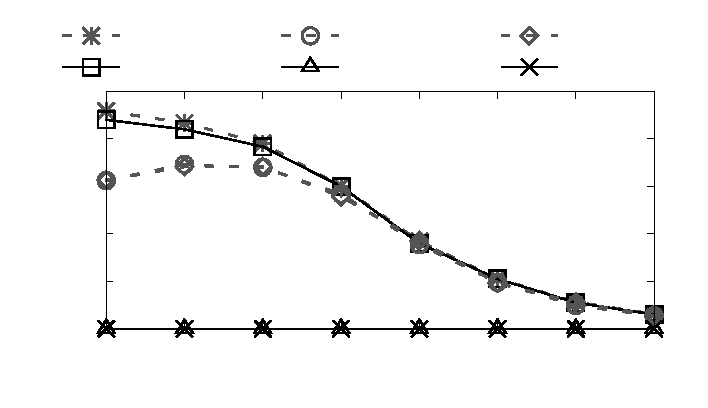
\includegraphics[width={324.00bp},height={180.00bp}]{spectre_normalS8W2}}%
    \gplfronttext
  \end{picture}%
\endgroup
}
\caption{\JaccardWithDeclass{\secretsSetSize} for \spectre in different procedures\label{fig:spectre:jaccard}}
\end{figure}

In generating interference rules for \proc with a long speculation
(\figref{code:assembly:spectre:long}), the linear feature
\begin{align*}
  \linearFeature{0} &
  = \begin{array}[t]{@{}l}
    0.005\times\SecFn{}(\secretVar)-0.003\times\SecFnAlt{}(\secretVar)
    -~0.494\times\ACIFn{}(\text{`offset'})+0.496\times\AIIFn{}(\text{`arr1.size'})
    \end{array}\\
  & \approx 0.5\times\AIIFn{}(\text{`arr1.size'}) - 0.5\times\ACIFn{}(\text{`offset'})
\end{align*}
and specifically the conjunct $\linearFeature{0} < 1$ appears in many
of the top ranked rules.  Using the approximation of \linearFeature{0}
above, $\linearFeature{0} < 1$ implies that
$\AIIFn{}(\text{`arr1.size'}) < \ACIFn{}(\text{`offset'}) + 2$, and so
the offset is indeed out-of-bounds.  An example top-ranked rule with
precision 1.0 and recall 0.30 is
\[
\begin{array}{r}
  \linearFeature{0}<1 \wedge \ACIFn{}(\bpdState{0})[1]<1 
  \wedge~\hfill\diffFeature{2}\ge 1 
\end{array}
\]
This rule indicates that an attacker can determine the third bit of
the secret when the second bit of the state of the prediction entry
$\ACIFn{}(\bpdState{0})$ is 0 (`strongly untaken') or 1 (`weakly
untaken').  Analogous rules appear in the list for each of bits 0-2
and 4 of the secret.  Other highly ranked rules (also with precision
1.0 and recall 0.30) are
\begin{align}
\begin{array}{r}
  \linearFeature{0}<1 \wedge \ACIFn{}(\bpdCFI{0})[0]\ge 1
  \wedge~\hfill\diffFeature{0}\ge 1
\end{array}
\label{eqn:spec-ruleTwo}\\
\begin{array}{r}
  \linearFeature{0}<1 \wedge \ACIFn{}(\bpdCFI{0})[1]<1 
  \wedge~\hfill\diffFeature{3}\ge 1 
\end{array}
\label{eqn:spec-ruleThree}
\end{align}
Rule \eqnref{eqn:spec-ruleTwo} leaks the first bit of the secret when
the `CFI' value (i.e., $\ACIFn{}(\bpdCFI{0})$) in the prediction entry
is 1 or 3, and \eqnref{eqn:spec-ruleThree} leaks the fourth bit when
the `CFI' value is 0 or 1.  In these cases, the `CFI' value does not
match the CFI portion of the instruction address (i.e., the address of
\lineref{line:spectre:branch} in \figref{code:assembly:spectre:long}),
which was \texttt{0x800000800} + \texttt{0x44}
(=~\texttt{0b0\colorbox{lightgrey}{10}\underline{00}100}), yielding a
CFI portion of \texttt{0b\colorbox{lightgrey}{10}} and \bpdIdx of
\texttt{0b\underline{00}}.  Because of the mismatch on CFI value,
$\ACIFn{}(\bpdState{0})$ is ignored and so speculation will not
execute
\linerefs{line:spectre:memaccess:start}{line:spectre:memaccess:end}.
Though \eqnref{eqn:spec-ruleTwo} and \eqnref{eqn:spec-ruleThree} are
specific to the first or fourth bit of the secret, respectively,
analogous rules appear for each of bits 0-3.

We have performed this evaluation using earlier \boom versions and
noticed that the out-of-bounds leakage was partially eliminated in version
2.2.3.\footnote{In \boom version 2.2.1, the victim program described
  in \figref{code:victim:spectre:short} also suffers the
  out-of-bounds leakage and thus has `shortDepend' close to
  `complexDepend' and `shortDepend+declass' close to
  `complexDepend+declass'.} Since that version, the miss handling
(MSHR) module of the L1 cache tracks branch prediction results and
discards the pending cache refill request if a misprediction is
detected before the refill commit. This change prevents the bounds
check bypass in \figref{code:victim:spectre:short}.

\subsection{Performance}
\label{dinome:sec:exp:performance}
In \thirdsysname, we have four important components: an automated logical
formula generator (\secref{dinome:sec:impl:logic}), a model counter
(\secref{dinome:sec:impl:counter}), a sampler (\secref{dinome:sec:impl:sampler}),
and a rule learner (\secref{dinome:sec:interpret:rules}).  This section
reports the time costs in the first three stages for all case studies
we have evaluated. We performed those experiments on a DELL PowerEdge
R815 server with 2.3\gigahertz AMD Opteron 6376 processors and
128\gigabytes memory.

The time to generate the logical postcondition is primarily influenced
by the number of RISC-V BOOM cycles represented by that postcondition,
as we incrementally compose the formula cycle by cycle.  Computing
\postcondition{\proc}{} required 20-40 minutes for the memory
accessing experiments (100 cycles) in \secref{dinome:sec:exp:cache} and
\secref{dinome:sec:exp:cachedefense}; 45 minutes for the modular
exponentiation experiments (120 cycles) in \secref{dinome:sec:exp:modexp};
and around 2 hours for the \spectre experiments (150 cycles) in
\secref{dinome:sec:exp:spectre}.

\figref{fig:cost:count} shows the runtime to compute \textit{one}
estimate of $\JaccardRand{}(\secretsSet{},\secretsSetAlt{})$ or
$\JaccardWithDeclass{}(\secretsSet{},\secretsSetAlt{})$ in the model
counting process; note the logarithmic y-axis.  Specifically, counting
for cache-based side channels in \scatterCache and \phantomCache are
much more expensive than others, where one estimate requires up to 16
minutes.  The difficulty in counting for \scatterCache (denoted by
`\scatterCacheAbbr') and \phantomCache (denoted by
`\phantomCacheAbbr') is due to the large size of their counting
variables.  For \scatterCache, the memory-to-cache mapping uses
$log_2(\cachesetNmbr) \times \cacheLineNmbr$ bits per domain per
memory block for 32 memory blocks. Specifically, the 8-way 2-set
\scatterCache (denoted by `\scatterCacheAbbr ($\cachesetNmbr=2$)'),
uses 512 bits to represent $\AIIFn{}(\cacheMap{})$, which means the
counting process would add hundreds of XOR constraints to compute one
estimate, which greatly increases the difficulty to find a feasible
solution.  To obtain the sample sets \interferenceSetSamples and
\noninterferenceSetSamples, the sampling process generates a tuple in
\interferenceSetSamples or \noninterferenceSetSamples within seconds,
as illustrated in \figref{fig:cost:sample}.

Our reported results reflect estimations of
$\JaccardRand{}(\secretsSet{},\secretsSetAlt{})$ or
$\JaccardWithDeclass{}(\secretsSet{},\secretsSetAlt{})$ for at least
100 \secretsSet{}, \secretsSetAlt{} pairs per \secretsSetSize, and we
sampled up to 100,000 tuples in \interferenceSetSamples and
\noninterferenceSetSamples.  These estimations and samplings are
trivially parallelizable and so, with horizontal scaling, can be
performed in total times approaching those in \figref{fig:cost:count}
and \figref{fig:cost:sample} to the extent budget allows.

\begin{figure}
\small{\resizebox{0.95\linewidth}{!}{\large% GNUPLOT: LaTeX picture with Postscript
\begingroup
  \makeatletter
  \providecommand\color[2][]{%
    \GenericError{(gnuplot) \space\space\space\@spaces}{%
      Package color not loaded in conjunction with
      terminal option `colourtext'%
    }{See the gnuplot documentation for explanation.%
    }{Either use 'blacktext' in gnuplot or load the package
      color.sty in LaTeX.}%
    \renewcommand\color[2][]{}%
  }%
  \providecommand\includegraphics[2][]{%
    \GenericError{(gnuplot) \space\space\space\@spaces}{%
      Package graphicx or graphics not loaded%
    }{See the gnuplot documentation for explanation.%
    }{The gnuplot epslatex terminal needs graphicx.sty or graphics.sty.}%
    \renewcommand\includegraphics[2][]{}%
  }%
  \providecommand\rotatebox[2]{#2}%
  \@ifundefined{ifGPcolor}{%
    \newif\ifGPcolor
    \GPcolortrue
  }{}%
  \@ifundefined{ifGPblacktext}{%
    \newif\ifGPblacktext
    \GPblacktexttrue
  }{}%
  % define a \g@addto@macro without @ in the name:
  \let\gplgaddtomacro\g@addto@macro
  % define empty templates for all commands taking text:
  \gdef\gplbacktext{}%
  \gdef\gplfronttext{}%
  \makeatother
  \ifGPblacktext
    % no textcolor at all
    \def\colorrgb#1{}%
    \def\colorgray#1{}%
  \else
    % gray or color?
    \ifGPcolor
      \def\colorrgb#1{\color[rgb]{#1}}%
      \def\colorgray#1{\color[gray]{#1}}%
      \expandafter\def\csname LTw\endcsname{\color{white}}%
      \expandafter\def\csname LTb\endcsname{\color{black}}%
      \expandafter\def\csname LTa\endcsname{\color{black}}%
      \expandafter\def\csname LT0\endcsname{\color[rgb]{1,0,0}}%
      \expandafter\def\csname LT1\endcsname{\color[rgb]{0,1,0}}%
      \expandafter\def\csname LT2\endcsname{\color[rgb]{0,0,1}}%
      \expandafter\def\csname LT3\endcsname{\color[rgb]{1,0,1}}%
      \expandafter\def\csname LT4\endcsname{\color[rgb]{0,1,1}}%
      \expandafter\def\csname LT5\endcsname{\color[rgb]{1,1,0}}%
      \expandafter\def\csname LT6\endcsname{\color[rgb]{0,0,0}}%
      \expandafter\def\csname LT7\endcsname{\color[rgb]{1,0.3,0}}%
      \expandafter\def\csname LT8\endcsname{\color[rgb]{0.5,0.5,0.5}}%
    \else
      % gray
      \def\colorrgb#1{\color{black}}%
      \def\colorgray#1{\color[gray]{#1}}%
      \expandafter\def\csname LTw\endcsname{\color{white}}%
      \expandafter\def\csname LTb\endcsname{\color{black}}%
      \expandafter\def\csname LTa\endcsname{\color{black}}%
      \expandafter\def\csname LT0\endcsname{\color{black}}%
      \expandafter\def\csname LT1\endcsname{\color{black}}%
      \expandafter\def\csname LT2\endcsname{\color{black}}%
      \expandafter\def\csname LT3\endcsname{\color{black}}%
      \expandafter\def\csname LT4\endcsname{\color{black}}%
      \expandafter\def\csname LT5\endcsname{\color{black}}%
      \expandafter\def\csname LT6\endcsname{\color{black}}%
      \expandafter\def\csname LT7\endcsname{\color{black}}%
      \expandafter\def\csname LT8\endcsname{\color{black}}%
    \fi
  \fi
    \setlength{\unitlength}{0.0500bp}%
    \ifx\gptboxheight\undefined%
      \newlength{\gptboxheight}%
      \newlength{\gptboxwidth}%
      \newsavebox{\gptboxtext}%
    \fi%
    \setlength{\fboxrule}{0.5pt}%
    \setlength{\fboxsep}{1pt}%
\begin{picture}(14400.00,3600.00)%
    \gplgaddtomacro\gplbacktext{%
      \csname LTb\endcsname%%
      \put(946,1459){\makebox(0,0)[r]{\strut{}$0.1$}}%
      \put(946,1818){\makebox(0,0)[r]{\strut{}$1$}}%
      \put(946,2177){\makebox(0,0)[r]{\strut{}$10$}}%
      \put(946,2536){\makebox(0,0)[r]{\strut{}$100$}}%
      \put(946,2895){\makebox(0,0)[r]{\strut{}$1000$}}%
      \put(1350,1327){\rotatebox{-28}{\makebox(0,0)[l]{\strut{}\normalCache($ \cachesetNmbr\!=\!1$)}}}%
      \put(1895,1327){\rotatebox{-28}{\makebox(0,0)[l]{\strut{}\normalCache($ \cachesetNmbr\!=\!2$)}}}%
      \put(2440,1327){\rotatebox{-28}{\makebox(0,0)[l]{\strut{}\normalCache($ \cachesetNmbr\!=\!4$)}}}%
      \put(2984,1327){\rotatebox{-28}{\makebox(0,0)[l]{\strut{}\normalCache($ \cachesetNmbr\!=\!8$)}}}%
      \put(3529,1327){\rotatebox{-28}{\makebox(0,0)[l]{\strut{}\normalCache($\cachesetNmbr\!=\!16$)}}}%
      \put(4074,1327){\rotatebox{-28}{\makebox(0,0)[l]{\strut{}\scatterCacheAbbr($ \cachesetNmbr\!=\!1$)}}}%
      \put(4618,1327){\rotatebox{-28}{\makebox(0,0)[l]{\strut{}\scatterCacheAbbr($ \cachesetNmbr\!=\!2$)}}}%
      \put(5163,1327){\rotatebox{-28}{\makebox(0,0)[l]{\strut{}\scatterCacheAbbr($ \cachesetNmbr\!=\!4$)}}}%
      \put(5707,1327){\rotatebox{-28}{\makebox(0,0)[l]{\strut{}\scatterCacheAbbr($ \cachesetNmbr\!=\!8$)}}}%
      \put(6252,1327){\rotatebox{-28}{\makebox(0,0)[l]{\strut{}\scatterCacheAbbr($\cachesetNmbr\!=\!16$)}}}%
      \put(6797,1327){\rotatebox{-28}{\makebox(0,0)[l]{\strut{}\phantomCacheAbbr($ \cachesetNmbr\!=\!1,\phantomR\!=\!1$)}}}%
      \put(7341,1327){\rotatebox{-28}{\makebox(0,0)[l]{\strut{}\phantomCacheAbbr($ \cachesetNmbr\!=\!4,\phantomR\!=\!1$)}}}%
      \put(7886,1327){\rotatebox{-28}{\makebox(0,0)[l]{\strut{}\phantomCacheAbbr($ \cachesetNmbr\!=\!8,\phantomR\!=\!1$)}}}%
      \put(8431,1327){\rotatebox{-28}{\makebox(0,0)[l]{\strut{}\phantomCacheAbbr($ \cachesetNmbr\!=\!16,\phantomR\!=\!2$)}}}%
      \put(8975,1327){\rotatebox{-28}{\makebox(0,0)[l]{\strut{}\phantomCacheAbbr($ \cachesetNmbr\!=\!4,\phantomR\!=\!2$)}}}%
      \put(9520,1327){\rotatebox{-28}{\makebox(0,0)[l]{\strut{}\phantomCacheAbbr($ \cachesetNmbr\!=\!8,\phantomR\!=\!2$)}}}%
      \put(10065,1327){\rotatebox{-28}{\makebox(0,0)[l]{\strut{}ShortSpec}}}%
      \put(10446,1327){\rotatebox{-28}{\makebox(0,0)[l]{\strut{}ShortSpec+\declassify{}}}}%
      \put(10827,1327){\rotatebox{-28}{\makebox(0,0)[l]{\strut{}LongSpec}}}%
      \put(11208,1327){\rotatebox{-28}{\makebox(0,0)[l]{\strut{}LongSpec+\declassify{}}}}%
      \put(11590,1327){\rotatebox{-28}{\makebox(0,0)[l]{\strut{}\modexp($\window\!=\!1$)}}}%
      \put(11971,1327){\rotatebox{-28}{\makebox(0,0)[l]{\strut{}\modexp($\window\!=\!2$)}}}%
      \put(12352,1327){\rotatebox{-28}{\makebox(0,0)[l]{\strut{}\modexp($\window\!=\!4$)}}}%
      \put(12733,1327){\rotatebox{-28}{\makebox(0,0)[l]{\strut{}\modexp($\window\!=\!6$)}}}%
      \put(13115,1327){\rotatebox{-28}{\makebox(0,0)[l]{\strut{}\modexp($\window\!=\!8$)}}}%
    }%
    \gplgaddtomacro\gplfronttext{%
      \csname LTb\endcsname%%
      \put(341,2177){\rotatebox{-270}{\makebox(0,0){\strut{}Time for one estimation (s)}}}%
      \csname LTb\endcsname%%
      \put(1669,3416){\makebox(0,0)[l]{\strut{}Unshared}}%
      \csname LTb\endcsname%%
      \put(1669,3174){\makebox(0,0)[l]{\strut{}Shared}}%
      \csname LTb\endcsname%%
      \put(5560,3416){\makebox(0,0)[l]{\strut{}Unshared ($\forall\blockIdx:\ACIFn{}(\loadVar)[\blockIdx]=1$)}}%
      \csname LTb\endcsname%%
      \put(5560,3174){\makebox(0,0)[l]{\strut{}Shared ($\forall \blockIdx: \ACIFn{}(\loadVar)[\blockIdx]=0$)}}%
    }%
    \gplbacktext
    \put(0,0){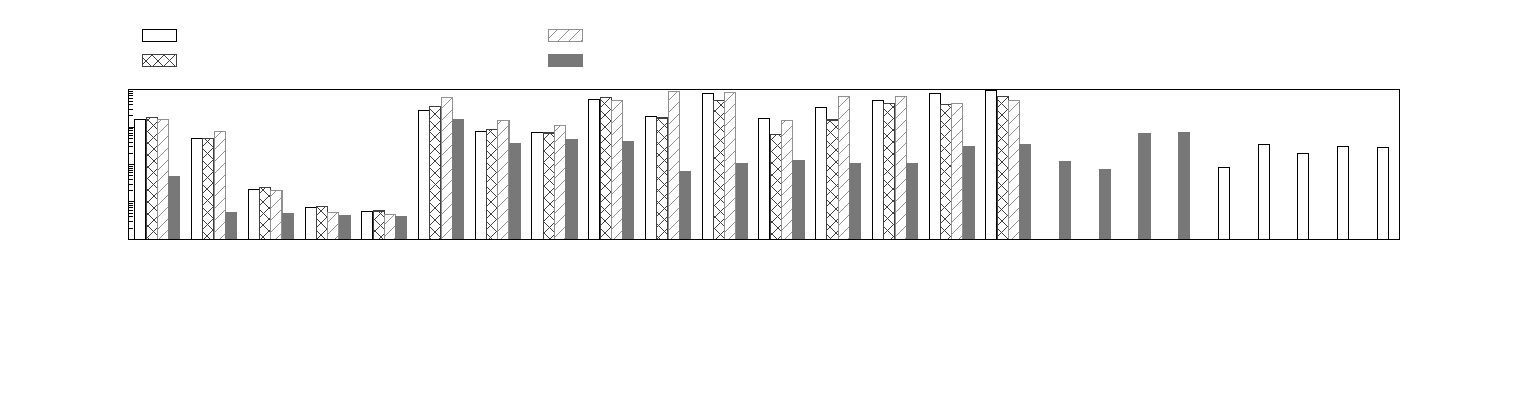
\includegraphics[width={720.00bp},height={180.00bp}]{time}}%
    \gplfronttext
  \end{picture}%
\endgroup
}}
\caption{Time used in one estimation of
  $\JaccardWithDeclass{}(\secretsSet{},\secretsSetAlt{})$
  \label{fig:cost:count}}
\end{figure}

\begin{figure}
\small{\resizebox{0.95\linewidth}{!}{\large% GNUPLOT: LaTeX picture with Postscript
\begingroup
  \makeatletter
  \providecommand\color[2][]{%
    \GenericError{(gnuplot) \space\space\space\@spaces}{%
      Package color not loaded in conjunction with
      terminal option `colourtext'%
    }{See the gnuplot documentation for explanation.%
    }{Either use 'blacktext' in gnuplot or load the package
      color.sty in LaTeX.}%
    \renewcommand\color[2][]{}%
  }%
  \providecommand\includegraphics[2][]{%
    \GenericError{(gnuplot) \space\space\space\@spaces}{%
      Package graphicx or graphics not loaded%
    }{See the gnuplot documentation for explanation.%
    }{The gnuplot epslatex terminal needs graphicx.sty or graphics.sty.}%
    \renewcommand\includegraphics[2][]{}%
  }%
  \providecommand\rotatebox[2]{#2}%
  \@ifundefined{ifGPcolor}{%
    \newif\ifGPcolor
    \GPcolortrue
  }{}%
  \@ifundefined{ifGPblacktext}{%
    \newif\ifGPblacktext
    \GPblacktexttrue
  }{}%
  % define a \g@addto@macro without @ in the name:
  \let\gplgaddtomacro\g@addto@macro
  % define empty templates for all commands taking text:
  \gdef\gplbacktext{}%
  \gdef\gplfronttext{}%
  \makeatother
  \ifGPblacktext
    % no textcolor at all
    \def\colorrgb#1{}%
    \def\colorgray#1{}%
  \else
    % gray or color?
    \ifGPcolor
      \def\colorrgb#1{\color[rgb]{#1}}%
      \def\colorgray#1{\color[gray]{#1}}%
      \expandafter\def\csname LTw\endcsname{\color{white}}%
      \expandafter\def\csname LTb\endcsname{\color{black}}%
      \expandafter\def\csname LTa\endcsname{\color{black}}%
      \expandafter\def\csname LT0\endcsname{\color[rgb]{1,0,0}}%
      \expandafter\def\csname LT1\endcsname{\color[rgb]{0,1,0}}%
      \expandafter\def\csname LT2\endcsname{\color[rgb]{0,0,1}}%
      \expandafter\def\csname LT3\endcsname{\color[rgb]{1,0,1}}%
      \expandafter\def\csname LT4\endcsname{\color[rgb]{0,1,1}}%
      \expandafter\def\csname LT5\endcsname{\color[rgb]{1,1,0}}%
      \expandafter\def\csname LT6\endcsname{\color[rgb]{0,0,0}}%
      \expandafter\def\csname LT7\endcsname{\color[rgb]{1,0.3,0}}%
      \expandafter\def\csname LT8\endcsname{\color[rgb]{0.5,0.5,0.5}}%
    \else
      % gray
      \def\colorrgb#1{\color{black}}%
      \def\colorgray#1{\color[gray]{#1}}%
      \expandafter\def\csname LTw\endcsname{\color{white}}%
      \expandafter\def\csname LTb\endcsname{\color{black}}%
      \expandafter\def\csname LTa\endcsname{\color{black}}%
      \expandafter\def\csname LT0\endcsname{\color{black}}%
      \expandafter\def\csname LT1\endcsname{\color{black}}%
      \expandafter\def\csname LT2\endcsname{\color{black}}%
      \expandafter\def\csname LT3\endcsname{\color{black}}%
      \expandafter\def\csname LT4\endcsname{\color{black}}%
      \expandafter\def\csname LT5\endcsname{\color{black}}%
      \expandafter\def\csname LT6\endcsname{\color{black}}%
      \expandafter\def\csname LT7\endcsname{\color{black}}%
      \expandafter\def\csname LT8\endcsname{\color{black}}%
    \fi
  \fi
    \setlength{\unitlength}{0.0500bp}%
    \ifx\gptboxheight\undefined%
      \newlength{\gptboxheight}%
      \newlength{\gptboxwidth}%
      \newsavebox{\gptboxtext}%
    \fi%
    \setlength{\fboxrule}{0.5pt}%
    \setlength{\fboxsep}{1pt}%
\begin{picture}(14400.00,3600.00)%
    \gplgaddtomacro\gplbacktext{%
      \csname LTb\endcsname%%
      \put(1210,1459){\makebox(0,0)[r]{\strut{}$0.0001$}}%
      \put(1210,1746){\makebox(0,0)[r]{\strut{}$0.001$}}%
      \put(1210,2033){\makebox(0,0)[r]{\strut{}$0.01$}}%
      \put(1210,2321){\makebox(0,0)[r]{\strut{}$0.1$}}%
      \put(1210,2608){\makebox(0,0)[r]{\strut{}$1$}}%
      \put(1210,2895){\makebox(0,0)[r]{\strut{}$10$}}%
      \put(1608,1327){\rotatebox{-28}{\makebox(0,0)[l]{\strut{}\normalCache($ \cachesetNmbr\!=\!1$)}}}%
      \put(2141,1327){\rotatebox{-28}{\makebox(0,0)[l]{\strut{}\normalCache($ \cachesetNmbr\!=\!2$)}}}%
      \put(2674,1327){\rotatebox{-28}{\makebox(0,0)[l]{\strut{}\normalCache($ \cachesetNmbr\!=\!4$)}}}%
      \put(3207,1327){\rotatebox{-28}{\makebox(0,0)[l]{\strut{}\normalCache($ \cachesetNmbr\!=\!8$)}}}%
      \put(3740,1327){\rotatebox{-28}{\makebox(0,0)[l]{\strut{}\normalCache($\cachesetNmbr\!=\!16$)}}}%
      \put(4273,1327){\rotatebox{-28}{\makebox(0,0)[l]{\strut{}\scatterCacheAbbr($ \cachesetNmbr\!=\!1$)}}}%
      \put(4806,1327){\rotatebox{-28}{\makebox(0,0)[l]{\strut{}\scatterCacheAbbr($ \cachesetNmbr\!=\!2$)}}}%
      \put(5339,1327){\rotatebox{-28}{\makebox(0,0)[l]{\strut{}\scatterCacheAbbr($ \cachesetNmbr\!=\!4$)}}}%
      \put(5872,1327){\rotatebox{-28}{\makebox(0,0)[l]{\strut{}\scatterCacheAbbr($ \cachesetNmbr\!=\!8$)}}}%
      \put(6405,1327){\rotatebox{-28}{\makebox(0,0)[l]{\strut{}\scatterCacheAbbr($\cachesetNmbr\!=\!16$)}}}%
      \put(6938,1327){\rotatebox{-28}{\makebox(0,0)[l]{\strut{}\phantomCacheAbbr($ \cachesetNmbr\!=\!1,\phantomR\!=\!1$)}}}%
      \put(7471,1327){\rotatebox{-28}{\makebox(0,0)[l]{\strut{}\phantomCacheAbbr($ \cachesetNmbr\!=\!4,\phantomR\!=\!1$)}}}%
      \put(8004,1327){\rotatebox{-28}{\makebox(0,0)[l]{\strut{}\phantomCacheAbbr($ \cachesetNmbr\!=\!8,\phantomR\!=\!1$)}}}%
      \put(8537,1327){\rotatebox{-28}{\makebox(0,0)[l]{\strut{}\phantomCacheAbbr($ \cachesetNmbr\!=\!16,\phantomR\!=\!2$)}}}%
      \put(9070,1327){\rotatebox{-28}{\makebox(0,0)[l]{\strut{}\phantomCacheAbbr($ \cachesetNmbr\!=\!4,\phantomR\!=\!2$)}}}%
      \put(9603,1327){\rotatebox{-28}{\makebox(0,0)[l]{\strut{}\phantomCacheAbbr($ \cachesetNmbr\!=\!8,\phantomR\!=\!2$)}}}%
      \put(10136,1327){\rotatebox{-28}{\makebox(0,0)[l]{\strut{}ShortSpec}}}%
      \put(10510,1327){\rotatebox{-28}{\makebox(0,0)[l]{\strut{}ShortSpec+\declassify{}}}}%
      \put(10883,1327){\rotatebox{-28}{\makebox(0,0)[l]{\strut{}LongSpec}}}%
      \put(11256,1327){\rotatebox{-28}{\makebox(0,0)[l]{\strut{}LongSpec+\declassify{}}}}%
      \put(11629,1327){\rotatebox{-28}{\makebox(0,0)[l]{\strut{}\modexp($\window\!=\!1$)}}}%
      \put(12002,1327){\rotatebox{-28}{\makebox(0,0)[l]{\strut{}\modexp($\window\!=\!2$)}}}%
      \put(12375,1327){\rotatebox{-28}{\makebox(0,0)[l]{\strut{}\modexp($\window\!=\!4$)}}}%
      \put(12748,1327){\rotatebox{-28}{\makebox(0,0)[l]{\strut{}\modexp($\window\!=\!6$)}}}%
      \put(13121,1327){\rotatebox{-28}{\makebox(0,0)[l]{\strut{}\modexp($\window\!=\!8$)}}}%
    }%
    \gplgaddtomacro\gplfronttext{%
      \csname LTb\endcsname%%
      \put(341,2177){\rotatebox{-270}{\makebox(0,0){\strut{}Time for one estimation (s)}}}%
      \csname LTb\endcsname%%
      \put(1933,3416){\makebox(0,0)[l]{\strut{}Unshared-\interferenceSetSamples}}%
      \csname LTb\endcsname%%
      \put(1933,3174){\makebox(0,0)[l]{\strut{}Shared-\interferenceSetSamples}}%
      \csname LTb\endcsname%%
      \put(5824,3416){\makebox(0,0)[l]{\strut{}Shared($\forall \blockIdx: \ACIFn{}(\loadVar)[\blockIdx]=0$)-\interferenceSetSamples}}%
      \csname LTb\endcsname%%
      \put(5824,3174){\makebox(0,0)[l]{\strut{}Unshared-\noninterferenceSetSamples}}%
      \csname LTb\endcsname%%
      \put(9715,3416){\makebox(0,0)[l]{\strut{}Shared-\noninterferenceSetSamples}}%
      \csname LTb\endcsname%%
      \put(9715,3174){\makebox(0,0)[l]{\strut{}Shared($\forall \blockIdx: \ACIFn{}(\loadVar)[\blockIdx]=0$)-\noninterferenceSetSamples}}%
    }%
    \gplbacktext
    \put(0,0){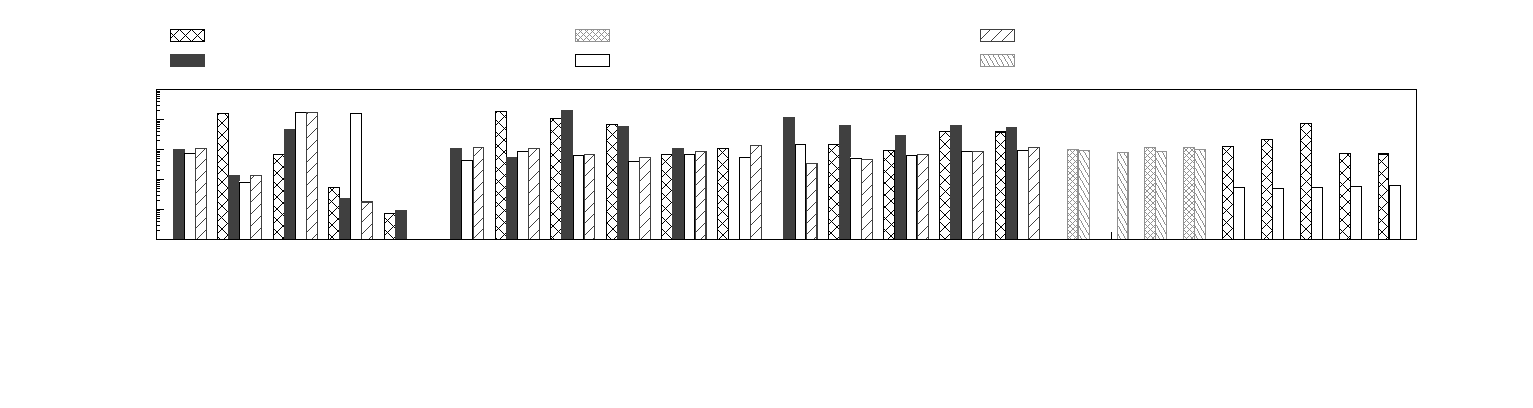
\includegraphics[width={720.00bp},height={180.00bp}]{sampletime}}%
    \gplfronttext
  \end{picture}%
\endgroup
}}
\caption{Time used in generating one tuple in
\noninterferenceSetSamples or
\interferenceSetSamples \label{fig:cost:sample}}
\end{figure}

\section{Limitations}
\label{dinome:sec:limitations}

\iffalse
\zz{runtime is limited by the solving time in SAT solver}
\zz{Current design cannot be scaled to unlimited number of CPU cycles.}
\zz{We cannot guarantee the compeleteness of the interference rules. Interpretable rules may skip the rule that only cover a small
portion of samples (i.e., with low recall). A possible solution is to
use the learned interference rule in declassification and run the
learning process again to get more coverage.}
\fi

Despite the scalability improvements represented by \thirdsysname
specifically for analyzing processor designs, it still has
limitations.  First, due to the complexity of hardware logic,
generating the postcondition $\postcondition{\proc}{}(\ACIFn{},
\AIIFn{}, \SecFn{}, \AOOFn{})$ for a \proc representing both the OS
and the application would require more CPU cycles than the number to
which we have been able to scale \thirdsysname thus far.  The \thirdsysname
workloads described in this chapter represent a tradeoff, using a
sequence of opcodes with concretized operations and selected symbolic
operands above a partially symbolic hardware specification.  To
evaluate with more complicated software, a possible solution is to
highly concretize the initial hardware state (especially for the
memory and cache states) or highly concretize the software, at the
cost of possibly missing some potential leakage that remains hidden
due to this concretization.

A second limitation of \thirdsysname, and specifically of its generation of
interpretation rules to explain leakage, is that the interpretation
rules may not be complete, for two reasons.  First, the interpretation
rules might skip a rule that only covers a small portion of leakage
samples (i.e., with low recall).  A possible solution to address this
source of incompleteness is to declassify the sources of leakage
exposed in the inference rules that \textit{are} learned, and then
rerun the learning process again. Second, the conditions that result in
leakage might be more complicated than can be learned using decision
trees built using local linear classifiers.  To address this
incompleteness, alternative learning methods might be tried, though
doing so while retaining interpretability will be a challenge.

\section{Summary}
\label{dinome:sec:summary}

Scaling high-fidelity, static noninterference measurement to complex
computations has been a challenge since the introduction of
noninterference in the 1980's~\cite{goguen1982security}.  We believe
that we have advanced the state-of-the-art in this area both generally
and specifically for its application to processor designs.  Certain
innovations in our \thirdsysname framework, such as the cycle-by-cycle
construction of the logical postcondition for processor execution, are
specific to processor designs.  Others, such as our methods for
declassification and interpreting leakage results, are not.  Together,
however, they permit the measurement of leakage in complex scenarios,
as we demonstrated through using \thirdsysname to analyze leakage due to
speculative execution in the \boom core and of published defenses to
mitigate it.  Our analysis enables comparisons between defenses to
discover, e.g., the processor and defense parameterizations where one
defense outperforms the other.  Though the performance of \thirdsysname
suggests that static measurement of noninterference for processors is
still too time-intensive for highly interactive use, it is fast enough
to permit multiple analysis iterations per day in many cases.  And
through its improvements in declassification and interpretability, it
substantially facilitates human understanding of its measurement
results.

\iffalse
Evaluating unintended information leakage is essential for both software
and hardware designs.  We proposed a novel methodology to
evaluate the information leaks based on a declassification-sensitive
noninterference property, which rules out the interference caused by
the expected declassification policy.  Intuitively, we think a system
is not secure if we can distinguish between secrets that could not be
inferred by the allowed declassification information through
observables. As an implementation prototype, our \thirdsysname is designed
to analyze the hardware and software combined vulnerabilities, standing
on the shoulders of state-of-art formal methods. Our \thirdsysname
transforms a high-complexity task to many hash-based scalable works,
using various optimizations in \sat and model counting areas.

Besides, we proposed a novel approach to find and explain the cause of
interference using interpretable machine learning. Instead of purely
relying on human effort to hypothesize and summarize the vulnerability
in complicated code snippets or limited examples, our interpretation
rules could reveal the condition when a pair of secrets
could be distinguished. Our case studies demonstrate that 
\begin{compactitem}
\item
The quantified measure \JaccardWithDeclass{\secretsSetSize} is useful
to compare unintended leakage in different hardware and software implementations.
\item The explanation could even reveal both low-level hardware logic
and high-level software logic that breaks the noninterference property
in a combined format. This could be useful when the coding style is not
that friendly to humans (e.g., \boom's Verilog code automatically
generated from Chisel). 
\end{compactitem}
\if
0
To locate all sources of interference, We can apply the
gradient boosting idea to the sampling generation which first learn the
interference rules uses samplings of \noninterferenceSetSamples and
\interferenceSetSamples, then focus on solutions following the learned
noninterference rules from the sets by asserting the conjunction of the
noninterference predicates is true to find a more fine-grained
interference rule not included in your previous learning. To 
\fi
\fi

